\documentclass[twoside]{book}

% Packages required by doxygen
\usepackage{fixltx2e}
\usepackage{calc}
\usepackage{doxygen}
\usepackage{graphicx}
\usepackage[utf8]{inputenc}
\usepackage{makeidx}
\usepackage{multicol}
\usepackage{multirow}
\PassOptionsToPackage{warn}{textcomp}
\usepackage{textcomp}
\usepackage[nointegrals]{wasysym}
\usepackage[table]{xcolor}

% Font selection
\usepackage[T1]{fontenc}
\usepackage{mathptmx}
\usepackage[scaled=.90]{helvet}
\usepackage{courier}
\usepackage{amssymb}
\usepackage{sectsty}
\renewcommand{\familydefault}{\sfdefault}
\allsectionsfont{%
  \fontseries{bc}\selectfont%
  \color{darkgray}%
}
\renewcommand{\DoxyLabelFont}{%
  \fontseries{bc}\selectfont%
  \color{darkgray}%
}
\newcommand{\+}{\discretionary{\mbox{\scriptsize$\hookleftarrow$}}{}{}}

% Page & text layout
\usepackage{geometry}
\geometry{%
  a4paper,%
  top=2.5cm,%
  bottom=2.5cm,%
  left=2.5cm,%
  right=2.5cm%
}
\tolerance=750
\hfuzz=15pt
\hbadness=750
\setlength{\emergencystretch}{15pt}
\setlength{\parindent}{0cm}
\setlength{\parskip}{0.2cm}
\makeatletter
\renewcommand{\paragraph}{%
  \@startsection{paragraph}{4}{0ex}{-1.0ex}{1.0ex}{%
    \normalfont\normalsize\bfseries\SS@parafont%
  }%
}
\renewcommand{\subparagraph}{%
  \@startsection{subparagraph}{5}{0ex}{-1.0ex}{1.0ex}{%
    \normalfont\normalsize\bfseries\SS@subparafont%
  }%
}
\makeatother

% Headers & footers
\usepackage{fancyhdr}
\pagestyle{fancyplain}
\fancyhead[LE]{\fancyplain{}{\bfseries\thepage}}
\fancyhead[CE]{\fancyplain{}{}}
\fancyhead[RE]{\fancyplain{}{\bfseries\leftmark}}
\fancyhead[LO]{\fancyplain{}{\bfseries\rightmark}}
\fancyhead[CO]{\fancyplain{}{}}
\fancyhead[RO]{\fancyplain{}{\bfseries\thepage}}
\fancyfoot[LE]{\fancyplain{}{}}
\fancyfoot[CE]{\fancyplain{}{}}
\fancyfoot[RE]{\fancyplain{}{\bfseries\scriptsize Generated on Thu Jun 26 2014 15\+:29\+:50 for fcparsers by Doxygen }}
\fancyfoot[LO]{\fancyplain{}{\bfseries\scriptsize Generated on Thu Jun 26 2014 15\+:29\+:50 for fcparsers by Doxygen }}
\fancyfoot[CO]{\fancyplain{}{}}
\fancyfoot[RO]{\fancyplain{}{}}
\renewcommand{\footrulewidth}{0.4pt}
\renewcommand{\chaptermark}[1]{%
  \markboth{#1}{}%
}
\renewcommand{\sectionmark}[1]{%
  \markright{\thesection\ #1}%
}

% Indices & bibliography
\usepackage{natbib}
\usepackage[titles]{tocloft}
\setcounter{tocdepth}{3}
\setcounter{secnumdepth}{5}
\makeindex

% Custom commands
\newcommand{\clearemptydoublepage}{%
  \newpage{\pagestyle{empty}\cleardoublepage}%
}


%===== C O N T E N T S =====

\begin{document}

% Titlepage & ToC
\pagenumbering{roman}
\begin{titlepage}
\vspace*{7cm}
\begin{center}%
{\Large fcparsers \\[1ex]\large 0.\+3-\/123 }\\
\vspace*{1cm}
{\large Generated by Doxygen 1.8.7}\\
\vspace*{0.5cm}
{\small Thu Jun 26 2014 15:29:50}\\
\end{center}
\end{titlepage}
\clearemptydoublepage
\tableofcontents
\clearemptydoublepage
\pagenumbering{arabic}

%--- Begin generated contents ---
\chapter{Compatible File Formats}
\label{formats}
\doxyref{Brocade \char`\"{}alishow\char`\"{} and \char`\"{}zoneshow\char`\"{}}{p.}{AliShowZoneParser}

\doxyref{B\+N\+A Database}{p.}{BNAPURLConnection}

\doxyref{B\+N\+A Database}{p.}{BNAZoneParser}

\doxyref{Cisco \char`\"{}show device-\/alias database\char`\"{}}{p.}{DeviceAliasParser}

\doxyref{O\+C\+I Database}{p.}{DWHURLConnection}

\doxyref{O\+C\+I Database}{p.}{MSDWHURLConnection}

\doxyref{O\+C\+I Database}{p.}{OSMURLConnection}

\doxyref{Cisco \char`\"{}show zone\char`\"{}}{p.}{ShowZoneParser}

\doxyref{Virtual\+Wisdom4 Validation Errors}{p.}{VW4InvalidAdded} \section{Brocade \char`\"{}alishow\char`\"{} and \char`\"{}zoneshow\char`\"{}}\label{AliShowZoneParser}
The \doxyref{Ali\+Show\+Zone\+Parser}{p.}{classorg_1_1smallfoot_1_1parser_1_1zone_1_1AliShowZoneParser} parses the output of a Brocade S\+A\+N switch with the \char`\"{}alishow\char`\"{} or \char`\"{}zoneshow\char`\"{} commands.

As always, this parser is more successful when the content is treated like binary\+: don't edit it. In particular, the use of a putty log to capture output while querying the switch leads to parser exceptions because the interactive "you have connected to blah blah system version 1.\+2.\+3, the weather is fabulous and I have 42 pages of boilerplate to spit out before you enter the command for aliases... hit enter to continue... have some backspaces..." is included. As are the backspaces.

When collecting aliases using an ssh command, it's better to execute that command noninteractively\+:

In U\+N\+I\+X, Linux, Ubuntu, O\+S\+X, or the 6000 other licensees of the U\+S\+L codebase\+: \begin{DoxyVerb}ssh username@switch44.example.com "alishow" > switch44.alishow
\end{DoxyVerb}


In windows, using the {\tt putty} tools\+: \begin{DoxyVerb}plink.exe -l username -pw p4ssw0rd switch44.example.com "alishow" > switch44.alishow
\end{DoxyVerb}


This leads to a better chance to parse 100\% of the output with more accuracy, but I guess following this recommendation is up to the user, and to the engineer suggesting how he or she should collect the text for parsing.

\begin{DoxyVerb}Defined configuration:
 cfg:   SAN_CFG_B
                SANASVR001_FabA; SANASVR002_FabA; SANASVR003_FabA;
                SANASVR004_FabA
 alias: HDS0123457_CL3E
                50:06:0e:80:12:34:57:24
 alias: HDS0123457_CL3F
                50:06:0e:80:12:34:57:25
 alias: HDS0123457_CL5E
                50:06:0e:80:12:34:57:44
 alias: HDS0123457_CL5F
                50:06:0e:80:12:34:57:45
 alias: HDS0123457_CL7E
                50:06:0e:80:12:34:57:64
 alias: HDS0123457_CL7F
                50:06:0e:80:12:34:57:65
 alias: Oracle_123466
                10:00:00:00:c9:12:34:66
 alias: Oracle_123467
                10:00:00:00:c9:12:34:67
 alias: NASHead_123468
                10:00:00:00:c9:12:34:68
 alias: NASHead_123469
                10:00:00:00:c9:12:34:69
 alias: NASMany_654321
                10:00:00:00:c9:44:44:10; 10:00:00:00:c9:44:44:11
                10:00:00:00:c9:44:44:20; 10:00:00:00:c9:44:44:21
                10:00:00:00:c9:44:44:30; 10:00:00:00:c9:44:44:31

Effective configuration:
 cfg:   SAN_CFG_B
 zone:  SANASVR001_FabA
                10:00:00:00:c9:12:34:66 \end{DoxyVerb}


The result is a list of nicknames, such as\+:

\begin{DoxyVerb}50060e8012345724,HDS0123457_CL3E
50060e8012345725,"HDS0123457_CL3F"
50060e8012345744,"HDS0123457_CL5E"
50060e8012345745,"HDS0123457_CL5F"
50060e8012345764,"HDS0123457_CL7E"
50060e8012345765,"HDS0123457_CL7F"
10000000c9123466,"Oracle_123466"
10000000c9123467,"Oracle_123467"
10000000c9123468,"NASHead_123468"
10000000c9123469,"NASHead_123469"
10000000c9444410,"NASMany_654321"
10000000c9444411,"NASMany_654321"
10000000c9444420,"NASMany_654321"
10000000c9444421,"NASMany_654321"
10000000c9444430,"NASMany_654321"
10000000c9444431,"NASMany_654321" \end{DoxyVerb}
 \section{B\+N\+A Database}\label{BNAPURLConnection}
The \doxyref{B\+N\+A\+P\+U\+R\+L\+Connection}{p.}{classorg_1_1smallfoot_1_1parser_1_1bnapsql_1_1BNAPURLConnection} collects bna\+://, bnapsql\+://, cmcne\+://, and dcfm\+:// sources from B\+N\+A's backend database to provide the bnazone-\/formatted zone and alias information

This collector/parser chain is more successful than text-\/based parsers simply because it avoids human-\/error and the error of not reading the warning to avoid putty log traces and other \char`\"{}nearly 100\% unmodified\char`\"{} methods of transferring content. Additionally, this is an entirely binary connection, so the user cannot accidentally edit the content. Finally, as B\+N\+A may harvest from and provide config to many fabrics at once, this is typically \char`\"{}a broader net to cast\char`\"{} to collect information. \section{B\+N\+A Database}\label{BNAZoneParser}
The \doxyref{B\+N\+A\+Zone\+Parser}{p.}{classorg_1_1smallfoot_1_1parser_1_1zone_1_1BNAZoneParser} parses the binary text records in a B\+N\+A server representing the zonesets and their aliases

This parser is not normally used from a downloaded text; it's normally used when a client executes a query against the backing database of a B\+N\+A instance. The resulting query tends to have data columns in resultset that are binary-\/coded to reduce parsing load. These same binary tokens are parsed by \doxyref{B\+N\+A\+Zone\+Parser}{p.}{classorg_1_1smallfoot_1_1parser_1_1zone_1_1BNAZoneParser} to provide results similar to Ali\+Show\+Parser.

There are times that the backing database is easier to query than switches

Use this parser automatically by collecting using a bnapsql\+:// U\+R\+L protocol with the \char`\"{}vict\char`\"{} or \char`\"{}vw4tools\char`\"{} project. For example\+: \begin{DoxyVerb}java -jar vict.jar -N bnapsql://bna.example.com/
\end{DoxyVerb}


or \begin{DoxyVerb}java -jar vw4tools.jar -N bna://bna.example.com/\end{DoxyVerb}
 \section{Cisco \char`\"{}show device-\/alias database\char`\"{}}\label{DeviceAliasParser}
The \doxyref{Device\+Alias\+Parser}{p.}{classorg_1_1smallfoot_1_1parser_1_1zone_1_1DeviceAliasParser} parses the output of a Cisco S\+A\+N switch with the \char`\"{}show device-\/alias database\char`\"{} command

As always, this parser is more successful when the content is treated like binary\+: don't edit it. In particular, the use of a putty log to capture output while querying the switch leads to parser exceptions because the interactive "you have connected to blah blah system version 1.\+2.\+3, the weather is fabulous and I have 42 pages of boilerplate to spit out before you enter the command for aliases... hit enter to continue... have some backspaces..." is included. As are the backspaces.

When collecting aliases using an ssh command, it's better to execute that command noninteractively\+:

In U\+N\+I\+X, Linux, Ubuntu, O\+S\+X, or the 6000 other licensees of the U\+S\+L codebase\+: \begin{DoxyVerb}ssh username@switch44.example.com "show device-alias database" > switch44.dad
\end{DoxyVerb}


In windows, using the {\tt putty} tools\+: \begin{DoxyVerb}plink.exe -l username -pw p4ssw0rd switch44.example.com "show device-alias database" > switch44.dad
\end{DoxyVerb}


This leads to a better chance to parse 100\% of the output with more accuracy, but I guess following this recommendation is up to the user, and to the engineer suggesting how he or she should collect the text for parsing.

\begin{DoxyVerb}The copyrights to certain works contained in this software are
owned by other third parties and used and distributed under
license. Certain components of this software are licensed under
the GNU General Public License (GPL) version 2.0 or the GNU
Lesser General Public License (LGPL) Version 2.1. A copy of each
such license is available at
http://www.opensource.org/licenses/gpl-2.0.php and
http://www.opensource.org/licenses/lgpl-2.1.php
switch44a# show device-alias database
device-alias name server44_hba0 pwwn 10:00:00:00:c9:12:34:56
device-alias name server44_hba1 pwwn 10:00:00:00:c9:12:34:57
device-alias name oracle10_hba0 pwwn 21:00:00:24:ff:12:34:56
device-alias name oracle10_hba1 pwwn 22:00:00:24:ff:12:34:56
device-alias name vmax-18641-fa06a0 pwwn 50:00:09:72:01:23:45:54
device-alias name vmax-18641-fa07a0 pwwn 50:00:09:72:01:23:45:58 \end{DoxyVerb}


with the following result of W\+W\+P\+N/alias pairs\+: \begin{DoxyVerb}10000000c9123456,"server44_hba0"
10000000c9123457,"server44_hba1"
21000024ff123456,"oracle10_hba0"
22000024ff123456,"oracle10_hba1"
5000097201234554,"vmax-18641-fa06a0"
5000097201234558,"vmax-18641-fa07a0" \end{DoxyVerb}
 \section{O\+C\+I Database}\label{DWHURLConnection}
The \doxyref{D\+W\+H\+U\+R\+L\+Connection}{p.}{classorg_1_1smallfoot_1_1parser_1_1ocidwh_1_1DWHURLConnection} collects ocidwh\+:// sources from O\+C\+I's backend database to search for aliases

This collector/parser chain is more successful than text-\/based parsers simply because it avoids human-\/error and the error of not reading the warning to avoid putty log traces and other \char`\"{}nearly 100\% unmodified\char`\"{} methods of transferring content. Additionally, this is an entirely binary connection, so the user cannot accidentally edit the content. Finally, as B\+N\+A may harvest from and provide config to many fabrics at once, this is typically \char`\"{}a broader net to cast\char`\"{} to collect information. \section{O\+C\+I Database}\label{MSDWHURLConnection}
The \doxyref{M\+S\+D\+W\+H\+U\+R\+L\+Connection}{p.}{classorg_1_1smallfoot_1_1parser_1_1msosmsql_1_1MSDWHURLConnection} collects msosmsql\+:// sources from O\+C\+I's backend database to search for aliases

This collector/parser chain is more successful than text-\/based parsers simply because it avoids human-\/error and the error of not reading the warning to avoid putty log traces and other \char`\"{}nearly 100\% unmodified\char`\"{} methods of transferring content. Additionally, this is an entirely binary connection, so the user cannot accidentally edit the content. Finally, as B\+N\+A may harvest from and provide config to many fabrics at once, this is typically \char`\"{}a broader net to cast\char`\"{} to collect information. \section{O\+C\+I Database}\label{OSMURLConnection}
The \doxyref{O\+S\+M\+U\+R\+L\+Connection}{p.}{classorg_1_1smallfoot_1_1parser_1_1osmsql_1_1OSMURLConnection} collects osmsql\+:// sources from O\+C\+I's backend database to parse for aliases it may know

This collector/parser chain is more successful than text-\/based parsers simply because it avoids human-\/error and the error of not reading the warning to avoid putty log traces and other \char`\"{}nearly 100\% unmodified\char`\"{} methods of transferring content. Additionally, this is an entirely binary connection, so the user cannot accidentally edit the content. Finally, as B\+N\+A may harvest from and provide config to many fabrics at once, this is typically \char`\"{}a broader net to cast\char`\"{} to collect information.

Testing of this data was done with an exported config database from jessigg called \char`\"{}dwh\+\_\+inventory.\+sql\char`\"{} loaded using\+: /usr/local/mysql/bin/mysqladmin create dwh\+\_\+inventory /usr/local/mysql/bin/mysql -\/u root mysql \char`\"{}grant connect on dwh\+\_\+inventory.$\ast$ to dwh identified by 'password'\char`\"{} /usr/local/mysql/bin/mysqladmin reload grant /usr/local/mysql/bin/mysql -\/u root dwh\+\_\+inventory $<$ $\sim$/dwh\+\_\+inventory.sql \section{Cisco \char`\"{}show zone\char`\"{}}\label{ShowZoneParser}
The \doxyref{Show\+Zone\+Parser}{p.}{classorg_1_1smallfoot_1_1parser_1_1zone_1_1ShowZoneParser} parses the output of a Cisco S\+A\+N switch with the \char`\"{}show zone\char`\"{} command

As always, this parser is more successful when the content is treated like binary\+: don't edit it. In particular, the use of a putty log to capture output while querying the switch leads to parser exceptions because the interactive "you have connected to blah blah system version 1.\+2.\+3, the weather is fabulous and I have 42 pages of boilerplate to spit out before you enter the command for aliases... hit enter to continue... have some backspaces..." is included. As are the backspaces.

When collecting aliases using an ssh command, it's better to execute that command noninteractively\+:

In U\+N\+I\+X, Linux, Ubuntu, O\+S\+X, or the 6000 other licensees of the U\+S\+L codebase\+: \begin{DoxyVerb}ssh username@switch44.example.com "show zone" > switch44.shzone
\end{DoxyVerb}


In windows, using the {\tt putty} tools\+: \begin{DoxyVerb}plink.exe -l username -pw p4ssw0rd switch44.example.com "show zone" > switch44.shzone
\end{DoxyVerb}


This leads to a better chance to parse 100\% of the output with more accuracy, but I guess following this recommendation is up to the user, and to the engineer suggesting how he or she should collect the text for parsing.

\begin{DoxyVerb}zone name SANASVR001_FabA vsan 100
  fcalias name Oracle_123466 vsan 100
    pwwn 10:00:00:00:c9:12:34:66

  fcalias name HDS0123457_CL7F vsan 100
    pwwn 50:06:0e:80:12:34:56:78

  fcalias name HDS0123457_CL7F vsan 100
    pwwn 50:06:0e:80:12:34:56:79

zone name SANASVR002_FabA vsan 100
  fcalias name Oracle_123467 vsan 100
    pwwn 10:00:00:00:c9:12:34:67 \end{DoxyVerb}


The resulting content from this example would be the following W\+W\+P\+N/alias pairs\+: \begin{DoxyVerb}10000000c9123466,"Oracle_123466"
10000000c9123467,"Oracle_123467"
50060e8012345678,"HDS0123457_CL7F"
50060e8012345679,"HDS0123457_CL7F" \end{DoxyVerb}
 \section{Virtual\+Wisdom4 Validation Errors}\label{VW4InvalidAdded}
The \doxyref{V\+W4\+Invalid\+Added\+Parser}{p.}{classorg_1_1smallfoot_1_1parser_1_1zone_1_1VW4InvalidAddedParser} interprets the error content of a Virtual\+Wisdom4 Entity validation exception

a Virtual\+Wisdom4 Validation error message is typically a long set of multi-\/line messages such as\+: \begin{DoxyVerb}Location: [Line : 1234 , Column : 7]
Invalid added child entities : 20c2000dec123456
Entity: Cisco-000dec-123456:194 : hba \end{DoxyVerb}


The result is a list of nicknames, all of which say that the W\+W\+P\+N has a nickname of \char`\"{}none\char`\"{} -- for example, as if the \doxyref{Nickname\+Parser}{p.}{classorg_1_1smallfoot_1_1parser_1_1zone_1_1NicknameParser} had read content such as\+:

\begin{DoxyVerb}20c2000dec123456,"none" \end{DoxyVerb}


This format has limited facility\+: it's intended for cases where an error message is used to exclude entities from an import file. In such case, the same import would be used to generate a list of W\+W\+P\+N/alias combinations, then the \char`\"{}exclusion\char`\"{} list would be read using this parser. 
\chapter{Compatibility}
\label{Compatibility}
connect the result of a \char`\"{}psql -\/c \char`\"{}select wwn,name from device\+\_\+port\+\_\+info\char`\"{}\char`\"{} to something that looks readable like an Input\+Stream may want to consider later ({\tt http\+://h10032.\+www1.\+hp.\+com/ctg/\+Manual/c02912115.\+pdf})\+:


\begin{DoxyItemize}
\item select port\+\_\+wwn,name from hba\+\_\+target\+\_\+info;
\item select port\+\_\+nwwn,physical\+\_\+port\+\_\+nwwn,name from hba\+\_\+port\+\_\+details\+\_\+info;
\end{DoxyItemize}\section{10.\+x, 11.\+x, 12.\+0 (with edit to data/databases/pg\+\_\+hba.\+conf to allow host), 12.\+1 (pg\+\_\+hba.\+conf edit, 12.\+1.\+0 and 12.\+1.\+4)}\label{Compatibility_BNA}

\chapter{J\+V\+M Options}
\label{jvmopt}

\begin{DoxyRefList}
\item[\label{jvmopt__jvmopt000001}%
Global \doxyref{B\+N\+A\+P\+U\+R\+L\+Connection.get\+Input\+Stream}{p.}{classorg_1_1smallfoot_1_1parser_1_1bnapsql_1_1BNAPURLConnection_a0924d1107a459be632532ef34324494e} ()]{\bfseries debug.\+carleton}\+: For testing and additional info, -\/\+Ddebug.\+carleton causes the \char`\"{}old\char`\"{} query to be swapped with a pull from hba\+\_\+target\+\_\+info  
\item[\label{jvmopt__jvmopt000005}%
Global \doxyref{S\+S\+H\+U\+R\+L\+Connection.\+\_\+connect}{p.}{classorg_1_1smallfoot_1_1parser_1_1ssh_1_1SSHURLConnection_aa4711ecd1154e59ce7dabf904ed49c16} ()]{\bfseries debug.\+dump\+S\+S\+H\+Pre\+Connect} (values\+: true, false) can be used to dump out the User/\+Pass Authentication info before the client connects to the remote server. Note that this can cause plaintext revelation of private credential info


\begin{DoxyCode}
java -Ddebug.dumpSSHPreConnect=\textcolor{keyword}{true} -jar fcparser.jar -N ...  
\end{DoxyCode}
 

{\bfseries debug.\+dump\+S\+S\+H\+Auth\+Info} (values\+: true, false) can be used to dump out the User/\+Pass Authentication info before the client connects to the remote server. Note that this can cause plaintext revelation of private credential info


\begin{DoxyCode}
java -Ddebug.dumpSSHAuthInfo=\textcolor{keyword}{true} -jar fcparser.jar -N ...  
\end{DoxyCode}
  
\item[\label{jvmopt__jvmopt000010}%
Class \doxyref{Zone\+Parser\+I}{p.}{classorg_1_1smallfoot_1_1parser_1_1zone_1_1ZoneParserI} ]{\bfseries debug.\+verbose\+Tokenizer} (values\+: true, Alias4\+Parser, Ali\+Show\+Zone\+Parser, B\+N\+A\+Zone\+Parser, Device\+Alias\+Parser, Nickname\+Parser, Show\+Zone\+Parser, V\+W4\+Invalid\+Added\+Parser) can be set to either \char`\"{}true\char`\"{}, or to the name of a specific parser (ie Show\+Zone\+Parser) to cause the parser's tokenizing and returned tokens to be displayed. Of note\+: this will show when the parser sees a value it doesn't like, such as an improper symbol, word, or key term. This can be helpful in diagnosing why the parser gave up and/or the calling process didn't feel this parser's results were worth keeping or using. Alias4\+Parser and Nickname\+Parser are not L\+A\+L\+R-\/based but do give some indications by this option.


\begin{DoxyCode}
java -Ddebug.verboseTokenizer=NicknameParser -jar fcparser.jar -N ... 
\end{DoxyCode}


{\bfseries debug.\+dump\+Aliases} (values\+: true, Alias4\+Parser, Ali\+Show\+Zone\+Parser, B\+N\+A\+Zone\+Parser, Device\+Alias\+Parser, Nickname\+Parser, Show\+Zone\+Parser, V\+W4\+Invalid\+Added\+Parser) can be used to tell most parsers to dump out their results for diagnostics. Setting it to \char`\"{}true\char`\"{} would cause all to dump their results; setting to the name of a Parser (ie Show\+Zone\+Parser, V\+W4\+Invalid\+Added\+Parser, Nickname\+Parser) would cause that individual parser to show its results. These names are the same names listed at the end of a parse attempt for convenience/aide-\/memoire.


\begin{DoxyCode}
java -Ddebug.dumpAliases=AliShowZoneParser -jar fcparser.jar -N ...  
\end{DoxyCode}


{\bfseries debug.\+dump\+Items} (values\+: Aliases, reserved\+Aliases) can be used to tell most parsers to dump out additional results directly for diagnostics. For example, V\+W4\+Invalid\+Added\+Parser can track post-\/remove aliases in the mapping \char`\"{}reserved\+Aliases\char`\"{}


\begin{DoxyCode}
java -Ddebug.dumpItems=reservedAliases -jar fcparser.jar -N ...  
\end{DoxyCode}


{\bfseries debug.\+verbose\+Add\+Alias}\+: (values\+: true, Alias4\+Parser, Ali\+Show\+Zone\+Parser, B\+N\+A\+Zone\+Parser, Device\+Alias\+Parser, Show\+Zone\+Parser, V\+W4\+Invalid\+Added\+Parser) Although not much use without looking inside the code, setting this value allows you to see when the parser is storing a new alias block/set internally for retrieval by the calling function. It might help you to see where the incorrect data is coming from.

{\bfseries debug.\+verbose\+Add\+Zone}\+: (values\+: true, Alias4\+Parser, Ali\+Show\+Zone\+Parser, B\+N\+A\+Zone\+Parser, Device\+Alias\+Parser, Show\+Zone\+Parser, V\+W4\+Invalid\+Added\+Parser) Although not much use without looking inside the code, setting this value allows you to see when the parser is storing a new zone block internally for retrieval by the calling function. It might help you to see where the incorrect data is coming from.

{\bfseries debug.\+verbose\+Append\+Zone}\+: (values\+: true, Alias4\+Parser, Ali\+Show\+Zone\+Parser, B\+N\+A\+Zone\+Parser, Device\+Alias\+Parser, Show\+Zone\+Parser, V\+W4\+Invalid\+Added\+Parser) Although not much use without looking inside the code, setting this value allows you to see when the parser is adding data to an existing zone value internally for retrieval by the calling function. It might help you to see where the incorrect data is coming from.

{\bfseries debug.\+yystate}\+: (values\+: true, Ali\+Show\+Zone\+Parser, B\+N\+A\+Zone\+Parser, Device\+Alias\+Parser, Show\+Zone\+Parser, V\+W4\+Invalid\+Added\+Parser) Although not much use without looking inside the code, setting this value allows you to see the debug information from inside the L\+A\+L\+R state machine itself. This might give some insight as to why some parse attempts are failing, or how the state-\/machine needs to be extended to accommodate more situations. 
\end{DoxyRefList}
\chapter{Namespace Index}
\section{Namespace List}
Here is a list of all namespaces with brief descriptions\+:\begin{DoxyCompactList}
\item\contentsline{section}{{\bf org} }{\pageref{namespaceorg}}{}
\item\contentsline{section}{{\bf org.\+smallfoot} }{\pageref{namespaceorg_1_1smallfoot}}{}
\item\contentsline{section}{{\bf org.\+smallfoot.\+parser} }{\pageref{namespaceorg_1_1smallfoot_1_1parser}}{}
\item\contentsline{section}{{\bf org.\+smallfoot.\+parser.\+bna} }{\pageref{namespaceorg_1_1smallfoot_1_1parser_1_1bna}}{}
\item\contentsline{section}{{\bf org.\+smallfoot.\+parser.\+bnapsql} }{\pageref{namespaceorg_1_1smallfoot_1_1parser_1_1bnapsql}}{}
\item\contentsline{section}{{\bf org.\+smallfoot.\+parser.\+boneheadbits} }{\pageref{namespaceorg_1_1smallfoot_1_1parser_1_1boneheadbits}}{}
\item\contentsline{section}{{\bf org.\+smallfoot.\+parser.\+cmcne} }{\pageref{namespaceorg_1_1smallfoot_1_1parser_1_1cmcne}}{}
\item\contentsline{section}{{\bf org.\+smallfoot.\+parser.\+dcfm} }{\pageref{namespaceorg_1_1smallfoot_1_1parser_1_1dcfm}}{}
\item\contentsline{section}{{\bf org.\+smallfoot.\+parser.\+zone} }{\pageref{namespaceorg_1_1smallfoot_1_1parser_1_1zone}}{}
\end{DoxyCompactList}

\chapter{Hierarchical Index}
\section{Class Hierarchy}
This inheritance list is sorted roughly, but not completely, alphabetically\+:\begin{DoxyCompactList}
\item Comparable\begin{DoxyCompactList}
\item \contentsline{section}{Z\+P\+Alias\+Entry}{\pageref{classorg_1_1smallfoot_1_1parser_1_1zone_1_1ZPAliasEntry}}{}
\end{DoxyCompactList}
\item \contentsline{section}{Z\+P\+Alias\+Entry.\+Device\+Type}{\pageref{enumorg_1_1smallfoot_1_1parser_1_1zone_1_1ZPAliasEntry_1_1DeviceType}}{}
\item \contentsline{section}{F\+C\+Parser}{\pageref{classorg_1_1smallfoot_1_1parser_1_1FCParser}}{}
\item Piped\+Output\+Stream\begin{DoxyCompactList}
\item \contentsline{section}{O\+S\+M\+U\+R\+L\+Connection.\+Result\+C\+S\+V\+Pipe}{\pageref{classorg_1_1smallfoot_1_1parser_1_1osmsql_1_1OSMURLConnection_1_1ResultCSVPipe}}{}
\end{DoxyCompactList}
\item Result\+C\+S\+V\+Pipe\begin{DoxyCompactList}
\item \contentsline{section}{M\+S\+D\+W\+H\+U\+R\+L\+Connection.\+M\+S\+Result\+C\+S\+V\+Pipe}{\pageref{classorg_1_1smallfoot_1_1parser_1_1msosmsql_1_1MSDWHURLConnection_1_1MSResultCSVPipe}}{}
\end{DoxyCompactList}
\item Runnable\begin{DoxyCompactList}
\item \contentsline{section}{O\+S\+M\+U\+R\+L\+Connection.\+Result\+C\+S\+V\+Pipe}{\pageref{classorg_1_1smallfoot_1_1parser_1_1osmsql_1_1OSMURLConnection_1_1ResultCSVPipe}}{}
\end{DoxyCompactList}
\item \contentsline{section}{Select2\+Sample}{\pageref{classorg_1_1smallfoot_1_1parser_1_1boneheadbits_1_1Select2Sample}}{}
\item \contentsline{section}{S\+S\+H\+C\+L\+I}{\pageref{classorg_1_1smallfoot_1_1parser_1_1SSHCLI}}{}
\item Tee\+Input\+Stream\begin{DoxyCompactList}
\item \contentsline{section}{Parser\+Tee}{\pageref{classorg_1_1smallfoot_1_1parser_1_1ParserTee}}{}
\end{DoxyCompactList}
\item Thread\begin{DoxyCompactList}
\item \contentsline{section}{Zone\+Parser}{\pageref{classorg_1_1smallfoot_1_1parser_1_1zone_1_1ZoneParser}}{}
\begin{DoxyCompactList}
\item \contentsline{section}{Zone\+Parser\+I}{\pageref{classorg_1_1smallfoot_1_1parser_1_1zone_1_1ZoneParserI}}{}
\begin{DoxyCompactList}
\item \contentsline{section}{Alias4\+Parser}{\pageref{classorg_1_1smallfoot_1_1parser_1_1zone_1_1Alias4Parser}}{}
\item \contentsline{section}{Ali\+Show\+Zone\+Parser}{\pageref{classorg_1_1smallfoot_1_1parser_1_1zone_1_1AliShowZoneParser}}{}
\item \contentsline{section}{B\+N\+A\+Zone\+Parser}{\pageref{classorg_1_1smallfoot_1_1parser_1_1zone_1_1BNAZoneParser}}{}
\item \contentsline{section}{Device\+Alias\+Parser}{\pageref{classorg_1_1smallfoot_1_1parser_1_1zone_1_1DeviceAliasParser}}{}
\item \contentsline{section}{Nickname\+Parser}{\pageref{classorg_1_1smallfoot_1_1parser_1_1zone_1_1NicknameParser}}{}
\item \contentsline{section}{Show\+Zone2\+Parser}{\pageref{classorg_1_1smallfoot_1_1parser_1_1zone_1_1ShowZone2Parser}}{}
\item \contentsline{section}{Show\+Zone\+Parser}{\pageref{classorg_1_1smallfoot_1_1parser_1_1zone_1_1ShowZoneParser}}{}
\item \contentsline{section}{T\+S\+V\+Parser}{\pageref{classorg_1_1smallfoot_1_1parser_1_1zone_1_1TSVParser}}{}
\item \contentsline{section}{V\+W4\+Invalid\+Added\+Parser}{\pageref{classorg_1_1smallfoot_1_1parser_1_1zone_1_1VW4InvalidAddedParser}}{}
\end{DoxyCompactList}
\end{DoxyCompactList}
\end{DoxyCompactList}
\item U\+R\+L\+Connection\begin{DoxyCompactList}
\item \contentsline{section}{B\+N\+A\+P\+U\+R\+L\+Connection}{\pageref{classorg_1_1smallfoot_1_1parser_1_1bnapsql_1_1BNAPURLConnection}}{}
\item \contentsline{section}{D\+C\+N\+M\+U\+R\+L\+Connection}{\pageref{classorg_1_1smallfoot_1_1parser_1_1dcnmsql_1_1DCNMURLConnection}}{}
\item \contentsline{section}{O\+S\+M\+U\+R\+L\+Connection}{\pageref{classorg_1_1smallfoot_1_1parser_1_1osmsql_1_1OSMURLConnection}}{}
\begin{DoxyCompactList}
\item \contentsline{section}{M\+S\+D\+W\+H\+U\+R\+L\+Connection}{\pageref{classorg_1_1smallfoot_1_1parser_1_1msosmsql_1_1MSDWHURLConnection}}{}
\item \contentsline{section}{D\+W\+H\+U\+R\+L\+Connection}{\pageref{classorg_1_1smallfoot_1_1parser_1_1ocidwh_1_1DWHURLConnection}}{}
\end{DoxyCompactList}
\item \contentsline{section}{S\+S\+H\+U\+R\+L\+Connection}{\pageref{classorg_1_1smallfoot_1_1parser_1_1ssh_1_1SSHURLConnection}}{}
\end{DoxyCompactList}
\item \contentsline{section}{version}{\pageref{classorg_1_1smallfoot_1_1parser_1_1version}}{}
\item \contentsline{section}{Zone\+Parser\+Val}{\pageref{classorg_1_1smallfoot_1_1parser_1_1zone_1_1ZoneParserVal}}{}
\item \contentsline{section}{Z\+P\+F\+C\+Alias\+Entry}{\pageref{classorg_1_1smallfoot_1_1parser_1_1zone_1_1ZPFCAliasEntry}}{}
\item U\+R\+L\+Stream\+Handler\begin{DoxyCompactList}
\item \contentsline{section}{Handler}{\pageref{classorg_1_1smallfoot_1_1parser_1_1bna_1_1Handler}}{}
\item \contentsline{section}{Handler}{\pageref{classorg_1_1smallfoot_1_1parser_1_1bnapsql_1_1Handler}}{}
\item \contentsline{section}{Handler}{\pageref{classorg_1_1smallfoot_1_1parser_1_1bnapsql_1_1Handler}}{}
\item \contentsline{section}{Handler}{\pageref{classorg_1_1smallfoot_1_1parser_1_1cmcne_1_1Handler}}{}
\item \contentsline{section}{Handler}{\pageref{classorg_1_1smallfoot_1_1parser_1_1dcfm_1_1Handler}}{}
\item \contentsline{section}{Handler}{\pageref{classorg_1_1smallfoot_1_1parser_1_1dcnm_1_1Handler}}{}
\item \contentsline{section}{Handler}{\pageref{classorg_1_1smallfoot_1_1parser_1_1dcnmsql_1_1Handler}}{}
\item \contentsline{section}{Handler}{\pageref{classorg_1_1smallfoot_1_1parser_1_1msosmsql_1_1Handler}}{}
\item \contentsline{section}{Handler}{\pageref{classorg_1_1smallfoot_1_1parser_1_1ocidwh_1_1Handler}}{}
\item \contentsline{section}{Handler}{\pageref{classorg_1_1smallfoot_1_1parser_1_1osmsql_1_1Handler}}{}
\item \contentsline{section}{Handler}{\pageref{classorg_1_1smallfoot_1_1parser_1_1ssh_1_1Handler}}{}
\end{DoxyCompactList}
\end{DoxyCompactList}

\chapter{Data Structure Index}
\section{Data Structures}
Here are the data structures with brief descriptions\+:\begin{DoxyCompactList}
\item\contentsline{section}{{\bf Alias4\+Parser} }{\pageref{classorg_1_1smallfoot_1_1parser_1_1zone_1_1Alias4Parser}}{}
\item\contentsline{section}{{\bf Ali\+Show\+Zone\+Parser} }{\pageref{classorg_1_1smallfoot_1_1parser_1_1zone_1_1AliShowZoneParser}}{}
\item\contentsline{section}{{\bf B\+N\+A\+P\+U\+R\+L\+Connection} }{\pageref{classorg_1_1smallfoot_1_1parser_1_1bnapsql_1_1BNAPURLConnection}}{}
\item\contentsline{section}{{\bf B\+N\+A\+Zone\+Parser} }{\pageref{classorg_1_1smallfoot_1_1parser_1_1zone_1_1BNAZoneParser}}{}
\item\contentsline{section}{{\bf D\+C\+N\+M\+U\+R\+L\+Connection} }{\pageref{classorg_1_1smallfoot_1_1parser_1_1dcnmsql_1_1DCNMURLConnection}}{}
\item\contentsline{section}{{\bf Device\+Alias\+Parser} }{\pageref{classorg_1_1smallfoot_1_1parser_1_1zone_1_1DeviceAliasParser}}{}
\item\contentsline{section}{{\bf Z\+P\+Alias\+Entry.\+Device\+Type} }{\pageref{enumorg_1_1smallfoot_1_1parser_1_1zone_1_1ZPAliasEntry_1_1DeviceType}}{}
\item\contentsline{section}{{\bf D\+W\+H\+U\+R\+L\+Connection} }{\pageref{classorg_1_1smallfoot_1_1parser_1_1ocidwh_1_1DWHURLConnection}}{}
\item\contentsline{section}{{\bf F\+C\+Parser} }{\pageref{classorg_1_1smallfoot_1_1parser_1_1FCParser}}{}
\item\contentsline{section}{{\bf Handler} }{\pageref{classorg_1_1smallfoot_1_1parser_1_1dcfm_1_1Handler}}{}
\item\contentsline{section}{{\bf Handler} }{\pageref{classorg_1_1smallfoot_1_1parser_1_1dcnm_1_1Handler}}{}
\item\contentsline{section}{{\bf Handler} }{\pageref{classorg_1_1smallfoot_1_1parser_1_1dcnmsql_1_1Handler}}{}
\item\contentsline{section}{{\bf Handler} }{\pageref{classorg_1_1smallfoot_1_1parser_1_1msosmsql_1_1Handler}}{}
\item\contentsline{section}{{\bf Handler} }{\pageref{classorg_1_1smallfoot_1_1parser_1_1ocidwh_1_1Handler}}{}
\item\contentsline{section}{{\bf Handler} }{\pageref{classorg_1_1smallfoot_1_1parser_1_1osmsql_1_1Handler}}{}
\item\contentsline{section}{{\bf Handler} }{\pageref{classorg_1_1smallfoot_1_1parser_1_1bnapsql_1_1Handler}}{}
\item\contentsline{section}{{\bf Handler} }{\pageref{classorg_1_1smallfoot_1_1parser_1_1bna_1_1Handler}}{}
\item\contentsline{section}{{\bf Handler} }{\pageref{classorg_1_1smallfoot_1_1parser_1_1cmcne_1_1Handler}}{}
\item\contentsline{section}{{\bf M\+S\+D\+W\+H\+U\+R\+L\+Connection} }{\pageref{classorg_1_1smallfoot_1_1parser_1_1msosmsql_1_1MSDWHURLConnection}}{}
\item\contentsline{section}{{\bf M\+S\+D\+W\+H\+U\+R\+L\+Connection.\+M\+S\+Result\+C\+S\+V\+Pipe} \\*Piped\+Output\+Stream to push out resultsets as C\+S\+V Nicknames }{\pageref{classorg_1_1smallfoot_1_1parser_1_1msosmsql_1_1MSDWHURLConnection_1_1MSResultCSVPipe}}{}
\item\contentsline{section}{{\bf Nickname\+Parser} }{\pageref{classorg_1_1smallfoot_1_1parser_1_1zone_1_1NicknameParser}}{}
\item\contentsline{section}{{\bf O\+S\+M\+U\+R\+L\+Connection} }{\pageref{classorg_1_1smallfoot_1_1parser_1_1osmsql_1_1OSMURLConnection}}{}
\item\contentsline{section}{{\bf Parser\+Tee} }{\pageref{classorg_1_1smallfoot_1_1parser_1_1ParserTee}}{}
\item\contentsline{section}{{\bf O\+S\+M\+U\+R\+L\+Connection.\+Result\+C\+S\+V\+Pipe} \\*Piped\+Output\+Stream to push out resultsets as C\+S\+V Nicknames }{\pageref{classorg_1_1smallfoot_1_1parser_1_1osmsql_1_1OSMURLConnection_1_1ResultCSVPipe}}{}
\item\contentsline{section}{{\bf Select2\+Sample} }{\pageref{classorg_1_1smallfoot_1_1parser_1_1boneheadbits_1_1Select2Sample}}{}
\item\contentsline{section}{{\bf Show\+Zone2\+Parser} }{\pageref{classorg_1_1smallfoot_1_1parser_1_1zone_1_1ShowZone2Parser}}{}
\item\contentsline{section}{{\bf Show\+Zone\+Parser} }{\pageref{classorg_1_1smallfoot_1_1parser_1_1zone_1_1ShowZoneParser}}{}
\item\contentsline{section}{{\bf version} }{\pageref{classorg_1_1smallfoot_1_1parser_1_1version}}{}
\item\contentsline{section}{{\bf V\+W4\+Invalid\+Added\+Parser} }{\pageref{classorg_1_1smallfoot_1_1parser_1_1zone_1_1VW4InvalidAddedParser}}{}
\item\contentsline{section}{{\bf Zone\+Parser} }{\pageref{classorg_1_1smallfoot_1_1parser_1_1zone_1_1ZoneParser}}{}
\item\contentsline{section}{{\bf Zone\+Parser\+I} }{\pageref{classorg_1_1smallfoot_1_1parser_1_1zone_1_1ZoneParserI}}{}
\item\contentsline{section}{{\bf Zone\+Parser\+Val} }{\pageref{classorg_1_1smallfoot_1_1parser_1_1zone_1_1ZoneParserVal}}{}
\item\contentsline{section}{{\bf Z\+P\+Alias\+Entry} }{\pageref{classorg_1_1smallfoot_1_1parser_1_1zone_1_1ZPAliasEntry}}{}
\item\contentsline{section}{{\bf Z\+P\+F\+C\+Alias\+Entry} }{\pageref{classorg_1_1smallfoot_1_1parser_1_1zone_1_1ZPFCAliasEntry}}{}
\end{DoxyCompactList}

\chapter{File Index}
\section{File List}
Here is a list of all files with brief descriptions\+:\begin{DoxyCompactList}
\item\contentsline{section}{java/{\bf Alias4\+Parser.\+java} }{\pageref{Alias4Parser_8java}}{}
\item\contentsline{section}{java/{\bf Ali\+Show\+Zone\+Parser.\+java} }{\pageref{AliShowZoneParser_8java}}{}
\item\contentsline{section}{java/{\bf B\+N\+A\+C\+Q\+L\+U\+R\+L\+Connection.\+java} \\*This class provides the connection info to query a B\+N\+A / C\+M\+C\+N\+E / H\+P\+N\+A service via C\+I\+M-\/\+X\+M\+L and C\+Q\+L (W\+Q\+L) Query }{\pageref{BNACQLURLConnection_8java}}{}
\item\contentsline{section}{java/{\bf B\+N\+A\+P\+U\+R\+L\+Connection.\+java} }{\pageref{BNAPURLConnection_8java}}{}
\item\contentsline{section}{java/{\bf B\+N\+A\+Zone\+Parser.\+java} }{\pageref{BNAZoneParser_8java}}{}
\item\contentsline{section}{java/{\bf C\+I\+M\+X\+M\+L\+C\+Q\+L\+U\+R\+L\+Connection.\+java} \\*This class provides the connection info to query a C\+I\+M-\/\+X\+M\+L Service via W\+Q\+L Query }{\pageref{CIMXMLCQLURLConnection_8java}}{}
\item\contentsline{section}{java/{\bf D\+C\+N\+M\+C\+Q\+L\+U\+R\+L\+Connection.\+java} \\*This class provides the connection info to query a D\+C\+N\+M service via C\+I\+M-\/\+X\+M\+L and C\+Q\+L (W\+Q\+L) Query }{\pageref{DCNMCQLURLConnection_8java}}{}
\item\contentsline{section}{java/{\bf D\+C\+N\+M\+S\+Q\+L\+U\+R\+L\+Connection.\+java} }{\pageref{DCNMSQLURLConnection_8java}}{}
\item\contentsline{section}{java/{\bf Device\+Alias\+Parser.\+java} }{\pageref{DeviceAliasParser_8java}}{}
\item\contentsline{section}{java/{\bf D\+W\+H\+U\+R\+L\+Connection.\+java} \\*This class simply provides a second U\+R\+L pattern for the client extractor }{\pageref{DWHURLConnection_8java}}{}
\item\contentsline{section}{java/{\bf F\+C\+Parser.\+java} }{\pageref{FCParser_8java}}{}
\item\contentsline{section}{java/{\bf M\+S\+D\+W\+H\+U\+R\+L\+Connection.\+java} \\*This class simply provides a specific U\+R\+L pattern for the client extractor for a specific customer allowing a different database schema to be used }{\pageref{MSDWHURLConnection_8java}}{}
\item\contentsline{section}{java/{\bf Nickname\+Parser.\+java} }{\pageref{NicknameParser_8java}}{}
\item\contentsline{section}{java/{\bf O\+S\+M\+U\+R\+L\+Connection.\+java} \\*This class provides the connection infor to query the underlying On\+Command System Manager tables }{\pageref{OSMURLConnection_8java}}{}
\item\contentsline{section}{java/{\bf Parser\+Tee.\+java} }{\pageref{ParserTee_8java}}{}
\item\contentsline{section}{java/{\bf Select2\+Sample.\+java} }{\pageref{Select2Sample_8java}}{}
\item\contentsline{section}{java/{\bf Show\+Zone2\+Parser.\+java} }{\pageref{ShowZone2Parser_8java}}{}
\item\contentsline{section}{java/{\bf Show\+Zone\+Parser.\+java} }{\pageref{ShowZoneParser_8java}}{}
\item\contentsline{section}{java/{\bf S\+S\+H\+C\+L\+I.\+java} }{\pageref{SSHCLI_8java}}{}
\item\contentsline{section}{java/{\bf S\+S\+H\+U\+R\+L\+Connection.\+java} }{\pageref{SSHURLConnection_8java}}{}
\item\contentsline{section}{java/{\bf Swapped\+Nickname\+Parser.\+java} }{\pageref{SwappedNicknameParser_8java}}{}
\item\contentsline{section}{java/{\bf T\+S\+V\+Parser.\+java} }{\pageref{TSVParser_8java}}{}
\item\contentsline{section}{java/{\bf User\+Warning\+Parser.\+java} }{\pageref{UserWarningParser_8java}}{}
\item\contentsline{section}{java/{\bf V\+Center\+U\+R\+L\+Connection.\+java} \\*This class provides the connection and query of a v\+Center instance, which is by default found at {\tt https\+://\+I\+P.\+I\+P.\+I\+P.\+I\+P/sdk} }{\pageref{VCenterURLConnection_8java}}{}
\item\contentsline{section}{java/{\bf version.\+java} }{\pageref{version_8java}}{}
\item\contentsline{section}{java/{\bf V\+W4\+Invalid\+Added\+Parser.\+java} }{\pageref{VW4InvalidAddedParser_8java}}{}
\item\contentsline{section}{java/{\bf Zone\+Parser.\+java} }{\pageref{ZoneParser_8java}}{}
\item\contentsline{section}{java/{\bf Zone\+Parser\+I.\+java} }{\pageref{ZoneParserI_8java}}{}
\item\contentsline{section}{java/{\bf Zone\+Parser\+Val.\+java} \\*Originally created by B\+Y\+A\+C\+C/\+J but extracted to allow parent Zone\+Parser class to be intelligent B\+Y\+A\+C\+C/\+J Semantic Value for parser\+: Zone\+Parser This class provides some of the functionality of the yacc/\+C 'union' directive }{\pageref{ZoneParserVal_8java}}{}
\item\contentsline{section}{java/{\bf Z\+P\+Alias\+Entry.\+java} }{\pageref{ZPAliasEntry_8java}}{}
\item\contentsline{section}{java/{\bf Z\+P\+F\+C\+Alias\+Entry.\+java} }{\pageref{ZPFCAliasEntry_8java}}{}
\item\contentsline{section}{java/{\bf Z\+P\+Zone\+Entry.\+java} }{\pageref{ZPZoneEntry_8java}}{}
\item\contentsline{section}{java/genproto/bna/{\bf Handler.\+java} \\*This class has a specific naming scheme which causes it to be used when Java needs to open a connection to a U\+R\+L of the form bna\+://server/ by passing control over to the proper class }{\pageref{genproto_2bna_2Handler_8java}}{}
\item\contentsline{section}{java/genproto/bnacql/{\bf Handler.\+java} \\*This class has a specific naming scheme which causes it to be used when Java needs to open a connection to a U\+R\+L of the form bnacql\+://server/ by passing control over to the proper class }{\pageref{genproto_2bnacql_2Handler_8java}}{}
\item\contentsline{section}{java/genproto/bnapsql/{\bf Handler.\+java} \\*This class has a specific naming scheme which causes it to be used when Java needs to open a connection to a U\+R\+L of the form bnapsql\+://server/ by passing control over to the proper class }{\pageref{genproto_2bnapsql_2Handler_8java}}{}
\item\contentsline{section}{java/genproto/cimcql/{\bf Handler.\+java} \\*This class has a specific naming scheme which causes it to be used when Java needs to open a connection to a U\+R\+L of the form cimcql\+://server/ by passing control over to the proper class }{\pageref{genproto_2cimcql_2Handler_8java}}{}
\item\contentsline{section}{java/genproto/cmcne/{\bf Handler.\+java} \\*This class has a specific naming scheme which causes it to be used when Java needs to open a connection to a U\+R\+L of the form cmcne\+://server/ by passing control over to the proper class }{\pageref{genproto_2cmcne_2Handler_8java}}{}
\item\contentsline{section}{java/genproto/dcfm/{\bf Handler.\+java} \\*This class has a specific naming scheme which causes it to be used when Java needs to open a connection to a U\+R\+L of the form dcfm\+://server/ by passing control over to the proper class }{\pageref{genproto_2dcfm_2Handler_8java}}{}
\item\contentsline{section}{java/genproto/dcnm/{\bf Handler.\+java} \\*This class has a specific naming scheme which causes it to be used when Java needs to open a connection to a U\+R\+L of the form dcnm\+://server/ by passing control over to the proper class }{\pageref{genproto_2dcnm_2Handler_8java}}{}
\item\contentsline{section}{java/genproto/dcnmcql/{\bf Handler.\+java} \\*This class has a specific naming scheme which causes it to be used when Java needs to open a connection to a U\+R\+L of the form dcnmcql\+://server/ by passing control over to the proper class }{\pageref{genproto_2dcnmcql_2Handler_8java}}{}
\item\contentsline{section}{java/genproto/dcnmsql/{\bf Handler.\+java} \\*This class has a specific naming scheme which causes it to be used when Java needs to open a connection to a U\+R\+L of the form dcnmsql\+://server/ by passing control over to the proper class }{\pageref{genproto_2dcnmsql_2Handler_8java}}{}
\item\contentsline{section}{java/genproto/msosmsql/{\bf Handler.\+java} \\*This class has a specific naming scheme which causes it to be used when Java needs to open a connection to a U\+R\+L of the form msosmsql\+://server/ by passing control over to the proper class }{\pageref{genproto_2msosmsql_2Handler_8java}}{}
\item\contentsline{section}{java/genproto/ocidwh/{\bf Handler.\+java} \\*This class has a specific naming scheme which causes it to be used when Java needs to open a connection to a U\+R\+L of the form ocidwh\+://server/ by passing control over to the proper class }{\pageref{genproto_2ocidwh_2Handler_8java}}{}
\item\contentsline{section}{java/genproto/osmsql/{\bf Handler.\+java} \\*This class has a specific naming scheme which causes it to be used when Java needs to open a connection to a U\+R\+L of the form osmsql\+://server/ by passing control over to the proper class }{\pageref{genproto_2osmsql_2Handler_8java}}{}
\item\contentsline{section}{java/genproto/ssh/{\bf Handler.\+java} \\*This class has a specific naming scheme which causes it to be used when Java needs to open a connection to a U\+R\+L of the form ssh\+://server/ by passing control over to the proper class }{\pageref{genproto_2ssh_2Handler_8java}}{}
\item\contentsline{section}{java/genproto/vmware/{\bf Handler.\+java} \\*This class has a specific naming scheme which causes it to be used when Java needs to open a connection to a U\+R\+L of the form vmware\+://server/ by passing control over to the proper class }{\pageref{genproto_2vmware_2Handler_8java}}{}
\item\contentsline{section}{java/ssh/{\bf Handler.\+java} \\*This class has a specific naming scheme which causes it to be used when Java needs to open a connection to a U\+R\+L of the form ssh\+://user\+:pass/ by passing control over to the proper class }{\pageref{ssh_2Handler_8java}}{}
\end{DoxyCompactList}

\chapter{Namespace Documentation}
\section{Package org}
\label{namespaceorg}\index{org@{org}}
\subsection*{Packages}
\begin{DoxyCompactItemize}
\item 
package {\bf smallfoot}
\end{DoxyCompactItemize}

\section{Package org.\+smallfoot}
\label{namespaceorg_1_1smallfoot}\index{org.\+smallfoot@{org.\+smallfoot}}
\subsection*{Packages}
\begin{DoxyCompactItemize}
\item 
package {\bf parser}
\end{DoxyCompactItemize}

\section{Package org.\+smallfoot.\+parser}
\label{namespaceorg_1_1smallfoot_1_1parser}\index{org.\+smallfoot.\+parser@{org.\+smallfoot.\+parser}}
\subsection*{Packages}
\begin{DoxyCompactItemize}
\item 
package {\bf bna}
\item 
package {\bf bnapsql}
\item 
package {\bf boneheadbits}
\item 
package {\bf cmcne}
\item 
package {\bf dcfm}
\item 
package {\bf msosmsql}
\item 
package {\bf ocidwh}
\item 
package {\bf osmsql}
\item 
package {\bf zone}
\end{DoxyCompactItemize}
\subsection*{Data Structures}
\begin{DoxyCompactItemize}
\item 
class {\bf F\+C\+Parser}
\item 
class {\bf Parser\+Tee}
\item 
class {\bf version}
\end{DoxyCompactItemize}

\section{Package org.\+smallfoot.\+parser.\+bna}
\label{namespaceorg_1_1smallfoot_1_1parser_1_1bna}\index{org.\+smallfoot.\+parser.\+bna@{org.\+smallfoot.\+parser.\+bna}}
\subsection*{Data Structures}
\begin{DoxyCompactItemize}
\item 
class {\bf Handler}
\end{DoxyCompactItemize}

\section{Package org.\+smallfoot.\+parser.\+bnapsql}
\label{namespaceorg_1_1smallfoot_1_1parser_1_1bnapsql}\index{org.\+smallfoot.\+parser.\+bnapsql@{org.\+smallfoot.\+parser.\+bnapsql}}
\subsection*{Data Structures}
\begin{DoxyCompactItemize}
\item 
class {\bf B\+N\+A\+P\+U\+R\+L\+Connection}
\item 
class {\bf Handler}
\end{DoxyCompactItemize}

\section{Package org.\+smallfoot.\+parser.\+boneheadbits}
\label{namespaceorg_1_1smallfoot_1_1parser_1_1boneheadbits}\index{org.\+smallfoot.\+parser.\+boneheadbits@{org.\+smallfoot.\+parser.\+boneheadbits}}
\subsection*{Data Structures}
\begin{DoxyCompactItemize}
\item 
class {\bf Select2\+Sample}
\end{DoxyCompactItemize}

\section{Package org.\+smallfoot.\+parser.\+cmcne}
\label{namespaceorg_1_1smallfoot_1_1parser_1_1cmcne}\index{org.\+smallfoot.\+parser.\+cmcne@{org.\+smallfoot.\+parser.\+cmcne}}
\subsection*{Data Structures}
\begin{DoxyCompactItemize}
\item 
class {\bf Handler}
\end{DoxyCompactItemize}

\section{Package org.\+smallfoot.\+parser.\+dcfm}
\label{namespaceorg_1_1smallfoot_1_1parser_1_1dcfm}\index{org.\+smallfoot.\+parser.\+dcfm@{org.\+smallfoot.\+parser.\+dcfm}}
\subsection*{Data Structures}
\begin{DoxyCompactItemize}
\item 
class {\bf Handler}
\end{DoxyCompactItemize}

\section{Package org.\+smallfoot.\+parser.\+msosmsql}
\label{namespaceorg_1_1smallfoot_1_1parser_1_1msosmsql}\index{org.\+smallfoot.\+parser.\+msosmsql@{org.\+smallfoot.\+parser.\+msosmsql}}
\subsection*{Data Structures}
\begin{DoxyCompactItemize}
\item 
class {\bf Handler}
\item 
class {\bf M\+S\+D\+W\+H\+U\+R\+L\+Connection}
\end{DoxyCompactItemize}

\section{Package org.\+smallfoot.\+parser.\+ocidwh}
\label{namespaceorg_1_1smallfoot_1_1parser_1_1ocidwh}\index{org.\+smallfoot.\+parser.\+ocidwh@{org.\+smallfoot.\+parser.\+ocidwh}}
\subsection*{Data Structures}
\begin{DoxyCompactItemize}
\item 
class {\bf D\+W\+H\+U\+R\+L\+Connection}
\item 
class {\bf Handler}
\end{DoxyCompactItemize}

\section{Package org.\+smallfoot.\+parser.\+osmsql}
\label{namespaceorg_1_1smallfoot_1_1parser_1_1osmsql}\index{org.\+smallfoot.\+parser.\+osmsql@{org.\+smallfoot.\+parser.\+osmsql}}
\subsection*{Data Structures}
\begin{DoxyCompactItemize}
\item 
class {\bf Handler}
\item 
class {\bf O\+S\+M\+U\+R\+L\+Connection}
\end{DoxyCompactItemize}

\section{Package org.\-smallfoot.\-parser.\-zone}
\label{namespaceorg_1_1smallfoot_1_1parser_1_1zone}\index{org.\-smallfoot.\-parser.\-zone@{org.\-smallfoot.\-parser.\-zone}}
\subsection*{Data Structures}
\begin{DoxyCompactItemize}
\item 
class {\bf Alias4\-Parser}
\item 
class {\bf Ali\-Show\-Zone\-Parser}
\item 
class {\bf Ali\-Show\-Zone\-Parser\-Val}
\begin{DoxyCompactList}\small\item\em B\-Y\-A\-C\-C/\-J Semantic Value for parser\-: \doxyref{Ali\-Show\-Zone\-Parser}{p.}{classorg_1_1smallfoot_1_1parser_1_1zone_1_1AliShowZoneParser} This class provides some of the functionality of the yacc/\-C 'union' directive. \end{DoxyCompactList}\item 
class {\bf B\-N\-A\-Zone\-Parser}
\item 
class {\bf B\-N\-A\-Zone\-Parser\-Val}
\begin{DoxyCompactList}\small\item\em B\-Y\-A\-C\-C/\-J Semantic Value for parser\-: \doxyref{B\-N\-A\-Zone\-Parser}{p.}{classorg_1_1smallfoot_1_1parser_1_1zone_1_1BNAZoneParser} This class provides some of the functionality of the yacc/\-C 'union' directive. \end{DoxyCompactList}\item 
class {\bf Device\-Alias\-Parser}
\item 
class {\bf Device\-Alias\-Parser\-Val}
\begin{DoxyCompactList}\small\item\em B\-Y\-A\-C\-C/\-J Semantic Value for parser\-: \doxyref{Device\-Alias\-Parser}{p.}{classorg_1_1smallfoot_1_1parser_1_1zone_1_1DeviceAliasParser} This class provides some of the functionality of the yacc/\-C 'union' directive. \end{DoxyCompactList}\item 
class {\bf Nickname\-Parser}
\item 
class {\bf Show\-Zone\-Parser}
\item 
class {\bf Zone\-Parser}
\item 
class {\bf Zone\-Parser\-I}
\item 
class {\bf Zone\-Parser\-Val}
\item 
class {\bf Z\-P\-Alias\-Entry}
\item 
class {\bf Z\-P\-F\-C\-Alias\-Entry}
\item 
class {\bfseries Z\-P\-Zone\-Entry}
\end{DoxyCompactItemize}

\chapter{Data Structure Documentation}
\section{Alias4\-Parser Class Reference}
\label{classorg_1_1smallfoot_1_1parser_1_1zone_1_1Alias4Parser}\index{Alias4\-Parser@{Alias4\-Parser}}


Inheritance diagram for Alias4\-Parser\-:\nopagebreak
\begin{figure}[H]
\begin{center}
\leavevmode
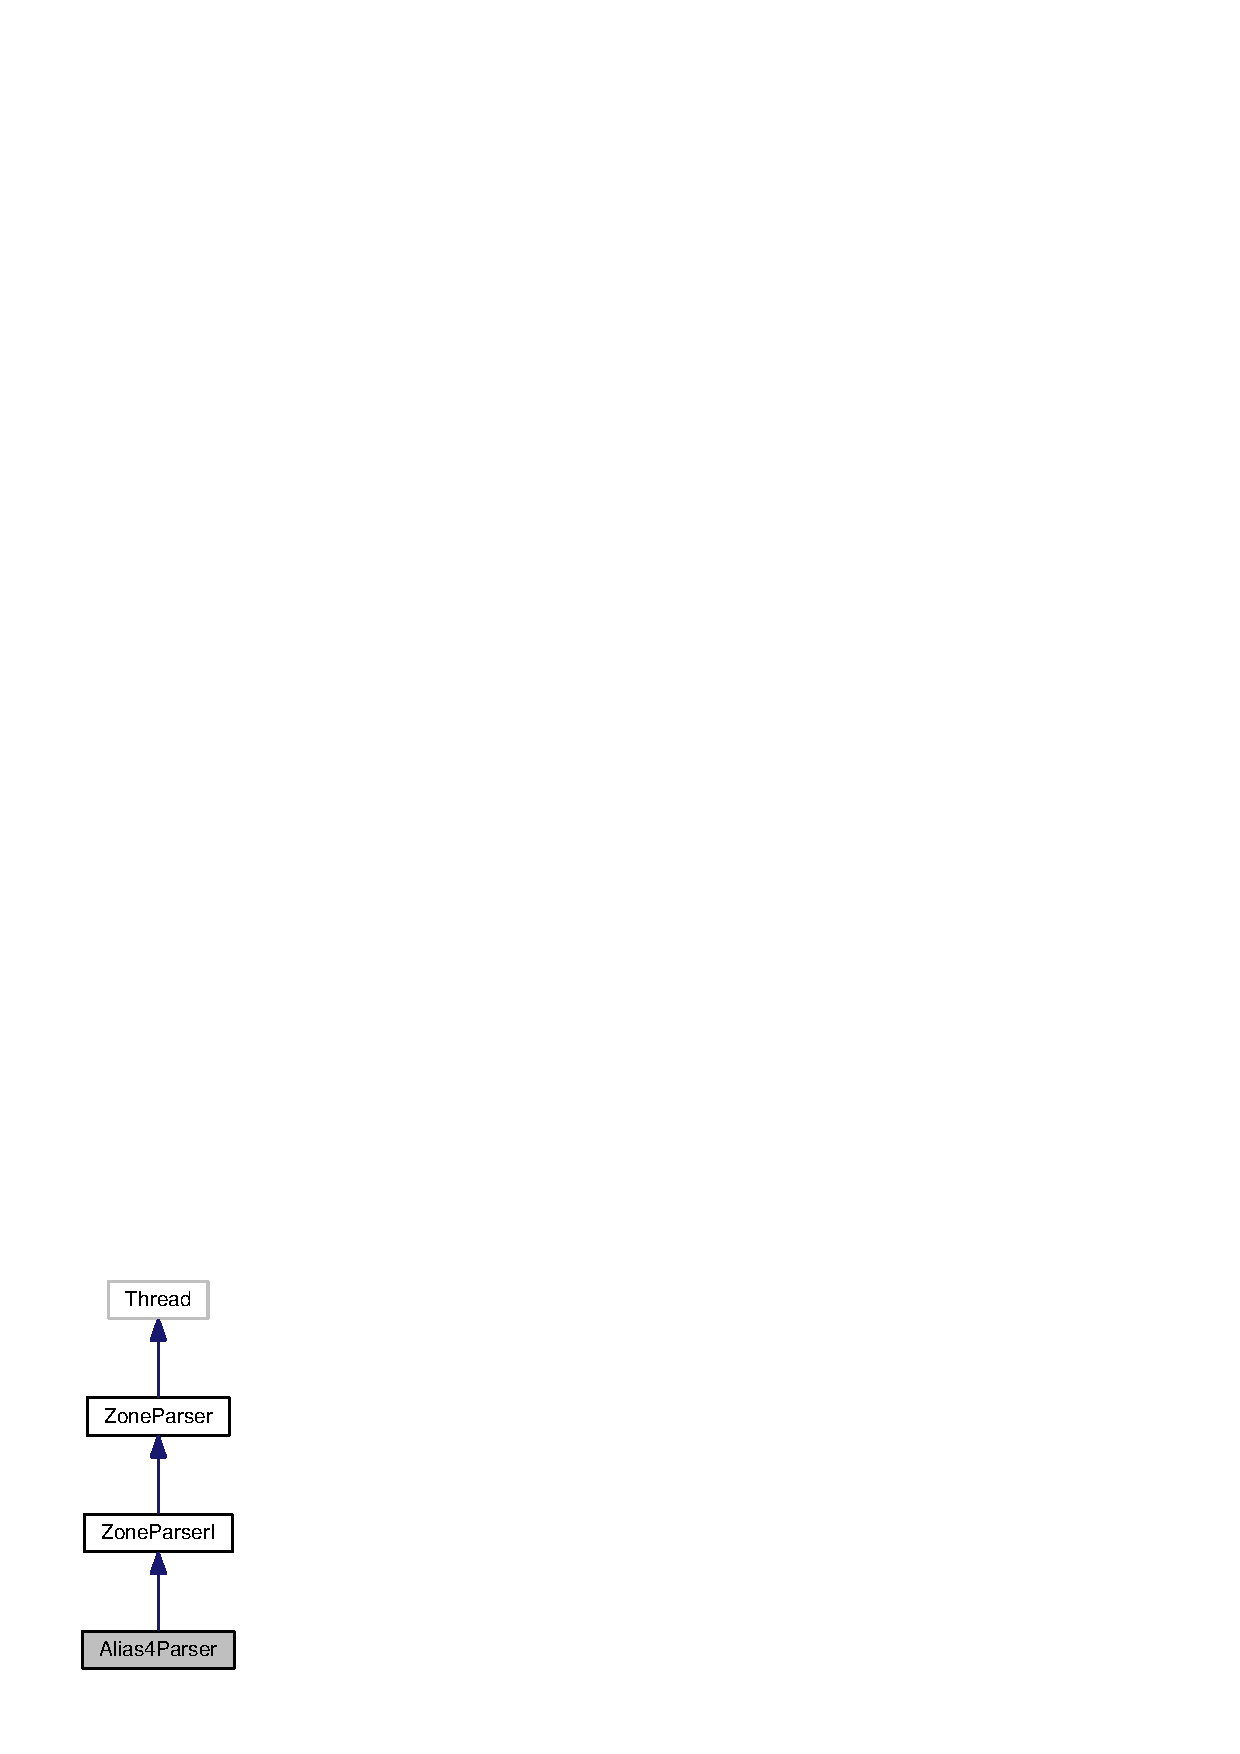
\includegraphics[width=116pt]{classorg_1_1smallfoot_1_1parser_1_1zone_1_1Alias4Parser__inherit__graph}
\end{center}
\end{figure}


Collaboration diagram for Alias4\-Parser\-:\nopagebreak
\begin{figure}[H]
\begin{center}
\leavevmode
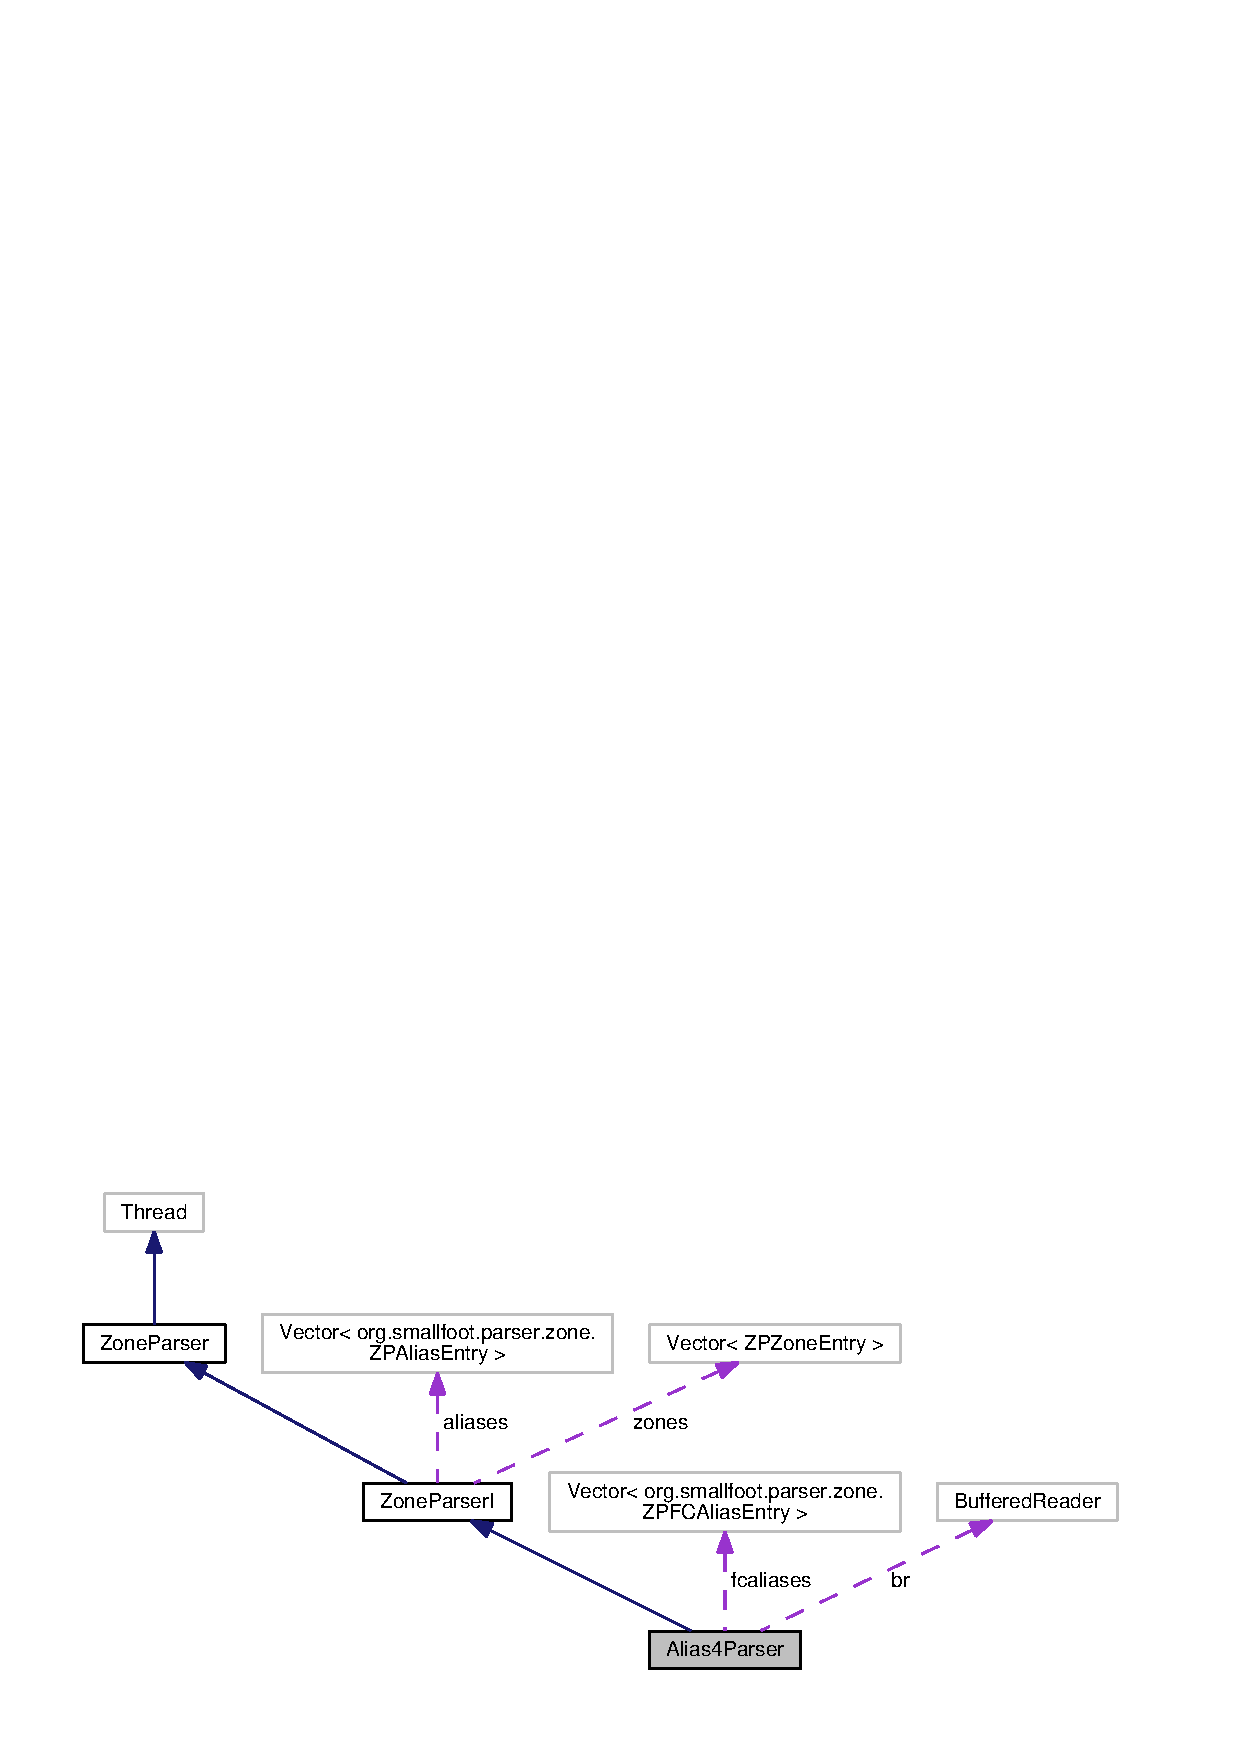
\includegraphics[width=219pt]{classorg_1_1smallfoot_1_1parser_1_1zone_1_1Alias4Parser__coll__graph}
\end{center}
\end{figure}
\subsection*{Public Member Functions}
\begin{DoxyCompactItemize}
\item 
void {\bf set\-Debug} (boolean debug)
\item 
void {\bf set\-Reader} (java.\-io.\-Reader is)
\item 
{\bf Alias4\-Parser} (java.\-util.\-Properties in, boolean debug\-Me)
\item 
void {\bf run} ()
\item 
{\bf Alias4\-Parser} (java.\-io.\-Input\-Stream in)
\begin{DoxyCompactList}\small\item\em Create a parser with a new stream, defaulting to no debug, and verbose Z\-P debug. \end{DoxyCompactList}\item 
{\bf Alias4\-Parser} ()
\begin{DoxyCompactList}\small\item\em Create a parser with a no stream or reader, fairly uncivilized, defaulting to no debug. \end{DoxyCompactList}\item 
{\bf Alias4\-Parser} (java.\-io.\-Input\-Stream in, boolean debug\-Me)
\begin{DoxyCompactList}\small\item\em Create a parser with a new stream. \end{DoxyCompactList}\item 
{\bf Alias4\-Parser} (Reader in, boolean debug\-Me)
\begin{DoxyCompactList}\small\item\em Create a parser, setting the debug to true or false. \end{DoxyCompactList}\end{DoxyCompactItemize}
\subsection*{Static Public Member Functions}
\begin{DoxyCompactItemize}
\item 
static void {\bf main} (String args[$\,$])
\end{DoxyCompactItemize}


\subsection{Detailed Description}


Definition at line 7 of file Alias4\-Parser.\-java.



\subsection{Constructor \& Destructor Documentation}
\index{org\-::smallfoot\-::parser\-::zone\-::\-Alias4\-Parser@{org\-::smallfoot\-::parser\-::zone\-::\-Alias4\-Parser}!Alias4\-Parser@{Alias4\-Parser}}
\index{Alias4\-Parser@{Alias4\-Parser}!org::smallfoot::parser::zone::Alias4Parser@{org\-::smallfoot\-::parser\-::zone\-::\-Alias4\-Parser}}
\subsubsection[{Alias4\-Parser}]{\setlength{\rightskip}{0pt plus 5cm}{\bf Alias4\-Parser} (
\begin{DoxyParamCaption}
\item[{java.\-util.\-Properties}]{in, }
\item[{boolean}]{debug\-Me}
\end{DoxyParamCaption}
)\hspace{0.3cm}{\ttfamily [inline]}}\label{classorg_1_1smallfoot_1_1parser_1_1zone_1_1Alias4Parser_a7b003de53f79832df5f1845e91a48d76}


Definition at line 24 of file Alias4\-Parser.\-java.

\index{org\-::smallfoot\-::parser\-::zone\-::\-Alias4\-Parser@{org\-::smallfoot\-::parser\-::zone\-::\-Alias4\-Parser}!Alias4\-Parser@{Alias4\-Parser}}
\index{Alias4\-Parser@{Alias4\-Parser}!org::smallfoot::parser::zone::Alias4Parser@{org\-::smallfoot\-::parser\-::zone\-::\-Alias4\-Parser}}
\subsubsection[{Alias4\-Parser}]{\setlength{\rightskip}{0pt plus 5cm}{\bf Alias4\-Parser} (
\begin{DoxyParamCaption}
\item[{java.\-io.\-Input\-Stream}]{in}
\end{DoxyParamCaption}
)\hspace{0.3cm}{\ttfamily [inline]}}\label{classorg_1_1smallfoot_1_1parser_1_1zone_1_1Alias4Parser_a298e31048a0168fc5cc4e79abc966fd2}


Create a parser with a new stream, defaulting to no debug, and verbose Z\-P debug. 


\begin{DoxyParams}{Parameters}
{\em in} & Input\-Stream that is the source of bytes to consume \\
\hline
\end{DoxyParams}


Definition at line 71 of file Alias4\-Parser.\-java.

\index{org\-::smallfoot\-::parser\-::zone\-::\-Alias4\-Parser@{org\-::smallfoot\-::parser\-::zone\-::\-Alias4\-Parser}!Alias4\-Parser@{Alias4\-Parser}}
\index{Alias4\-Parser@{Alias4\-Parser}!org::smallfoot::parser::zone::Alias4Parser@{org\-::smallfoot\-::parser\-::zone\-::\-Alias4\-Parser}}
\subsubsection[{Alias4\-Parser}]{\setlength{\rightskip}{0pt plus 5cm}{\bf Alias4\-Parser} (
\begin{DoxyParamCaption}
{}
\end{DoxyParamCaption}
)\hspace{0.3cm}{\ttfamily [inline]}}\label{classorg_1_1smallfoot_1_1parser_1_1zone_1_1Alias4Parser_af385e3c075112d912bb0dad0d9324372}


Create a parser with a no stream or reader, fairly uncivilized, defaulting to no debug. 



Definition at line 80 of file Alias4\-Parser.\-java.



Referenced by Alias4\-Parser.\-main().

\index{org\-::smallfoot\-::parser\-::zone\-::\-Alias4\-Parser@{org\-::smallfoot\-::parser\-::zone\-::\-Alias4\-Parser}!Alias4\-Parser@{Alias4\-Parser}}
\index{Alias4\-Parser@{Alias4\-Parser}!org::smallfoot::parser::zone::Alias4Parser@{org\-::smallfoot\-::parser\-::zone\-::\-Alias4\-Parser}}
\subsubsection[{Alias4\-Parser}]{\setlength{\rightskip}{0pt plus 5cm}{\bf Alias4\-Parser} (
\begin{DoxyParamCaption}
\item[{java.\-io.\-Input\-Stream}]{in, }
\item[{boolean}]{debug\-Me}
\end{DoxyParamCaption}
)\hspace{0.3cm}{\ttfamily [inline]}}\label{classorg_1_1smallfoot_1_1parser_1_1zone_1_1Alias4Parser_a6332334673488c613c5ea2d667b98626}


Create a parser with a new stream. 


\begin{DoxyParams}{Parameters}
{\em in} & Input\-Stream that is the source of bytes to consume \\
\hline
{\em debug\-Me} & true for debugging, false for no debug. \\
\hline
\end{DoxyParams}


Definition at line 92 of file Alias4\-Parser.\-java.

\index{org\-::smallfoot\-::parser\-::zone\-::\-Alias4\-Parser@{org\-::smallfoot\-::parser\-::zone\-::\-Alias4\-Parser}!Alias4\-Parser@{Alias4\-Parser}}
\index{Alias4\-Parser@{Alias4\-Parser}!org::smallfoot::parser::zone::Alias4Parser@{org\-::smallfoot\-::parser\-::zone\-::\-Alias4\-Parser}}
\subsubsection[{Alias4\-Parser}]{\setlength{\rightskip}{0pt plus 5cm}{\bf Alias4\-Parser} (
\begin{DoxyParamCaption}
\item[{Reader}]{in, }
\item[{boolean}]{debug\-Me}
\end{DoxyParamCaption}
)\hspace{0.3cm}{\ttfamily [inline]}}\label{classorg_1_1smallfoot_1_1parser_1_1zone_1_1Alias4Parser_a619525690dfd9b583a9be3eb03fc590a}


Create a parser, setting the debug to true or false. 


\begin{DoxyParams}{Parameters}
{\em in} & Reader that is the source of bytes to consume \\
\hline
{\em debug\-Me} & true for debugging, false for no debug. \\
\hline
\end{DoxyParams}


Definition at line 105 of file Alias4\-Parser.\-java.



References Alias4\-Parser.\-set\-Debug(), and Alias4\-Parser.\-set\-Reader().



Here is the call graph for this function\-:\nopagebreak
\begin{figure}[H]
\begin{center}
\leavevmode
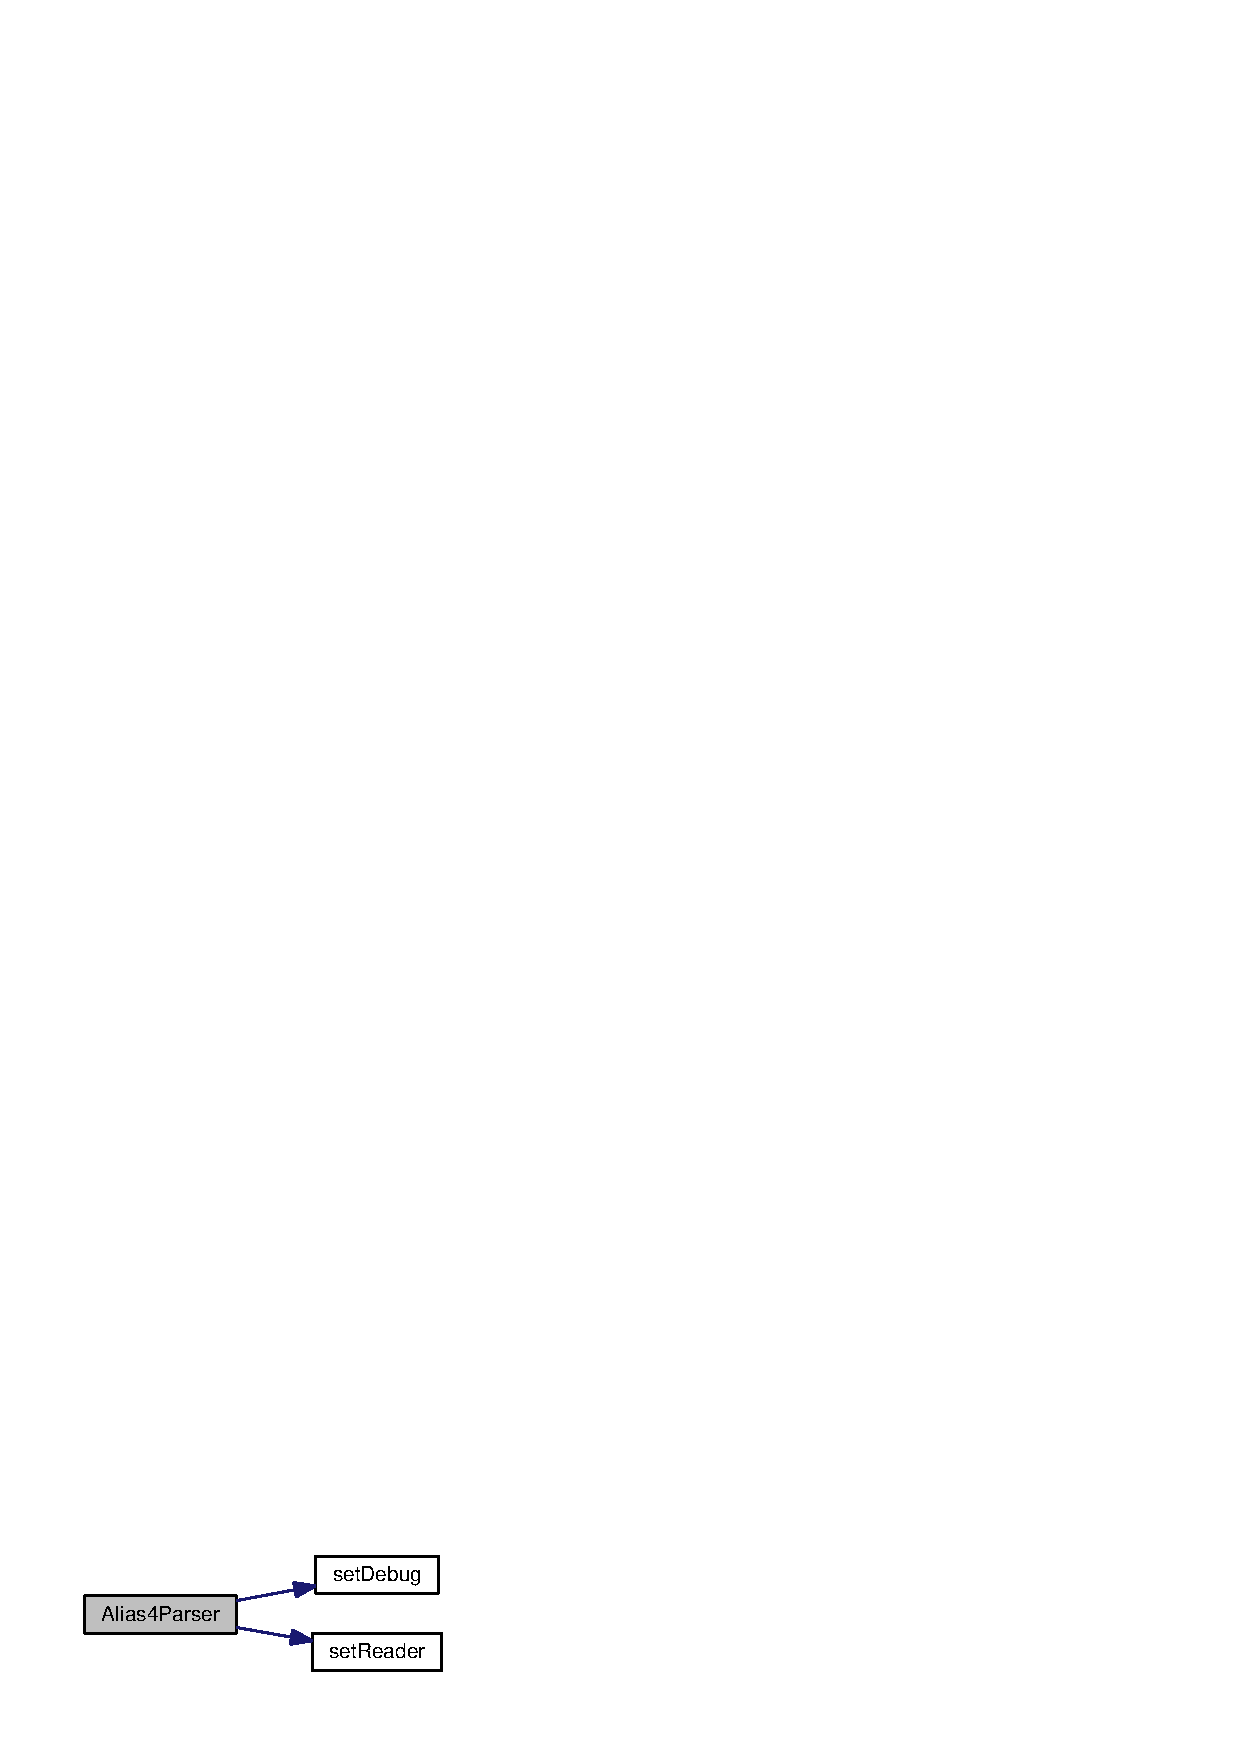
\includegraphics[width=216pt]{classorg_1_1smallfoot_1_1parser_1_1zone_1_1Alias4Parser_a619525690dfd9b583a9be3eb03fc590a_cgraph}
\end{center}
\end{figure}




\subsection{Member Function Documentation}
\index{org\-::smallfoot\-::parser\-::zone\-::\-Alias4\-Parser@{org\-::smallfoot\-::parser\-::zone\-::\-Alias4\-Parser}!main@{main}}
\index{main@{main}!org::smallfoot::parser::zone::Alias4Parser@{org\-::smallfoot\-::parser\-::zone\-::\-Alias4\-Parser}}
\subsubsection[{main}]{\setlength{\rightskip}{0pt plus 5cm}static void main (
\begin{DoxyParamCaption}
\item[{String}]{args[$\,$]}
\end{DoxyParamCaption}
)\hspace{0.3cm}{\ttfamily [inline]}, {\ttfamily [static]}}\label{classorg_1_1smallfoot_1_1parser_1_1zone_1_1Alias4Parser_a75988cf84fc6ee7a2ebff36e363021aa}


Definition at line 113 of file Alias4\-Parser.\-java.



References Alias4\-Parser.\-Alias4\-Parser().



Here is the call graph for this function\-:\nopagebreak
\begin{figure}[H]
\begin{center}
\leavevmode
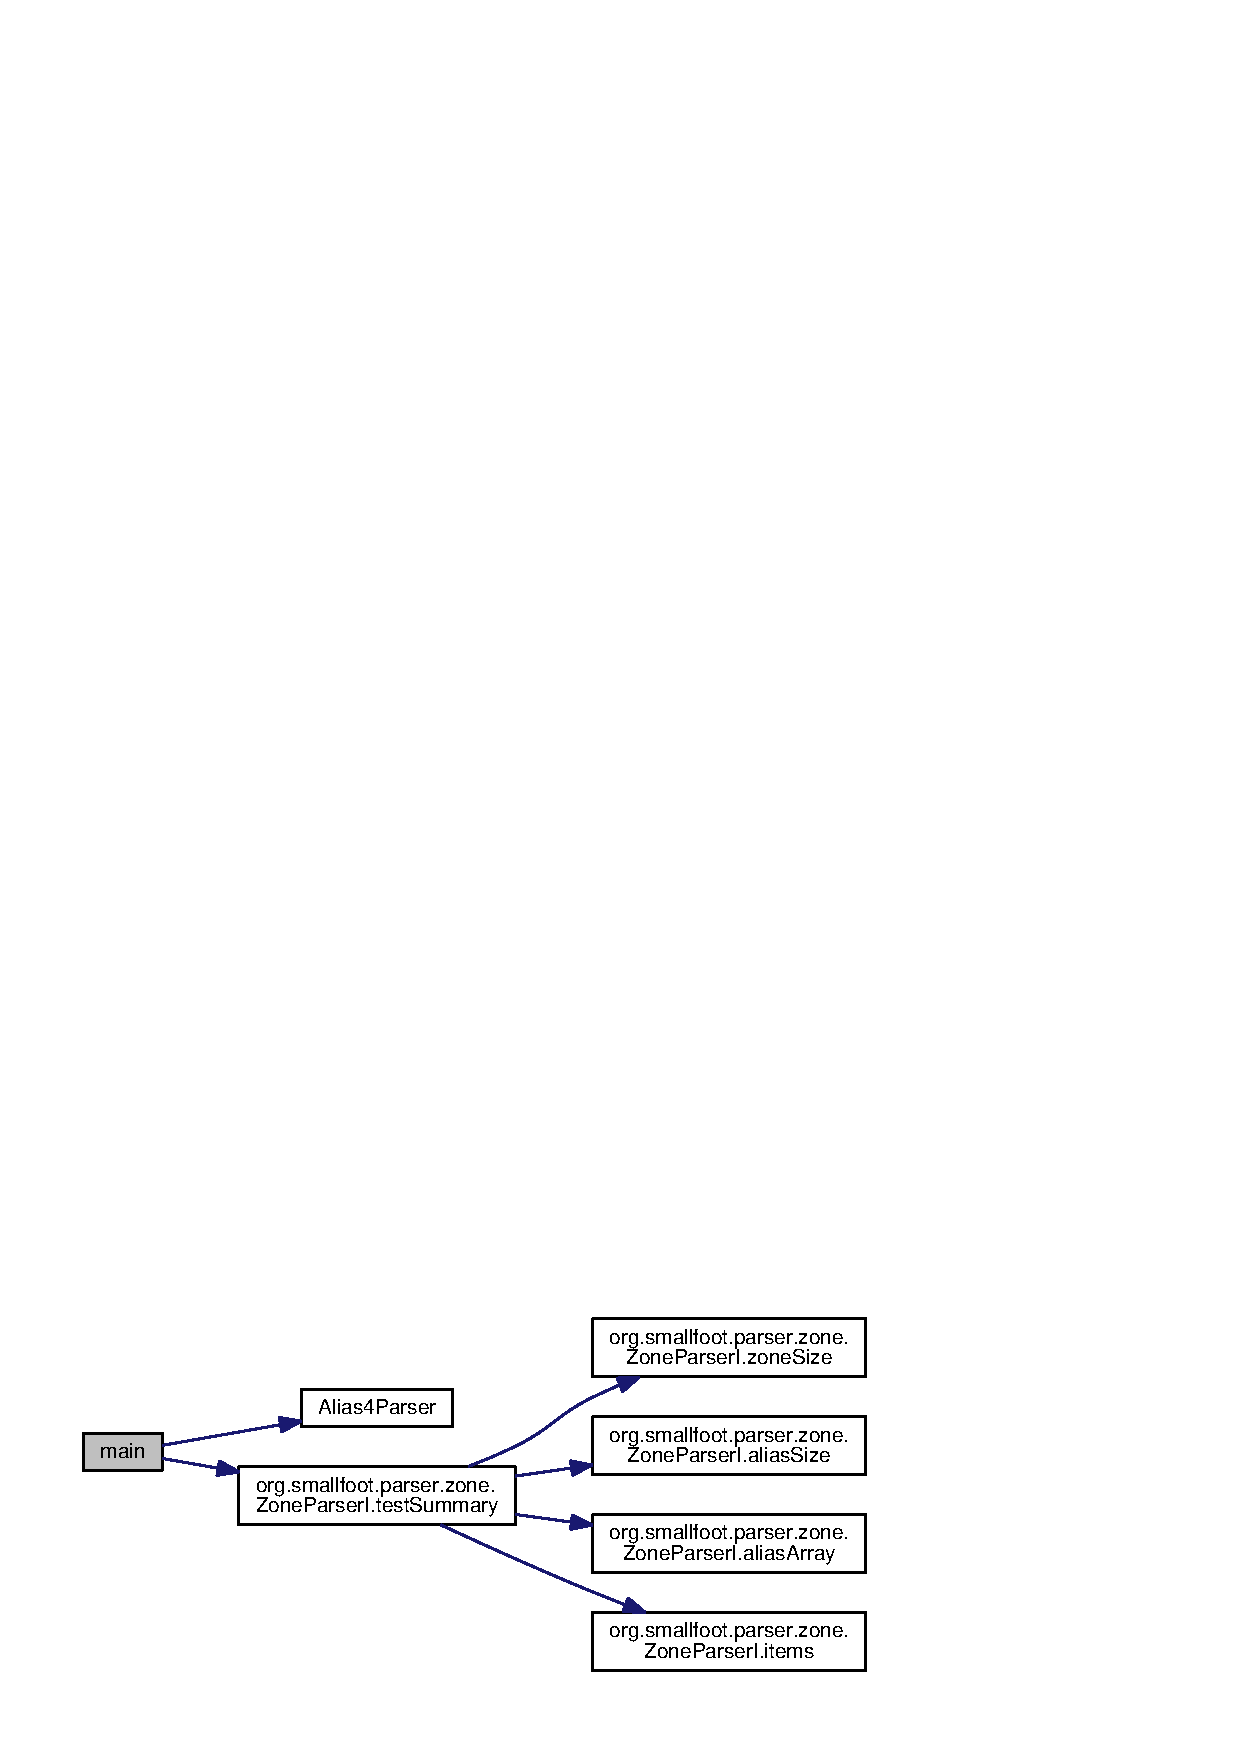
\includegraphics[width=192pt]{classorg_1_1smallfoot_1_1parser_1_1zone_1_1Alias4Parser_a75988cf84fc6ee7a2ebff36e363021aa_cgraph}
\end{center}
\end{figure}


\index{org\-::smallfoot\-::parser\-::zone\-::\-Alias4\-Parser@{org\-::smallfoot\-::parser\-::zone\-::\-Alias4\-Parser}!run@{run}}
\index{run@{run}!org::smallfoot::parser::zone::Alias4Parser@{org\-::smallfoot\-::parser\-::zone\-::\-Alias4\-Parser}}
\subsubsection[{run}]{\setlength{\rightskip}{0pt plus 5cm}void run (
\begin{DoxyParamCaption}
{}
\end{DoxyParamCaption}
)\hspace{0.3cm}{\ttfamily [inline]}}\label{classorg_1_1smallfoot_1_1parser_1_1zone_1_1Alias4Parser_a13a43e6d814de94978c515cb084873b1}


Definition at line 30 of file Alias4\-Parser.\-java.

\index{org\-::smallfoot\-::parser\-::zone\-::\-Alias4\-Parser@{org\-::smallfoot\-::parser\-::zone\-::\-Alias4\-Parser}!set\-Debug@{set\-Debug}}
\index{set\-Debug@{set\-Debug}!org::smallfoot::parser::zone::Alias4Parser@{org\-::smallfoot\-::parser\-::zone\-::\-Alias4\-Parser}}
\subsubsection[{set\-Debug}]{\setlength{\rightskip}{0pt plus 5cm}void set\-Debug (
\begin{DoxyParamCaption}
\item[{boolean}]{debug}
\end{DoxyParamCaption}
)\hspace{0.3cm}{\ttfamily [inline]}}\label{classorg_1_1smallfoot_1_1parser_1_1zone_1_1Alias4Parser_a6c13d260cf71d0554f789c4641a9f18b}


Definition at line 13 of file Alias4\-Parser.\-java.



Referenced by Alias4\-Parser.\-Alias4\-Parser().

\index{org\-::smallfoot\-::parser\-::zone\-::\-Alias4\-Parser@{org\-::smallfoot\-::parser\-::zone\-::\-Alias4\-Parser}!set\-Reader@{set\-Reader}}
\index{set\-Reader@{set\-Reader}!org::smallfoot::parser::zone::Alias4Parser@{org\-::smallfoot\-::parser\-::zone\-::\-Alias4\-Parser}}
\subsubsection[{set\-Reader}]{\setlength{\rightskip}{0pt plus 5cm}void set\-Reader (
\begin{DoxyParamCaption}
\item[{java.\-io.\-Reader}]{is}
\end{DoxyParamCaption}
)\hspace{0.3cm}{\ttfamily [inline]}}\label{classorg_1_1smallfoot_1_1parser_1_1zone_1_1Alias4Parser_aa89f56e94a76b211df071f905e7288ae}


Definition at line 19 of file Alias4\-Parser.\-java.



Referenced by Alias4\-Parser.\-Alias4\-Parser().



The documentation for this class was generated from the following file\-:\begin{DoxyCompactItemize}
\item 
java/{\bf Alias4\-Parser.\-java}\end{DoxyCompactItemize}

\section{Ali\+Show\+Zone\+Parser Class Reference}
\label{classorg_1_1smallfoot_1_1parser_1_1zone_1_1AliShowZoneParser}\index{Ali\+Show\+Zone\+Parser@{Ali\+Show\+Zone\+Parser}}


Inheritance diagram for Ali\+Show\+Zone\+Parser\+:\nopagebreak
\begin{figure}[H]
\begin{center}
\leavevmode
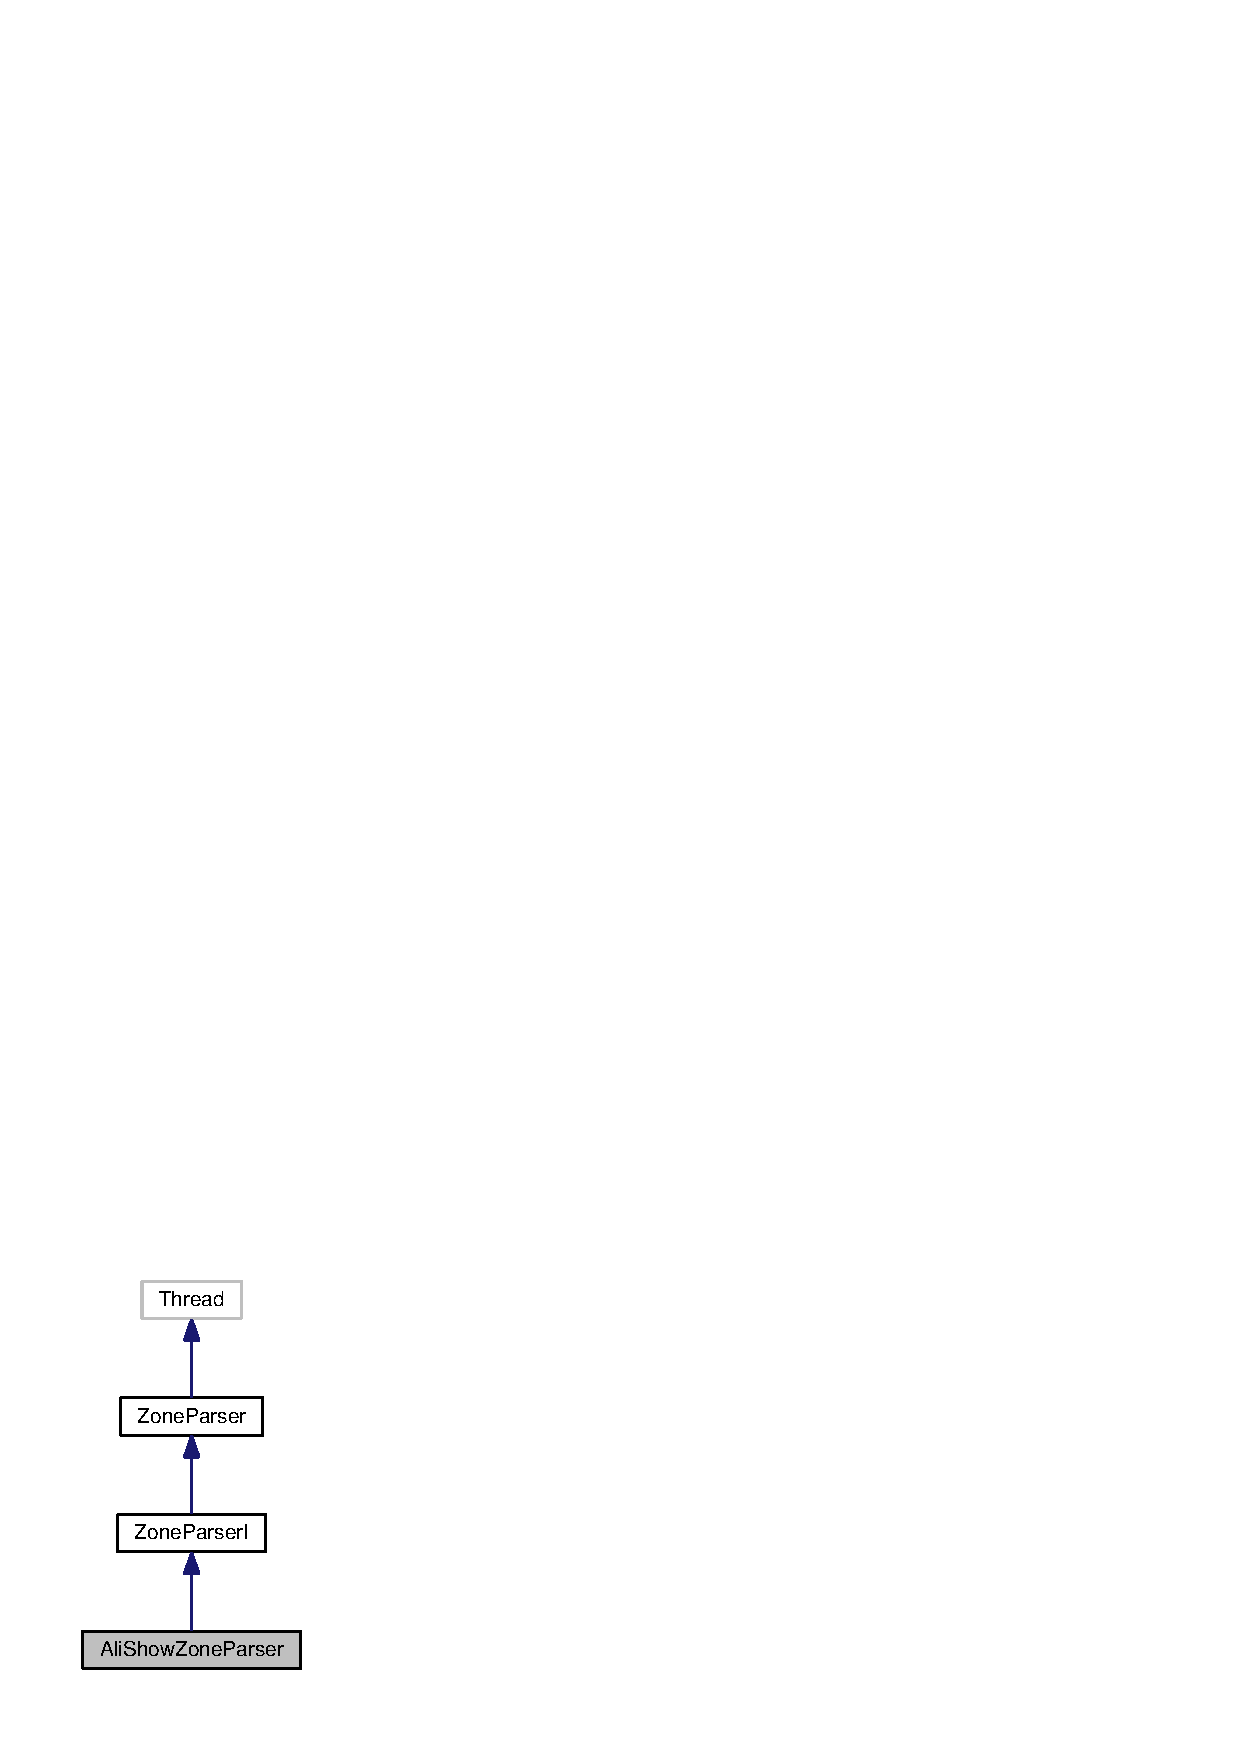
\includegraphics[width=148pt]{classorg_1_1smallfoot_1_1parser_1_1zone_1_1AliShowZoneParser__inherit__graph}
\end{center}
\end{figure}


Collaboration diagram for Ali\+Show\+Zone\+Parser\+:
\nopagebreak
\begin{figure}[H]
\begin{center}
\leavevmode
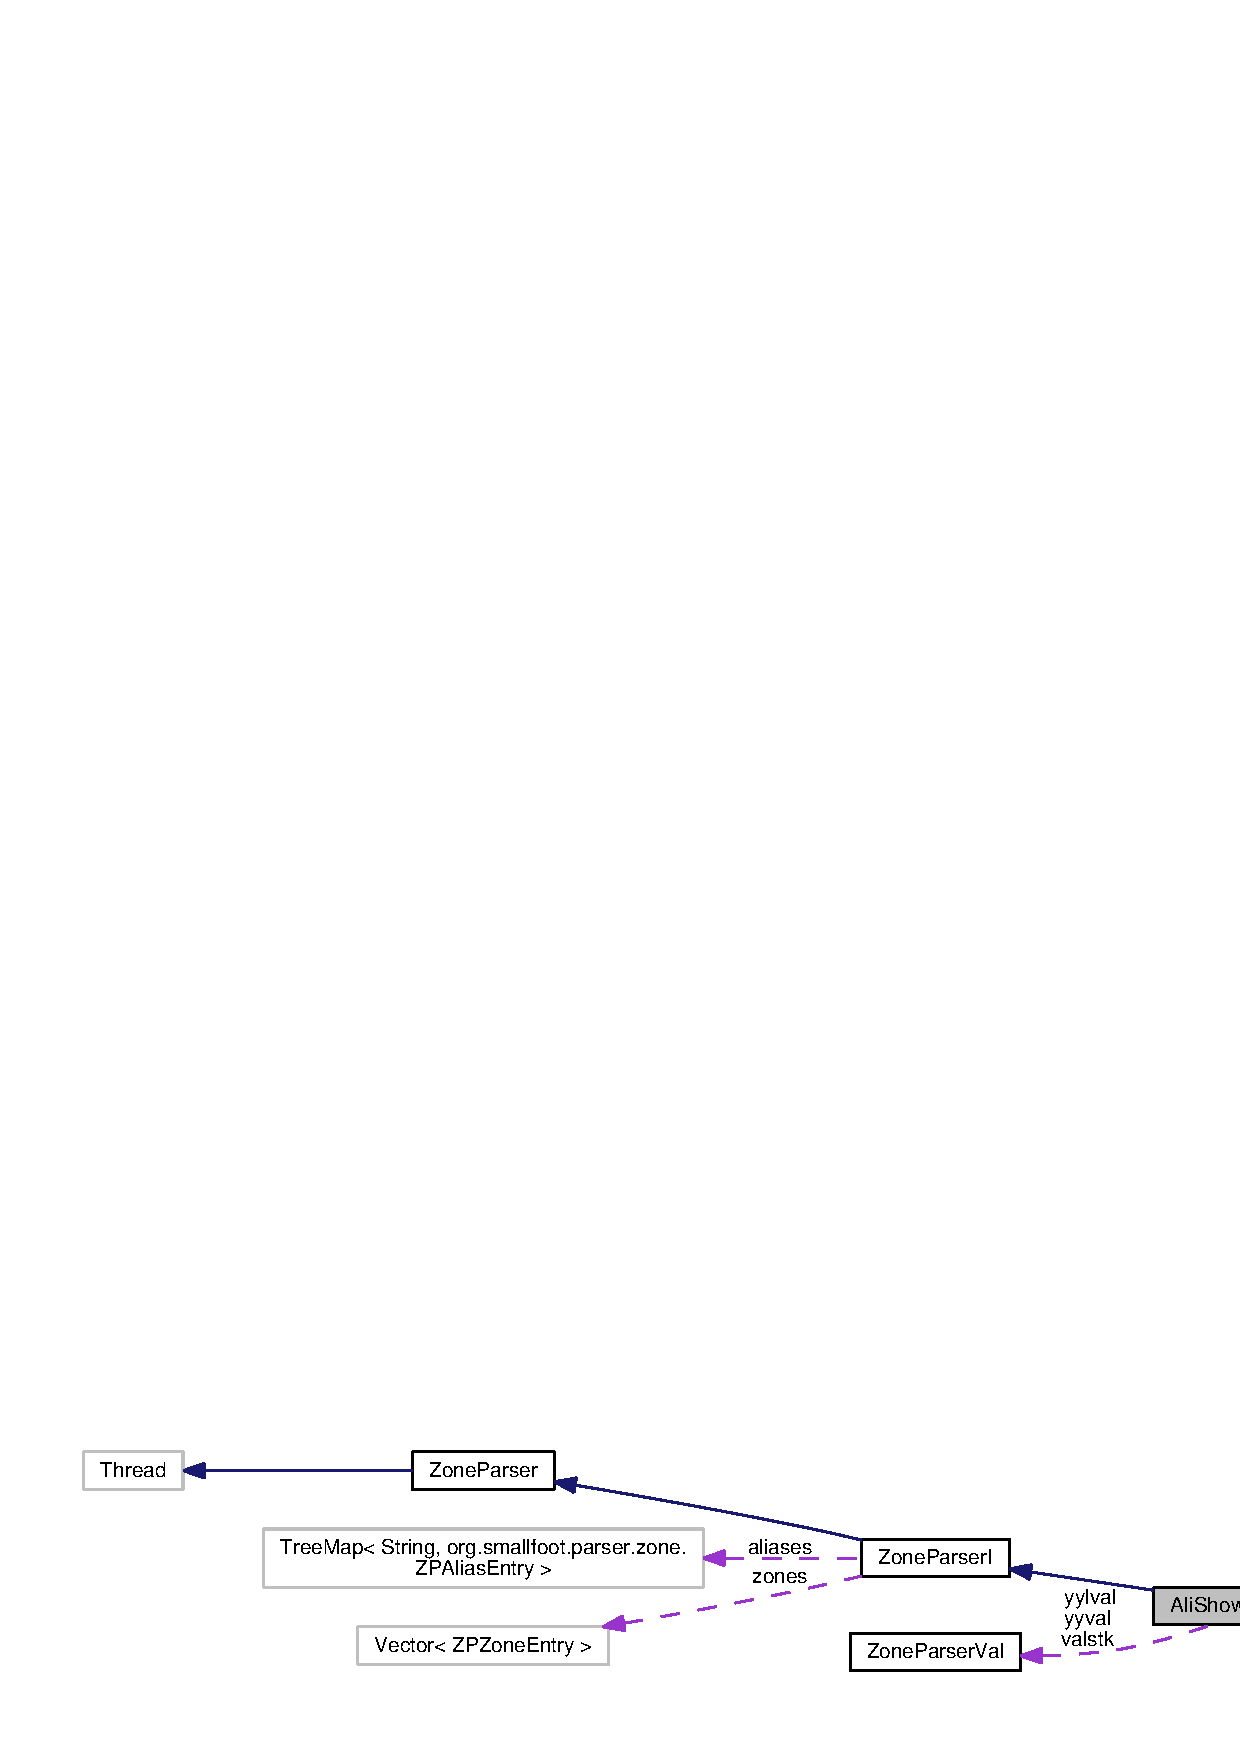
\includegraphics[width=350pt]{classorg_1_1smallfoot_1_1parser_1_1zone_1_1AliShowZoneParser__coll__graph}
\end{center}
\end{figure}
\subsection*{Public Member Functions}
\begin{DoxyCompactItemize}
\item 
void {\bf parse} ()
\item 
void {\bf set\+Reader} (Reader in)
\item 
void {\bf run} ()
\item 
void {\bf set\+Debug} (boolean debug)
\item 
{\bf Ali\+Show\+Zone\+Parser} (Input\+Stream in, boolean debug\+Me)
\item 
{\bf Ali\+Show\+Zone\+Parser} (java.\+util.\+Properties in)
\end{DoxyCompactItemize}
\subsection*{Static Public Member Functions}
\begin{DoxyCompactItemize}
\item 
static void {\bf main} (String args[$\,$])
\end{DoxyCompactItemize}
\subsection*{Static Public Attributes}
\begin{DoxyCompactItemize}
\item 
static final short {\bf Z\+O\+N\+E} =257
\item 
static final short {\bf A\+L\+I\+A\+S} =258
\item 
static final short {\bf A\+L\+I\+Z\+O\+N\+E\+S\+H\+O\+W\+C\+O\+M\+M\+A\+N\+D} =259
\item 
static final short {\bf A\+L\+P\+H\+A\+N\+U\+M} =260
\item 
static final short {\bf D\+E\+F\+I\+N\+E\+D} =261
\item 
static final short {\bf E\+F\+F\+E\+C\+T\+I\+V\+E} =262
\item 
static final short {\bf C\+O\+N\+F\+I\+G\+U\+R\+A\+T\+I\+O\+N} =263
\item 
static final short {\bf C\+F\+G} =264
\item 
static final short {\bf H\+A\+R\+D\+Z\+O\+N\+E} =265
\item 
static final short {\bf H} =266
\item 
static final short {\bf O\+P\+E\+N\+P\+A\+R\+E\+N} =267
\item 
static final short {\bf C\+L\+O\+S\+E\+P\+A\+R\+E\+N} =268
\item 
static final short {\bf Y\+Y\+E\+R\+R\+C\+O\+D\+E} =256
\end{DoxyCompactItemize}


\subsection{Detailed Description}


Definition at line 116 of file Ali\+Show\+Zone\+Parser.\+java.



\subsection{Constructor \& Destructor Documentation}
\index{org\+::smallfoot\+::parser\+::zone\+::\+Ali\+Show\+Zone\+Parser@{org\+::smallfoot\+::parser\+::zone\+::\+Ali\+Show\+Zone\+Parser}!Ali\+Show\+Zone\+Parser@{Ali\+Show\+Zone\+Parser}}
\index{Ali\+Show\+Zone\+Parser@{Ali\+Show\+Zone\+Parser}!org\+::smallfoot\+::parser\+::zone\+::\+Ali\+Show\+Zone\+Parser@{org\+::smallfoot\+::parser\+::zone\+::\+Ali\+Show\+Zone\+Parser}}
\subsubsection[{Ali\+Show\+Zone\+Parser}]{\setlength{\rightskip}{0pt plus 5cm}{\bf Ali\+Show\+Zone\+Parser} (
\begin{DoxyParamCaption}
\item[{Input\+Stream}]{in, }
\item[{boolean}]{debug\+Me}
\end{DoxyParamCaption}
)\hspace{0.3cm}{\ttfamily [inline]}}\label{classorg_1_1smallfoot_1_1parser_1_1zone_1_1AliShowZoneParser_a5e03a31a37a94bc78cf316ea5a3ee575}


Definition at line 592 of file Ali\+Show\+Zone\+Parser.\+java.



Referenced by Ali\+Show\+Zone\+Parser.\+main().

\index{org\+::smallfoot\+::parser\+::zone\+::\+Ali\+Show\+Zone\+Parser@{org\+::smallfoot\+::parser\+::zone\+::\+Ali\+Show\+Zone\+Parser}!Ali\+Show\+Zone\+Parser@{Ali\+Show\+Zone\+Parser}}
\index{Ali\+Show\+Zone\+Parser@{Ali\+Show\+Zone\+Parser}!org\+::smallfoot\+::parser\+::zone\+::\+Ali\+Show\+Zone\+Parser@{org\+::smallfoot\+::parser\+::zone\+::\+Ali\+Show\+Zone\+Parser}}
\subsubsection[{Ali\+Show\+Zone\+Parser}]{\setlength{\rightskip}{0pt plus 5cm}{\bf Ali\+Show\+Zone\+Parser} (
\begin{DoxyParamCaption}
\item[{java.\+util.\+Properties}]{in}
\end{DoxyParamCaption}
)\hspace{0.3cm}{\ttfamily [inline]}}\label{classorg_1_1smallfoot_1_1parser_1_1zone_1_1AliShowZoneParser_a17b50844ec3130260c2258a3a2d78e08}


Definition at line 594 of file Ali\+Show\+Zone\+Parser.\+java.



\subsection{Member Function Documentation}
\index{org\+::smallfoot\+::parser\+::zone\+::\+Ali\+Show\+Zone\+Parser@{org\+::smallfoot\+::parser\+::zone\+::\+Ali\+Show\+Zone\+Parser}!main@{main}}
\index{main@{main}!org\+::smallfoot\+::parser\+::zone\+::\+Ali\+Show\+Zone\+Parser@{org\+::smallfoot\+::parser\+::zone\+::\+Ali\+Show\+Zone\+Parser}}
\subsubsection[{main}]{\setlength{\rightskip}{0pt plus 5cm}static void main (
\begin{DoxyParamCaption}
\item[{String}]{args[$\,$]}
\end{DoxyParamCaption}
)\hspace{0.3cm}{\ttfamily [inline]}, {\ttfamily [static]}}\label{classorg_1_1smallfoot_1_1parser_1_1zone_1_1AliShowZoneParser_a75988cf84fc6ee7a2ebff36e363021aa}


Definition at line 596 of file Ali\+Show\+Zone\+Parser.\+java.



References Ali\+Show\+Zone\+Parser.\+Ali\+Show\+Zone\+Parser(), and Zone\+Parser\+I.\+test\+Summary().



Here is the call graph for this function\+:\nopagebreak
\begin{figure}[H]
\begin{center}
\leavevmode
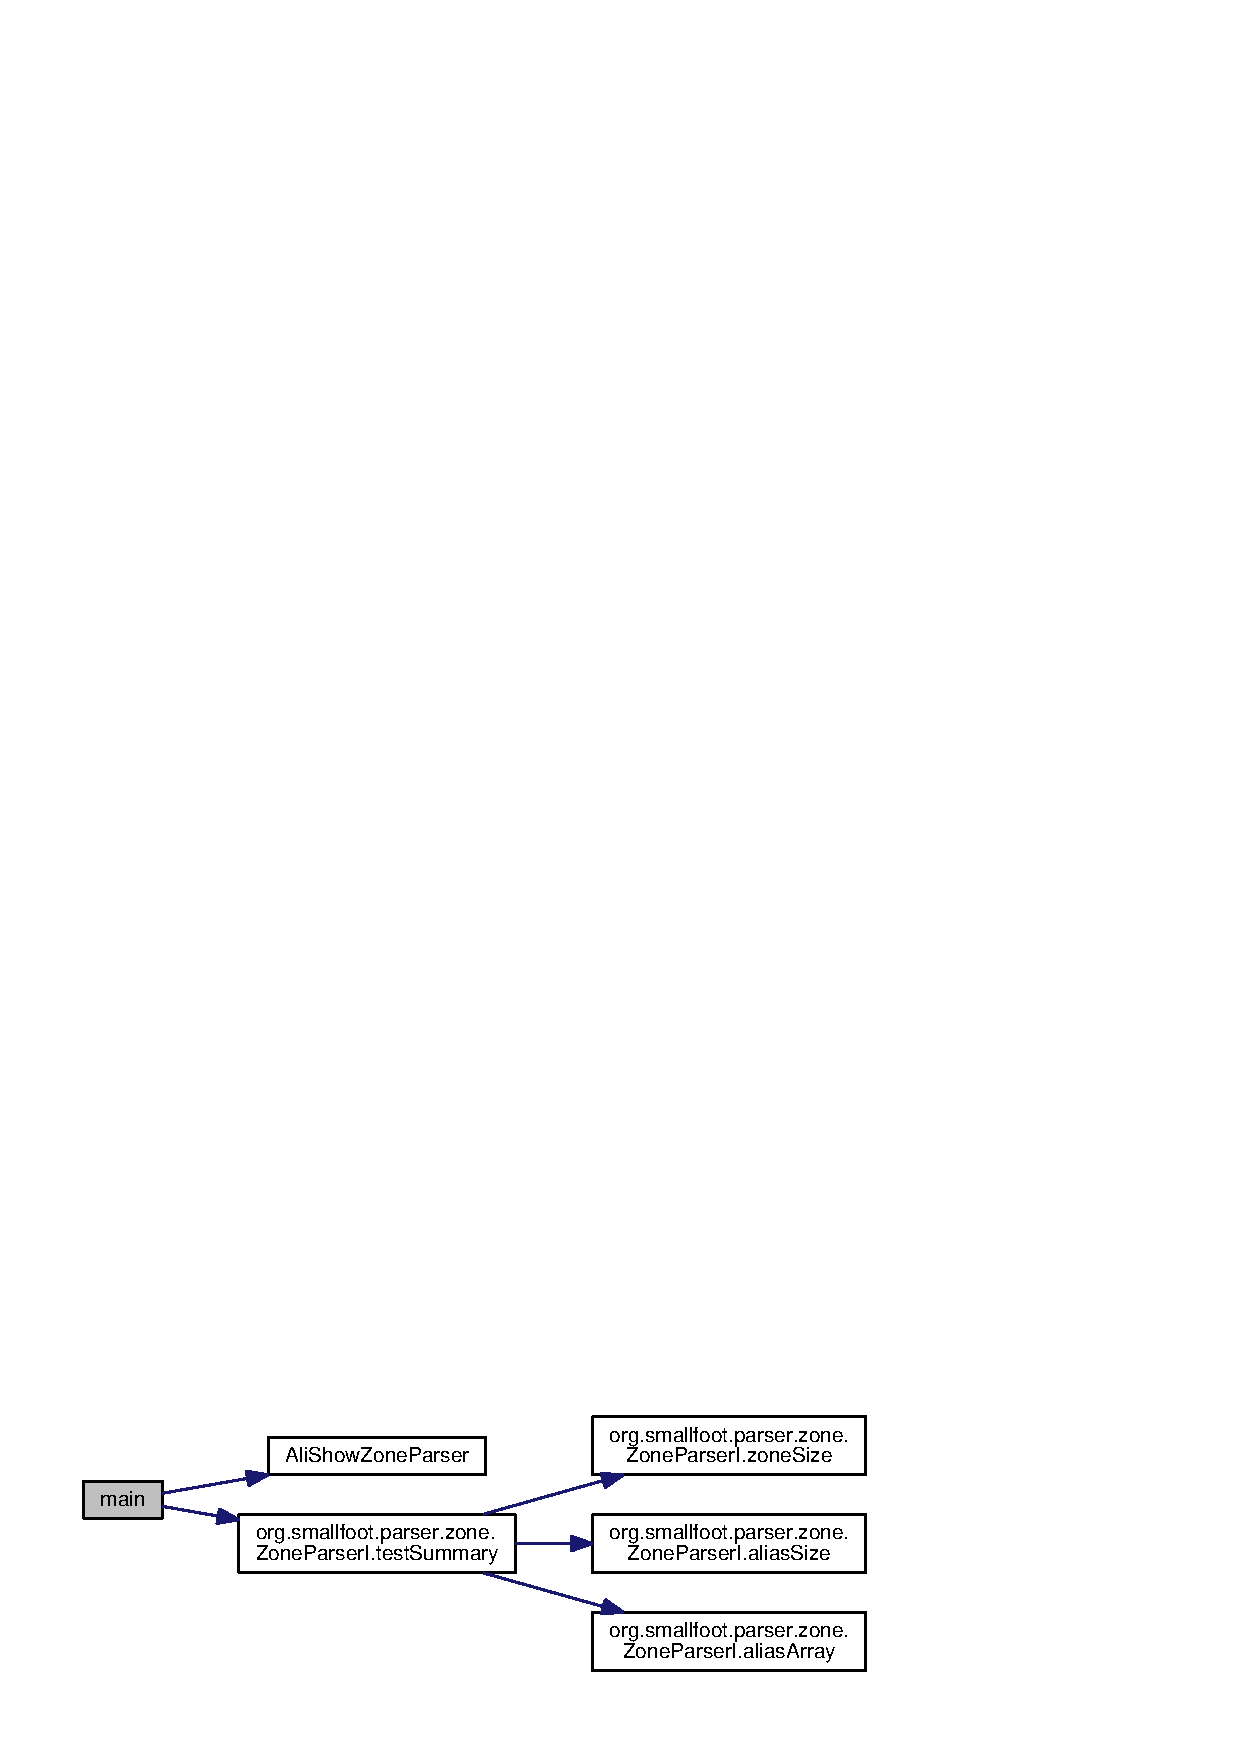
\includegraphics[width=350pt]{classorg_1_1smallfoot_1_1parser_1_1zone_1_1AliShowZoneParser_a75988cf84fc6ee7a2ebff36e363021aa_cgraph}
\end{center}
\end{figure}


\index{org\+::smallfoot\+::parser\+::zone\+::\+Ali\+Show\+Zone\+Parser@{org\+::smallfoot\+::parser\+::zone\+::\+Ali\+Show\+Zone\+Parser}!parse@{parse}}
\index{parse@{parse}!org\+::smallfoot\+::parser\+::zone\+::\+Ali\+Show\+Zone\+Parser@{org\+::smallfoot\+::parser\+::zone\+::\+Ali\+Show\+Zone\+Parser}}
\subsubsection[{parse}]{\setlength{\rightskip}{0pt plus 5cm}void parse (
\begin{DoxyParamCaption}
{}
\end{DoxyParamCaption}
)\hspace{0.3cm}{\ttfamily [inline]}}\label{classorg_1_1smallfoot_1_1parser_1_1zone_1_1AliShowZoneParser_ad7c704b34912678d95c13243cacf9d7f}


Definition at line 532 of file Ali\+Show\+Zone\+Parser.\+java.

\index{org\+::smallfoot\+::parser\+::zone\+::\+Ali\+Show\+Zone\+Parser@{org\+::smallfoot\+::parser\+::zone\+::\+Ali\+Show\+Zone\+Parser}!run@{run}}
\index{run@{run}!org\+::smallfoot\+::parser\+::zone\+::\+Ali\+Show\+Zone\+Parser@{org\+::smallfoot\+::parser\+::zone\+::\+Ali\+Show\+Zone\+Parser}}
\subsubsection[{run}]{\setlength{\rightskip}{0pt plus 5cm}void run (
\begin{DoxyParamCaption}
{}
\end{DoxyParamCaption}
)\hspace{0.3cm}{\ttfamily [inline]}}\label{classorg_1_1smallfoot_1_1parser_1_1zone_1_1AliShowZoneParser_a13a43e6d814de94978c515cb084873b1}


Definition at line 577 of file Ali\+Show\+Zone\+Parser.\+java.



References Ali\+Show\+Zone\+Parser.\+set\+Debug().



Here is the call graph for this function\+:\nopagebreak
\begin{figure}[H]
\begin{center}
\leavevmode
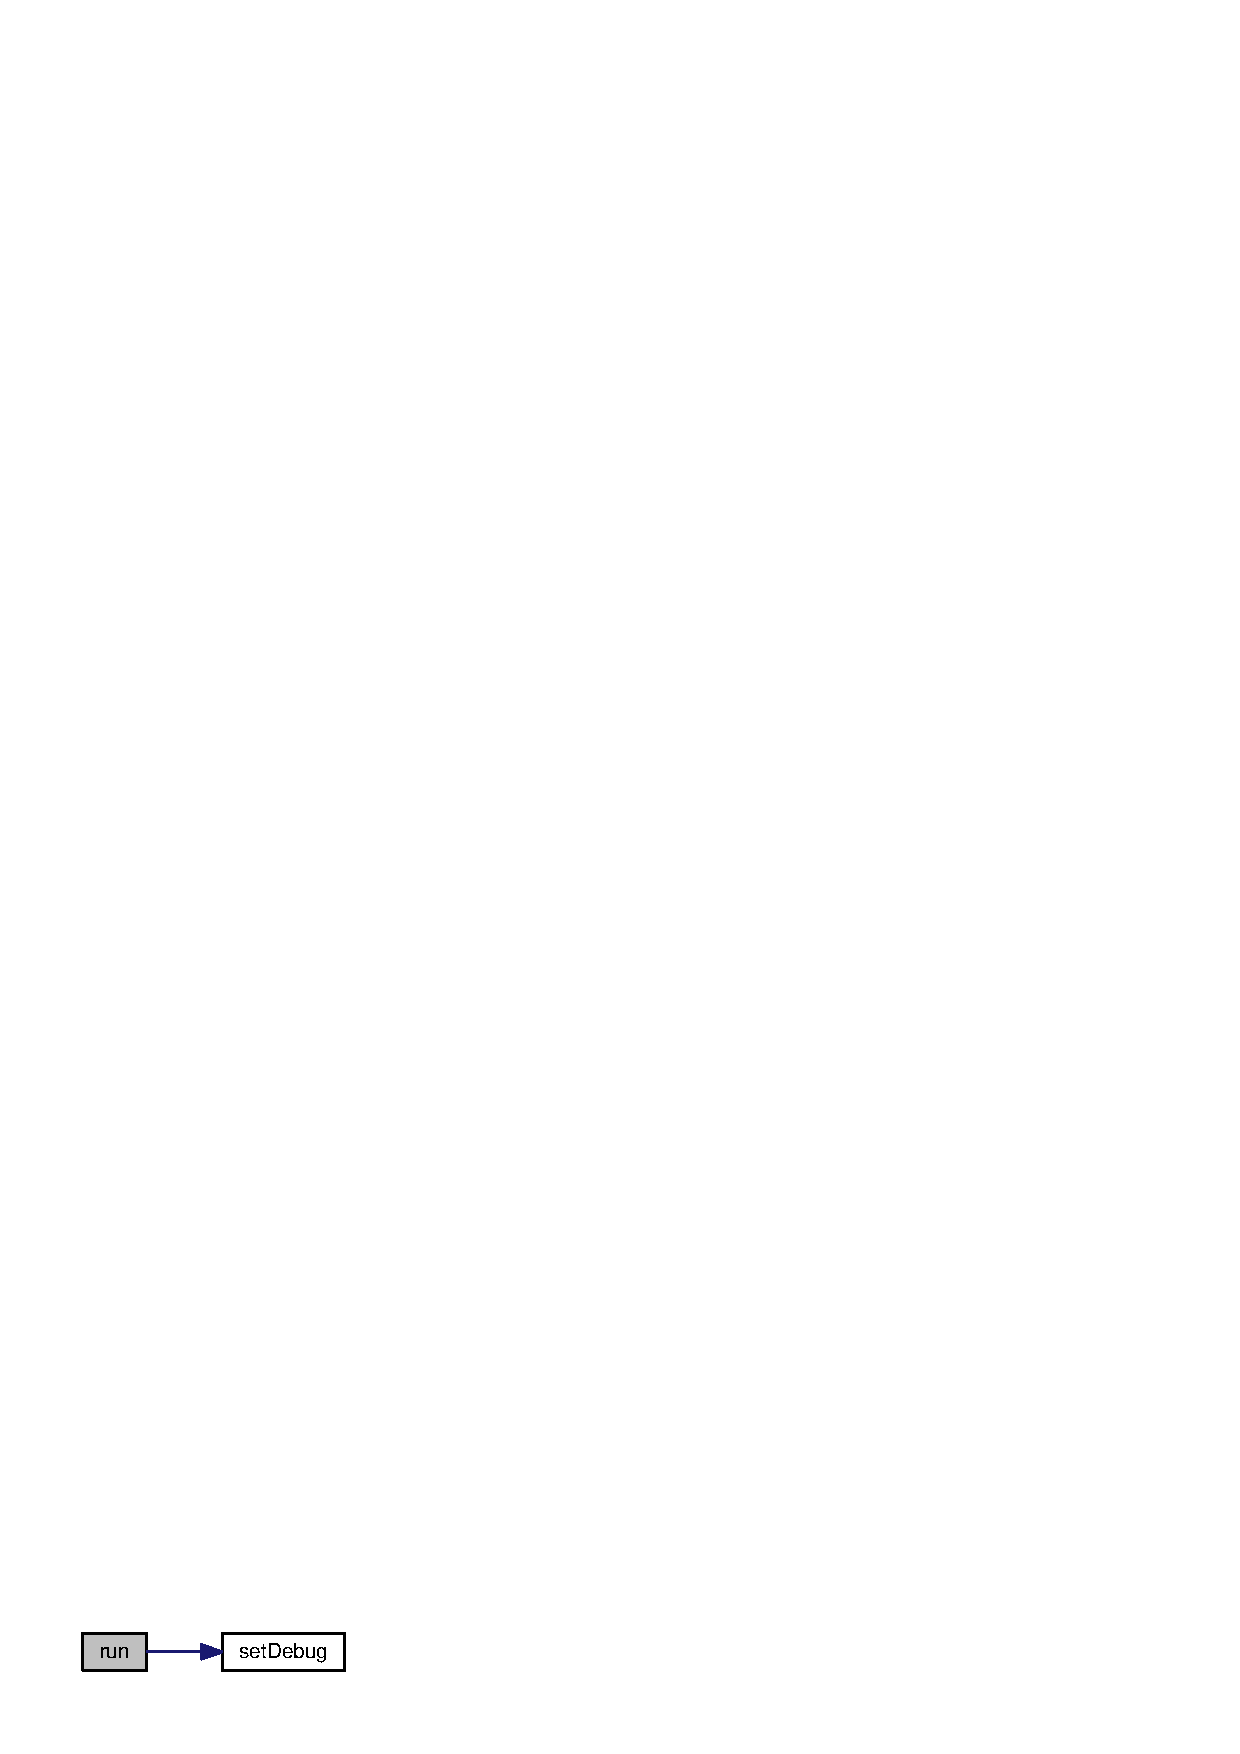
\includegraphics[width=170pt]{classorg_1_1smallfoot_1_1parser_1_1zone_1_1AliShowZoneParser_a13a43e6d814de94978c515cb084873b1_cgraph}
\end{center}
\end{figure}


\index{org\+::smallfoot\+::parser\+::zone\+::\+Ali\+Show\+Zone\+Parser@{org\+::smallfoot\+::parser\+::zone\+::\+Ali\+Show\+Zone\+Parser}!set\+Debug@{set\+Debug}}
\index{set\+Debug@{set\+Debug}!org\+::smallfoot\+::parser\+::zone\+::\+Ali\+Show\+Zone\+Parser@{org\+::smallfoot\+::parser\+::zone\+::\+Ali\+Show\+Zone\+Parser}}
\subsubsection[{set\+Debug}]{\setlength{\rightskip}{0pt plus 5cm}void set\+Debug (
\begin{DoxyParamCaption}
\item[{boolean}]{debug}
\end{DoxyParamCaption}
)\hspace{0.3cm}{\ttfamily [inline]}}\label{classorg_1_1smallfoot_1_1parser_1_1zone_1_1AliShowZoneParser_a6c13d260cf71d0554f789c4641a9f18b}


Definition at line 590 of file Ali\+Show\+Zone\+Parser.\+java.



Referenced by Ali\+Show\+Zone\+Parser.\+run().

\index{org\+::smallfoot\+::parser\+::zone\+::\+Ali\+Show\+Zone\+Parser@{org\+::smallfoot\+::parser\+::zone\+::\+Ali\+Show\+Zone\+Parser}!set\+Reader@{set\+Reader}}
\index{set\+Reader@{set\+Reader}!org\+::smallfoot\+::parser\+::zone\+::\+Ali\+Show\+Zone\+Parser@{org\+::smallfoot\+::parser\+::zone\+::\+Ali\+Show\+Zone\+Parser}}
\subsubsection[{set\+Reader}]{\setlength{\rightskip}{0pt plus 5cm}void set\+Reader (
\begin{DoxyParamCaption}
\item[{Reader}]{in}
\end{DoxyParamCaption}
)\hspace{0.3cm}{\ttfamily [inline]}}\label{classorg_1_1smallfoot_1_1parser_1_1zone_1_1AliShowZoneParser_a5deab139f9ad4072e1a497c5cccda0ea}


Definition at line 544 of file Ali\+Show\+Zone\+Parser.\+java.



\subsection{Field Documentation}
\index{org\+::smallfoot\+::parser\+::zone\+::\+Ali\+Show\+Zone\+Parser@{org\+::smallfoot\+::parser\+::zone\+::\+Ali\+Show\+Zone\+Parser}!A\+L\+I\+A\+S@{A\+L\+I\+A\+S}}
\index{A\+L\+I\+A\+S@{A\+L\+I\+A\+S}!org\+::smallfoot\+::parser\+::zone\+::\+Ali\+Show\+Zone\+Parser@{org\+::smallfoot\+::parser\+::zone\+::\+Ali\+Show\+Zone\+Parser}}
\subsubsection[{A\+L\+I\+A\+S}]{\setlength{\rightskip}{0pt plus 5cm}final short A\+L\+I\+A\+S =258\hspace{0.3cm}{\ttfamily [static]}}\label{classorg_1_1smallfoot_1_1parser_1_1zone_1_1AliShowZoneParser_abb724776f23235ae5f3a3be5505b18bb}


Definition at line 242 of file Ali\+Show\+Zone\+Parser.\+java.

\index{org\+::smallfoot\+::parser\+::zone\+::\+Ali\+Show\+Zone\+Parser@{org\+::smallfoot\+::parser\+::zone\+::\+Ali\+Show\+Zone\+Parser}!A\+L\+I\+Z\+O\+N\+E\+S\+H\+O\+W\+C\+O\+M\+M\+A\+N\+D@{A\+L\+I\+Z\+O\+N\+E\+S\+H\+O\+W\+C\+O\+M\+M\+A\+N\+D}}
\index{A\+L\+I\+Z\+O\+N\+E\+S\+H\+O\+W\+C\+O\+M\+M\+A\+N\+D@{A\+L\+I\+Z\+O\+N\+E\+S\+H\+O\+W\+C\+O\+M\+M\+A\+N\+D}!org\+::smallfoot\+::parser\+::zone\+::\+Ali\+Show\+Zone\+Parser@{org\+::smallfoot\+::parser\+::zone\+::\+Ali\+Show\+Zone\+Parser}}
\subsubsection[{A\+L\+I\+Z\+O\+N\+E\+S\+H\+O\+W\+C\+O\+M\+M\+A\+N\+D}]{\setlength{\rightskip}{0pt plus 5cm}final short A\+L\+I\+Z\+O\+N\+E\+S\+H\+O\+W\+C\+O\+M\+M\+A\+N\+D =259\hspace{0.3cm}{\ttfamily [static]}}\label{classorg_1_1smallfoot_1_1parser_1_1zone_1_1AliShowZoneParser_a51a80cdf90fbf1f9a6376820fa39f92b}


Definition at line 243 of file Ali\+Show\+Zone\+Parser.\+java.

\index{org\+::smallfoot\+::parser\+::zone\+::\+Ali\+Show\+Zone\+Parser@{org\+::smallfoot\+::parser\+::zone\+::\+Ali\+Show\+Zone\+Parser}!A\+L\+P\+H\+A\+N\+U\+M@{A\+L\+P\+H\+A\+N\+U\+M}}
\index{A\+L\+P\+H\+A\+N\+U\+M@{A\+L\+P\+H\+A\+N\+U\+M}!org\+::smallfoot\+::parser\+::zone\+::\+Ali\+Show\+Zone\+Parser@{org\+::smallfoot\+::parser\+::zone\+::\+Ali\+Show\+Zone\+Parser}}
\subsubsection[{A\+L\+P\+H\+A\+N\+U\+M}]{\setlength{\rightskip}{0pt plus 5cm}final short A\+L\+P\+H\+A\+N\+U\+M =260\hspace{0.3cm}{\ttfamily [static]}}\label{classorg_1_1smallfoot_1_1parser_1_1zone_1_1AliShowZoneParser_afa1bd945463851953be939c8793faf70}


Definition at line 244 of file Ali\+Show\+Zone\+Parser.\+java.

\index{org\+::smallfoot\+::parser\+::zone\+::\+Ali\+Show\+Zone\+Parser@{org\+::smallfoot\+::parser\+::zone\+::\+Ali\+Show\+Zone\+Parser}!C\+F\+G@{C\+F\+G}}
\index{C\+F\+G@{C\+F\+G}!org\+::smallfoot\+::parser\+::zone\+::\+Ali\+Show\+Zone\+Parser@{org\+::smallfoot\+::parser\+::zone\+::\+Ali\+Show\+Zone\+Parser}}
\subsubsection[{C\+F\+G}]{\setlength{\rightskip}{0pt plus 5cm}final short C\+F\+G =264\hspace{0.3cm}{\ttfamily [static]}}\label{classorg_1_1smallfoot_1_1parser_1_1zone_1_1AliShowZoneParser_a72139940d21d763668f7f4cc6588b9f4}


Definition at line 248 of file Ali\+Show\+Zone\+Parser.\+java.

\index{org\+::smallfoot\+::parser\+::zone\+::\+Ali\+Show\+Zone\+Parser@{org\+::smallfoot\+::parser\+::zone\+::\+Ali\+Show\+Zone\+Parser}!C\+L\+O\+S\+E\+P\+A\+R\+E\+N@{C\+L\+O\+S\+E\+P\+A\+R\+E\+N}}
\index{C\+L\+O\+S\+E\+P\+A\+R\+E\+N@{C\+L\+O\+S\+E\+P\+A\+R\+E\+N}!org\+::smallfoot\+::parser\+::zone\+::\+Ali\+Show\+Zone\+Parser@{org\+::smallfoot\+::parser\+::zone\+::\+Ali\+Show\+Zone\+Parser}}
\subsubsection[{C\+L\+O\+S\+E\+P\+A\+R\+E\+N}]{\setlength{\rightskip}{0pt plus 5cm}final short C\+L\+O\+S\+E\+P\+A\+R\+E\+N =268\hspace{0.3cm}{\ttfamily [static]}}\label{classorg_1_1smallfoot_1_1parser_1_1zone_1_1AliShowZoneParser_aacab0af33a445fa12bc4e22da63ff8c4}


Definition at line 252 of file Ali\+Show\+Zone\+Parser.\+java.

\index{org\+::smallfoot\+::parser\+::zone\+::\+Ali\+Show\+Zone\+Parser@{org\+::smallfoot\+::parser\+::zone\+::\+Ali\+Show\+Zone\+Parser}!C\+O\+N\+F\+I\+G\+U\+R\+A\+T\+I\+O\+N@{C\+O\+N\+F\+I\+G\+U\+R\+A\+T\+I\+O\+N}}
\index{C\+O\+N\+F\+I\+G\+U\+R\+A\+T\+I\+O\+N@{C\+O\+N\+F\+I\+G\+U\+R\+A\+T\+I\+O\+N}!org\+::smallfoot\+::parser\+::zone\+::\+Ali\+Show\+Zone\+Parser@{org\+::smallfoot\+::parser\+::zone\+::\+Ali\+Show\+Zone\+Parser}}
\subsubsection[{C\+O\+N\+F\+I\+G\+U\+R\+A\+T\+I\+O\+N}]{\setlength{\rightskip}{0pt plus 5cm}final short C\+O\+N\+F\+I\+G\+U\+R\+A\+T\+I\+O\+N =263\hspace{0.3cm}{\ttfamily [static]}}\label{classorg_1_1smallfoot_1_1parser_1_1zone_1_1AliShowZoneParser_ae38215b9ca41a6ced86d7115f9b90662}


Definition at line 247 of file Ali\+Show\+Zone\+Parser.\+java.

\index{org\+::smallfoot\+::parser\+::zone\+::\+Ali\+Show\+Zone\+Parser@{org\+::smallfoot\+::parser\+::zone\+::\+Ali\+Show\+Zone\+Parser}!D\+E\+F\+I\+N\+E\+D@{D\+E\+F\+I\+N\+E\+D}}
\index{D\+E\+F\+I\+N\+E\+D@{D\+E\+F\+I\+N\+E\+D}!org\+::smallfoot\+::parser\+::zone\+::\+Ali\+Show\+Zone\+Parser@{org\+::smallfoot\+::parser\+::zone\+::\+Ali\+Show\+Zone\+Parser}}
\subsubsection[{D\+E\+F\+I\+N\+E\+D}]{\setlength{\rightskip}{0pt plus 5cm}final short D\+E\+F\+I\+N\+E\+D =261\hspace{0.3cm}{\ttfamily [static]}}\label{classorg_1_1smallfoot_1_1parser_1_1zone_1_1AliShowZoneParser_aaad5529e606ecc0d1b9d999e10b586ef}


Definition at line 245 of file Ali\+Show\+Zone\+Parser.\+java.

\index{org\+::smallfoot\+::parser\+::zone\+::\+Ali\+Show\+Zone\+Parser@{org\+::smallfoot\+::parser\+::zone\+::\+Ali\+Show\+Zone\+Parser}!E\+F\+F\+E\+C\+T\+I\+V\+E@{E\+F\+F\+E\+C\+T\+I\+V\+E}}
\index{E\+F\+F\+E\+C\+T\+I\+V\+E@{E\+F\+F\+E\+C\+T\+I\+V\+E}!org\+::smallfoot\+::parser\+::zone\+::\+Ali\+Show\+Zone\+Parser@{org\+::smallfoot\+::parser\+::zone\+::\+Ali\+Show\+Zone\+Parser}}
\subsubsection[{E\+F\+F\+E\+C\+T\+I\+V\+E}]{\setlength{\rightskip}{0pt plus 5cm}final short E\+F\+F\+E\+C\+T\+I\+V\+E =262\hspace{0.3cm}{\ttfamily [static]}}\label{classorg_1_1smallfoot_1_1parser_1_1zone_1_1AliShowZoneParser_a4cc50a8b35772de680ba99be3e9a6dcc}


Definition at line 246 of file Ali\+Show\+Zone\+Parser.\+java.

\index{org\+::smallfoot\+::parser\+::zone\+::\+Ali\+Show\+Zone\+Parser@{org\+::smallfoot\+::parser\+::zone\+::\+Ali\+Show\+Zone\+Parser}!H@{H}}
\index{H@{H}!org\+::smallfoot\+::parser\+::zone\+::\+Ali\+Show\+Zone\+Parser@{org\+::smallfoot\+::parser\+::zone\+::\+Ali\+Show\+Zone\+Parser}}
\subsubsection[{H}]{\setlength{\rightskip}{0pt plus 5cm}final short H =266\hspace{0.3cm}{\ttfamily [static]}}\label{classorg_1_1smallfoot_1_1parser_1_1zone_1_1AliShowZoneParser_a66a995ab98cb6da8a89058b62d27e321}


Definition at line 250 of file Ali\+Show\+Zone\+Parser.\+java.

\index{org\+::smallfoot\+::parser\+::zone\+::\+Ali\+Show\+Zone\+Parser@{org\+::smallfoot\+::parser\+::zone\+::\+Ali\+Show\+Zone\+Parser}!H\+A\+R\+D\+Z\+O\+N\+E@{H\+A\+R\+D\+Z\+O\+N\+E}}
\index{H\+A\+R\+D\+Z\+O\+N\+E@{H\+A\+R\+D\+Z\+O\+N\+E}!org\+::smallfoot\+::parser\+::zone\+::\+Ali\+Show\+Zone\+Parser@{org\+::smallfoot\+::parser\+::zone\+::\+Ali\+Show\+Zone\+Parser}}
\subsubsection[{H\+A\+R\+D\+Z\+O\+N\+E}]{\setlength{\rightskip}{0pt plus 5cm}final short H\+A\+R\+D\+Z\+O\+N\+E =265\hspace{0.3cm}{\ttfamily [static]}}\label{classorg_1_1smallfoot_1_1parser_1_1zone_1_1AliShowZoneParser_adf612180a7c4d1fc98228db0fa4e2bab}


Definition at line 249 of file Ali\+Show\+Zone\+Parser.\+java.

\index{org\+::smallfoot\+::parser\+::zone\+::\+Ali\+Show\+Zone\+Parser@{org\+::smallfoot\+::parser\+::zone\+::\+Ali\+Show\+Zone\+Parser}!O\+P\+E\+N\+P\+A\+R\+E\+N@{O\+P\+E\+N\+P\+A\+R\+E\+N}}
\index{O\+P\+E\+N\+P\+A\+R\+E\+N@{O\+P\+E\+N\+P\+A\+R\+E\+N}!org\+::smallfoot\+::parser\+::zone\+::\+Ali\+Show\+Zone\+Parser@{org\+::smallfoot\+::parser\+::zone\+::\+Ali\+Show\+Zone\+Parser}}
\subsubsection[{O\+P\+E\+N\+P\+A\+R\+E\+N}]{\setlength{\rightskip}{0pt plus 5cm}final short O\+P\+E\+N\+P\+A\+R\+E\+N =267\hspace{0.3cm}{\ttfamily [static]}}\label{classorg_1_1smallfoot_1_1parser_1_1zone_1_1AliShowZoneParser_ac627a0bd0f1826485fc9e763e24a8c03}


Definition at line 251 of file Ali\+Show\+Zone\+Parser.\+java.

\index{org\+::smallfoot\+::parser\+::zone\+::\+Ali\+Show\+Zone\+Parser@{org\+::smallfoot\+::parser\+::zone\+::\+Ali\+Show\+Zone\+Parser}!Y\+Y\+E\+R\+R\+C\+O\+D\+E@{Y\+Y\+E\+R\+R\+C\+O\+D\+E}}
\index{Y\+Y\+E\+R\+R\+C\+O\+D\+E@{Y\+Y\+E\+R\+R\+C\+O\+D\+E}!org\+::smallfoot\+::parser\+::zone\+::\+Ali\+Show\+Zone\+Parser@{org\+::smallfoot\+::parser\+::zone\+::\+Ali\+Show\+Zone\+Parser}}
\subsubsection[{Y\+Y\+E\+R\+R\+C\+O\+D\+E}]{\setlength{\rightskip}{0pt plus 5cm}final short Y\+Y\+E\+R\+R\+C\+O\+D\+E =256\hspace{0.3cm}{\ttfamily [static]}}\label{classorg_1_1smallfoot_1_1parser_1_1zone_1_1AliShowZoneParser_a1c58472ea6621d2f613831e08d10dba3}


Definition at line 253 of file Ali\+Show\+Zone\+Parser.\+java.

\index{org\+::smallfoot\+::parser\+::zone\+::\+Ali\+Show\+Zone\+Parser@{org\+::smallfoot\+::parser\+::zone\+::\+Ali\+Show\+Zone\+Parser}!Z\+O\+N\+E@{Z\+O\+N\+E}}
\index{Z\+O\+N\+E@{Z\+O\+N\+E}!org\+::smallfoot\+::parser\+::zone\+::\+Ali\+Show\+Zone\+Parser@{org\+::smallfoot\+::parser\+::zone\+::\+Ali\+Show\+Zone\+Parser}}
\subsubsection[{Z\+O\+N\+E}]{\setlength{\rightskip}{0pt plus 5cm}final short Z\+O\+N\+E =257\hspace{0.3cm}{\ttfamily [static]}}\label{classorg_1_1smallfoot_1_1parser_1_1zone_1_1AliShowZoneParser_a8ddd6c0fce0f972519976a2c9ca1aadd}


Definition at line 241 of file Ali\+Show\+Zone\+Parser.\+java.



The documentation for this class was generated from the following file\+:\begin{DoxyCompactItemize}
\item 
java/{\bf Ali\+Show\+Zone\+Parser.\+java}\end{DoxyCompactItemize}

\section{B\+N\+A\+P\+U\+R\+L\+Connection Class Reference}
\label{classorg_1_1smallfoot_1_1parser_1_1bnapsql_1_1BNAPURLConnection}\index{B\+N\+A\+P\+U\+R\+L\+Connection@{B\+N\+A\+P\+U\+R\+L\+Connection}}


Inheritance diagram for B\+N\+A\+P\+U\+R\+L\+Connection\+:\nopagebreak
\begin{figure}[H]
\begin{center}
\leavevmode
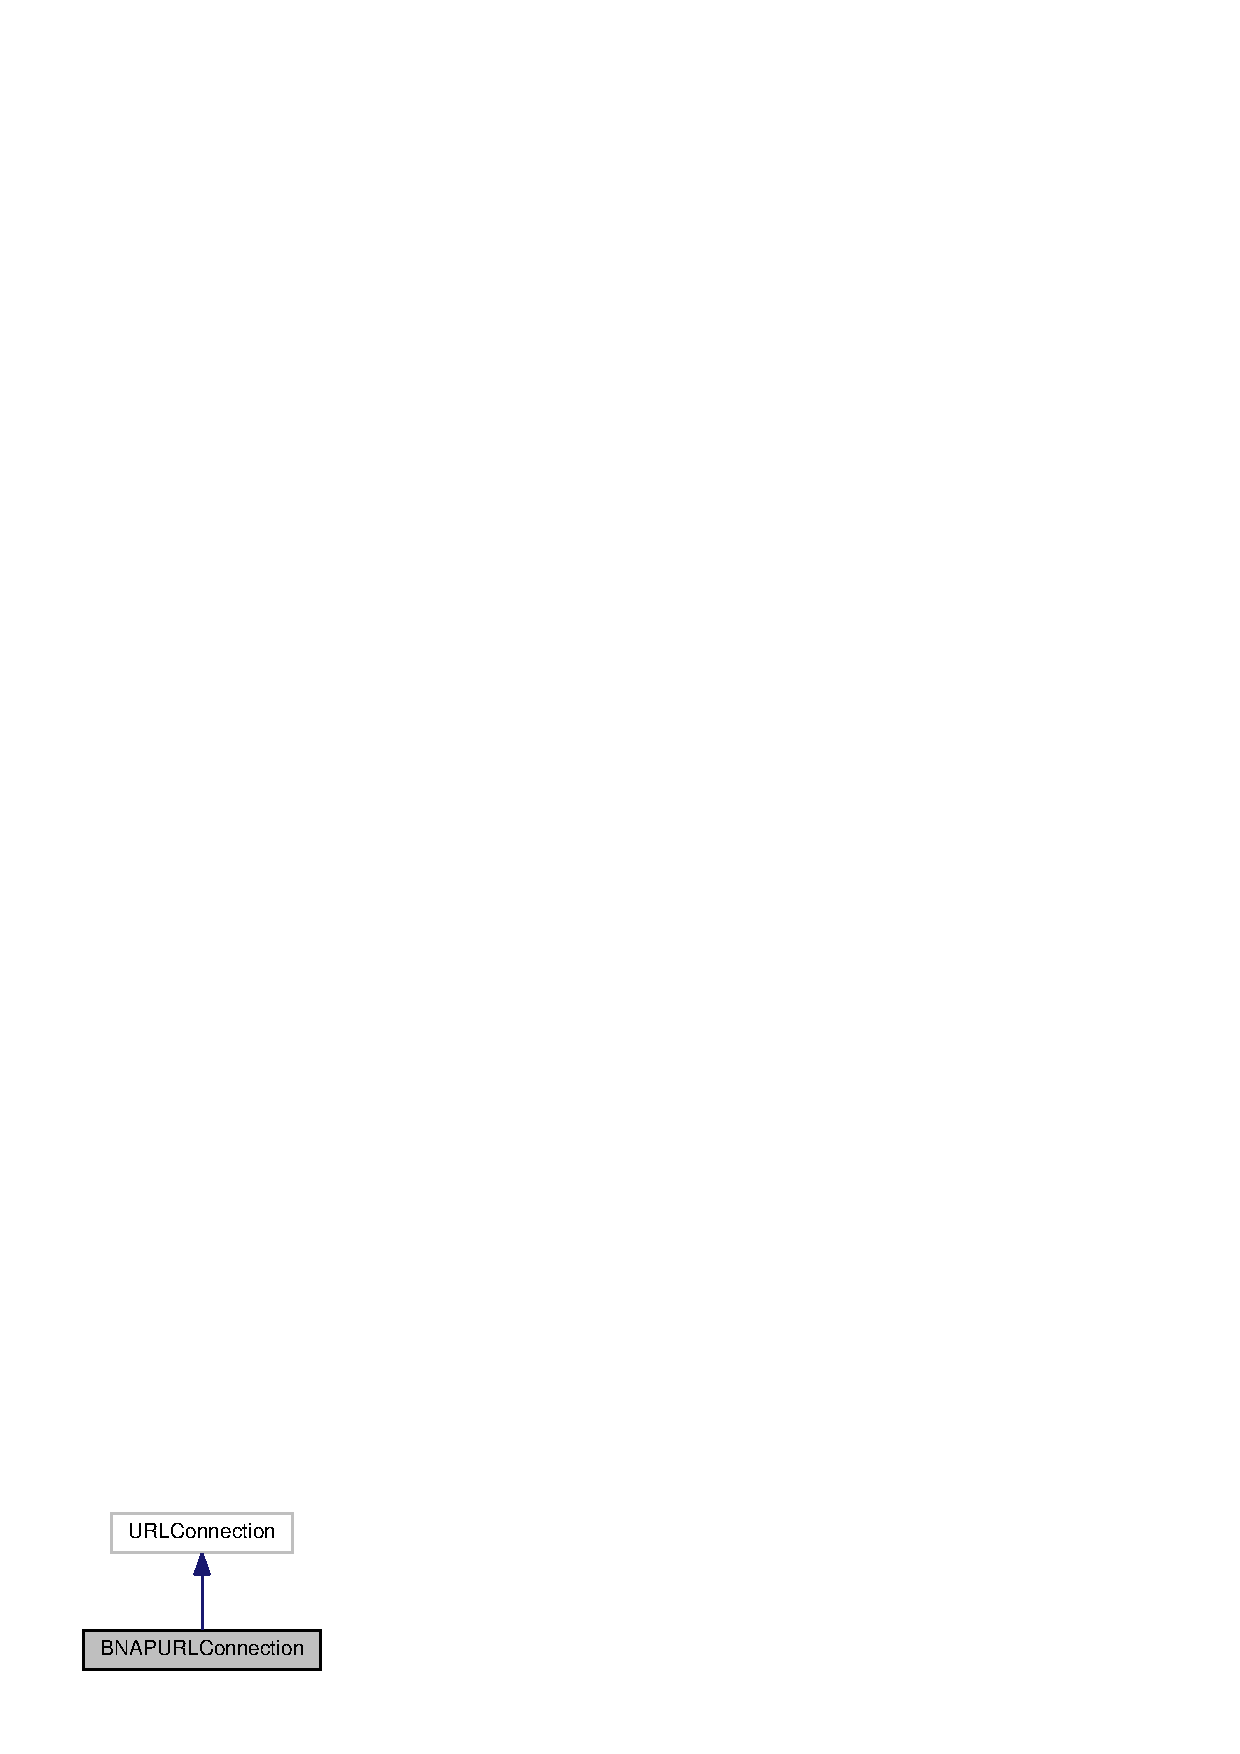
\includegraphics[width=156pt]{classorg_1_1smallfoot_1_1parser_1_1bnapsql_1_1BNAPURLConnection__inherit__graph}
\end{center}
\end{figure}


Collaboration diagram for B\+N\+A\+P\+U\+R\+L\+Connection\+:\nopagebreak
\begin{figure}[H]
\begin{center}
\leavevmode
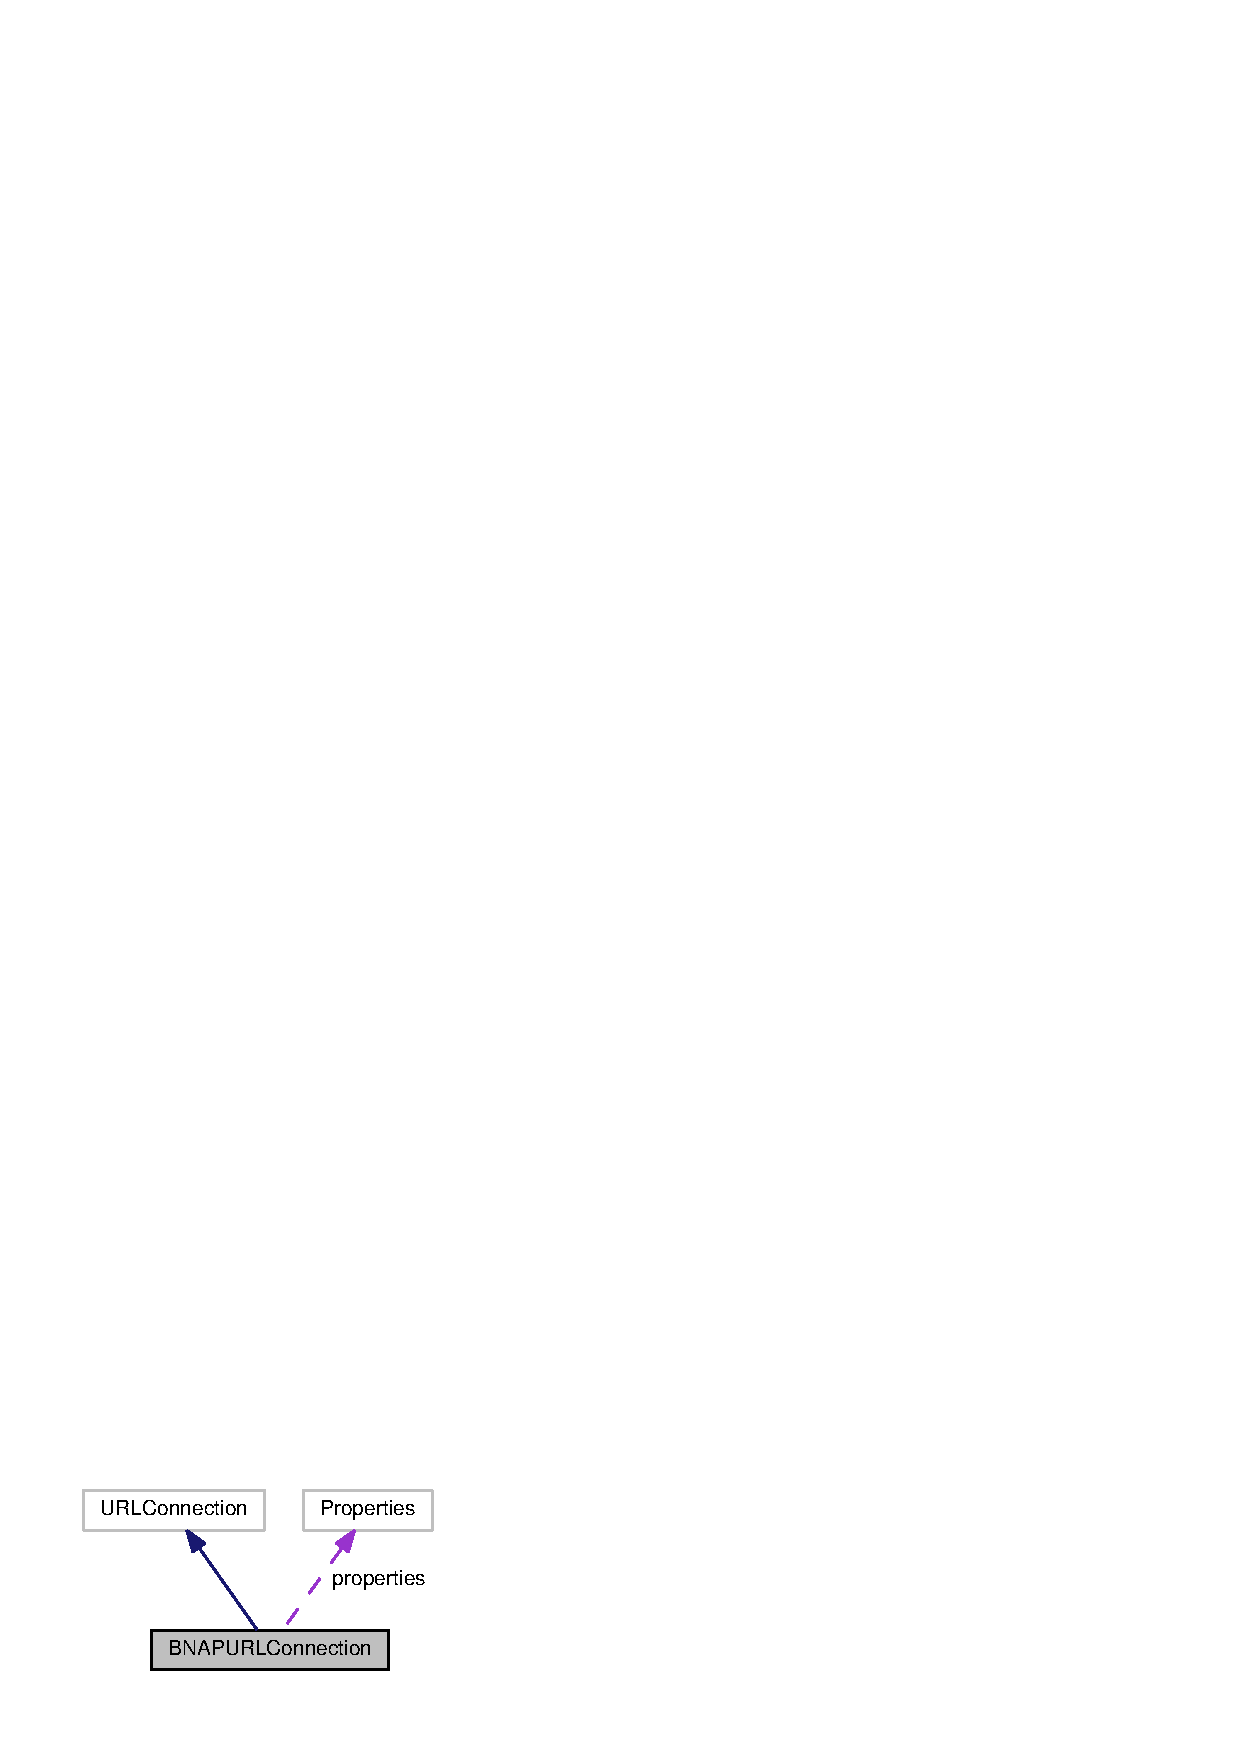
\includegraphics[width=209pt]{classorg_1_1smallfoot_1_1parser_1_1bnapsql_1_1BNAPURLConnection__coll__graph}
\end{center}
\end{figure}
\subsection*{Data Structures}
\begin{DoxyCompactItemize}
\item 
class {\bfseries Result\+C\+S\+V\+Pipe}
\begin{DoxyCompactList}\small\item\em Piped\+Output\+Stream to push out resultsets as C\+S\+V Nicknames. \end{DoxyCompactList}\item 
class {\bfseries Result\+Set\+Pipe}
\begin{DoxyCompactList}\small\item\em Piped\+Output\+Stream to push out a single column of a resultset as a stream of resulting data. \end{DoxyCompactList}\end{DoxyCompactItemize}
\subsection*{Public Member Functions}
\begin{DoxyCompactItemize}
\item 
{\bf B\+N\+A\+P\+U\+R\+L\+Connection} (String connection\+Info, String username, String password)
\item 
{\bf B\+N\+A\+P\+U\+R\+L\+Connection} (java.\+net.\+U\+R\+L url)
\begin{DoxyCompactList}\small\item\em Construct a connection U\+R\+L per {\tt http\+://www.\+postgresql.\+org/docs/9.\+3/static/libpq-\/connect.\+html\#\+L\+I\+B\+P\+Q-\/\+C\+O\+N\+N\+S\+T\+R\+I\+N\+G}. \end{DoxyCompactList}\item 
void {\bf set\+Request\+Header} (String name, String value)
\begin{DoxyCompactList}\small\item\em Stubbed, because there's no change we want to accept yet. \end{DoxyCompactList}\item 
void {\bf set\+Content\+Type} (String ignored)
\begin{DoxyCompactList}\small\item\em Stubbed, because there's no change we want to accept yet. \end{DoxyCompactList}\item 
java.\+io.\+Output\+Stream {\bf get\+Output\+Stream} ()
\begin{DoxyCompactList}\small\item\em Stubbed, because there's nothing to send us. \end{DoxyCompactList}\item 
java.\+io.\+Input\+Stream {\bf get\+Input\+Stream} ()
\item 
void {\bf connect} ()
\end{DoxyCompactItemize}
\subsection*{Protected Member Functions}
\begin{DoxyCompactItemize}
\item 
{\bf B\+N\+A\+P\+U\+R\+L\+Connection} {\bf open\+Connection} (java.\+net.\+U\+R\+L url)
\begin{DoxyCompactList}\small\item\em open\+Connection(java.\+net.\+U\+R\+L) overrides java.\+net.\+U\+R\+L\+Stream\+Handler.\+open\+Connection(\+U\+R\+L) by wrapping a pgsql client. \end{DoxyCompactList}\end{DoxyCompactItemize}


\subsection{Detailed Description}


Definition at line 36 of file B\+N\+A\+P\+U\+R\+L\+Connection.\+java.



\subsection{Constructor \& Destructor Documentation}
\index{org\+::smallfoot\+::parser\+::bnapsql\+::\+B\+N\+A\+P\+U\+R\+L\+Connection@{org\+::smallfoot\+::parser\+::bnapsql\+::\+B\+N\+A\+P\+U\+R\+L\+Connection}!B\+N\+A\+P\+U\+R\+L\+Connection@{B\+N\+A\+P\+U\+R\+L\+Connection}}
\index{B\+N\+A\+P\+U\+R\+L\+Connection@{B\+N\+A\+P\+U\+R\+L\+Connection}!org\+::smallfoot\+::parser\+::bnapsql\+::\+B\+N\+A\+P\+U\+R\+L\+Connection@{org\+::smallfoot\+::parser\+::bnapsql\+::\+B\+N\+A\+P\+U\+R\+L\+Connection}}
\subsubsection[{B\+N\+A\+P\+U\+R\+L\+Connection}]{\setlength{\rightskip}{0pt plus 5cm}{\bf B\+N\+A\+P\+U\+R\+L\+Connection} (
\begin{DoxyParamCaption}
\item[{String}]{connection\+Info, }
\item[{String}]{username, }
\item[{String}]{password}
\end{DoxyParamCaption}
)\hspace{0.3cm}{\ttfamily [inline]}}\label{classorg_1_1smallfoot_1_1parser_1_1bnapsql_1_1BNAPURLConnection_a942ebf028e78ae94fa8cc50c219ec721}


Definition at line 208 of file B\+N\+A\+P\+U\+R\+L\+Connection.\+java.

\index{org\+::smallfoot\+::parser\+::bnapsql\+::\+B\+N\+A\+P\+U\+R\+L\+Connection@{org\+::smallfoot\+::parser\+::bnapsql\+::\+B\+N\+A\+P\+U\+R\+L\+Connection}!B\+N\+A\+P\+U\+R\+L\+Connection@{B\+N\+A\+P\+U\+R\+L\+Connection}}
\index{B\+N\+A\+P\+U\+R\+L\+Connection@{B\+N\+A\+P\+U\+R\+L\+Connection}!org\+::smallfoot\+::parser\+::bnapsql\+::\+B\+N\+A\+P\+U\+R\+L\+Connection@{org\+::smallfoot\+::parser\+::bnapsql\+::\+B\+N\+A\+P\+U\+R\+L\+Connection}}
\subsubsection[{B\+N\+A\+P\+U\+R\+L\+Connection}]{\setlength{\rightskip}{0pt plus 5cm}{\bf B\+N\+A\+P\+U\+R\+L\+Connection} (
\begin{DoxyParamCaption}
\item[{java.\+net.\+U\+R\+L}]{url}
\end{DoxyParamCaption}
)\hspace{0.3cm}{\ttfamily [inline]}}\label{classorg_1_1smallfoot_1_1parser_1_1bnapsql_1_1BNAPURLConnection_a647c74134f864d18c205065944e528b1}


Construct a connection U\+R\+L per {\tt http\+://www.\+postgresql.\+org/docs/9.\+3/static/libpq-\/connect.\+html\#\+L\+I\+B\+P\+Q-\/\+C\+O\+N\+N\+S\+T\+R\+I\+N\+G}. 


\begin{DoxyParams}{Parameters}
{\em url} & connection url of the form \char`\"{}$<$proto$>$\+://user\+:pass@host\+:port/database\char`\"{} parsed by a Java.\+net.\+U\+R\+L constructor. \\
\hline
\end{DoxyParams}


Definition at line 222 of file B\+N\+A\+P\+U\+R\+L\+Connection.\+java.



\subsection{Member Function Documentation}
\index{org\+::smallfoot\+::parser\+::bnapsql\+::\+B\+N\+A\+P\+U\+R\+L\+Connection@{org\+::smallfoot\+::parser\+::bnapsql\+::\+B\+N\+A\+P\+U\+R\+L\+Connection}!connect@{connect}}
\index{connect@{connect}!org\+::smallfoot\+::parser\+::bnapsql\+::\+B\+N\+A\+P\+U\+R\+L\+Connection@{org\+::smallfoot\+::parser\+::bnapsql\+::\+B\+N\+A\+P\+U\+R\+L\+Connection}}
\subsubsection[{connect}]{\setlength{\rightskip}{0pt plus 5cm}void connect (
\begin{DoxyParamCaption}
{}
\end{DoxyParamCaption}
)\hspace{0.3cm}{\ttfamily [inline]}}\label{classorg_1_1smallfoot_1_1parser_1_1bnapsql_1_1BNAPURLConnection_a1396bf9b5defe9fa844a63b5cd40ac0e}


Definition at line 367 of file B\+N\+A\+P\+U\+R\+L\+Connection.\+java.



Referenced by B\+N\+A\+P\+U\+R\+L\+Connection.\+get\+Input\+Stream().

\index{org\+::smallfoot\+::parser\+::bnapsql\+::\+B\+N\+A\+P\+U\+R\+L\+Connection@{org\+::smallfoot\+::parser\+::bnapsql\+::\+B\+N\+A\+P\+U\+R\+L\+Connection}!get\+Input\+Stream@{get\+Input\+Stream}}
\index{get\+Input\+Stream@{get\+Input\+Stream}!org\+::smallfoot\+::parser\+::bnapsql\+::\+B\+N\+A\+P\+U\+R\+L\+Connection@{org\+::smallfoot\+::parser\+::bnapsql\+::\+B\+N\+A\+P\+U\+R\+L\+Connection}}
\subsubsection[{get\+Input\+Stream}]{\setlength{\rightskip}{0pt plus 5cm}java.\+io.\+Input\+Stream get\+Input\+Stream (
\begin{DoxyParamCaption}
{}
\end{DoxyParamCaption}
)\hspace{0.3cm}{\ttfamily [inline]}}\label{classorg_1_1smallfoot_1_1parser_1_1bnapsql_1_1BNAPURLConnection_a0924d1107a459be632532ef34324494e}
\begin{DoxyRefDesc}{J\+V\+M Options}
\item[{\bf J\+V\+M Options}]{\bfseries debug.\+carleton}\+: For testing and additional info, -\/\+Ddebug.\+carleton causes the \char`\"{}old\char`\"{} query to be swapped with a pull from hba\+\_\+target\+\_\+info \end{DoxyRefDesc}


Definition at line 295 of file B\+N\+A\+P\+U\+R\+L\+Connection.\+java.



References B\+N\+A\+P\+U\+R\+L\+Connection.\+connect().



Here is the call graph for this function\+:\nopagebreak
\begin{figure}[H]
\begin{center}
\leavevmode
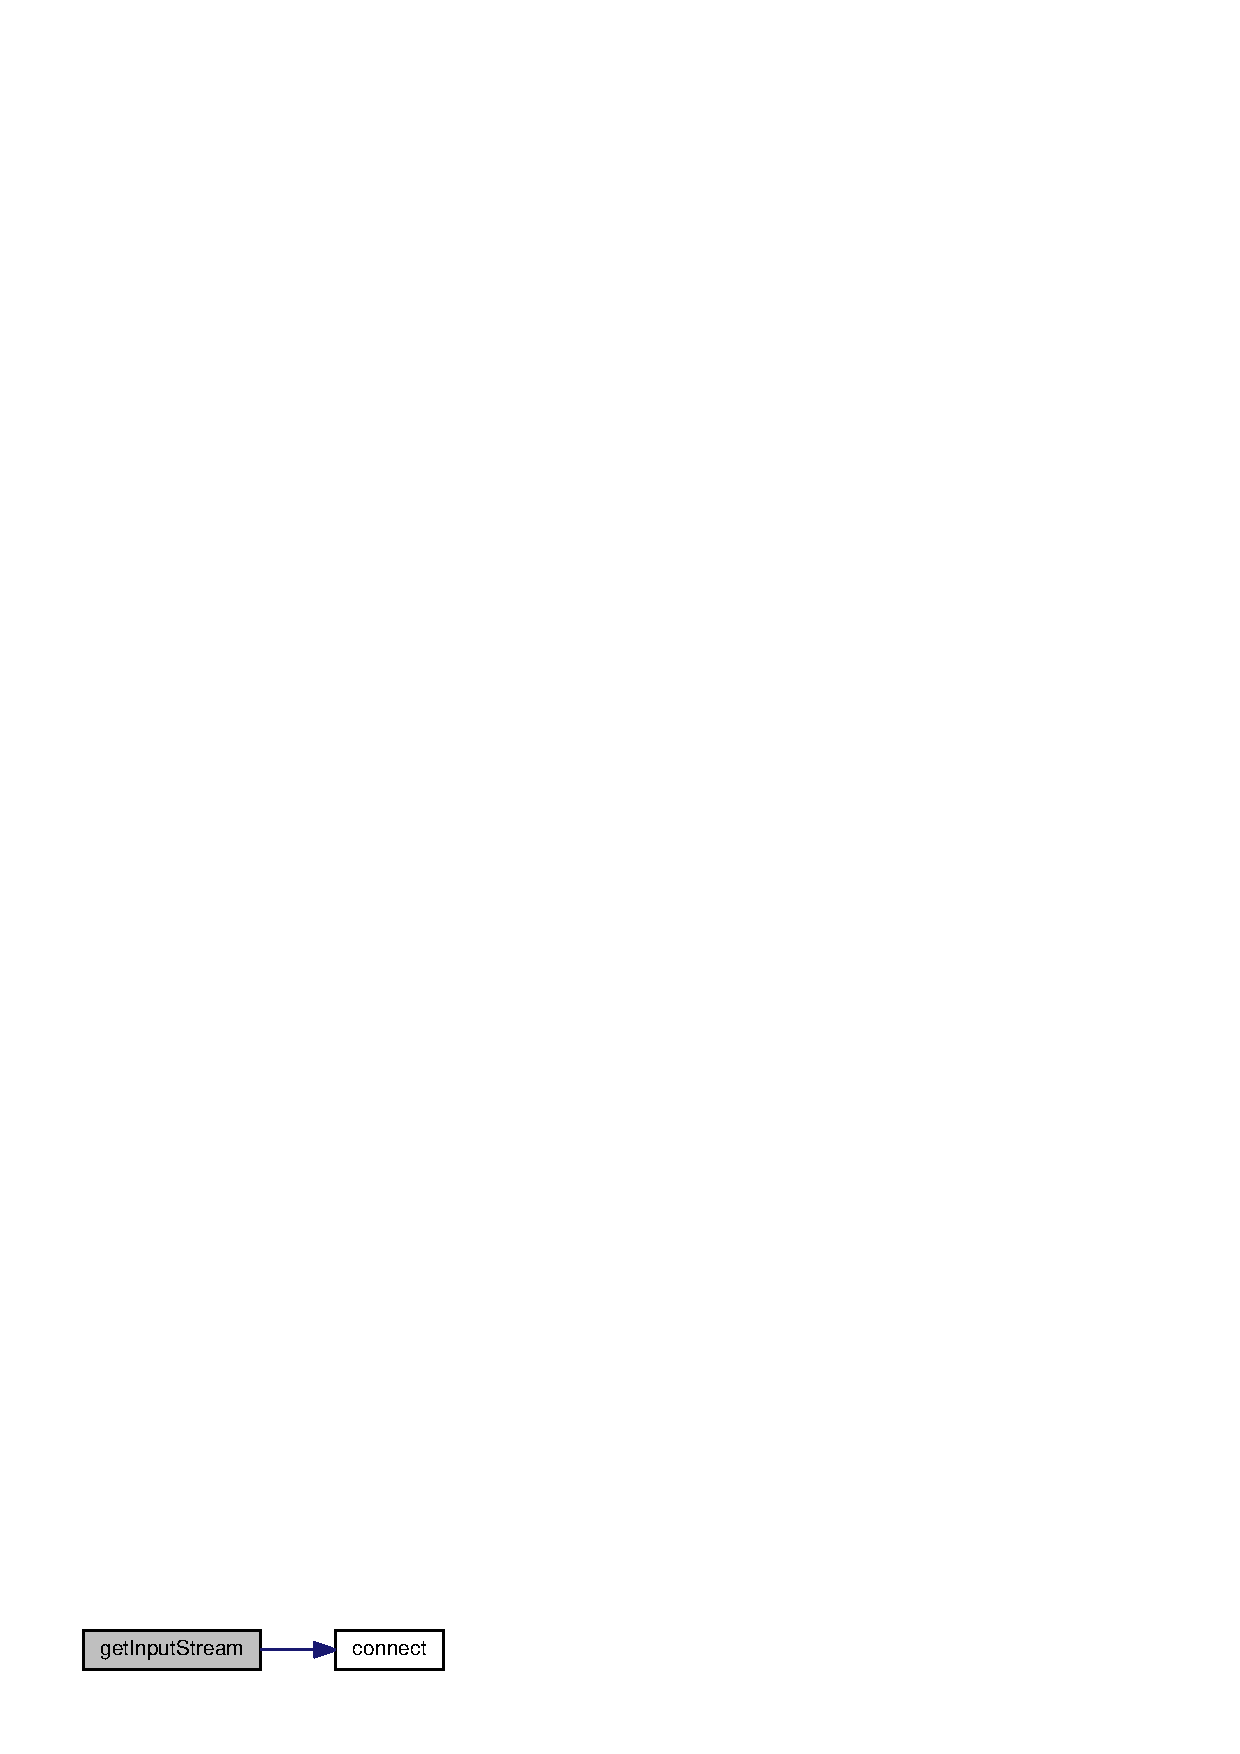
\includegraphics[width=216pt]{classorg_1_1smallfoot_1_1parser_1_1bnapsql_1_1BNAPURLConnection_a0924d1107a459be632532ef34324494e_cgraph}
\end{center}
\end{figure}


\index{org\+::smallfoot\+::parser\+::bnapsql\+::\+B\+N\+A\+P\+U\+R\+L\+Connection@{org\+::smallfoot\+::parser\+::bnapsql\+::\+B\+N\+A\+P\+U\+R\+L\+Connection}!get\+Output\+Stream@{get\+Output\+Stream}}
\index{get\+Output\+Stream@{get\+Output\+Stream}!org\+::smallfoot\+::parser\+::bnapsql\+::\+B\+N\+A\+P\+U\+R\+L\+Connection@{org\+::smallfoot\+::parser\+::bnapsql\+::\+B\+N\+A\+P\+U\+R\+L\+Connection}}
\subsubsection[{get\+Output\+Stream}]{\setlength{\rightskip}{0pt plus 5cm}java.\+io.\+Output\+Stream get\+Output\+Stream (
\begin{DoxyParamCaption}
{}
\end{DoxyParamCaption}
)\hspace{0.3cm}{\ttfamily [inline]}}\label{classorg_1_1smallfoot_1_1parser_1_1bnapsql_1_1BNAPURLConnection_a4170f42681efaf92df5c2030f5298905}


Stubbed, because there's nothing to send us. 

Oh how did I get caught in the \char`\"{}\+Royal '\+We'\char`\"{} ? 

Definition at line 280 of file B\+N\+A\+P\+U\+R\+L\+Connection.\+java.

\index{org\+::smallfoot\+::parser\+::bnapsql\+::\+B\+N\+A\+P\+U\+R\+L\+Connection@{org\+::smallfoot\+::parser\+::bnapsql\+::\+B\+N\+A\+P\+U\+R\+L\+Connection}!open\+Connection@{open\+Connection}}
\index{open\+Connection@{open\+Connection}!org\+::smallfoot\+::parser\+::bnapsql\+::\+B\+N\+A\+P\+U\+R\+L\+Connection@{org\+::smallfoot\+::parser\+::bnapsql\+::\+B\+N\+A\+P\+U\+R\+L\+Connection}}
\subsubsection[{open\+Connection}]{\setlength{\rightskip}{0pt plus 5cm}{\bf B\+N\+A\+P\+U\+R\+L\+Connection} open\+Connection (
\begin{DoxyParamCaption}
\item[{java.\+net.\+U\+R\+L}]{url}
\end{DoxyParamCaption}
)\hspace{0.3cm}{\ttfamily [inline]}, {\ttfamily [protected]}}\label{classorg_1_1smallfoot_1_1parser_1_1bnapsql_1_1BNAPURLConnection_a4ad7fe915d0e811bd8f8ac7b5d22f4f9}


open\+Connection(java.\+net.\+U\+R\+L) overrides java.\+net.\+U\+R\+L\+Stream\+Handler.\+open\+Connection(\+U\+R\+L) by wrapping a pgsql client. 

\begin{DoxyReturn}{Returns}
populated connection as org.\+smallfoot.\+bnapsql.\+B\+N\+A\+P\+U\+R\+L\+Connection(\+Connection) 
\end{DoxyReturn}

\begin{DoxyParams}{Parameters}
{\em url} & U\+R\+L to connect to \\
\hline
\end{DoxyParams}


Definition at line 346 of file B\+N\+A\+P\+U\+R\+L\+Connection.\+java.

\index{org\+::smallfoot\+::parser\+::bnapsql\+::\+B\+N\+A\+P\+U\+R\+L\+Connection@{org\+::smallfoot\+::parser\+::bnapsql\+::\+B\+N\+A\+P\+U\+R\+L\+Connection}!set\+Content\+Type@{set\+Content\+Type}}
\index{set\+Content\+Type@{set\+Content\+Type}!org\+::smallfoot\+::parser\+::bnapsql\+::\+B\+N\+A\+P\+U\+R\+L\+Connection@{org\+::smallfoot\+::parser\+::bnapsql\+::\+B\+N\+A\+P\+U\+R\+L\+Connection}}
\subsubsection[{set\+Content\+Type}]{\setlength{\rightskip}{0pt plus 5cm}void set\+Content\+Type (
\begin{DoxyParamCaption}
\item[{String}]{ignored}
\end{DoxyParamCaption}
)\hspace{0.3cm}{\ttfamily [inline]}}\label{classorg_1_1smallfoot_1_1parser_1_1bnapsql_1_1BNAPURLConnection_aa608e58be69b0389d82d846a25091d36}


Stubbed, because there's no change we want to accept yet. 

Sorry, apparently \char`\"{}at this time\char`\"{} is more professional, if you listen to the wordy airport announcements.


\begin{DoxyParams}{Parameters}
{\em ignored} & ignored \\
\hline
\end{DoxyParams}


Definition at line 275 of file B\+N\+A\+P\+U\+R\+L\+Connection.\+java.

\index{org\+::smallfoot\+::parser\+::bnapsql\+::\+B\+N\+A\+P\+U\+R\+L\+Connection@{org\+::smallfoot\+::parser\+::bnapsql\+::\+B\+N\+A\+P\+U\+R\+L\+Connection}!set\+Request\+Header@{set\+Request\+Header}}
\index{set\+Request\+Header@{set\+Request\+Header}!org\+::smallfoot\+::parser\+::bnapsql\+::\+B\+N\+A\+P\+U\+R\+L\+Connection@{org\+::smallfoot\+::parser\+::bnapsql\+::\+B\+N\+A\+P\+U\+R\+L\+Connection}}
\subsubsection[{set\+Request\+Header}]{\setlength{\rightskip}{0pt plus 5cm}void set\+Request\+Header (
\begin{DoxyParamCaption}
\item[{String}]{name, }
\item[{String}]{value}
\end{DoxyParamCaption}
)\hspace{0.3cm}{\ttfamily [inline]}}\label{classorg_1_1smallfoot_1_1parser_1_1bnapsql_1_1BNAPURLConnection_ac2f45f32dfcaef408189cabb2644841c}


Stubbed, because there's no change we want to accept yet. 

Sorry, apparently \char`\"{}at this time\char`\"{} is more professional, if you listen to the wordy airport announcements.


\begin{DoxyParams}{Parameters}
{\em name} & ignored \\
\hline
{\em value} & ignored \\
\hline
\end{DoxyParams}


Definition at line 268 of file B\+N\+A\+P\+U\+R\+L\+Connection.\+java.



The documentation for this class was generated from the following file\+:\begin{DoxyCompactItemize}
\item 
java/{\bf B\+N\+A\+P\+U\+R\+L\+Connection.\+java}\end{DoxyCompactItemize}

\section{B\+N\+A\+Zone\+Parser Class Reference}
\label{classorg_1_1smallfoot_1_1parser_1_1zone_1_1BNAZoneParser}\index{B\+N\+A\+Zone\+Parser@{B\+N\+A\+Zone\+Parser}}


Inheritance diagram for B\+N\+A\+Zone\+Parser\+:\nopagebreak
\begin{figure}[H]
\begin{center}
\leavevmode
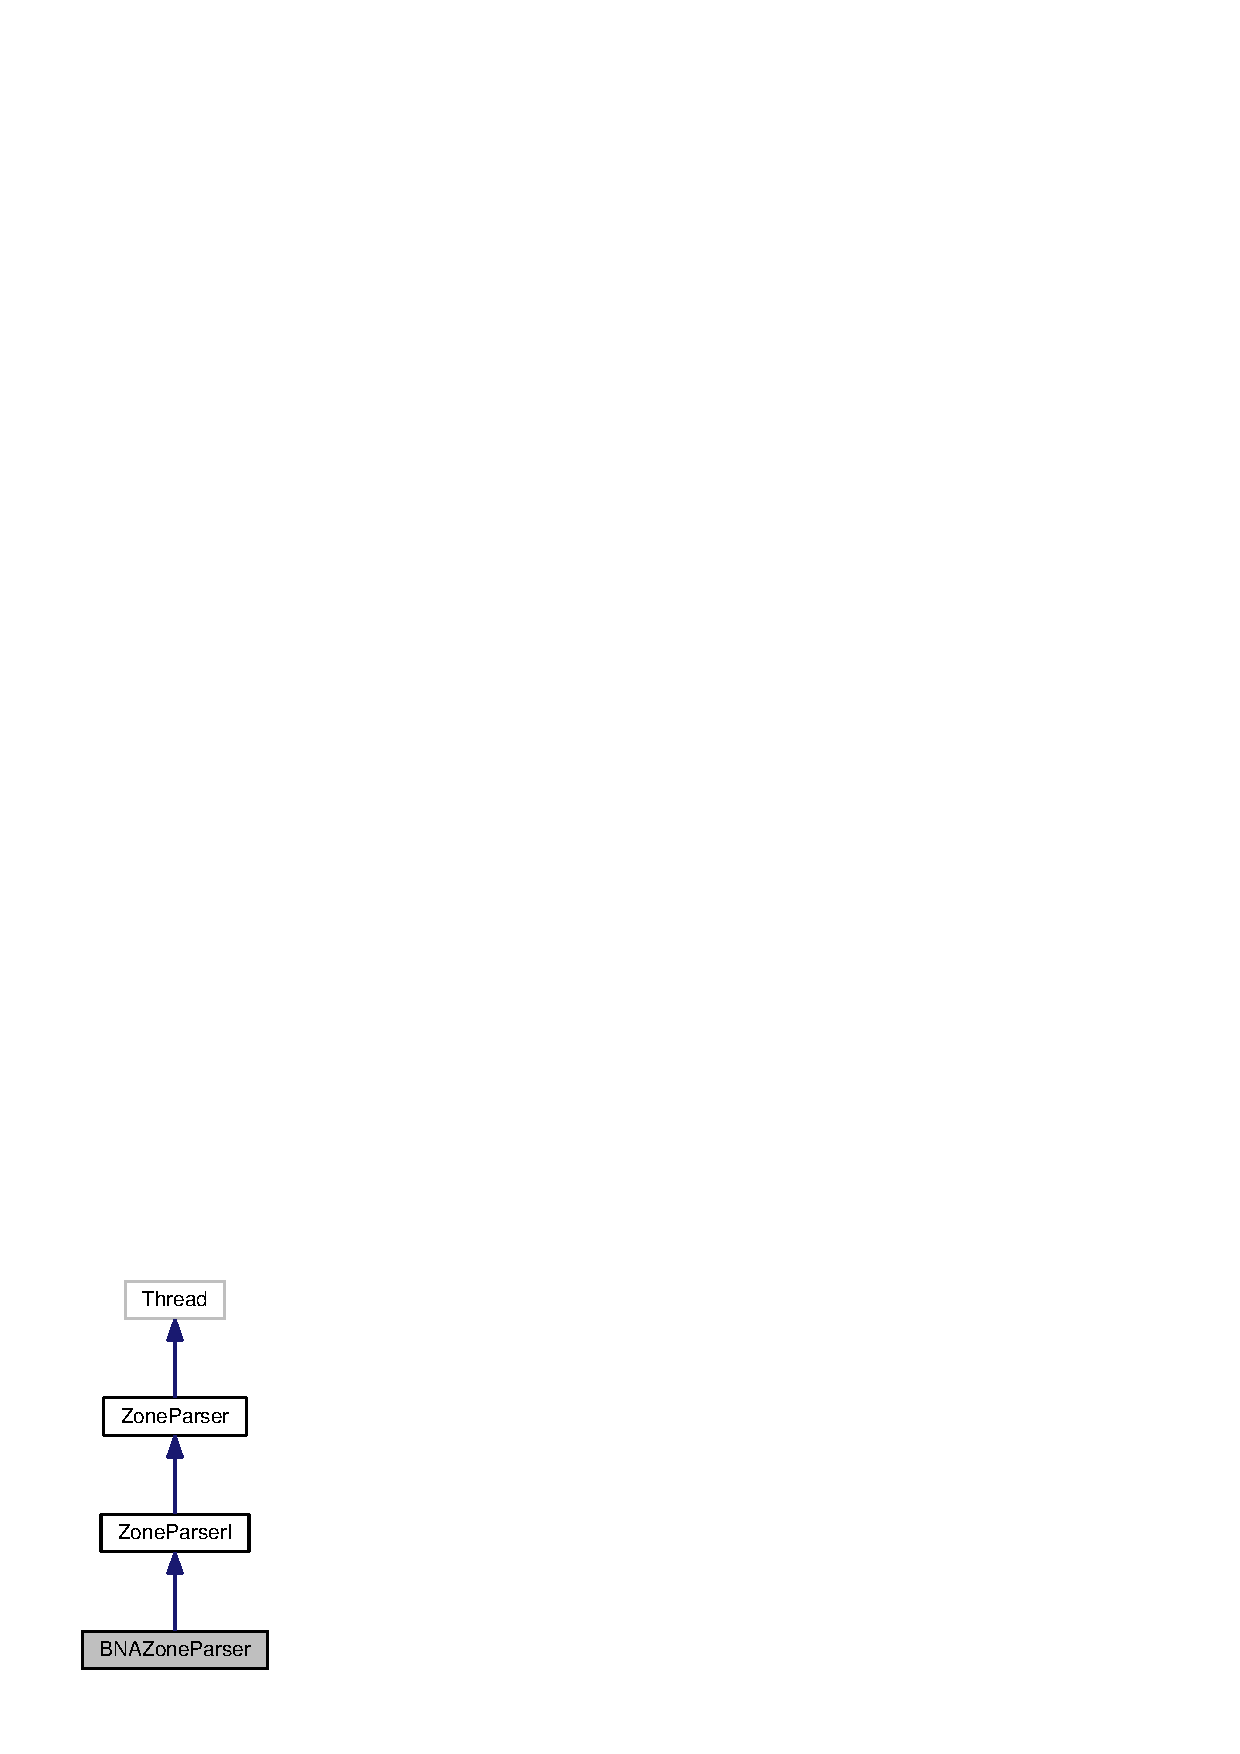
\includegraphics[width=132pt]{classorg_1_1smallfoot_1_1parser_1_1zone_1_1BNAZoneParser__inherit__graph}
\end{center}
\end{figure}


Collaboration diagram for B\+N\+A\+Zone\+Parser\+:
\nopagebreak
\begin{figure}[H]
\begin{center}
\leavevmode
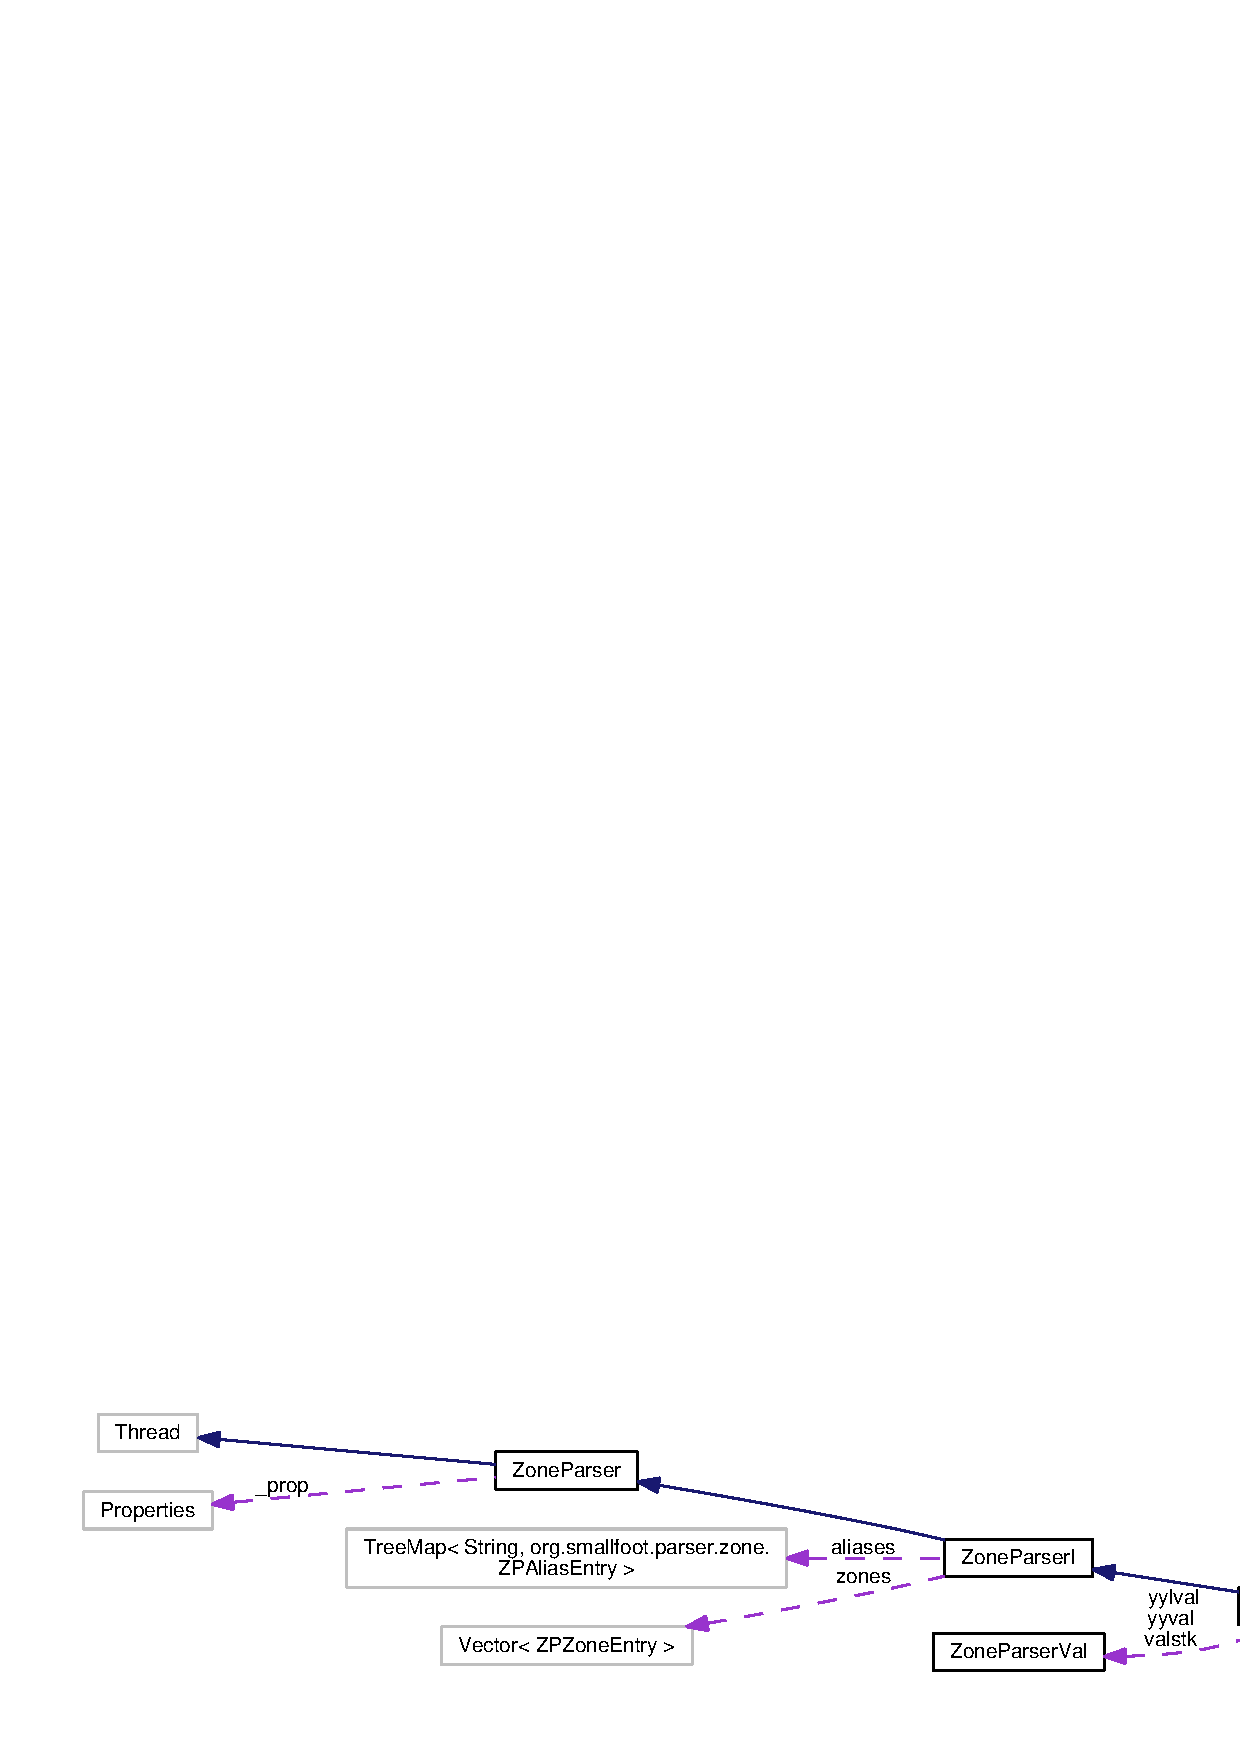
\includegraphics[width=350pt]{classorg_1_1smallfoot_1_1parser_1_1zone_1_1BNAZoneParser__coll__graph}
\end{center}
\end{figure}
\subsection*{Public Member Functions}
\begin{DoxyCompactItemize}
\item 
void {\bf parse} ()
\item 
void {\bf set\+Reader} (Reader in)
\item 
void {\bf run} ()
\item 
void {\bf set\+Debug} (boolean debug)
\item 
{\bf B\+N\+A\+Zone\+Parser} (Input\+Stream in, boolean debug\+Me)
\item 
{\bf B\+N\+A\+Zone\+Parser} (Input\+Stream in)
\item 
{\bf B\+N\+A\+Zone\+Parser} (java.\+util.\+Properties in)
\end{DoxyCompactItemize}
\subsection*{Static Public Member Functions}
\begin{DoxyCompactItemize}
\item 
static void {\bf main} (String args[$\,$])
\end{DoxyCompactItemize}
\subsection*{Static Public Attributes}
\begin{DoxyCompactItemize}
\item 
static final short {\bf T\+O\+K01} =1
\item 
static final short {\bf T\+O\+K02} =2
\item 
static final short {\bf T\+O\+K03} =3
\item 
static final short {\bf T\+O\+K05} =5
\item 
static final short {\bf T\+O\+K07} =7
\item 
static final short {\bf A\+L\+P\+H\+A\+N\+U\+M} =257
\item 
static final short {\bf Y\+Y\+E\+R\+R\+C\+O\+D\+E} =256
\end{DoxyCompactItemize}


\subsection{Detailed Description}


Definition at line 50 of file B\+N\+A\+Zone\+Parser.\+java.



\subsection{Constructor \& Destructor Documentation}
\index{org\+::smallfoot\+::parser\+::zone\+::\+B\+N\+A\+Zone\+Parser@{org\+::smallfoot\+::parser\+::zone\+::\+B\+N\+A\+Zone\+Parser}!B\+N\+A\+Zone\+Parser@{B\+N\+A\+Zone\+Parser}}
\index{B\+N\+A\+Zone\+Parser@{B\+N\+A\+Zone\+Parser}!org\+::smallfoot\+::parser\+::zone\+::\+B\+N\+A\+Zone\+Parser@{org\+::smallfoot\+::parser\+::zone\+::\+B\+N\+A\+Zone\+Parser}}
\subsubsection[{B\+N\+A\+Zone\+Parser}]{\setlength{\rightskip}{0pt plus 5cm}{\bf B\+N\+A\+Zone\+Parser} (
\begin{DoxyParamCaption}
\item[{Input\+Stream}]{in, }
\item[{boolean}]{debug\+Me}
\end{DoxyParamCaption}
)\hspace{0.3cm}{\ttfamily [inline]}}\label{classorg_1_1smallfoot_1_1parser_1_1zone_1_1BNAZoneParser_a461606a38dc40cb68f480cab9878d620}


Definition at line 445 of file B\+N\+A\+Zone\+Parser.\+java.



Referenced by B\+N\+A\+Zone\+Parser.\+main().

\index{org\+::smallfoot\+::parser\+::zone\+::\+B\+N\+A\+Zone\+Parser@{org\+::smallfoot\+::parser\+::zone\+::\+B\+N\+A\+Zone\+Parser}!B\+N\+A\+Zone\+Parser@{B\+N\+A\+Zone\+Parser}}
\index{B\+N\+A\+Zone\+Parser@{B\+N\+A\+Zone\+Parser}!org\+::smallfoot\+::parser\+::zone\+::\+B\+N\+A\+Zone\+Parser@{org\+::smallfoot\+::parser\+::zone\+::\+B\+N\+A\+Zone\+Parser}}
\subsubsection[{B\+N\+A\+Zone\+Parser}]{\setlength{\rightskip}{0pt plus 5cm}{\bf B\+N\+A\+Zone\+Parser} (
\begin{DoxyParamCaption}
\item[{Input\+Stream}]{in}
\end{DoxyParamCaption}
)\hspace{0.3cm}{\ttfamily [inline]}}\label{classorg_1_1smallfoot_1_1parser_1_1zone_1_1BNAZoneParser_a0908383bf408f9defeb19ebcd0d22a41}


Definition at line 446 of file B\+N\+A\+Zone\+Parser.\+java.

\index{org\+::smallfoot\+::parser\+::zone\+::\+B\+N\+A\+Zone\+Parser@{org\+::smallfoot\+::parser\+::zone\+::\+B\+N\+A\+Zone\+Parser}!B\+N\+A\+Zone\+Parser@{B\+N\+A\+Zone\+Parser}}
\index{B\+N\+A\+Zone\+Parser@{B\+N\+A\+Zone\+Parser}!org\+::smallfoot\+::parser\+::zone\+::\+B\+N\+A\+Zone\+Parser@{org\+::smallfoot\+::parser\+::zone\+::\+B\+N\+A\+Zone\+Parser}}
\subsubsection[{B\+N\+A\+Zone\+Parser}]{\setlength{\rightskip}{0pt plus 5cm}{\bf B\+N\+A\+Zone\+Parser} (
\begin{DoxyParamCaption}
\item[{java.\+util.\+Properties}]{in}
\end{DoxyParamCaption}
)\hspace{0.3cm}{\ttfamily [inline]}}\label{classorg_1_1smallfoot_1_1parser_1_1zone_1_1BNAZoneParser_a7f848f7fa16da15b846b783d07328f76}


Definition at line 447 of file B\+N\+A\+Zone\+Parser.\+java.



\subsection{Member Function Documentation}
\index{org\+::smallfoot\+::parser\+::zone\+::\+B\+N\+A\+Zone\+Parser@{org\+::smallfoot\+::parser\+::zone\+::\+B\+N\+A\+Zone\+Parser}!main@{main}}
\index{main@{main}!org\+::smallfoot\+::parser\+::zone\+::\+B\+N\+A\+Zone\+Parser@{org\+::smallfoot\+::parser\+::zone\+::\+B\+N\+A\+Zone\+Parser}}
\subsubsection[{main}]{\setlength{\rightskip}{0pt plus 5cm}static void main (
\begin{DoxyParamCaption}
\item[{String}]{args[$\,$]}
\end{DoxyParamCaption}
)\hspace{0.3cm}{\ttfamily [inline]}, {\ttfamily [static]}}\label{classorg_1_1smallfoot_1_1parser_1_1zone_1_1BNAZoneParser_a75988cf84fc6ee7a2ebff36e363021aa}


Definition at line 450 of file B\+N\+A\+Zone\+Parser.\+java.



References B\+N\+A\+Zone\+Parser.\+B\+N\+A\+Zone\+Parser(), and Zone\+Parser\+I.\+test\+Summary().



Here is the call graph for this function\+:\nopagebreak
\begin{figure}[H]
\begin{center}
\leavevmode
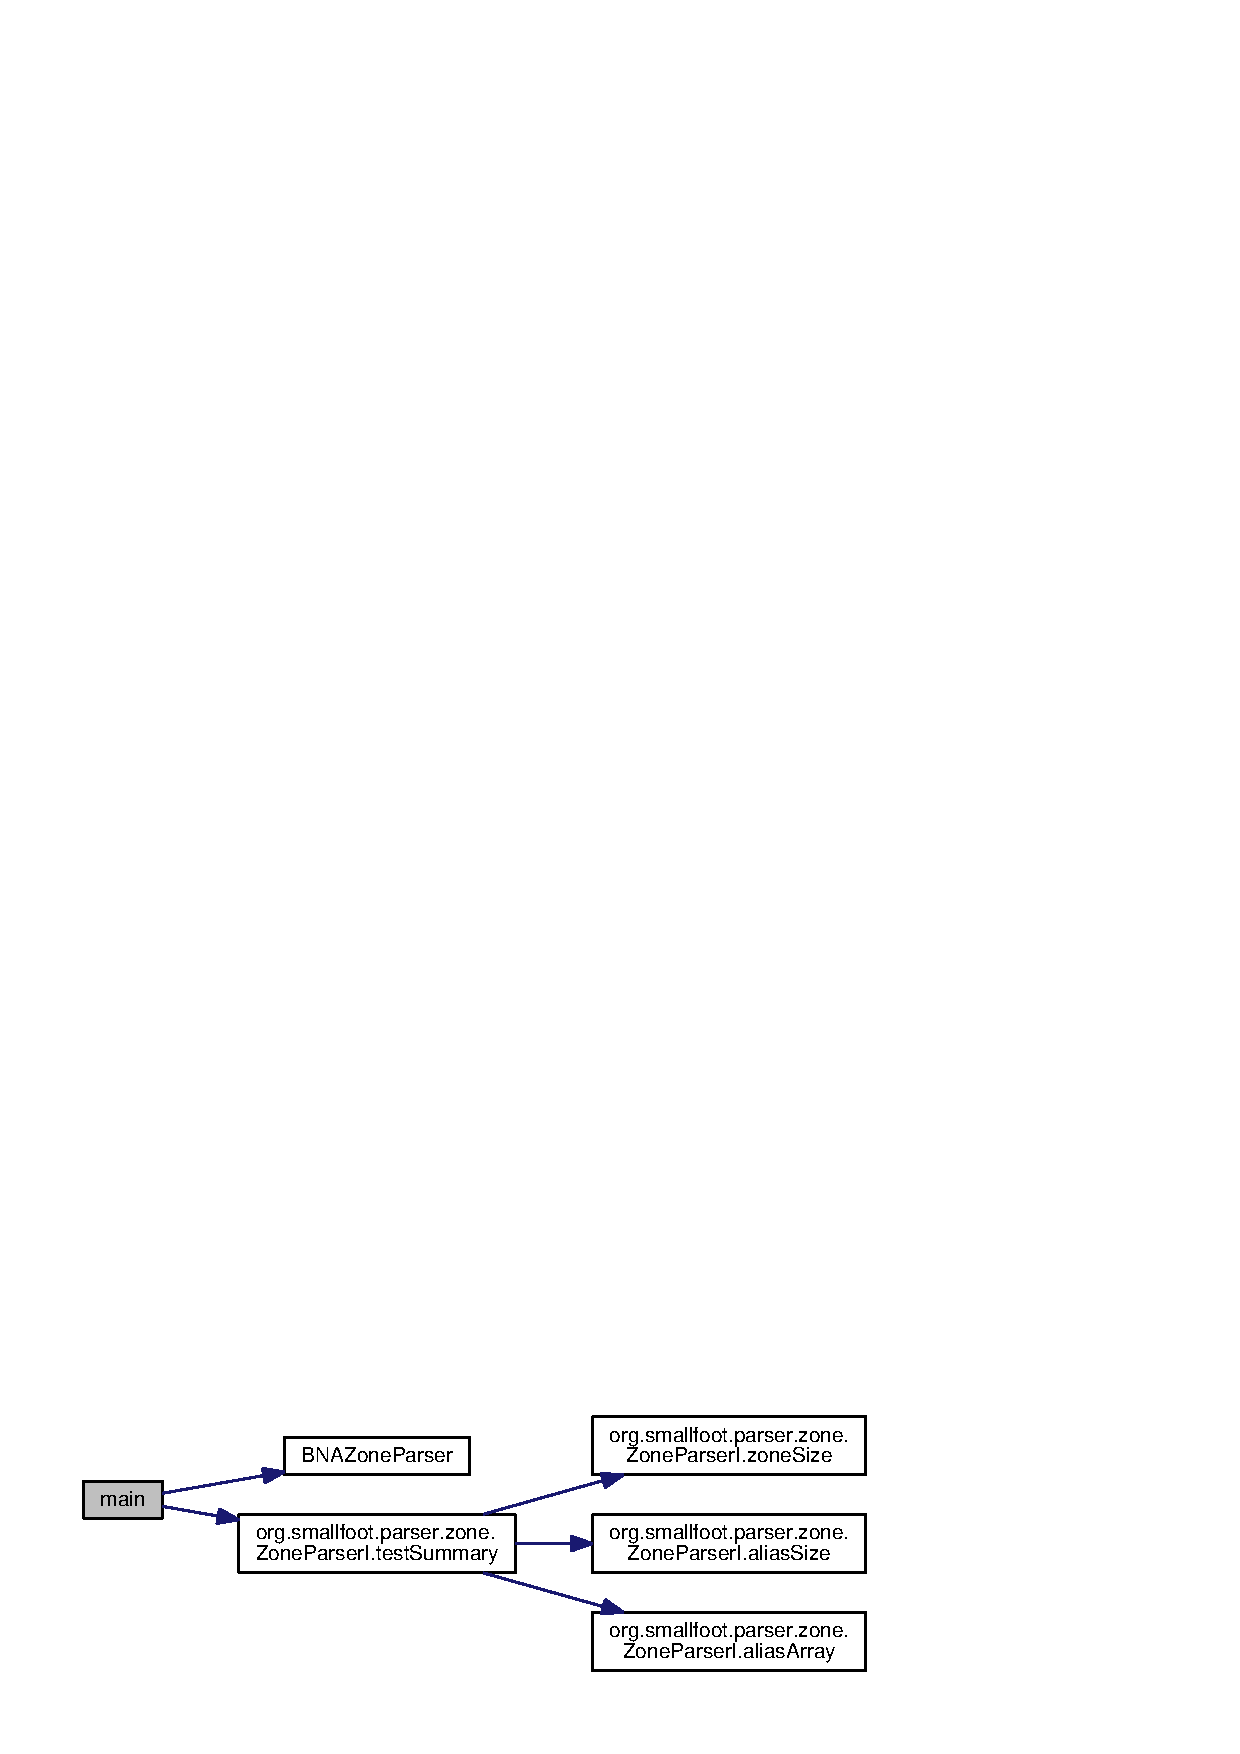
\includegraphics[width=350pt]{classorg_1_1smallfoot_1_1parser_1_1zone_1_1BNAZoneParser_a75988cf84fc6ee7a2ebff36e363021aa_cgraph}
\end{center}
\end{figure}


\index{org\+::smallfoot\+::parser\+::zone\+::\+B\+N\+A\+Zone\+Parser@{org\+::smallfoot\+::parser\+::zone\+::\+B\+N\+A\+Zone\+Parser}!parse@{parse}}
\index{parse@{parse}!org\+::smallfoot\+::parser\+::zone\+::\+B\+N\+A\+Zone\+Parser@{org\+::smallfoot\+::parser\+::zone\+::\+B\+N\+A\+Zone\+Parser}}
\subsubsection[{parse}]{\setlength{\rightskip}{0pt plus 5cm}void parse (
\begin{DoxyParamCaption}
{}
\end{DoxyParamCaption}
)\hspace{0.3cm}{\ttfamily [inline]}}\label{classorg_1_1smallfoot_1_1parser_1_1zone_1_1BNAZoneParser_ad7c704b34912678d95c13243cacf9d7f}


Definition at line 392 of file B\+N\+A\+Zone\+Parser.\+java.

\index{org\+::smallfoot\+::parser\+::zone\+::\+B\+N\+A\+Zone\+Parser@{org\+::smallfoot\+::parser\+::zone\+::\+B\+N\+A\+Zone\+Parser}!run@{run}}
\index{run@{run}!org\+::smallfoot\+::parser\+::zone\+::\+B\+N\+A\+Zone\+Parser@{org\+::smallfoot\+::parser\+::zone\+::\+B\+N\+A\+Zone\+Parser}}
\subsubsection[{run}]{\setlength{\rightskip}{0pt plus 5cm}void run (
\begin{DoxyParamCaption}
{}
\end{DoxyParamCaption}
)\hspace{0.3cm}{\ttfamily [inline]}}\label{classorg_1_1smallfoot_1_1parser_1_1zone_1_1BNAZoneParser_a13a43e6d814de94978c515cb084873b1}


Definition at line 432 of file B\+N\+A\+Zone\+Parser.\+java.

\index{org\+::smallfoot\+::parser\+::zone\+::\+B\+N\+A\+Zone\+Parser@{org\+::smallfoot\+::parser\+::zone\+::\+B\+N\+A\+Zone\+Parser}!set\+Debug@{set\+Debug}}
\index{set\+Debug@{set\+Debug}!org\+::smallfoot\+::parser\+::zone\+::\+B\+N\+A\+Zone\+Parser@{org\+::smallfoot\+::parser\+::zone\+::\+B\+N\+A\+Zone\+Parser}}
\subsubsection[{set\+Debug}]{\setlength{\rightskip}{0pt plus 5cm}void set\+Debug (
\begin{DoxyParamCaption}
\item[{boolean}]{debug}
\end{DoxyParamCaption}
)\hspace{0.3cm}{\ttfamily [inline]}}\label{classorg_1_1smallfoot_1_1parser_1_1zone_1_1BNAZoneParser_a6c13d260cf71d0554f789c4641a9f18b}


Definition at line 444 of file B\+N\+A\+Zone\+Parser.\+java.

\index{org\+::smallfoot\+::parser\+::zone\+::\+B\+N\+A\+Zone\+Parser@{org\+::smallfoot\+::parser\+::zone\+::\+B\+N\+A\+Zone\+Parser}!set\+Reader@{set\+Reader}}
\index{set\+Reader@{set\+Reader}!org\+::smallfoot\+::parser\+::zone\+::\+B\+N\+A\+Zone\+Parser@{org\+::smallfoot\+::parser\+::zone\+::\+B\+N\+A\+Zone\+Parser}}
\subsubsection[{set\+Reader}]{\setlength{\rightskip}{0pt plus 5cm}void set\+Reader (
\begin{DoxyParamCaption}
\item[{Reader}]{in}
\end{DoxyParamCaption}
)\hspace{0.3cm}{\ttfamily [inline]}}\label{classorg_1_1smallfoot_1_1parser_1_1zone_1_1BNAZoneParser_a5deab139f9ad4072e1a497c5cccda0ea}


Definition at line 404 of file B\+N\+A\+Zone\+Parser.\+java.



\subsection{Field Documentation}
\index{org\+::smallfoot\+::parser\+::zone\+::\+B\+N\+A\+Zone\+Parser@{org\+::smallfoot\+::parser\+::zone\+::\+B\+N\+A\+Zone\+Parser}!A\+L\+P\+H\+A\+N\+U\+M@{A\+L\+P\+H\+A\+N\+U\+M}}
\index{A\+L\+P\+H\+A\+N\+U\+M@{A\+L\+P\+H\+A\+N\+U\+M}!org\+::smallfoot\+::parser\+::zone\+::\+B\+N\+A\+Zone\+Parser@{org\+::smallfoot\+::parser\+::zone\+::\+B\+N\+A\+Zone\+Parser}}
\subsubsection[{A\+L\+P\+H\+A\+N\+U\+M}]{\setlength{\rightskip}{0pt plus 5cm}final short A\+L\+P\+H\+A\+N\+U\+M =257\hspace{0.3cm}{\ttfamily [static]}}\label{classorg_1_1smallfoot_1_1parser_1_1zone_1_1BNAZoneParser_afa1bd945463851953be939c8793faf70}


Definition at line 180 of file B\+N\+A\+Zone\+Parser.\+java.

\index{org\+::smallfoot\+::parser\+::zone\+::\+B\+N\+A\+Zone\+Parser@{org\+::smallfoot\+::parser\+::zone\+::\+B\+N\+A\+Zone\+Parser}!T\+O\+K01@{T\+O\+K01}}
\index{T\+O\+K01@{T\+O\+K01}!org\+::smallfoot\+::parser\+::zone\+::\+B\+N\+A\+Zone\+Parser@{org\+::smallfoot\+::parser\+::zone\+::\+B\+N\+A\+Zone\+Parser}}
\subsubsection[{T\+O\+K01}]{\setlength{\rightskip}{0pt plus 5cm}final short T\+O\+K01 =1\hspace{0.3cm}{\ttfamily [static]}}\label{classorg_1_1smallfoot_1_1parser_1_1zone_1_1BNAZoneParser_a6cd87b9085ae7571a26144333bb59f34}


Definition at line 175 of file B\+N\+A\+Zone\+Parser.\+java.

\index{org\+::smallfoot\+::parser\+::zone\+::\+B\+N\+A\+Zone\+Parser@{org\+::smallfoot\+::parser\+::zone\+::\+B\+N\+A\+Zone\+Parser}!T\+O\+K02@{T\+O\+K02}}
\index{T\+O\+K02@{T\+O\+K02}!org\+::smallfoot\+::parser\+::zone\+::\+B\+N\+A\+Zone\+Parser@{org\+::smallfoot\+::parser\+::zone\+::\+B\+N\+A\+Zone\+Parser}}
\subsubsection[{T\+O\+K02}]{\setlength{\rightskip}{0pt plus 5cm}final short T\+O\+K02 =2\hspace{0.3cm}{\ttfamily [static]}}\label{classorg_1_1smallfoot_1_1parser_1_1zone_1_1BNAZoneParser_ac29dbda3123c69acbc5bdba27772ff4b}


Definition at line 176 of file B\+N\+A\+Zone\+Parser.\+java.

\index{org\+::smallfoot\+::parser\+::zone\+::\+B\+N\+A\+Zone\+Parser@{org\+::smallfoot\+::parser\+::zone\+::\+B\+N\+A\+Zone\+Parser}!T\+O\+K03@{T\+O\+K03}}
\index{T\+O\+K03@{T\+O\+K03}!org\+::smallfoot\+::parser\+::zone\+::\+B\+N\+A\+Zone\+Parser@{org\+::smallfoot\+::parser\+::zone\+::\+B\+N\+A\+Zone\+Parser}}
\subsubsection[{T\+O\+K03}]{\setlength{\rightskip}{0pt plus 5cm}final short T\+O\+K03 =3\hspace{0.3cm}{\ttfamily [static]}}\label{classorg_1_1smallfoot_1_1parser_1_1zone_1_1BNAZoneParser_a83b16cb3c39cd74db45e4e610823e2c4}


Definition at line 177 of file B\+N\+A\+Zone\+Parser.\+java.

\index{org\+::smallfoot\+::parser\+::zone\+::\+B\+N\+A\+Zone\+Parser@{org\+::smallfoot\+::parser\+::zone\+::\+B\+N\+A\+Zone\+Parser}!T\+O\+K05@{T\+O\+K05}}
\index{T\+O\+K05@{T\+O\+K05}!org\+::smallfoot\+::parser\+::zone\+::\+B\+N\+A\+Zone\+Parser@{org\+::smallfoot\+::parser\+::zone\+::\+B\+N\+A\+Zone\+Parser}}
\subsubsection[{T\+O\+K05}]{\setlength{\rightskip}{0pt plus 5cm}final short T\+O\+K05 =5\hspace{0.3cm}{\ttfamily [static]}}\label{classorg_1_1smallfoot_1_1parser_1_1zone_1_1BNAZoneParser_a6cdf016becc8cc687612ded338623bfc}


Definition at line 178 of file B\+N\+A\+Zone\+Parser.\+java.

\index{org\+::smallfoot\+::parser\+::zone\+::\+B\+N\+A\+Zone\+Parser@{org\+::smallfoot\+::parser\+::zone\+::\+B\+N\+A\+Zone\+Parser}!T\+O\+K07@{T\+O\+K07}}
\index{T\+O\+K07@{T\+O\+K07}!org\+::smallfoot\+::parser\+::zone\+::\+B\+N\+A\+Zone\+Parser@{org\+::smallfoot\+::parser\+::zone\+::\+B\+N\+A\+Zone\+Parser}}
\subsubsection[{T\+O\+K07}]{\setlength{\rightskip}{0pt plus 5cm}final short T\+O\+K07 =7\hspace{0.3cm}{\ttfamily [static]}}\label{classorg_1_1smallfoot_1_1parser_1_1zone_1_1BNAZoneParser_aaef5d04e154fb070f09d2255a2ab594f}


Definition at line 179 of file B\+N\+A\+Zone\+Parser.\+java.

\index{org\+::smallfoot\+::parser\+::zone\+::\+B\+N\+A\+Zone\+Parser@{org\+::smallfoot\+::parser\+::zone\+::\+B\+N\+A\+Zone\+Parser}!Y\+Y\+E\+R\+R\+C\+O\+D\+E@{Y\+Y\+E\+R\+R\+C\+O\+D\+E}}
\index{Y\+Y\+E\+R\+R\+C\+O\+D\+E@{Y\+Y\+E\+R\+R\+C\+O\+D\+E}!org\+::smallfoot\+::parser\+::zone\+::\+B\+N\+A\+Zone\+Parser@{org\+::smallfoot\+::parser\+::zone\+::\+B\+N\+A\+Zone\+Parser}}
\subsubsection[{Y\+Y\+E\+R\+R\+C\+O\+D\+E}]{\setlength{\rightskip}{0pt plus 5cm}final short Y\+Y\+E\+R\+R\+C\+O\+D\+E =256\hspace{0.3cm}{\ttfamily [static]}}\label{classorg_1_1smallfoot_1_1parser_1_1zone_1_1BNAZoneParser_a1c58472ea6621d2f613831e08d10dba3}


Definition at line 181 of file B\+N\+A\+Zone\+Parser.\+java.



The documentation for this class was generated from the following file\+:\begin{DoxyCompactItemize}
\item 
java/{\bf B\+N\+A\+Zone\+Parser.\+java}\end{DoxyCompactItemize}

\section{Device\-Alias\-Parser Class Reference}
\label{classorg_1_1smallfoot_1_1parser_1_1zone_1_1DeviceAliasParser}\index{Device\-Alias\-Parser@{Device\-Alias\-Parser}}


Inheritance diagram for Device\-Alias\-Parser\-:\nopagebreak
\begin{figure}[H]
\begin{center}
\leavevmode
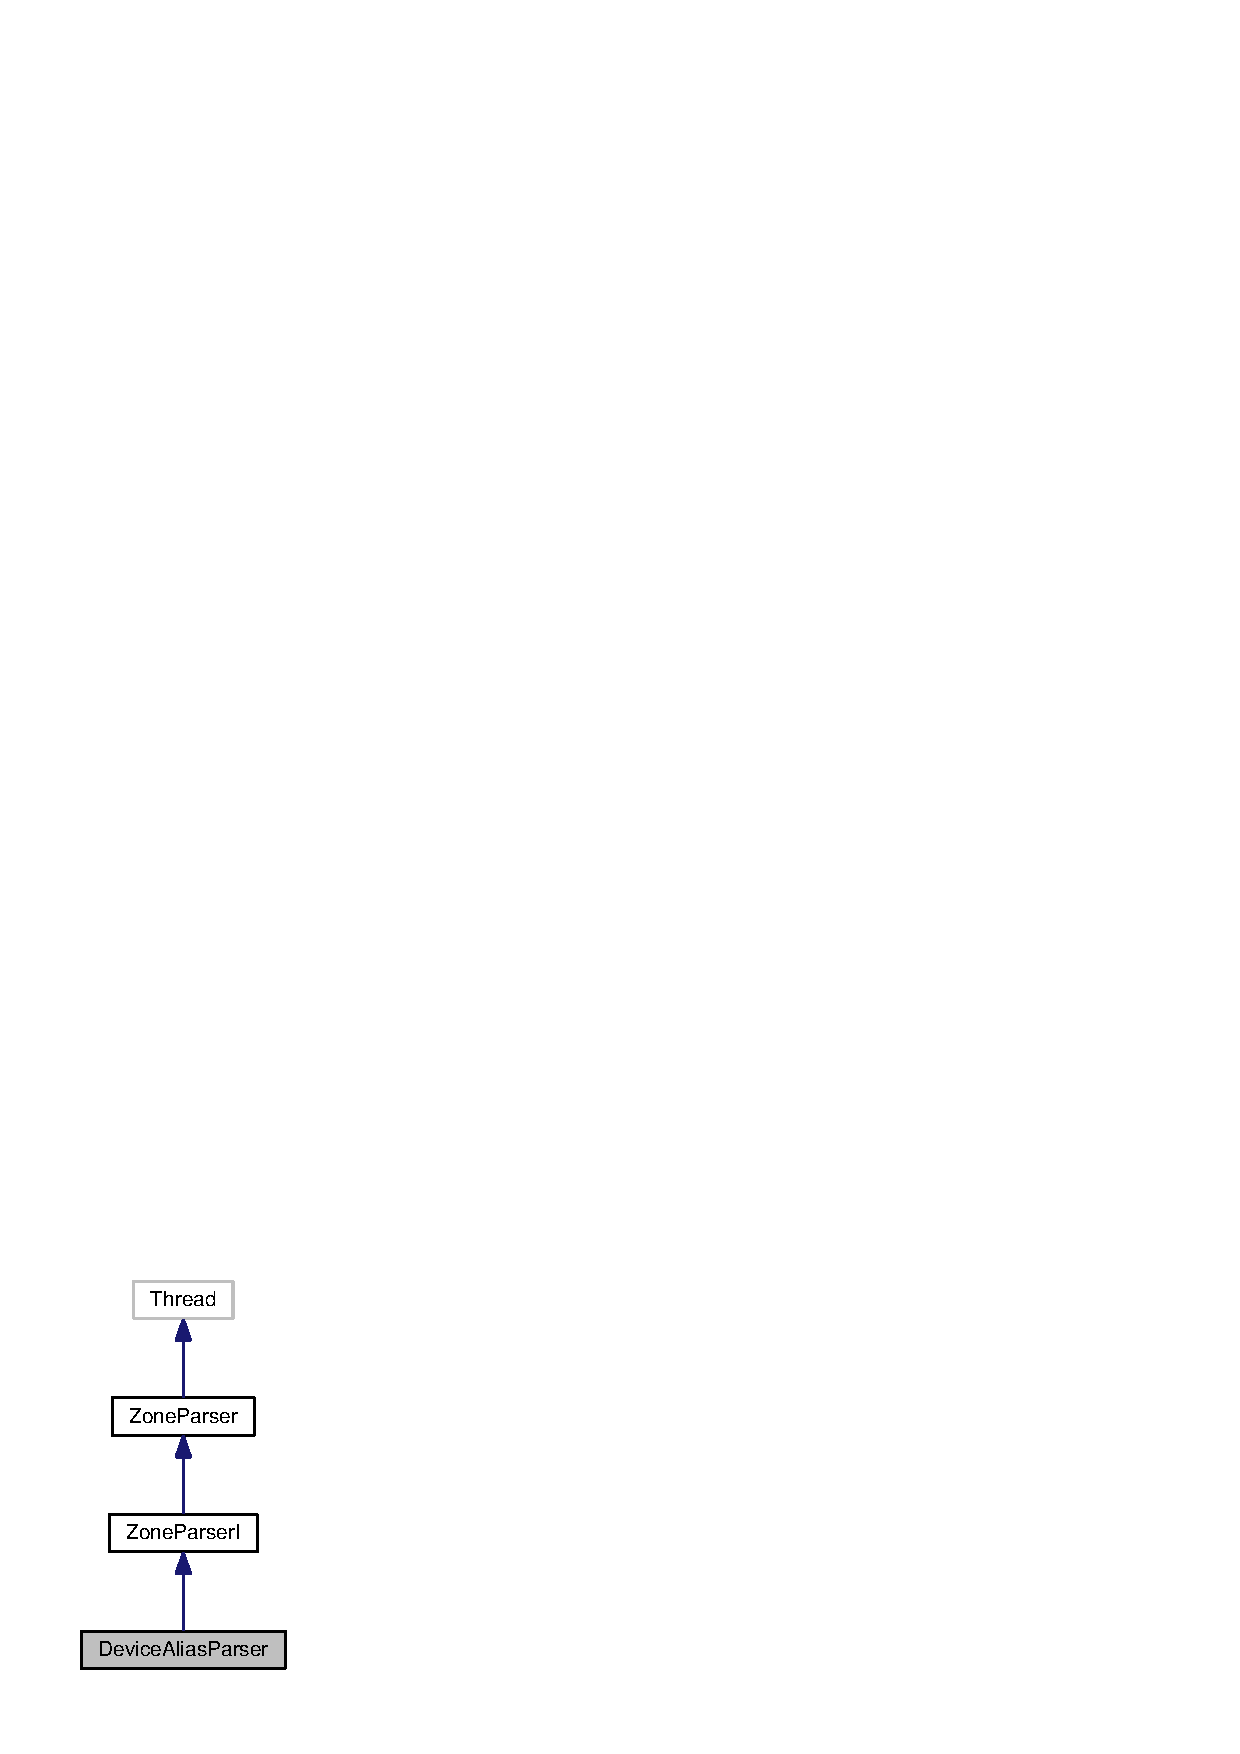
\includegraphics[width=140pt]{classorg_1_1smallfoot_1_1parser_1_1zone_1_1DeviceAliasParser__inherit__graph}
\end{center}
\end{figure}


Collaboration diagram for Device\-Alias\-Parser\-:\nopagebreak
\begin{figure}[H]
\begin{center}
\leavevmode
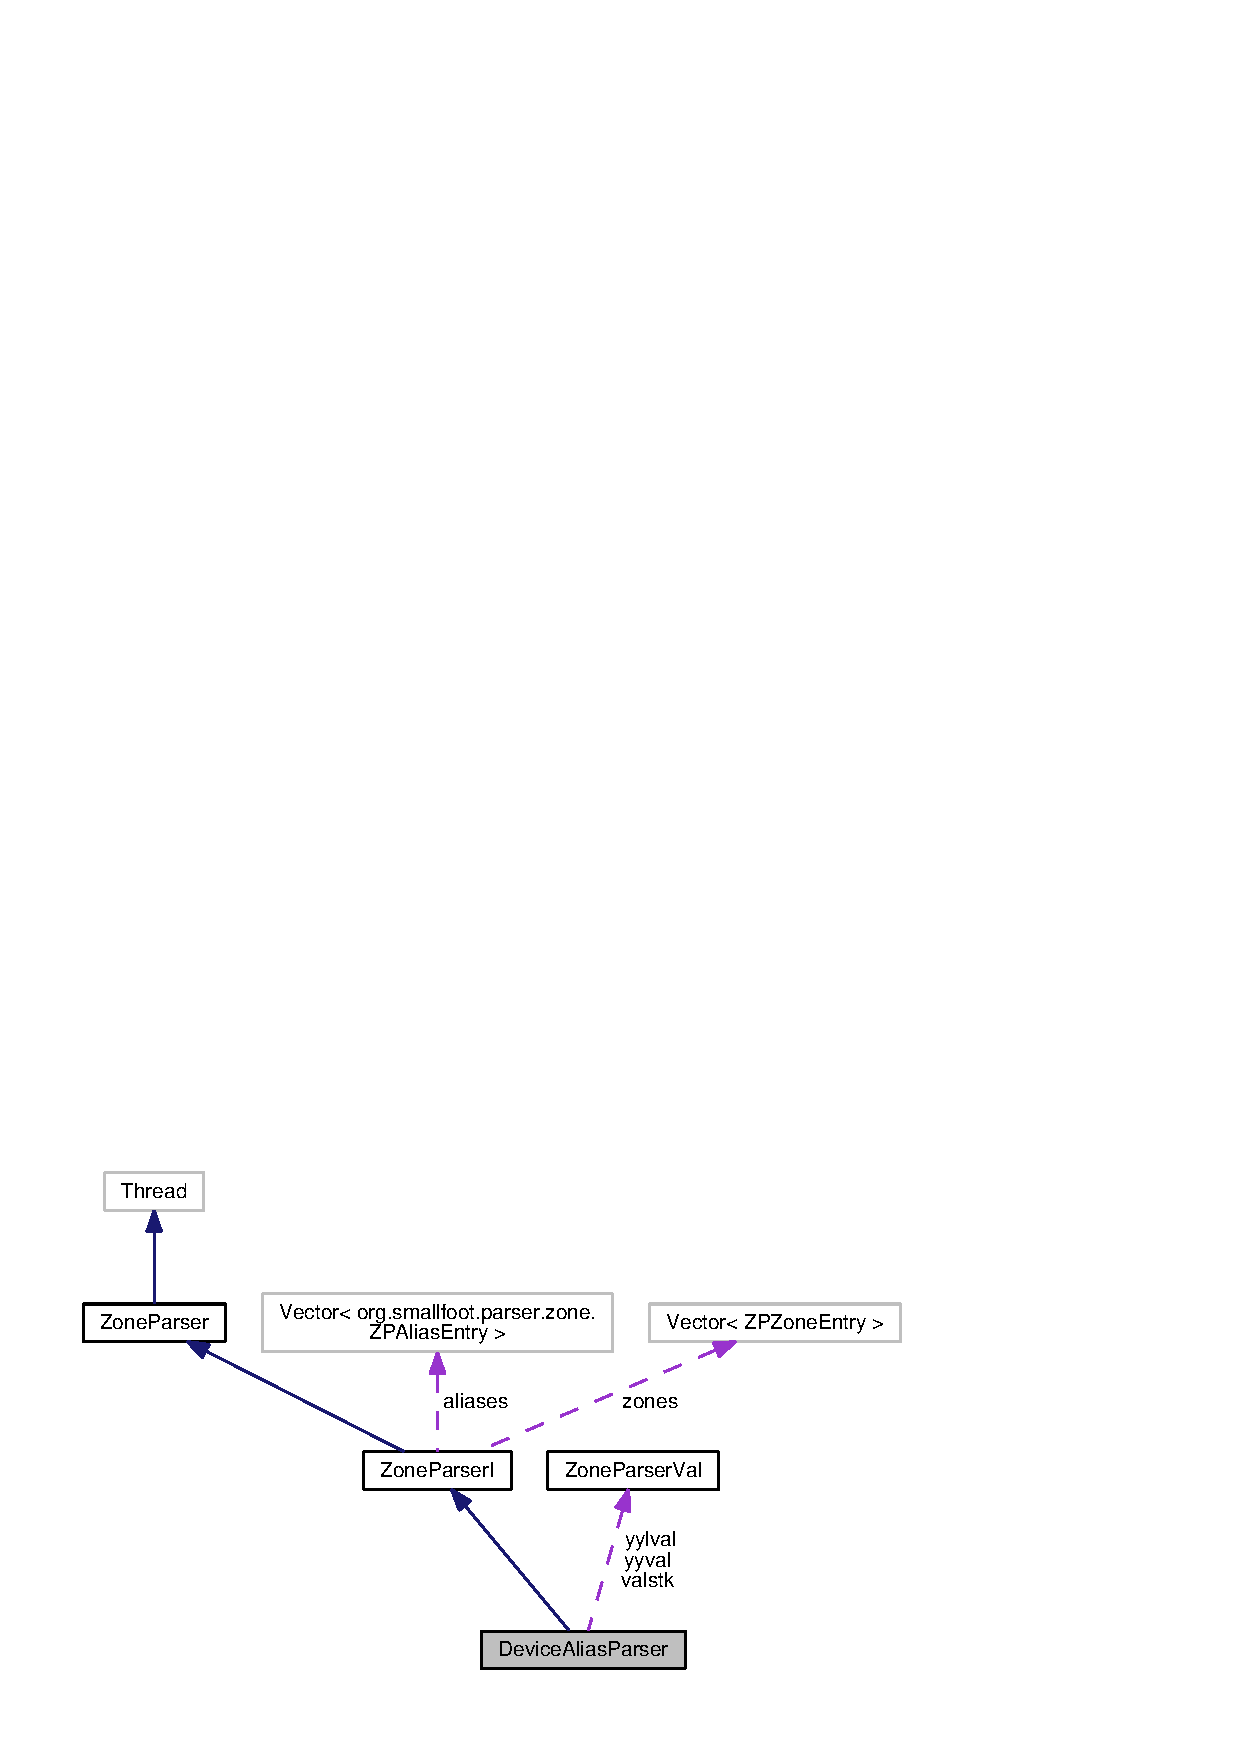
\includegraphics[width=213pt]{classorg_1_1smallfoot_1_1parser_1_1zone_1_1DeviceAliasParser__coll__graph}
\end{center}
\end{figure}
\subsection*{Public Member Functions}
\begin{DoxyCompactItemize}
\item 
void {\bf parse} ()
\item 
void {\bf set\-Reader} (Reader in)
\item 
void {\bf run} ()
\item 
void {\bf set\-Debug} (boolean debug)
\item 
{\bf Device\-Alias\-Parser} (Input\-Stream in, boolean debug\-Me)
\item 
{\bf Device\-Alias\-Parser} (java.\-util.\-Properties in, boolean debug\-Me)
\end{DoxyCompactItemize}
\subsection*{Static Public Member Functions}
\begin{DoxyCompactItemize}
\item 
static void {\bf main} (String args[$\,$])
\end{DoxyCompactItemize}
\subsection*{Static Public Attributes}
\begin{DoxyCompactItemize}
\item 
static final short {\bf D\-E\-V\-I\-C\-E\-A\-L\-I\-A\-S} =257
\item 
static final short {\bf N\-A\-M\-E} =258
\item 
static final short {\bf P\-W\-W\-N} =259
\item 
static final short {\bf A\-L\-P\-H\-A\-N\-U\-M} =260
\item 
static final short {\bf Y\-Y\-E\-R\-R\-C\-O\-D\-E} =256
\end{DoxyCompactItemize}


\subsection{Detailed Description}


Definition at line 29 of file Device\-Alias\-Parser.\-java.



\subsection{Constructor \& Destructor Documentation}
\index{org\-::smallfoot\-::parser\-::zone\-::\-Device\-Alias\-Parser@{org\-::smallfoot\-::parser\-::zone\-::\-Device\-Alias\-Parser}!Device\-Alias\-Parser@{Device\-Alias\-Parser}}
\index{Device\-Alias\-Parser@{Device\-Alias\-Parser}!org::smallfoot::parser::zone::DeviceAliasParser@{org\-::smallfoot\-::parser\-::zone\-::\-Device\-Alias\-Parser}}
\subsubsection[{Device\-Alias\-Parser}]{\setlength{\rightskip}{0pt plus 5cm}{\bf Device\-Alias\-Parser} (
\begin{DoxyParamCaption}
\item[{Input\-Stream}]{in, }
\item[{boolean}]{debug\-Me}
\end{DoxyParamCaption}
)\hspace{0.3cm}{\ttfamily [inline]}}\label{classorg_1_1smallfoot_1_1parser_1_1zone_1_1DeviceAliasParser_af519c80bc4449da0ad3d5e335175b967}


Definition at line 419 of file Device\-Alias\-Parser.\-java.



Referenced by Device\-Alias\-Parser.\-main().

\index{org\-::smallfoot\-::parser\-::zone\-::\-Device\-Alias\-Parser@{org\-::smallfoot\-::parser\-::zone\-::\-Device\-Alias\-Parser}!Device\-Alias\-Parser@{Device\-Alias\-Parser}}
\index{Device\-Alias\-Parser@{Device\-Alias\-Parser}!org::smallfoot::parser::zone::DeviceAliasParser@{org\-::smallfoot\-::parser\-::zone\-::\-Device\-Alias\-Parser}}
\subsubsection[{Device\-Alias\-Parser}]{\setlength{\rightskip}{0pt plus 5cm}{\bf Device\-Alias\-Parser} (
\begin{DoxyParamCaption}
\item[{java.\-util.\-Properties}]{in, }
\item[{boolean}]{debug\-Me}
\end{DoxyParamCaption}
)\hspace{0.3cm}{\ttfamily [inline]}}\label{classorg_1_1smallfoot_1_1parser_1_1zone_1_1DeviceAliasParser_a3ff85655cdcdba2cd8fa38166af469c0}


Definition at line 420 of file Device\-Alias\-Parser.\-java.



\subsection{Member Function Documentation}
\index{org\-::smallfoot\-::parser\-::zone\-::\-Device\-Alias\-Parser@{org\-::smallfoot\-::parser\-::zone\-::\-Device\-Alias\-Parser}!main@{main}}
\index{main@{main}!org::smallfoot::parser::zone::DeviceAliasParser@{org\-::smallfoot\-::parser\-::zone\-::\-Device\-Alias\-Parser}}
\subsubsection[{main}]{\setlength{\rightskip}{0pt plus 5cm}static void main (
\begin{DoxyParamCaption}
\item[{String}]{args[$\,$]}
\end{DoxyParamCaption}
)\hspace{0.3cm}{\ttfamily [inline]}, {\ttfamily [static]}}\label{classorg_1_1smallfoot_1_1parser_1_1zone_1_1DeviceAliasParser_a75988cf84fc6ee7a2ebff36e363021aa}


Definition at line 423 of file Device\-Alias\-Parser.\-java.



References Device\-Alias\-Parser.\-Device\-Alias\-Parser().



Here is the call graph for this function\-:\nopagebreak
\begin{figure}[H]
\begin{center}
\leavevmode
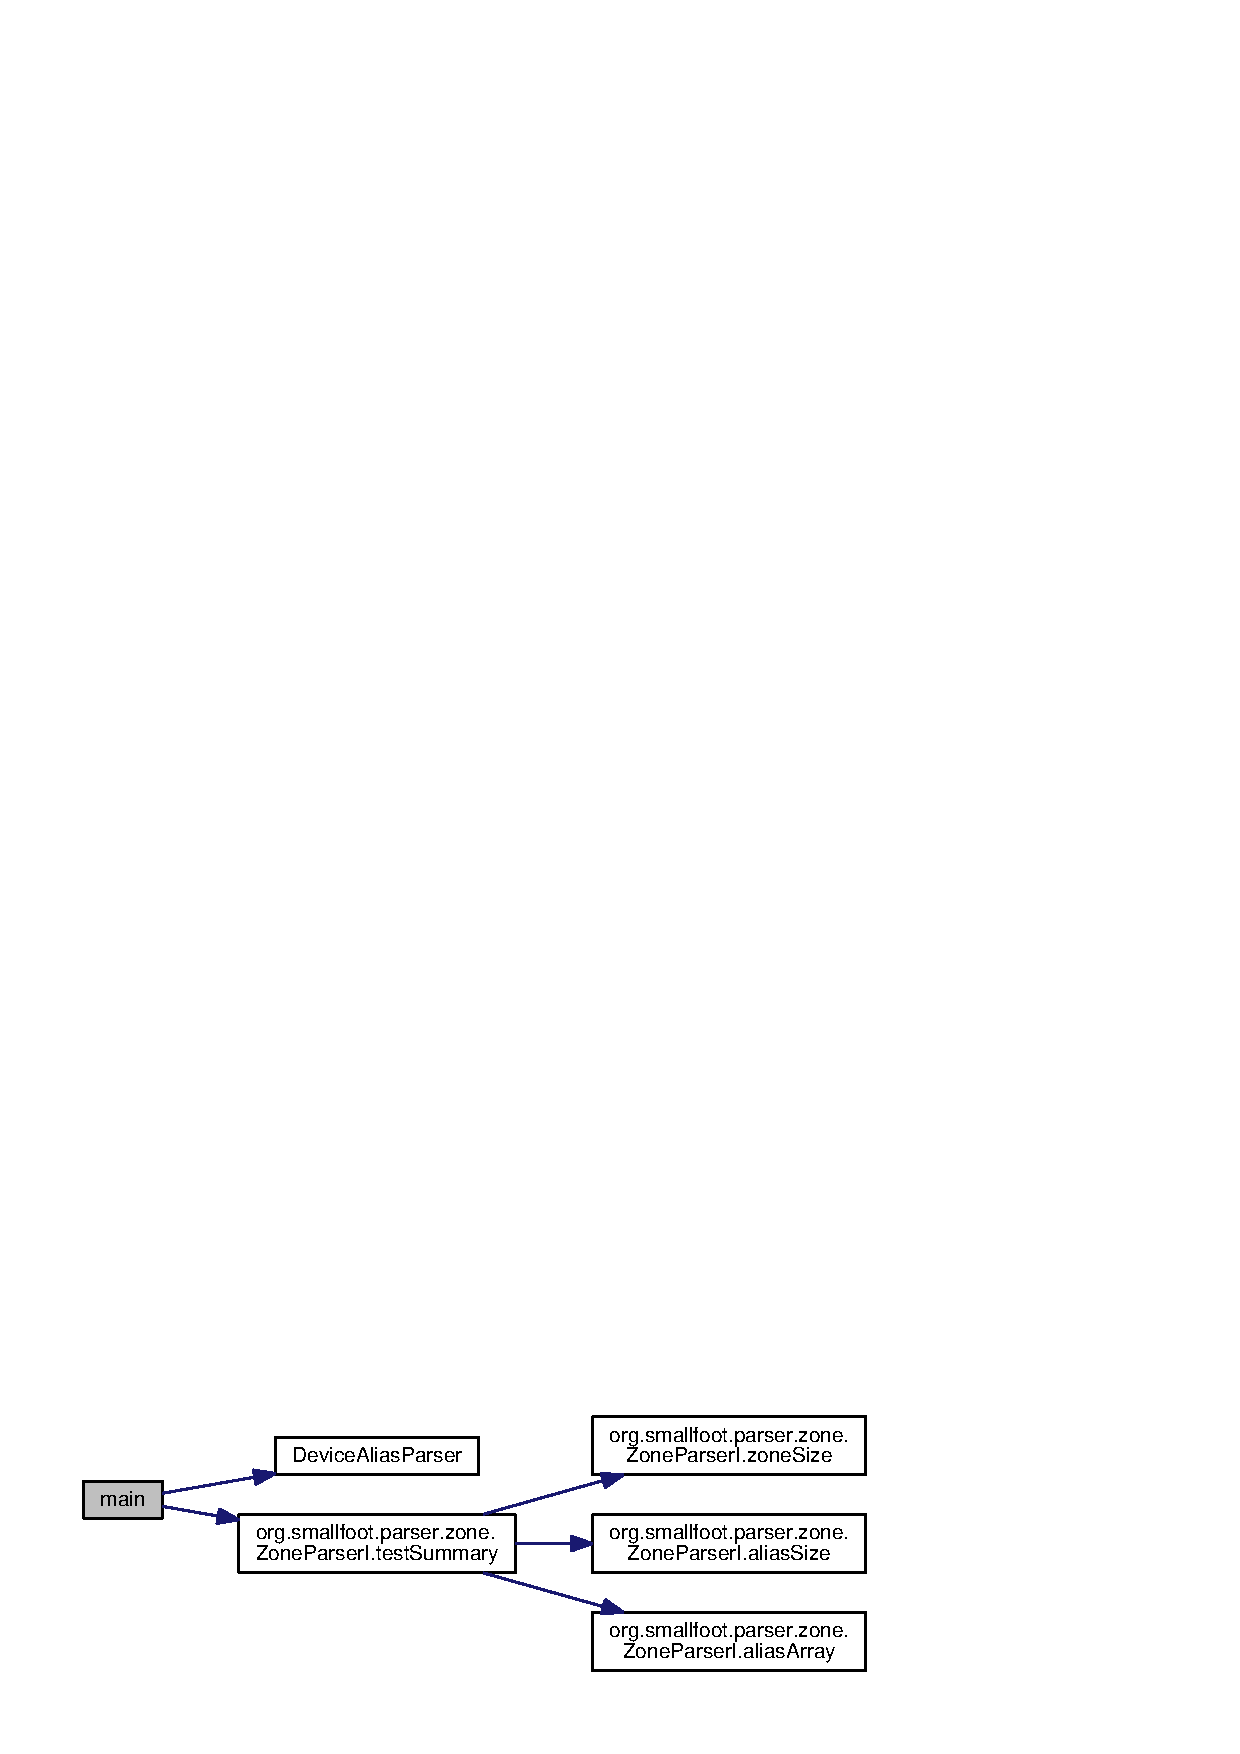
\includegraphics[width=216pt]{classorg_1_1smallfoot_1_1parser_1_1zone_1_1DeviceAliasParser_a75988cf84fc6ee7a2ebff36e363021aa_cgraph}
\end{center}
\end{figure}


\index{org\-::smallfoot\-::parser\-::zone\-::\-Device\-Alias\-Parser@{org\-::smallfoot\-::parser\-::zone\-::\-Device\-Alias\-Parser}!parse@{parse}}
\index{parse@{parse}!org::smallfoot::parser::zone::DeviceAliasParser@{org\-::smallfoot\-::parser\-::zone\-::\-Device\-Alias\-Parser}}
\subsubsection[{parse}]{\setlength{\rightskip}{0pt plus 5cm}void parse (
\begin{DoxyParamCaption}
{}
\end{DoxyParamCaption}
)\hspace{0.3cm}{\ttfamily [inline]}}\label{classorg_1_1smallfoot_1_1parser_1_1zone_1_1DeviceAliasParser_ad7c704b34912678d95c13243cacf9d7f}


Definition at line 362 of file Device\-Alias\-Parser.\-java.

\index{org\-::smallfoot\-::parser\-::zone\-::\-Device\-Alias\-Parser@{org\-::smallfoot\-::parser\-::zone\-::\-Device\-Alias\-Parser}!run@{run}}
\index{run@{run}!org::smallfoot::parser::zone::DeviceAliasParser@{org\-::smallfoot\-::parser\-::zone\-::\-Device\-Alias\-Parser}}
\subsubsection[{run}]{\setlength{\rightskip}{0pt plus 5cm}void run (
\begin{DoxyParamCaption}
{}
\end{DoxyParamCaption}
)\hspace{0.3cm}{\ttfamily [inline]}}\label{classorg_1_1smallfoot_1_1parser_1_1zone_1_1DeviceAliasParser_a13a43e6d814de94978c515cb084873b1}


Definition at line 406 of file Device\-Alias\-Parser.\-java.

\index{org\-::smallfoot\-::parser\-::zone\-::\-Device\-Alias\-Parser@{org\-::smallfoot\-::parser\-::zone\-::\-Device\-Alias\-Parser}!set\-Debug@{set\-Debug}}
\index{set\-Debug@{set\-Debug}!org::smallfoot::parser::zone::DeviceAliasParser@{org\-::smallfoot\-::parser\-::zone\-::\-Device\-Alias\-Parser}}
\subsubsection[{set\-Debug}]{\setlength{\rightskip}{0pt plus 5cm}void set\-Debug (
\begin{DoxyParamCaption}
\item[{boolean}]{debug}
\end{DoxyParamCaption}
)\hspace{0.3cm}{\ttfamily [inline]}}\label{classorg_1_1smallfoot_1_1parser_1_1zone_1_1DeviceAliasParser_a6c13d260cf71d0554f789c4641a9f18b}


Definition at line 417 of file Device\-Alias\-Parser.\-java.

\index{org\-::smallfoot\-::parser\-::zone\-::\-Device\-Alias\-Parser@{org\-::smallfoot\-::parser\-::zone\-::\-Device\-Alias\-Parser}!set\-Reader@{set\-Reader}}
\index{set\-Reader@{set\-Reader}!org::smallfoot::parser::zone::DeviceAliasParser@{org\-::smallfoot\-::parser\-::zone\-::\-Device\-Alias\-Parser}}
\subsubsection[{set\-Reader}]{\setlength{\rightskip}{0pt plus 5cm}void set\-Reader (
\begin{DoxyParamCaption}
\item[{Reader}]{in}
\end{DoxyParamCaption}
)\hspace{0.3cm}{\ttfamily [inline]}}\label{classorg_1_1smallfoot_1_1parser_1_1zone_1_1DeviceAliasParser_a5deab139f9ad4072e1a497c5cccda0ea}


Definition at line 374 of file Device\-Alias\-Parser.\-java.



\subsection{Field Documentation}
\index{org\-::smallfoot\-::parser\-::zone\-::\-Device\-Alias\-Parser@{org\-::smallfoot\-::parser\-::zone\-::\-Device\-Alias\-Parser}!A\-L\-P\-H\-A\-N\-U\-M@{A\-L\-P\-H\-A\-N\-U\-M}}
\index{A\-L\-P\-H\-A\-N\-U\-M@{A\-L\-P\-H\-A\-N\-U\-M}!org::smallfoot::parser::zone::DeviceAliasParser@{org\-::smallfoot\-::parser\-::zone\-::\-Device\-Alias\-Parser}}
\subsubsection[{A\-L\-P\-H\-A\-N\-U\-M}]{\setlength{\rightskip}{0pt plus 5cm}final short A\-L\-P\-H\-A\-N\-U\-M =260\hspace{0.3cm}{\ttfamily [static]}}\label{classorg_1_1smallfoot_1_1parser_1_1zone_1_1DeviceAliasParser_afa1bd945463851953be939c8793faf70}


Definition at line 157 of file Device\-Alias\-Parser.\-java.

\index{org\-::smallfoot\-::parser\-::zone\-::\-Device\-Alias\-Parser@{org\-::smallfoot\-::parser\-::zone\-::\-Device\-Alias\-Parser}!D\-E\-V\-I\-C\-E\-A\-L\-I\-A\-S@{D\-E\-V\-I\-C\-E\-A\-L\-I\-A\-S}}
\index{D\-E\-V\-I\-C\-E\-A\-L\-I\-A\-S@{D\-E\-V\-I\-C\-E\-A\-L\-I\-A\-S}!org::smallfoot::parser::zone::DeviceAliasParser@{org\-::smallfoot\-::parser\-::zone\-::\-Device\-Alias\-Parser}}
\subsubsection[{D\-E\-V\-I\-C\-E\-A\-L\-I\-A\-S}]{\setlength{\rightskip}{0pt plus 5cm}final short D\-E\-V\-I\-C\-E\-A\-L\-I\-A\-S =257\hspace{0.3cm}{\ttfamily [static]}}\label{classorg_1_1smallfoot_1_1parser_1_1zone_1_1DeviceAliasParser_acabf8c32cf826e213b6e287fd5c70001}


Definition at line 154 of file Device\-Alias\-Parser.\-java.

\index{org\-::smallfoot\-::parser\-::zone\-::\-Device\-Alias\-Parser@{org\-::smallfoot\-::parser\-::zone\-::\-Device\-Alias\-Parser}!N\-A\-M\-E@{N\-A\-M\-E}}
\index{N\-A\-M\-E@{N\-A\-M\-E}!org::smallfoot::parser::zone::DeviceAliasParser@{org\-::smallfoot\-::parser\-::zone\-::\-Device\-Alias\-Parser}}
\subsubsection[{N\-A\-M\-E}]{\setlength{\rightskip}{0pt plus 5cm}final short N\-A\-M\-E =258\hspace{0.3cm}{\ttfamily [static]}}\label{classorg_1_1smallfoot_1_1parser_1_1zone_1_1DeviceAliasParser_a66fe0c51d242ca6db52c31bf73a55f8e}


Definition at line 155 of file Device\-Alias\-Parser.\-java.

\index{org\-::smallfoot\-::parser\-::zone\-::\-Device\-Alias\-Parser@{org\-::smallfoot\-::parser\-::zone\-::\-Device\-Alias\-Parser}!P\-W\-W\-N@{P\-W\-W\-N}}
\index{P\-W\-W\-N@{P\-W\-W\-N}!org::smallfoot::parser::zone::DeviceAliasParser@{org\-::smallfoot\-::parser\-::zone\-::\-Device\-Alias\-Parser}}
\subsubsection[{P\-W\-W\-N}]{\setlength{\rightskip}{0pt plus 5cm}final short P\-W\-W\-N =259\hspace{0.3cm}{\ttfamily [static]}}\label{classorg_1_1smallfoot_1_1parser_1_1zone_1_1DeviceAliasParser_aaa70cc94f40a0785c0ce9ce3cf2ff61d}


Definition at line 156 of file Device\-Alias\-Parser.\-java.

\index{org\-::smallfoot\-::parser\-::zone\-::\-Device\-Alias\-Parser@{org\-::smallfoot\-::parser\-::zone\-::\-Device\-Alias\-Parser}!Y\-Y\-E\-R\-R\-C\-O\-D\-E@{Y\-Y\-E\-R\-R\-C\-O\-D\-E}}
\index{Y\-Y\-E\-R\-R\-C\-O\-D\-E@{Y\-Y\-E\-R\-R\-C\-O\-D\-E}!org::smallfoot::parser::zone::DeviceAliasParser@{org\-::smallfoot\-::parser\-::zone\-::\-Device\-Alias\-Parser}}
\subsubsection[{Y\-Y\-E\-R\-R\-C\-O\-D\-E}]{\setlength{\rightskip}{0pt plus 5cm}final short Y\-Y\-E\-R\-R\-C\-O\-D\-E =256\hspace{0.3cm}{\ttfamily [static]}}\label{classorg_1_1smallfoot_1_1parser_1_1zone_1_1DeviceAliasParser_a1c58472ea6621d2f613831e08d10dba3}


Definition at line 158 of file Device\-Alias\-Parser.\-java.



The documentation for this class was generated from the following file\-:\begin{DoxyCompactItemize}
\item 
java/{\bf Device\-Alias\-Parser.\-java}\end{DoxyCompactItemize}

\section{Z\+P\+Alias\+Entry.\+Device\+Type Enum Reference}
\label{enumorg_1_1smallfoot_1_1parser_1_1zone_1_1ZPAliasEntry_1_1DeviceType}\index{Z\+P\+Alias\+Entry.\+Device\+Type@{Z\+P\+Alias\+Entry.\+Device\+Type}}
\subsection*{Data Fields}
\begin{DoxyCompactItemize}
\item 
{\bf D\+E\+V\+\_\+\+U\+N\+K\+N\+O\+W\+N}
\item 
{\bf D\+E\+V\+\_\+\+S\+E\+R\+V\+E\+R}
\item 
{\bf D\+E\+V\+\_\+\+S\+W\+I\+T\+C\+H}
\item 
{\bf D\+E\+V\+\_\+\+S\+T\+O\+R\+A\+G\+E}
\item 
{\bf D\+E\+V\+\_\+\+T\+A\+P\+E}
\item 
{\bf D\+E\+V\+\_\+\+V\+I\+R\+T\+U\+A\+L\+I\+Z\+E\+R}
\item 
{\bf D\+E\+V\+\_\+\+O\+T\+H\+E\+R}
\end{DoxyCompactItemize}


\subsection{Detailed Description}


Definition at line 6 of file Z\+P\+Alias\+Entry.\+java.



\subsection{Field Documentation}
\index{org\+::smallfoot\+::parser\+::zone\+::\+Z\+P\+Alias\+Entry\+::\+Device\+Type@{org\+::smallfoot\+::parser\+::zone\+::\+Z\+P\+Alias\+Entry\+::\+Device\+Type}!D\+E\+V\+\_\+\+O\+T\+H\+E\+R@{D\+E\+V\+\_\+\+O\+T\+H\+E\+R}}
\index{D\+E\+V\+\_\+\+O\+T\+H\+E\+R@{D\+E\+V\+\_\+\+O\+T\+H\+E\+R}!org\+::smallfoot\+::parser\+::zone\+::\+Z\+P\+Alias\+Entry\+::\+Device\+Type@{org\+::smallfoot\+::parser\+::zone\+::\+Z\+P\+Alias\+Entry\+::\+Device\+Type}}
\subsubsection[{D\+E\+V\+\_\+\+O\+T\+H\+E\+R}]{\setlength{\rightskip}{0pt plus 5cm}D\+E\+V\+\_\+\+O\+T\+H\+E\+R}\label{enumorg_1_1smallfoot_1_1parser_1_1zone_1_1ZPAliasEntry_1_1DeviceType_a16792ac0d619df5babc1a94c7a0296ff}


Definition at line 6 of file Z\+P\+Alias\+Entry.\+java.

\index{org\+::smallfoot\+::parser\+::zone\+::\+Z\+P\+Alias\+Entry\+::\+Device\+Type@{org\+::smallfoot\+::parser\+::zone\+::\+Z\+P\+Alias\+Entry\+::\+Device\+Type}!D\+E\+V\+\_\+\+S\+E\+R\+V\+E\+R@{D\+E\+V\+\_\+\+S\+E\+R\+V\+E\+R}}
\index{D\+E\+V\+\_\+\+S\+E\+R\+V\+E\+R@{D\+E\+V\+\_\+\+S\+E\+R\+V\+E\+R}!org\+::smallfoot\+::parser\+::zone\+::\+Z\+P\+Alias\+Entry\+::\+Device\+Type@{org\+::smallfoot\+::parser\+::zone\+::\+Z\+P\+Alias\+Entry\+::\+Device\+Type}}
\subsubsection[{D\+E\+V\+\_\+\+S\+E\+R\+V\+E\+R}]{\setlength{\rightskip}{0pt plus 5cm}D\+E\+V\+\_\+\+S\+E\+R\+V\+E\+R}\label{enumorg_1_1smallfoot_1_1parser_1_1zone_1_1ZPAliasEntry_1_1DeviceType_a2a5477499e7cc4af0a446cafc2fdff69}


Definition at line 6 of file Z\+P\+Alias\+Entry.\+java.

\index{org\+::smallfoot\+::parser\+::zone\+::\+Z\+P\+Alias\+Entry\+::\+Device\+Type@{org\+::smallfoot\+::parser\+::zone\+::\+Z\+P\+Alias\+Entry\+::\+Device\+Type}!D\+E\+V\+\_\+\+S\+T\+O\+R\+A\+G\+E@{D\+E\+V\+\_\+\+S\+T\+O\+R\+A\+G\+E}}
\index{D\+E\+V\+\_\+\+S\+T\+O\+R\+A\+G\+E@{D\+E\+V\+\_\+\+S\+T\+O\+R\+A\+G\+E}!org\+::smallfoot\+::parser\+::zone\+::\+Z\+P\+Alias\+Entry\+::\+Device\+Type@{org\+::smallfoot\+::parser\+::zone\+::\+Z\+P\+Alias\+Entry\+::\+Device\+Type}}
\subsubsection[{D\+E\+V\+\_\+\+S\+T\+O\+R\+A\+G\+E}]{\setlength{\rightskip}{0pt plus 5cm}D\+E\+V\+\_\+\+S\+T\+O\+R\+A\+G\+E}\label{enumorg_1_1smallfoot_1_1parser_1_1zone_1_1ZPAliasEntry_1_1DeviceType_a3ee32b644cbbba8e614f55c2d9952701}


Definition at line 6 of file Z\+P\+Alias\+Entry.\+java.

\index{org\+::smallfoot\+::parser\+::zone\+::\+Z\+P\+Alias\+Entry\+::\+Device\+Type@{org\+::smallfoot\+::parser\+::zone\+::\+Z\+P\+Alias\+Entry\+::\+Device\+Type}!D\+E\+V\+\_\+\+S\+W\+I\+T\+C\+H@{D\+E\+V\+\_\+\+S\+W\+I\+T\+C\+H}}
\index{D\+E\+V\+\_\+\+S\+W\+I\+T\+C\+H@{D\+E\+V\+\_\+\+S\+W\+I\+T\+C\+H}!org\+::smallfoot\+::parser\+::zone\+::\+Z\+P\+Alias\+Entry\+::\+Device\+Type@{org\+::smallfoot\+::parser\+::zone\+::\+Z\+P\+Alias\+Entry\+::\+Device\+Type}}
\subsubsection[{D\+E\+V\+\_\+\+S\+W\+I\+T\+C\+H}]{\setlength{\rightskip}{0pt plus 5cm}D\+E\+V\+\_\+\+S\+W\+I\+T\+C\+H}\label{enumorg_1_1smallfoot_1_1parser_1_1zone_1_1ZPAliasEntry_1_1DeviceType_a066e9d3aa3023aa6377f20e41874727d}


Definition at line 6 of file Z\+P\+Alias\+Entry.\+java.

\index{org\+::smallfoot\+::parser\+::zone\+::\+Z\+P\+Alias\+Entry\+::\+Device\+Type@{org\+::smallfoot\+::parser\+::zone\+::\+Z\+P\+Alias\+Entry\+::\+Device\+Type}!D\+E\+V\+\_\+\+T\+A\+P\+E@{D\+E\+V\+\_\+\+T\+A\+P\+E}}
\index{D\+E\+V\+\_\+\+T\+A\+P\+E@{D\+E\+V\+\_\+\+T\+A\+P\+E}!org\+::smallfoot\+::parser\+::zone\+::\+Z\+P\+Alias\+Entry\+::\+Device\+Type@{org\+::smallfoot\+::parser\+::zone\+::\+Z\+P\+Alias\+Entry\+::\+Device\+Type}}
\subsubsection[{D\+E\+V\+\_\+\+T\+A\+P\+E}]{\setlength{\rightskip}{0pt plus 5cm}D\+E\+V\+\_\+\+T\+A\+P\+E}\label{enumorg_1_1smallfoot_1_1parser_1_1zone_1_1ZPAliasEntry_1_1DeviceType_acc26107efaf346173b211684eb2b580a}


Definition at line 6 of file Z\+P\+Alias\+Entry.\+java.

\index{org\+::smallfoot\+::parser\+::zone\+::\+Z\+P\+Alias\+Entry\+::\+Device\+Type@{org\+::smallfoot\+::parser\+::zone\+::\+Z\+P\+Alias\+Entry\+::\+Device\+Type}!D\+E\+V\+\_\+\+U\+N\+K\+N\+O\+W\+N@{D\+E\+V\+\_\+\+U\+N\+K\+N\+O\+W\+N}}
\index{D\+E\+V\+\_\+\+U\+N\+K\+N\+O\+W\+N@{D\+E\+V\+\_\+\+U\+N\+K\+N\+O\+W\+N}!org\+::smallfoot\+::parser\+::zone\+::\+Z\+P\+Alias\+Entry\+::\+Device\+Type@{org\+::smallfoot\+::parser\+::zone\+::\+Z\+P\+Alias\+Entry\+::\+Device\+Type}}
\subsubsection[{D\+E\+V\+\_\+\+U\+N\+K\+N\+O\+W\+N}]{\setlength{\rightskip}{0pt plus 5cm}D\+E\+V\+\_\+\+U\+N\+K\+N\+O\+W\+N}\label{enumorg_1_1smallfoot_1_1parser_1_1zone_1_1ZPAliasEntry_1_1DeviceType_a2181504f7419b379d8107fa76cf98cc6}


Definition at line 6 of file Z\+P\+Alias\+Entry.\+java.

\index{org\+::smallfoot\+::parser\+::zone\+::\+Z\+P\+Alias\+Entry\+::\+Device\+Type@{org\+::smallfoot\+::parser\+::zone\+::\+Z\+P\+Alias\+Entry\+::\+Device\+Type}!D\+E\+V\+\_\+\+V\+I\+R\+T\+U\+A\+L\+I\+Z\+E\+R@{D\+E\+V\+\_\+\+V\+I\+R\+T\+U\+A\+L\+I\+Z\+E\+R}}
\index{D\+E\+V\+\_\+\+V\+I\+R\+T\+U\+A\+L\+I\+Z\+E\+R@{D\+E\+V\+\_\+\+V\+I\+R\+T\+U\+A\+L\+I\+Z\+E\+R}!org\+::smallfoot\+::parser\+::zone\+::\+Z\+P\+Alias\+Entry\+::\+Device\+Type@{org\+::smallfoot\+::parser\+::zone\+::\+Z\+P\+Alias\+Entry\+::\+Device\+Type}}
\subsubsection[{D\+E\+V\+\_\+\+V\+I\+R\+T\+U\+A\+L\+I\+Z\+E\+R}]{\setlength{\rightskip}{0pt plus 5cm}D\+E\+V\+\_\+\+V\+I\+R\+T\+U\+A\+L\+I\+Z\+E\+R}\label{enumorg_1_1smallfoot_1_1parser_1_1zone_1_1ZPAliasEntry_1_1DeviceType_a9e86c3fd05c684d8834cccae3c0f0ca1}


Definition at line 6 of file Z\+P\+Alias\+Entry.\+java.



The documentation for this enum was generated from the following file\+:\begin{DoxyCompactItemize}
\item 
java/{\bf Z\+P\+Alias\+Entry.\+java}\end{DoxyCompactItemize}

\section{D\+W\+H\+U\+R\+L\+Connection Class Reference}
\label{classorg_1_1smallfoot_1_1parser_1_1ocidwh_1_1DWHURLConnection}\index{D\+W\+H\+U\+R\+L\+Connection@{D\+W\+H\+U\+R\+L\+Connection}}


Inheritance diagram for D\+W\+H\+U\+R\+L\+Connection\+:\nopagebreak
\begin{figure}[H]
\begin{center}
\leavevmode
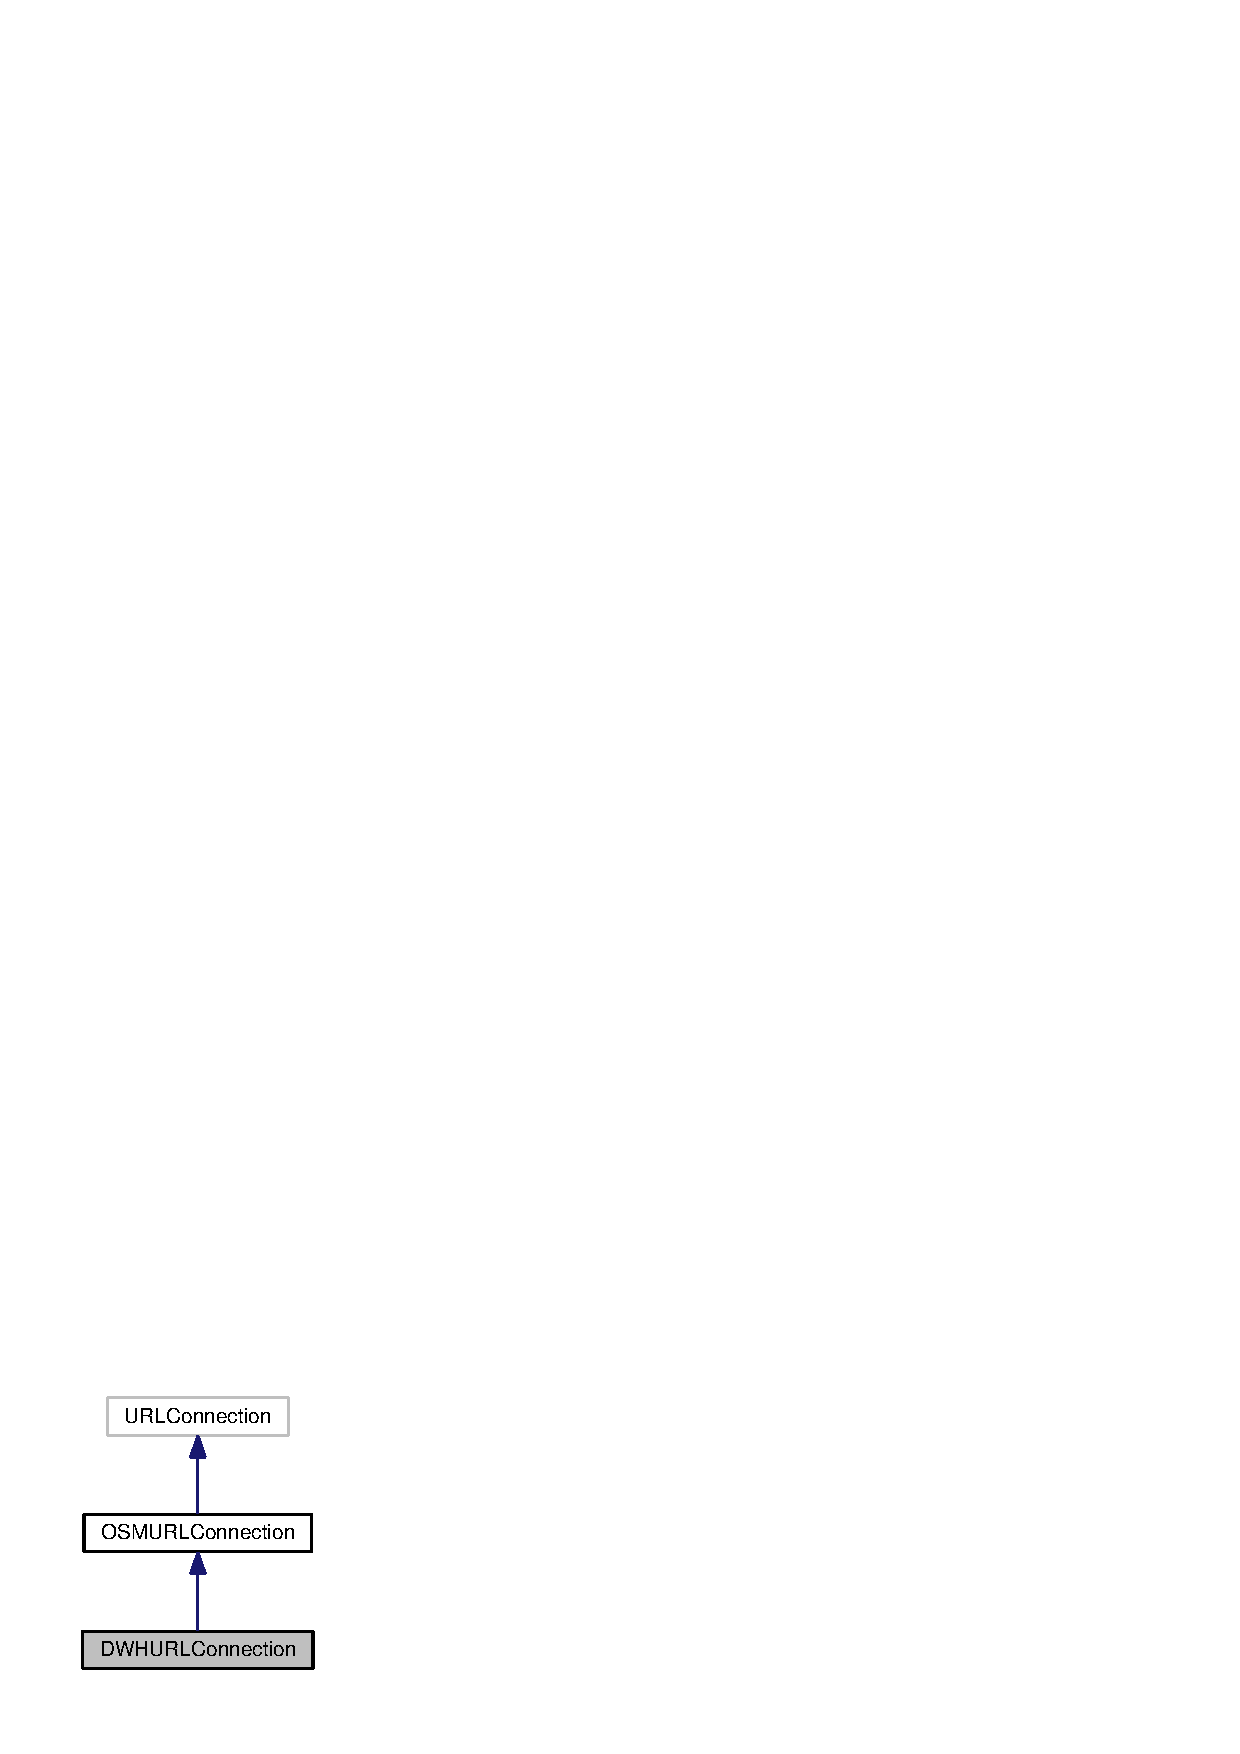
\includegraphics[width=154pt]{classorg_1_1smallfoot_1_1parser_1_1ocidwh_1_1DWHURLConnection__inherit__graph}
\end{center}
\end{figure}


Collaboration diagram for D\+W\+H\+U\+R\+L\+Connection\+:\nopagebreak
\begin{figure}[H]
\begin{center}
\leavevmode
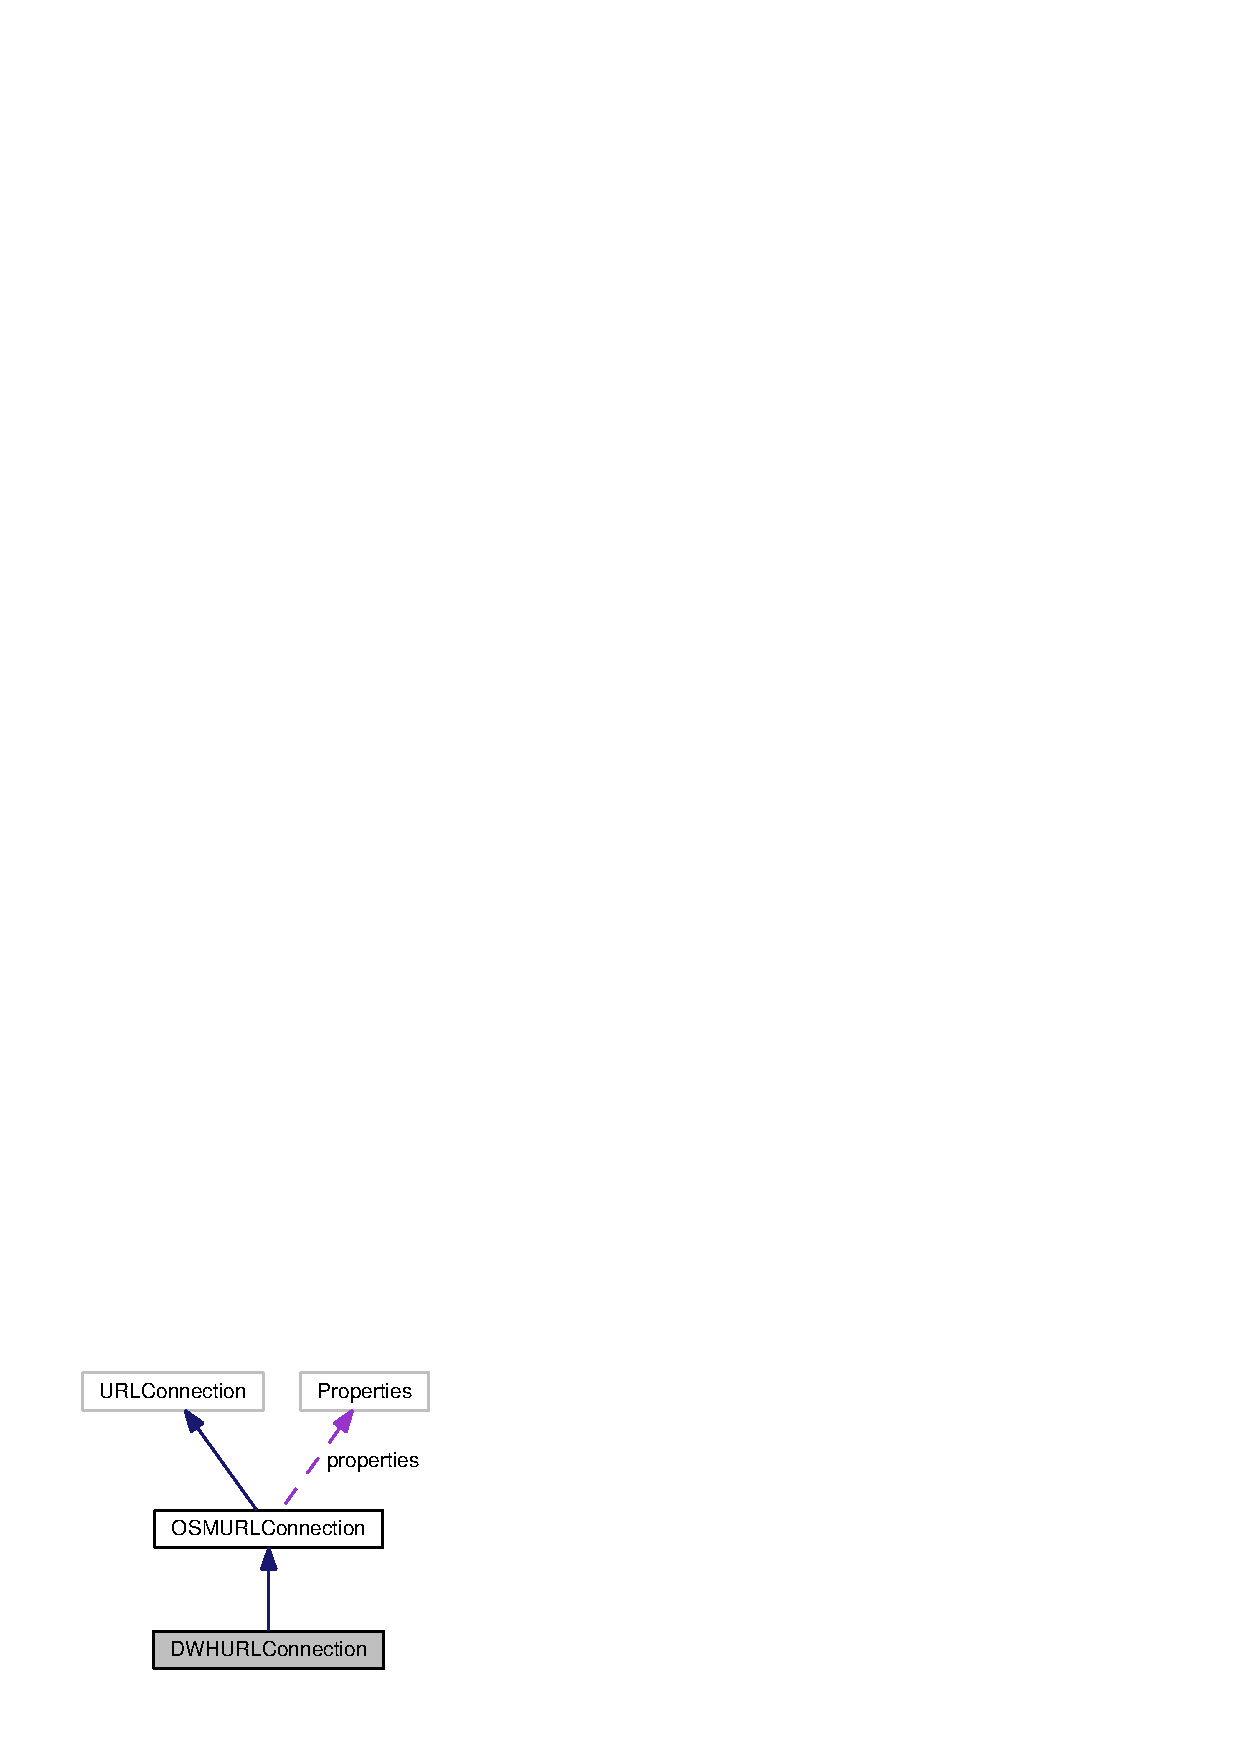
\includegraphics[width=209pt]{classorg_1_1smallfoot_1_1parser_1_1ocidwh_1_1DWHURLConnection__coll__graph}
\end{center}
\end{figure}
\subsection*{Public Member Functions}
\begin{DoxyCompactItemize}
\item 
{\bf D\+W\+H\+U\+R\+L\+Connection} (String connection\+Info, String username, String password)
\item 
{\bf D\+W\+H\+U\+R\+L\+Connection} (java.\+net.\+U\+R\+L url)
\end{DoxyCompactItemize}
\subsection*{Additional Inherited Members}


\subsection{Detailed Description}


Definition at line 24 of file D\+W\+H\+U\+R\+L\+Connection.\+java.



\subsection{Constructor \& Destructor Documentation}
\index{org\+::smallfoot\+::parser\+::ocidwh\+::\+D\+W\+H\+U\+R\+L\+Connection@{org\+::smallfoot\+::parser\+::ocidwh\+::\+D\+W\+H\+U\+R\+L\+Connection}!D\+W\+H\+U\+R\+L\+Connection@{D\+W\+H\+U\+R\+L\+Connection}}
\index{D\+W\+H\+U\+R\+L\+Connection@{D\+W\+H\+U\+R\+L\+Connection}!org\+::smallfoot\+::parser\+::ocidwh\+::\+D\+W\+H\+U\+R\+L\+Connection@{org\+::smallfoot\+::parser\+::ocidwh\+::\+D\+W\+H\+U\+R\+L\+Connection}}
\subsubsection[{D\+W\+H\+U\+R\+L\+Connection}]{\setlength{\rightskip}{0pt plus 5cm}{\bf D\+W\+H\+U\+R\+L\+Connection} (
\begin{DoxyParamCaption}
\item[{String}]{connection\+Info, }
\item[{String}]{username, }
\item[{String}]{password}
\end{DoxyParamCaption}
)\hspace{0.3cm}{\ttfamily [inline]}}\label{classorg_1_1smallfoot_1_1parser_1_1ocidwh_1_1DWHURLConnection_a88014571c73a1e1c9460c6cdb477377a}


Definition at line 26 of file D\+W\+H\+U\+R\+L\+Connection.\+java.

\index{org\+::smallfoot\+::parser\+::ocidwh\+::\+D\+W\+H\+U\+R\+L\+Connection@{org\+::smallfoot\+::parser\+::ocidwh\+::\+D\+W\+H\+U\+R\+L\+Connection}!D\+W\+H\+U\+R\+L\+Connection@{D\+W\+H\+U\+R\+L\+Connection}}
\index{D\+W\+H\+U\+R\+L\+Connection@{D\+W\+H\+U\+R\+L\+Connection}!org\+::smallfoot\+::parser\+::ocidwh\+::\+D\+W\+H\+U\+R\+L\+Connection@{org\+::smallfoot\+::parser\+::ocidwh\+::\+D\+W\+H\+U\+R\+L\+Connection}}
\subsubsection[{D\+W\+H\+U\+R\+L\+Connection}]{\setlength{\rightskip}{0pt plus 5cm}{\bf D\+W\+H\+U\+R\+L\+Connection} (
\begin{DoxyParamCaption}
\item[{java.\+net.\+U\+R\+L}]{url}
\end{DoxyParamCaption}
)\hspace{0.3cm}{\ttfamily [inline]}}\label{classorg_1_1smallfoot_1_1parser_1_1ocidwh_1_1DWHURLConnection_aba004da75ce33b0d07d5a0d2544f0f08}


Definition at line 31 of file D\+W\+H\+U\+R\+L\+Connection.\+java.



The documentation for this class was generated from the following file\+:\begin{DoxyCompactItemize}
\item 
java/{\bf D\+W\+H\+U\+R\+L\+Connection.\+java}\end{DoxyCompactItemize}

\section{F\+C\+Parser Class Reference}
\label{classorg_1_1smallfoot_1_1parser_1_1FCParser}\index{F\+C\+Parser@{F\+C\+Parser}}
\subsection*{Static Public Member Functions}
\begin{DoxyCompactItemize}
\item 
static java.\+io.\+Input\+Stream {\bf open\+Stream} (String uri)  throws java.\+io.\+File\+Not\+Found\+Exception, java.\+net.\+Malformed\+U\+R\+L\+Exception, java.\+io.\+I\+O\+Exception     
\begin{DoxyCompactList}\small\item\em Produce an Input\+Stream for the given uri in a way that corresponds to the url protocol. \end{DoxyCompactList}\item 
static void {\bf register\+Protocols} ()
\begin{DoxyCompactList}\small\item\em Collect in a single place the process to register protocol handlers. \end{DoxyCompactList}\item 
static Input\+Stream {\bf open\+Source} (String url, boolean verbose, java.\+util.\+Properties prop)
\begin{DoxyCompactList}\small\item\em Create a stream from a U\+R\+L or file name with a convenience workaround for no-\/proto U\+R\+Ls. \end{DoxyCompactList}\item 
static {\bf Zone\+Parser} {\bf load\+File} (Input\+Stream is, String args0, boolean verbose, java.\+util.\+Properties prop)
\begin{DoxyCompactList}\small\item\em Load a file from the resource given to a W\+W\+N/\+Nickname vector. \end{DoxyCompactList}\item 
static void {\bf main} (String args[$\,$])
\begin{DoxyCompactList}\small\item\em Main function, as you can tell. \end{DoxyCompactList}\end{DoxyCompactItemize}


\subsection{Detailed Description}


Definition at line 29 of file F\+C\+Parser.\+java.



\subsection{Member Function Documentation}
\index{org\+::smallfoot\+::parser\+::\+F\+C\+Parser@{org\+::smallfoot\+::parser\+::\+F\+C\+Parser}!load\+File@{load\+File}}
\index{load\+File@{load\+File}!org\+::smallfoot\+::parser\+::\+F\+C\+Parser@{org\+::smallfoot\+::parser\+::\+F\+C\+Parser}}
\subsubsection[{load\+File}]{\setlength{\rightskip}{0pt plus 5cm}static {\bf Zone\+Parser} load\+File (
\begin{DoxyParamCaption}
\item[{Input\+Stream}]{is, }
\item[{String}]{args0, }
\item[{boolean}]{verbose, }
\item[{java.\+util.\+Properties}]{prop}
\end{DoxyParamCaption}
)\hspace{0.3cm}{\ttfamily [inline]}, {\ttfamily [static]}}\label{classorg_1_1smallfoot_1_1parser_1_1FCParser_a47b0fe73f5a3ae8d0b5e23da3b1b4b63}


Load a file from the resource given to a W\+W\+N/\+Nickname vector. 

\begin{DoxyReturn}{Returns}
the number of things loaded (used to trigger obsessive retries to get around choking org.\+apache.\+commons.\+io.\+input.\+Tee\+Input\+Stream ) 
\end{DoxyReturn}

\begin{DoxyParams}{Parameters}
{\em is} & the inputstream to parse from \\
\hline
{\em args0} & the args[0] value to substitute into the optional verbose output of oarsing results \\
\hline
{\em verbose} & if true, parser results will be shown to stdout \\
\hline
{\em prop} & Properties through which to pass post-\/\+U\+R\+L options \\
\hline
\end{DoxyParams}


Definition at line 165 of file F\+C\+Parser.\+java.



References Zone\+Parser.\+alias\+Size(), and Zone\+Parser.\+zone\+Size().



Referenced by F\+C\+Parser.\+main().



Here is the call graph for this function\+:\nopagebreak
\begin{figure}[H]
\begin{center}
\leavevmode
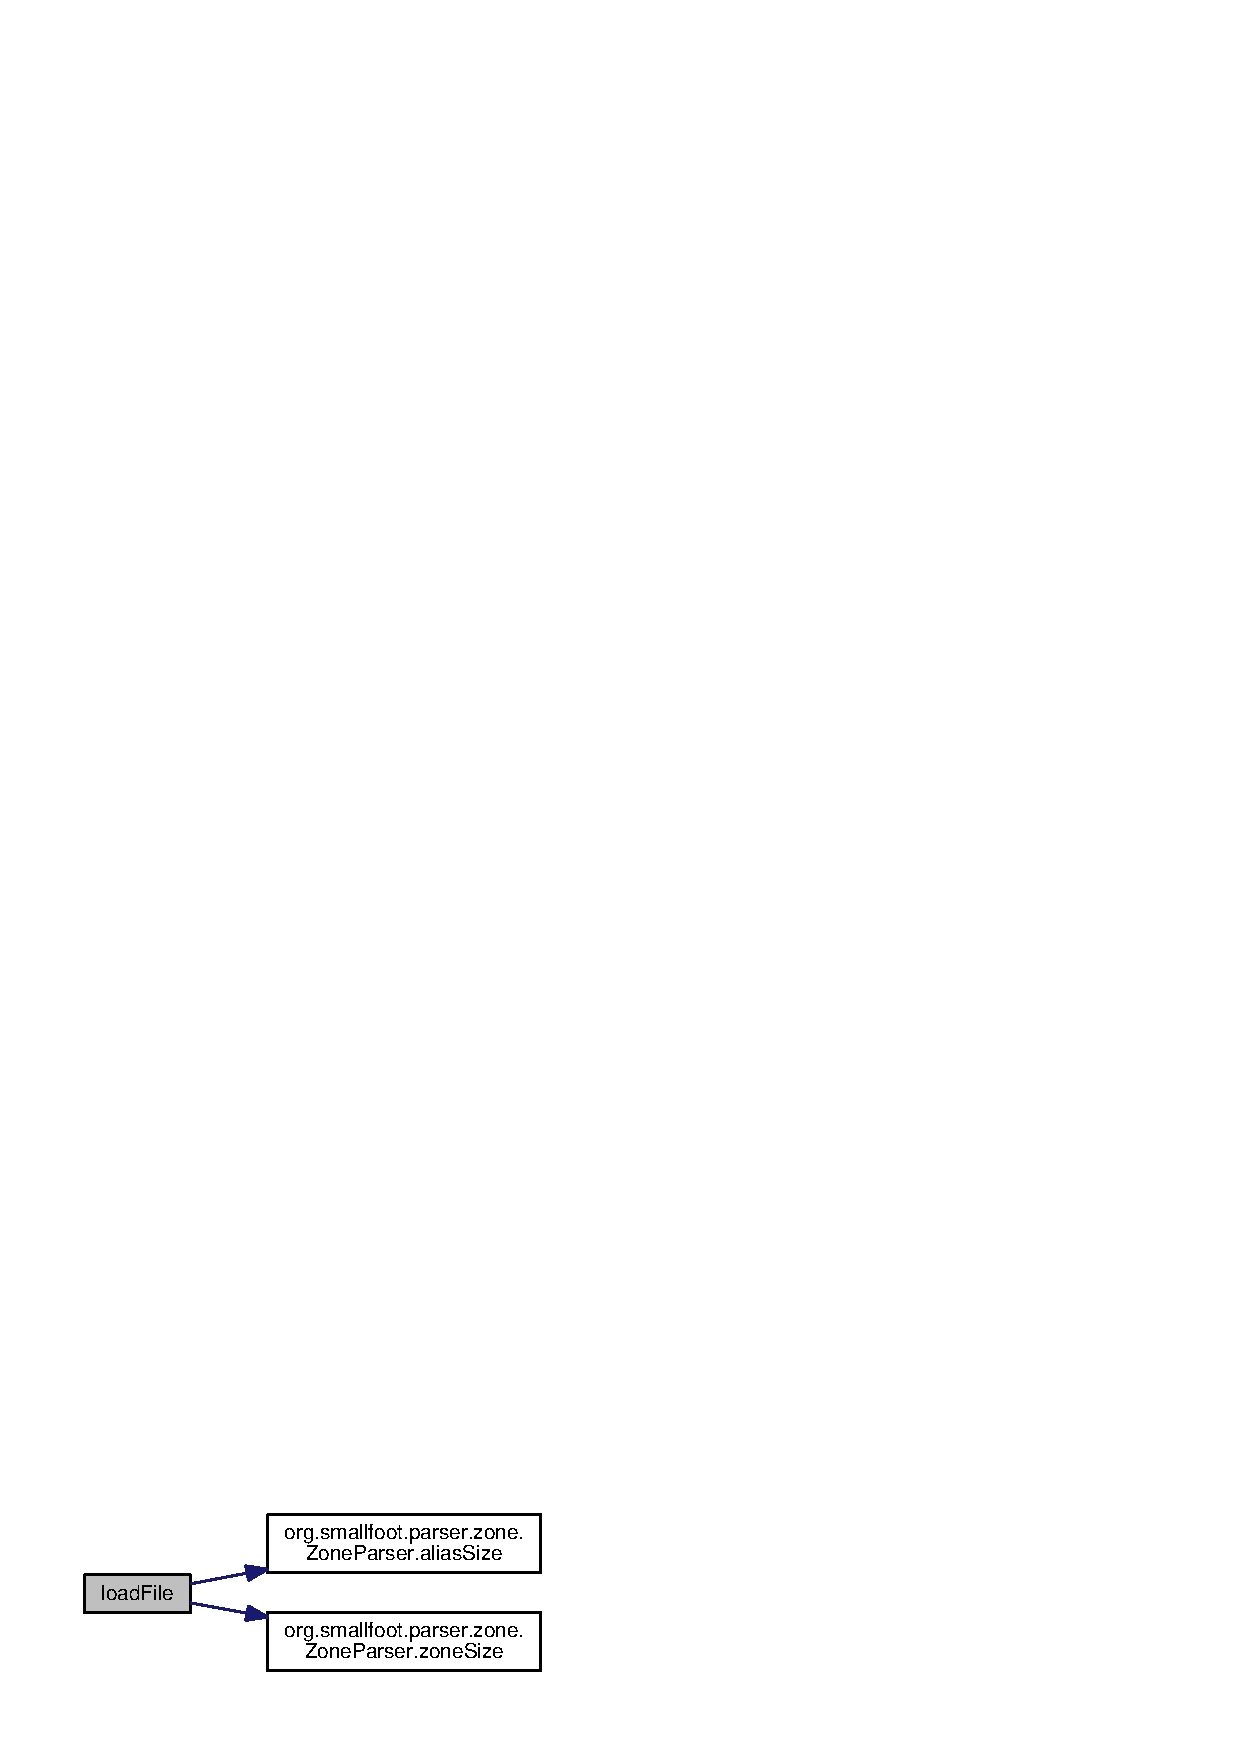
\includegraphics[width=264pt]{classorg_1_1smallfoot_1_1parser_1_1FCParser_a47b0fe73f5a3ae8d0b5e23da3b1b4b63_cgraph}
\end{center}
\end{figure}


\index{org\+::smallfoot\+::parser\+::\+F\+C\+Parser@{org\+::smallfoot\+::parser\+::\+F\+C\+Parser}!main@{main}}
\index{main@{main}!org\+::smallfoot\+::parser\+::\+F\+C\+Parser@{org\+::smallfoot\+::parser\+::\+F\+C\+Parser}}
\subsubsection[{main}]{\setlength{\rightskip}{0pt plus 5cm}static void main (
\begin{DoxyParamCaption}
\item[{String}]{args[$\,$]}
\end{DoxyParamCaption}
)\hspace{0.3cm}{\ttfamily [inline]}, {\ttfamily [static]}}\label{classorg_1_1smallfoot_1_1parser_1_1FCParser_a75988cf84fc6ee7a2ebff36e363021aa}


Main function, as you can tell. 

this function merely parses the command-\/line to dispatch actions to the meat of the meal above. I'm using an actual Get\+Opt because, yes, I'm a U\+N\+I\+X/\+C hack, re-\/using 3-\/decades-\/old knowledge, but this also preserves both extensibility and the ability to use longopts in scripts as a way to self-\/document what the tool's doing.

No real intelligence herein except the parse-\/and-\/redirect action.


\begin{DoxyParams}{Parameters}
{\em args} & as you'd expect, these are commandline arguments given when the jar is activated \\
\hline
\end{DoxyParams}
Always always A\+L\+W\+A\+Y\+S provide a quick reference and a version output

\begin{DoxyRefDesc}{Commandline Options}
\item[{\bf Commandline Options}]-\/\+H$\vert$--help Show a simple help screen as a reminder of options which are understood by the application \end{DoxyRefDesc}
\begin{DoxyRefDesc}{Commandline Options}
\item[{\bf Commandline Options}]
\begin{DoxyCode}
java -jar fcparsers.jar --help 
\end{DoxyCode}
\end{DoxyRefDesc}


\begin{DoxyRefDesc}{Commandline Options}
\item[{\bf Commandline Options}]-\/\+V$\vert$--version Show the current release version for reference \end{DoxyRefDesc}
\begin{DoxyRefDesc}{Commandline Options}
\item[{\bf Commandline Options}]
\begin{DoxyCode}
java -jar fcparsers.jar --version
0.3-151 
\end{DoxyCode}
\end{DoxyRefDesc}


\begin{DoxyRefDesc}{Commandline Options}
\item[{\bf Commandline Options}]-\/\+N$\vert$--nickname=\{file/uri\} Import nicknames by parsing a text stream from various sources \end{DoxyRefDesc}
\begin{DoxyRefDesc}{Commandline Options}
\item[{\bf Commandline Options}]
\begin{DoxyCode}
 java -jar fcparsers.jar --nickname=switch44.zoneshow
Parse results \textcolor{keywordflow}{for} AliShowZoneParser:
Zones: 44
Aliases: 112 (names with one or more WWPNs)
Aliases: 136 (name/WWPN tuples) 
\end{DoxyCode}
 In this example, a zone file was parsed by the Ali\+Show\+Zone\+Parser resulting in 112 nicknames; due to duplicate nicknames, there are actually 136 unique W\+W\+P\+N/alias tuples, which means that (136-\/112) 24 of the W\+W\+P\+Ns have the same alias as other W\+W\+P\+Ns\end{DoxyRefDesc}


\begin{DoxyRefDesc}{Commandline Options}
\item[{\bf Commandline Options}]-\/!$\vert$--check Run an internal check that dependent drivers are available and registered \end{DoxyRefDesc}


Definition at line 296 of file F\+C\+Parser.\+java.



References F\+C\+Parser.\+load\+File(), F\+C\+Parser.\+open\+Source(), F\+C\+Parser.\+register\+Protocols(), and Zone\+Parser.\+summarize().



Here is the call graph for this function\+:\nopagebreak
\begin{figure}[H]
\begin{center}
\leavevmode
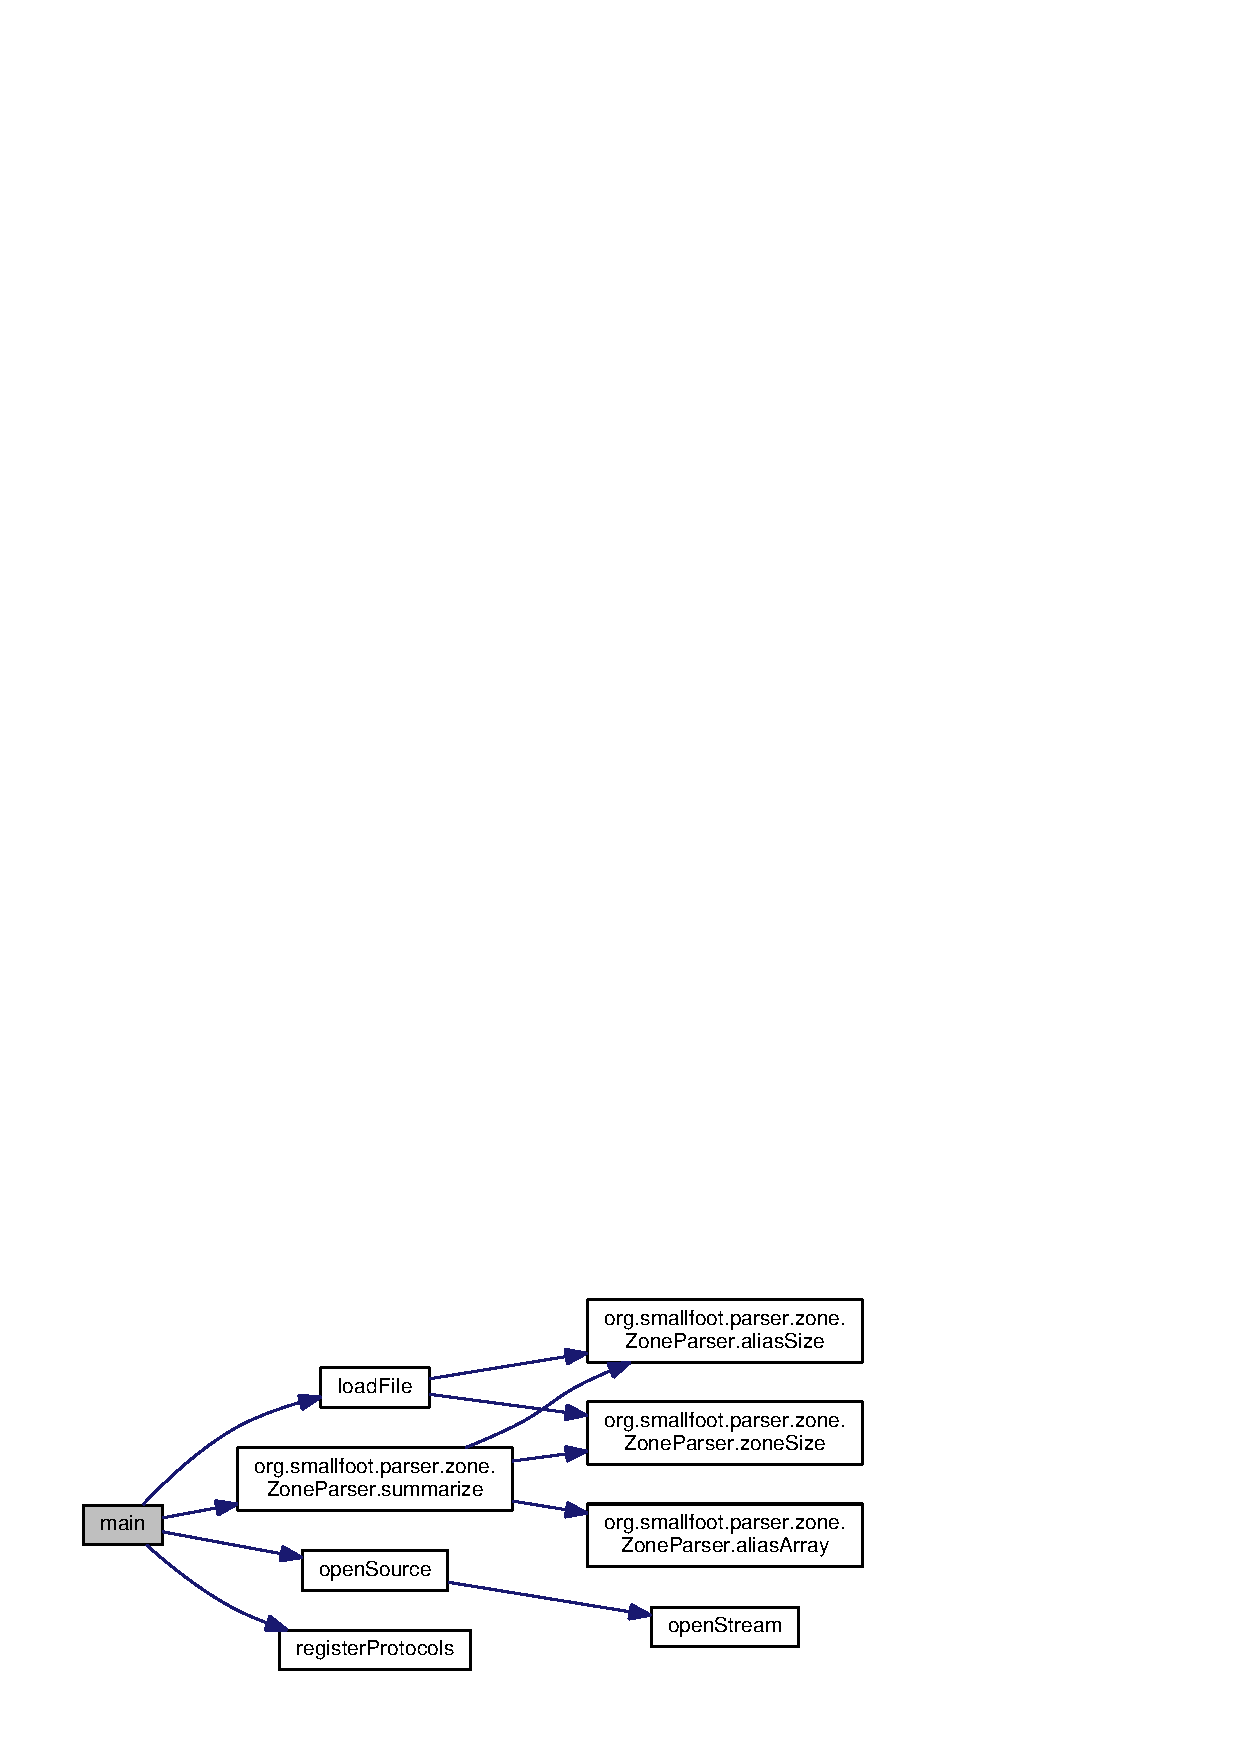
\includegraphics[width=350pt]{classorg_1_1smallfoot_1_1parser_1_1FCParser_a75988cf84fc6ee7a2ebff36e363021aa_cgraph}
\end{center}
\end{figure}


\index{org\+::smallfoot\+::parser\+::\+F\+C\+Parser@{org\+::smallfoot\+::parser\+::\+F\+C\+Parser}!open\+Source@{open\+Source}}
\index{open\+Source@{open\+Source}!org\+::smallfoot\+::parser\+::\+F\+C\+Parser@{org\+::smallfoot\+::parser\+::\+F\+C\+Parser}}
\subsubsection[{open\+Source}]{\setlength{\rightskip}{0pt plus 5cm}static Input\+Stream open\+Source (
\begin{DoxyParamCaption}
\item[{String}]{url, }
\item[{boolean}]{verbose, }
\item[{java.\+util.\+Properties}]{prop}
\end{DoxyParamCaption}
)\hspace{0.3cm}{\ttfamily [inline]}, {\ttfamily [static]}}\label{classorg_1_1smallfoot_1_1parser_1_1FCParser_a6085cf44eb1e750084cff1666eeae8ba}


Create a stream from a U\+R\+L or file name with a convenience workaround for no-\/proto U\+R\+Ls. 

N\+O\+T\+E\+: changes java.\+util.\+Properties

\begin{DoxyReturn}{Returns}
the resulting Input\+Stream 
\end{DoxyReturn}

\begin{DoxyParams}{Parameters}
{\em url} & the resource to open \\
\hline
{\em verbose} & whether to report errors to stdout or run quietly \\
\hline
{\em prop} & Properties through which to pass post-\/\+U\+R\+L options \\
\hline
\end{DoxyParams}


Definition at line 97 of file F\+C\+Parser.\+java.



References F\+C\+Parser.\+open\+Stream().



Referenced by F\+C\+Parser.\+main().



Here is the call graph for this function\+:\nopagebreak
\begin{figure}[H]
\begin{center}
\leavevmode
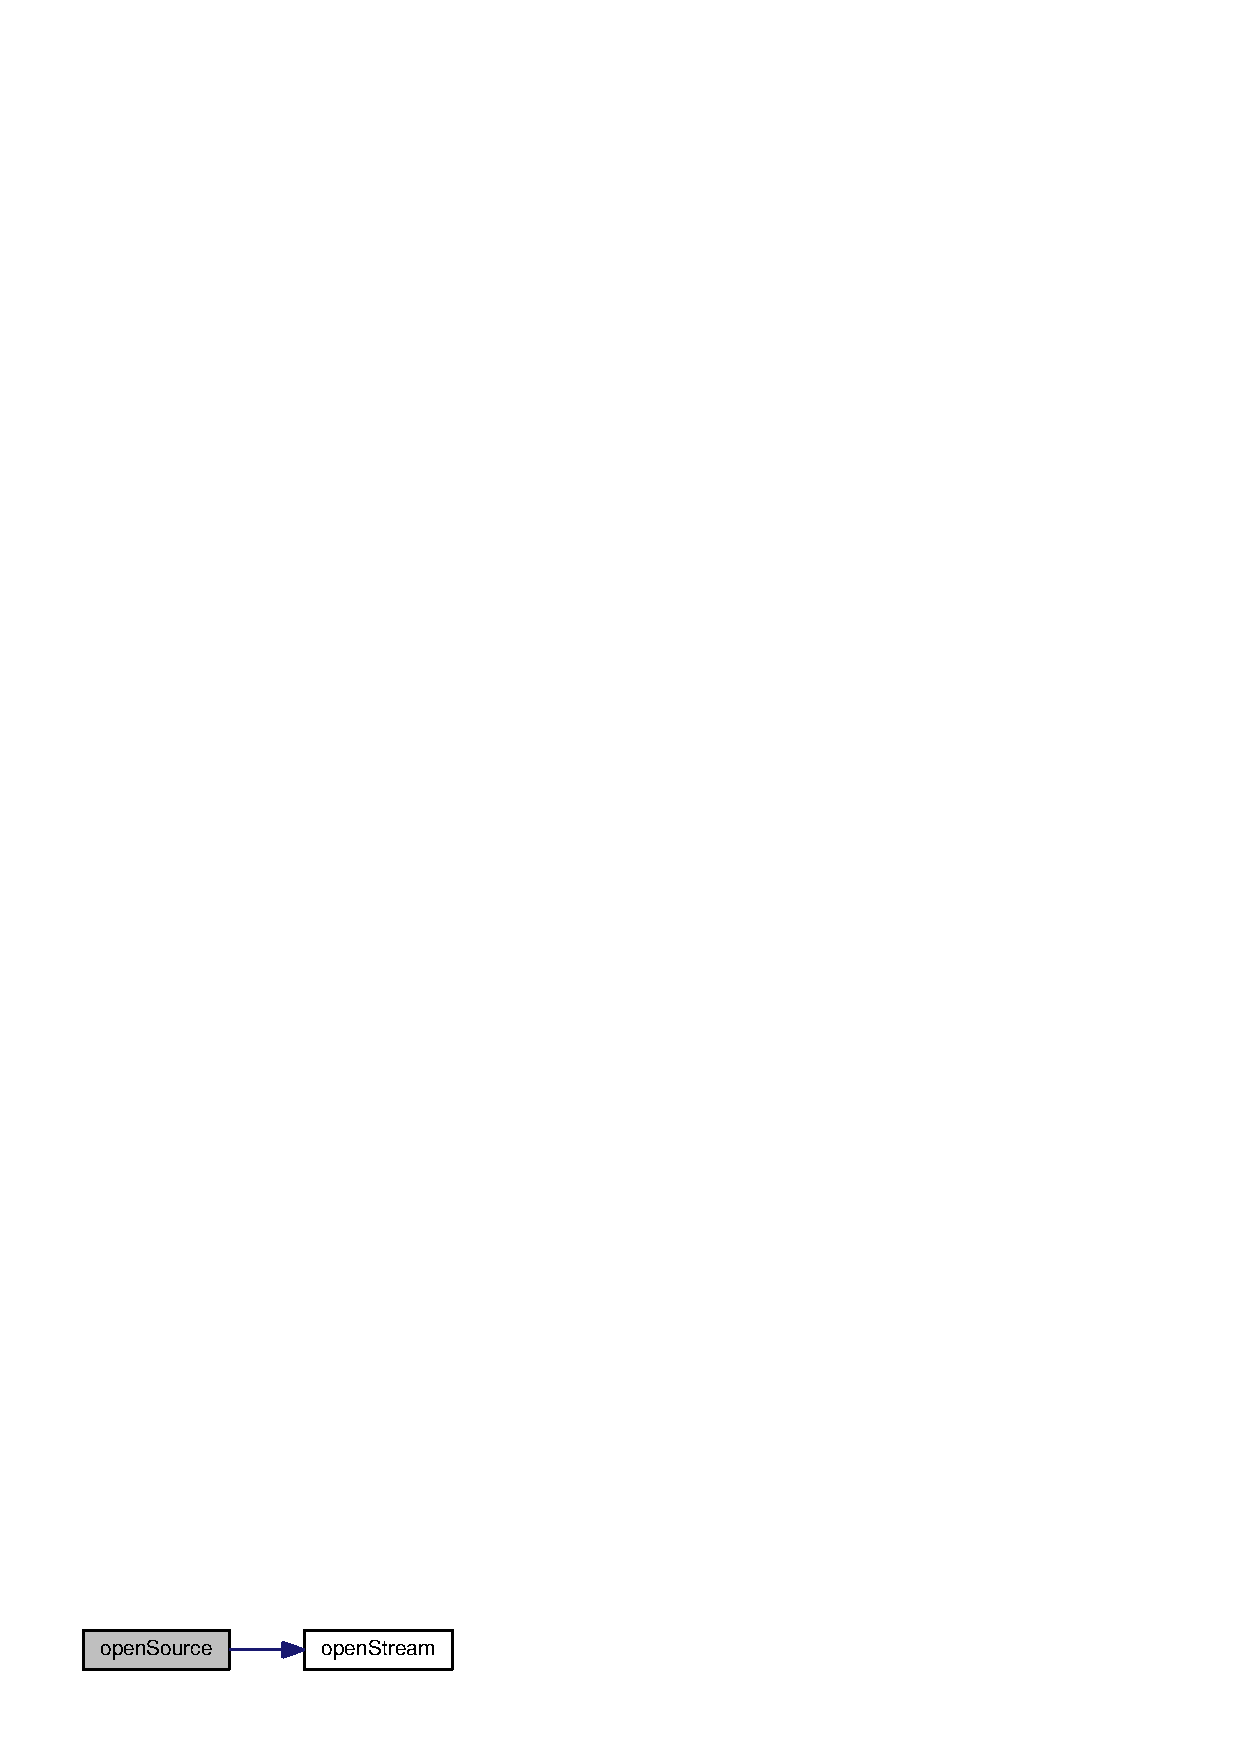
\includegraphics[width=220pt]{classorg_1_1smallfoot_1_1parser_1_1FCParser_a6085cf44eb1e750084cff1666eeae8ba_cgraph}
\end{center}
\end{figure}


\index{org\+::smallfoot\+::parser\+::\+F\+C\+Parser@{org\+::smallfoot\+::parser\+::\+F\+C\+Parser}!open\+Stream@{open\+Stream}}
\index{open\+Stream@{open\+Stream}!org\+::smallfoot\+::parser\+::\+F\+C\+Parser@{org\+::smallfoot\+::parser\+::\+F\+C\+Parser}}
\subsubsection[{open\+Stream}]{\setlength{\rightskip}{0pt plus 5cm}static java.\+io.\+Input\+Stream open\+Stream (
\begin{DoxyParamCaption}
\item[{String}]{uri}
\end{DoxyParamCaption}
) throws java.\+io.\+File\+Not\+Found\+Exception, java.\+net.\+Malformed\+U\+R\+L\+Exception, java.\+io.\+I\+O\+Exception\hspace{0.3cm}{\ttfamily [inline]}, {\ttfamily [static]}}\label{classorg_1_1smallfoot_1_1parser_1_1FCParser_a87eb2ebceee6e66dc59ed239d2220a56}


Produce an Input\+Stream for the given uri in a way that corresponds to the url protocol. 

\begin{DoxyReturn}{Returns}
Input\+Stream ready to offer back the data 
\end{DoxyReturn}

\begin{DoxyParams}{Parameters}
{\em uri} & the {\tt file\+://} resource of a file, ie \char`\"{}file\+:///sample.\+csv\char`\"{} \\
\hline
\end{DoxyParams}


Definition at line 37 of file F\+C\+Parser.\+java.



Referenced by F\+C\+Parser.\+open\+Source().

\index{org\+::smallfoot\+::parser\+::\+F\+C\+Parser@{org\+::smallfoot\+::parser\+::\+F\+C\+Parser}!register\+Protocols@{register\+Protocols}}
\index{register\+Protocols@{register\+Protocols}!org\+::smallfoot\+::parser\+::\+F\+C\+Parser@{org\+::smallfoot\+::parser\+::\+F\+C\+Parser}}
\subsubsection[{register\+Protocols}]{\setlength{\rightskip}{0pt plus 5cm}static void register\+Protocols (
\begin{DoxyParamCaption}
{}
\end{DoxyParamCaption}
)\hspace{0.3cm}{\ttfamily [inline]}, {\ttfamily [static]}}\label{classorg_1_1smallfoot_1_1parser_1_1FCParser_a9f16799674af7de1e539f0b54dbea72a}


Collect in a single place the process to register protocol handlers. 

This function checks for current protocol handlers and adds the ones we bring to that list. If no \char`\"{}java.\+protocol.\+handler.\+pkgs\char`\"{} exists, we simply provide one. System Properties are overwritten in this process.

as the number of handlers increases, we can make corresponding changes herein without consuming projects having to know or care about this.

The format of \char`\"{}java.\+protocol.\+handler.\+pkgs\char`\"{} is typically described in java.\+net.\+U\+R\+L(\+String,\+String,int,\+String) \begin{DoxySeeAlso}{See also}
java.\+lang.\+System.\+set\+Property(\+String,\+String) 
\end{DoxySeeAlso}


Definition at line 66 of file F\+C\+Parser.\+java.



Referenced by F\+C\+Parser.\+main().



The documentation for this class was generated from the following file\+:\begin{DoxyCompactItemize}
\item 
java/{\bf F\+C\+Parser.\+java}\end{DoxyCompactItemize}

\section{Handler Class Reference}
\label{classorg_1_1smallfoot_1_1parser_1_1osmsql_1_1Handler}\index{Handler@{Handler}}


Inheritance diagram for Handler\+:\nopagebreak
\begin{figure}[H]
\begin{center}
\leavevmode
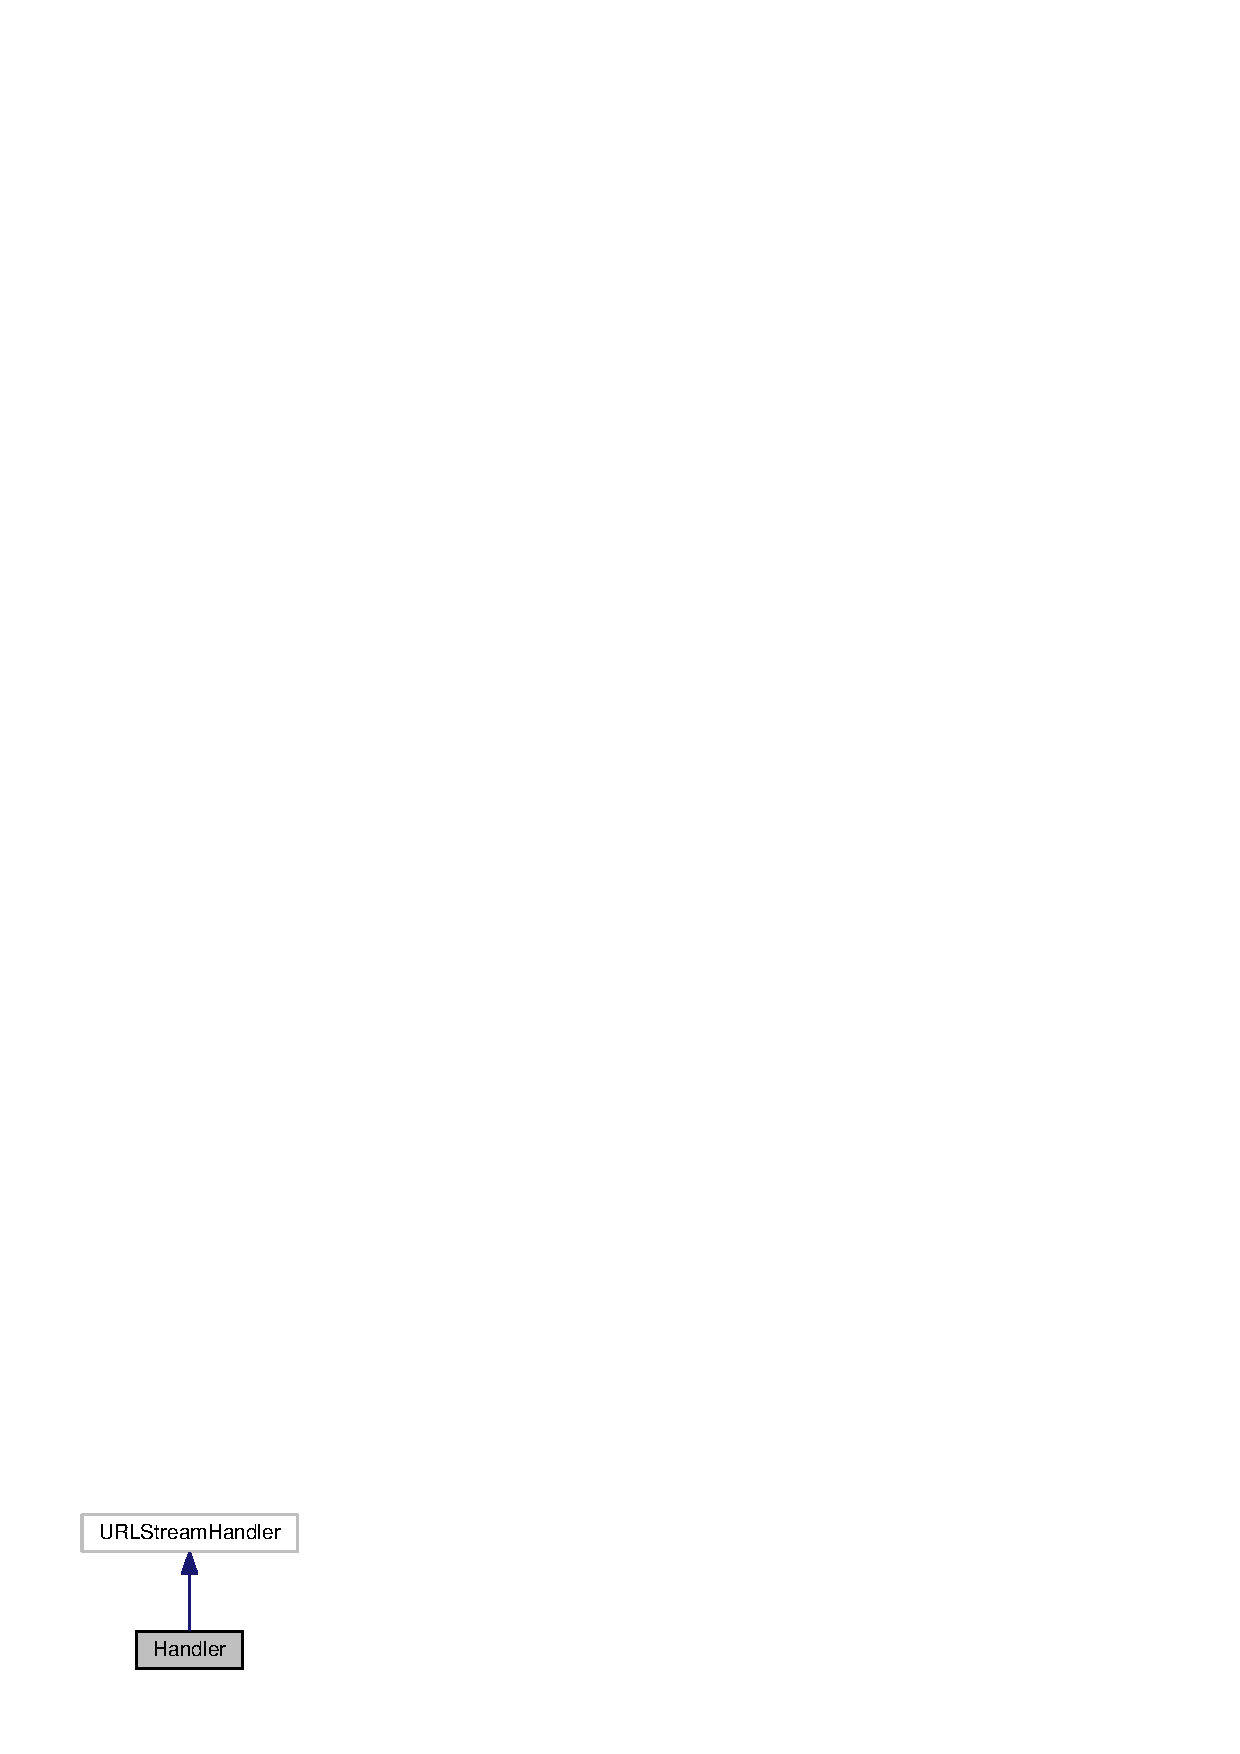
\includegraphics[width=146pt]{classorg_1_1smallfoot_1_1parser_1_1osmsql_1_1Handler__inherit__graph}
\end{center}
\end{figure}


Collaboration diagram for Handler\+:\nopagebreak
\begin{figure}[H]
\begin{center}
\leavevmode
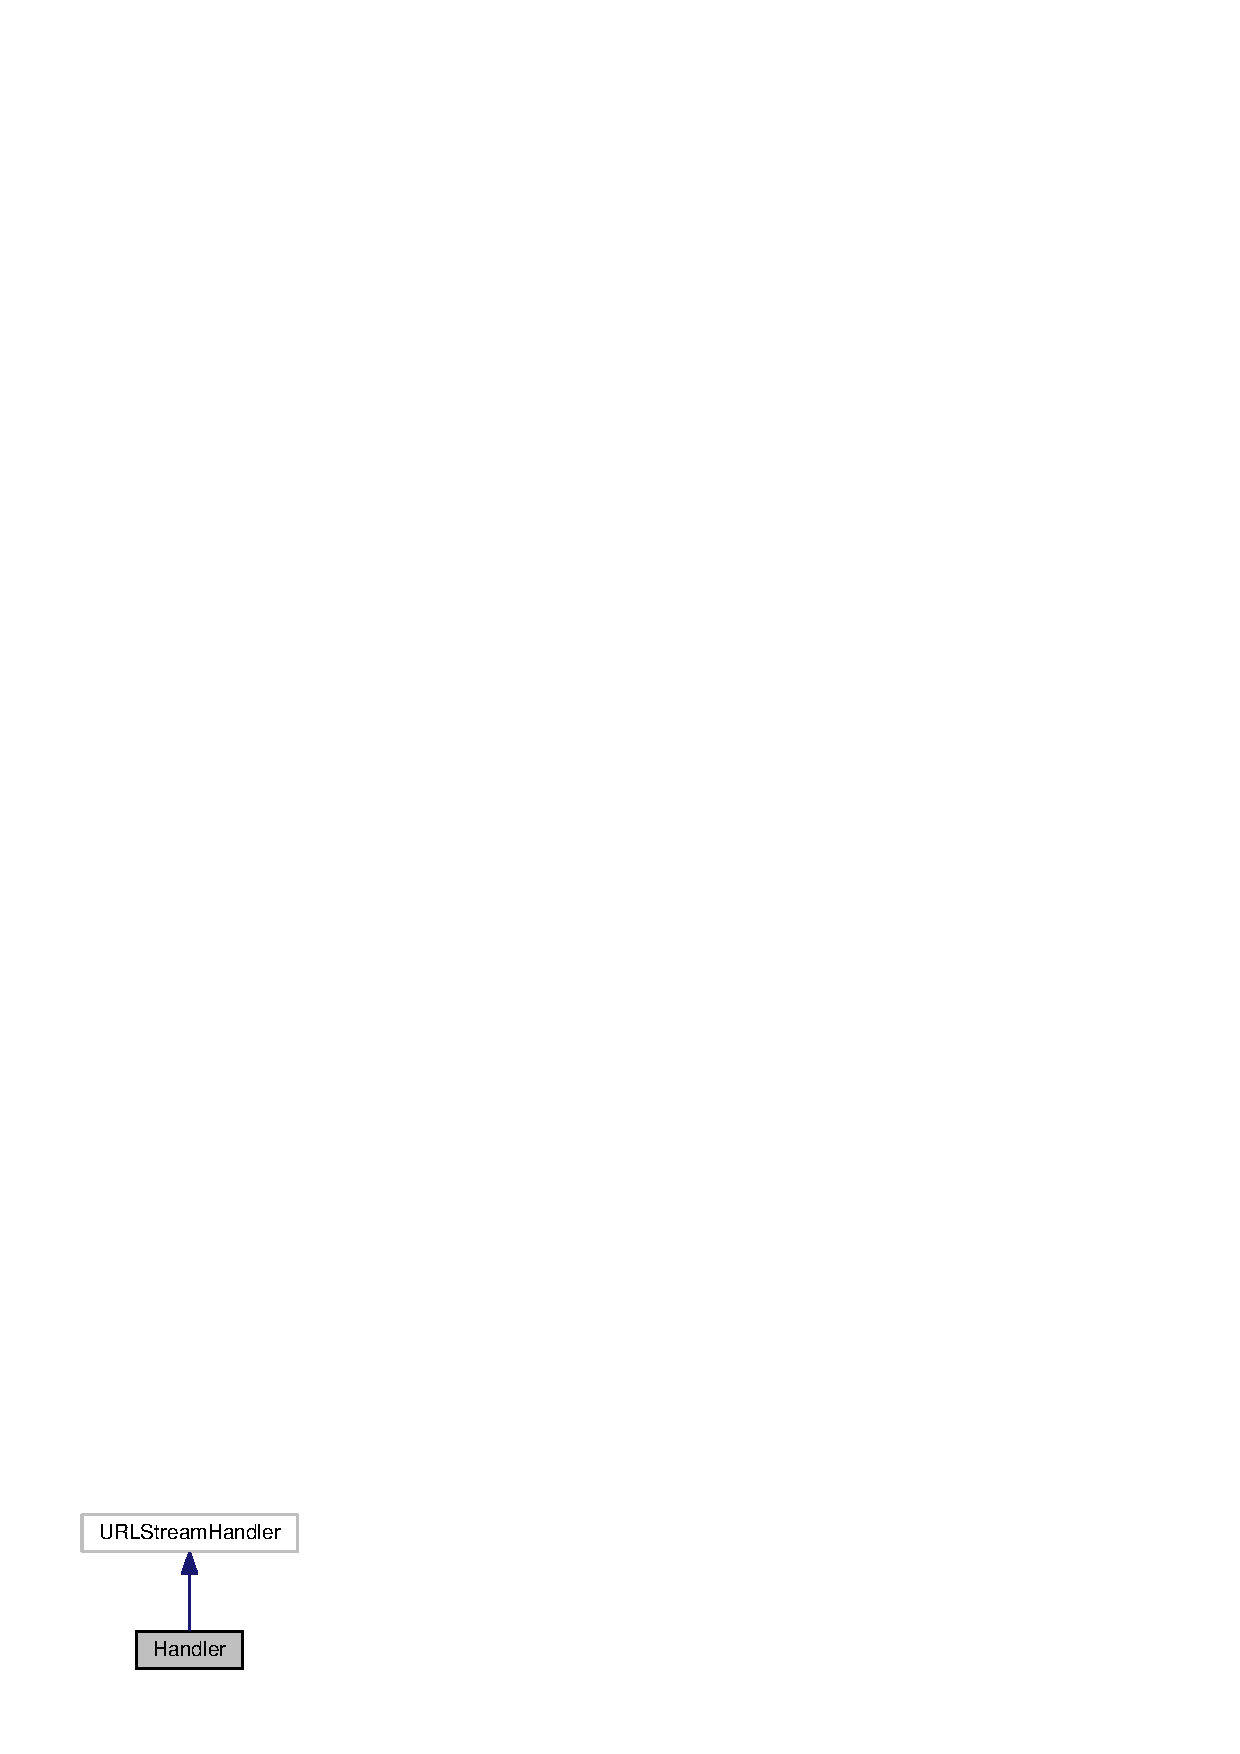
\includegraphics[width=146pt]{classorg_1_1smallfoot_1_1parser_1_1osmsql_1_1Handler__coll__graph}
\end{center}
\end{figure}
\subsection*{Protected Member Functions}
\begin{DoxyCompactItemize}
\item 
U\+R\+L\+Connection {\bf open\+Connection} (U\+R\+L url)
\begin{DoxyCompactList}\small\item\em \doxyref{open\+Connection(\+U\+R\+L)}{p.}{classorg_1_1smallfoot_1_1parser_1_1osmsql_1_1Handler_a3838795af42df5d7757e609b8b312956} overrides java.\+net.\+U\+R\+L\+Stream\+Handler.\+open\+Connection(\+U\+R\+L) by wrapping a proper connection with prototype-\/matching call and parameters \end{DoxyCompactList}\end{DoxyCompactItemize}


\subsection{Detailed Description}


Definition at line 21 of file Handler.\+java.



\subsection{Member Function Documentation}
\index{org\+::smallfoot\+::parser\+::osmsql\+::\+Handler@{org\+::smallfoot\+::parser\+::osmsql\+::\+Handler}!open\+Connection@{open\+Connection}}
\index{open\+Connection@{open\+Connection}!org\+::smallfoot\+::parser\+::osmsql\+::\+Handler@{org\+::smallfoot\+::parser\+::osmsql\+::\+Handler}}
\subsubsection[{open\+Connection}]{\setlength{\rightskip}{0pt plus 5cm}U\+R\+L\+Connection open\+Connection (
\begin{DoxyParamCaption}
\item[{U\+R\+L}]{url}
\end{DoxyParamCaption}
)\hspace{0.3cm}{\ttfamily [inline]}, {\ttfamily [protected]}}\label{classorg_1_1smallfoot_1_1parser_1_1osmsql_1_1Handler_a3838795af42df5d7757e609b8b312956}


\doxyref{open\+Connection(\+U\+R\+L)}{p.}{classorg_1_1smallfoot_1_1parser_1_1osmsql_1_1Handler_a3838795af42df5d7757e609b8b312956} overrides java.\+net.\+U\+R\+L\+Stream\+Handler.\+open\+Connection(\+U\+R\+L) by wrapping a proper connection with prototype-\/matching call and parameters 

\begin{DoxyReturn}{Returns}
populated connection as \doxyref{org.\+smallfoot.\+parser.\+osmsql.\+O\+S\+M\+U\+R\+L\+Connection(\+Connection)}{p.}{classorg_1_1smallfoot_1_1parser_1_1osmsql_1_1OSMURLConnection} 
\end{DoxyReturn}

\begin{DoxyParams}{Parameters}
{\em url} & U\+R\+L to which we need to connect \\
\hline
\end{DoxyParams}


Definition at line 29 of file Handler.\+java.



The documentation for this class was generated from the following file\+:\begin{DoxyCompactItemize}
\item 
java/genproto/osmsql/{\bf Handler.\+java}\end{DoxyCompactItemize}

\section{Handler Class Reference}
\label{classorg_1_1smallfoot_1_1parser_1_1bna_1_1Handler}\index{Handler@{Handler}}


Inheritance diagram for Handler\+:
\nopagebreak
\begin{figure}[H]
\begin{center}
\leavevmode
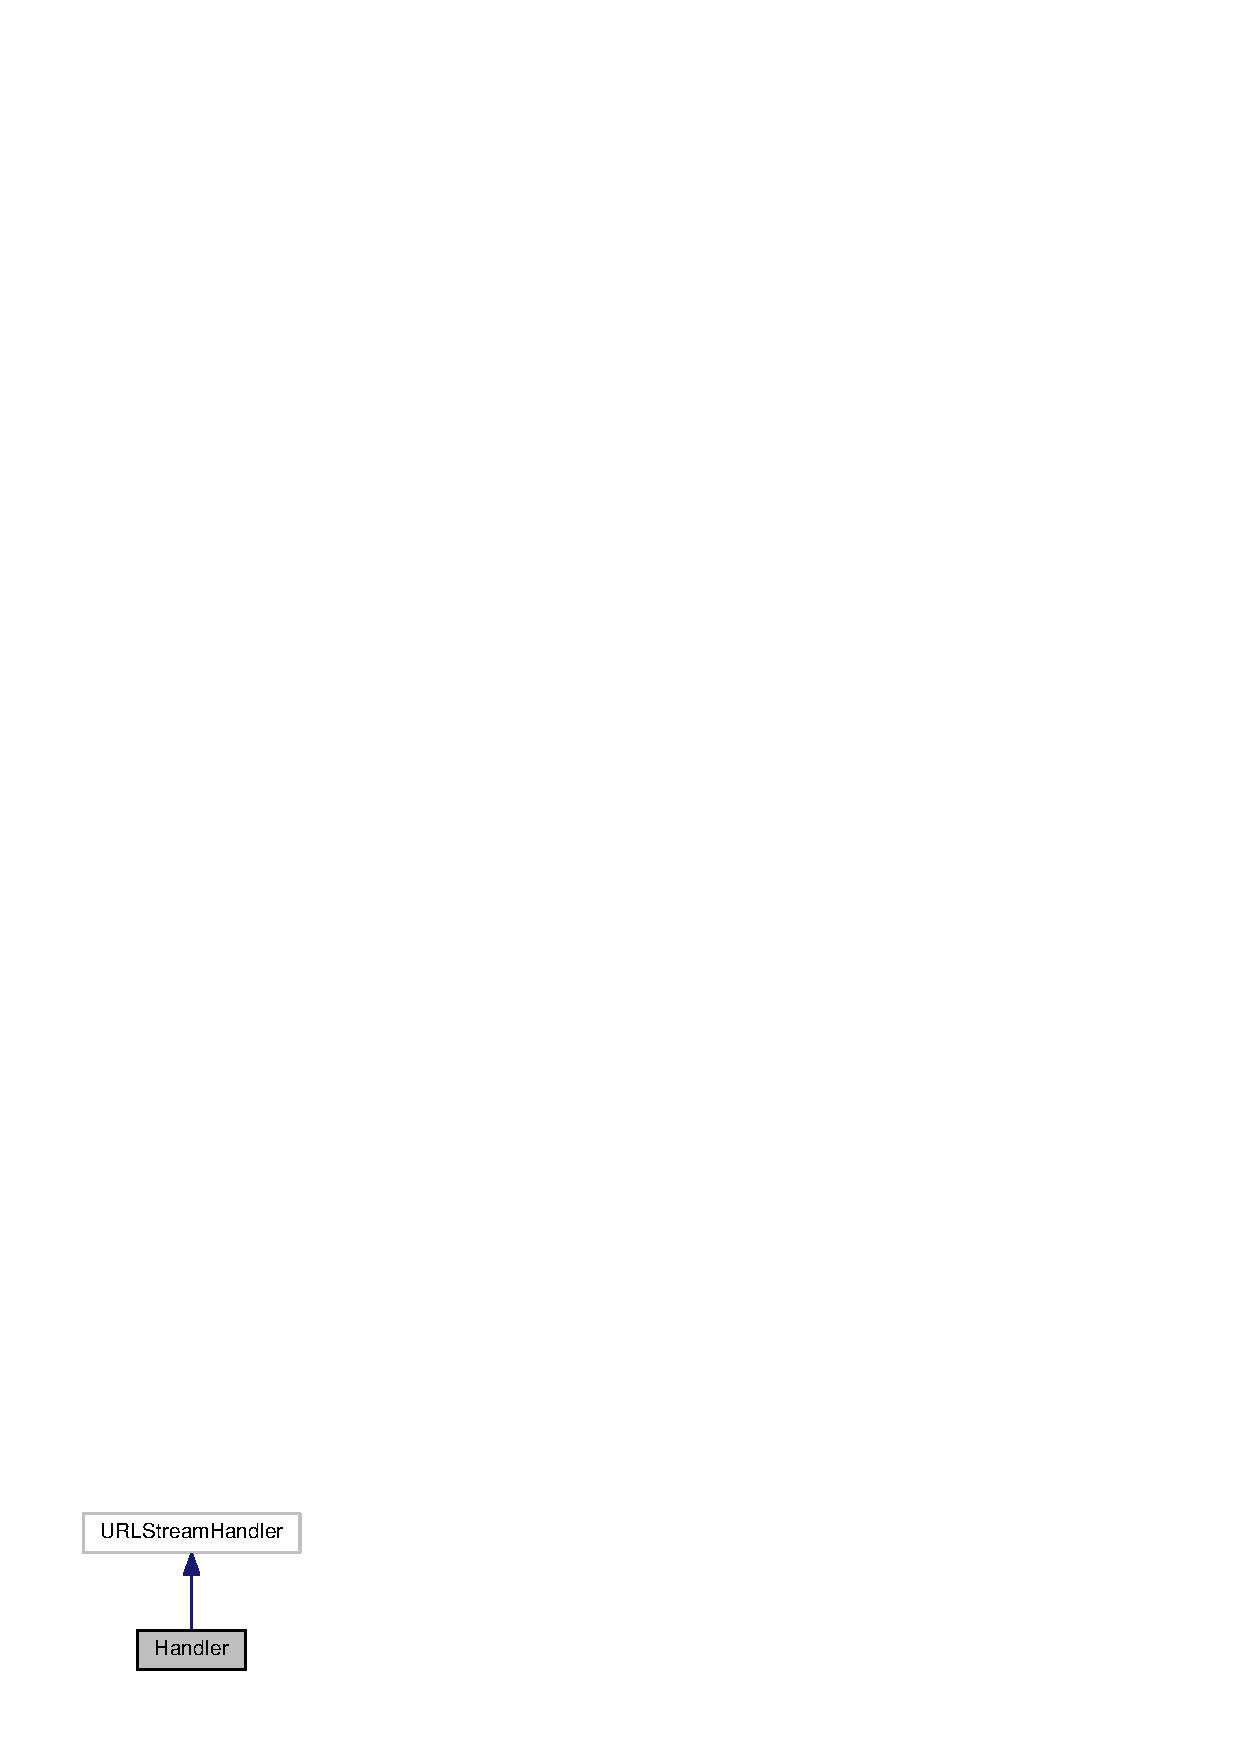
\includegraphics[width=146pt]{classorg_1_1smallfoot_1_1parser_1_1bna_1_1Handler__inherit__graph}
\end{center}
\end{figure}


Collaboration diagram for Handler\+:
\nopagebreak
\begin{figure}[H]
\begin{center}
\leavevmode
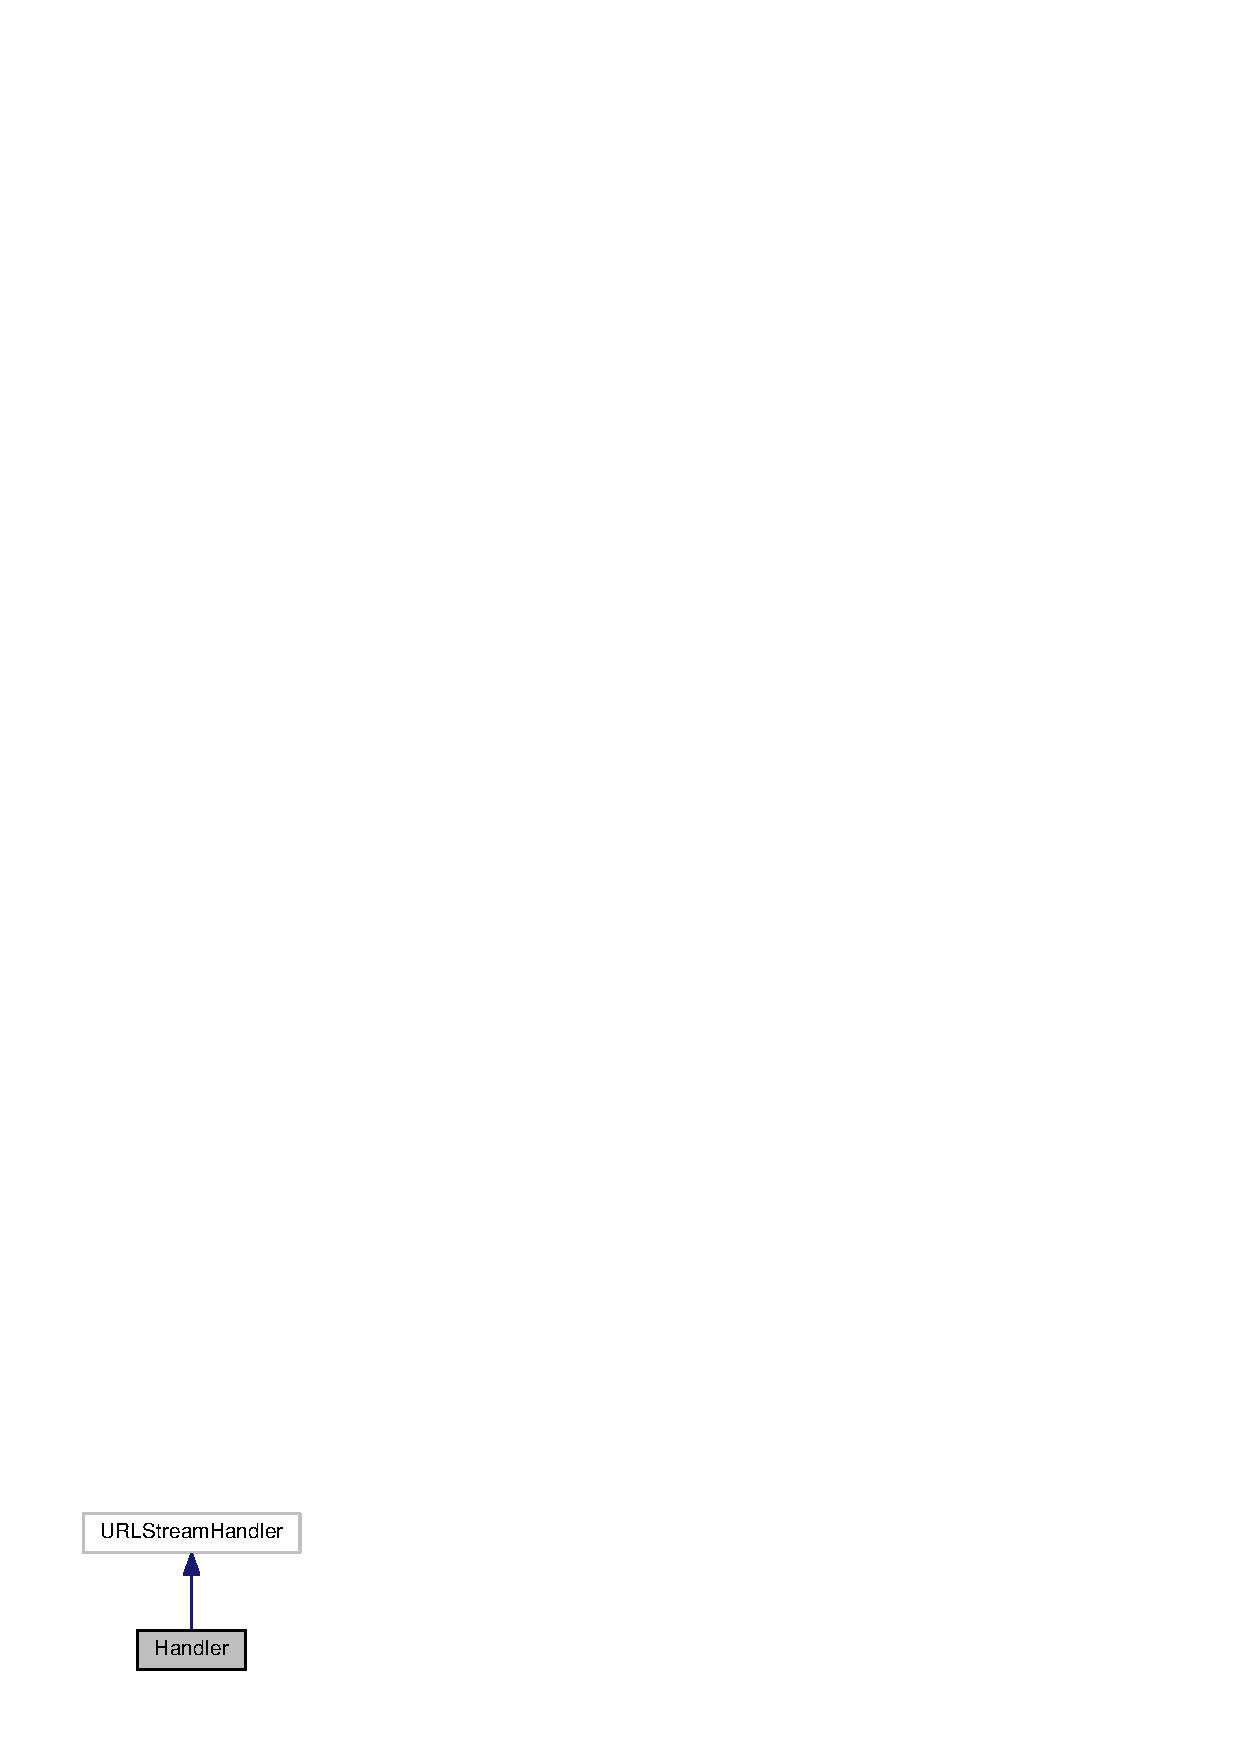
\includegraphics[width=146pt]{classorg_1_1smallfoot_1_1parser_1_1bna_1_1Handler__coll__graph}
\end{center}
\end{figure}
\subsection*{Protected Member Functions}
\begin{DoxyCompactItemize}
\item 
U\+R\+L\+Connection {\bf open\+Connection} (U\+R\+L url)
\begin{DoxyCompactList}\small\item\em \doxyref{open\+Connection(\+U\+R\+L)}{p.}{classorg_1_1smallfoot_1_1parser_1_1bna_1_1Handler_a3838795af42df5d7757e609b8b312956} overrides java.\+net.\+U\+R\+L\+Stream\+Handler.\+open\+Connection(\+U\+R\+L) by wrapping a proper connection with prototype-\/matching call and parameters \end{DoxyCompactList}\end{DoxyCompactItemize}


\subsection{Detailed Description}


Definition at line 21 of file Handler.\+java.



\subsection{Member Function Documentation}
\index{org\+::smallfoot\+::parser\+::bna\+::\+Handler@{org\+::smallfoot\+::parser\+::bna\+::\+Handler}!open\+Connection@{open\+Connection}}
\index{open\+Connection@{open\+Connection}!org\+::smallfoot\+::parser\+::bna\+::\+Handler@{org\+::smallfoot\+::parser\+::bna\+::\+Handler}}
\subsubsection[{open\+Connection}]{\setlength{\rightskip}{0pt plus 5cm}U\+R\+L\+Connection open\+Connection (
\begin{DoxyParamCaption}
\item[{U\+R\+L}]{url}
\end{DoxyParamCaption}
)\hspace{0.3cm}{\ttfamily [inline]}, {\ttfamily [protected]}}\label{classorg_1_1smallfoot_1_1parser_1_1bna_1_1Handler_a3838795af42df5d7757e609b8b312956}


\doxyref{open\+Connection(\+U\+R\+L)}{p.}{classorg_1_1smallfoot_1_1parser_1_1bna_1_1Handler_a3838795af42df5d7757e609b8b312956} overrides java.\+net.\+U\+R\+L\+Stream\+Handler.\+open\+Connection(\+U\+R\+L) by wrapping a proper connection with prototype-\/matching call and parameters 

\begin{DoxyReturn}{Returns}
populated connection as \doxyref{org.\+smallfoot.\+parser.\+bnapsql.\+B\+N\+A\+P\+U\+R\+L\+Connection(\+Connection)}{p.}{classorg_1_1smallfoot_1_1parser_1_1bnapsql_1_1BNAPURLConnection} 
\end{DoxyReturn}

\begin{DoxyParams}{Parameters}
{\em url} & U\+R\+L to which we need to connect \\
\hline
\end{DoxyParams}


Definition at line 29 of file Handler.\+java.



The documentation for this class was generated from the following file\+:\begin{DoxyCompactItemize}
\item 
java/genproto/bna/{\bf Handler.\+java}\end{DoxyCompactItemize}

\section{Handler Class Reference}
\label{classorg_1_1smallfoot_1_1parser_1_1cmcne_1_1Handler}\index{Handler@{Handler}}


Inheritance diagram for Handler\+:\nopagebreak
\begin{figure}[H]
\begin{center}
\leavevmode
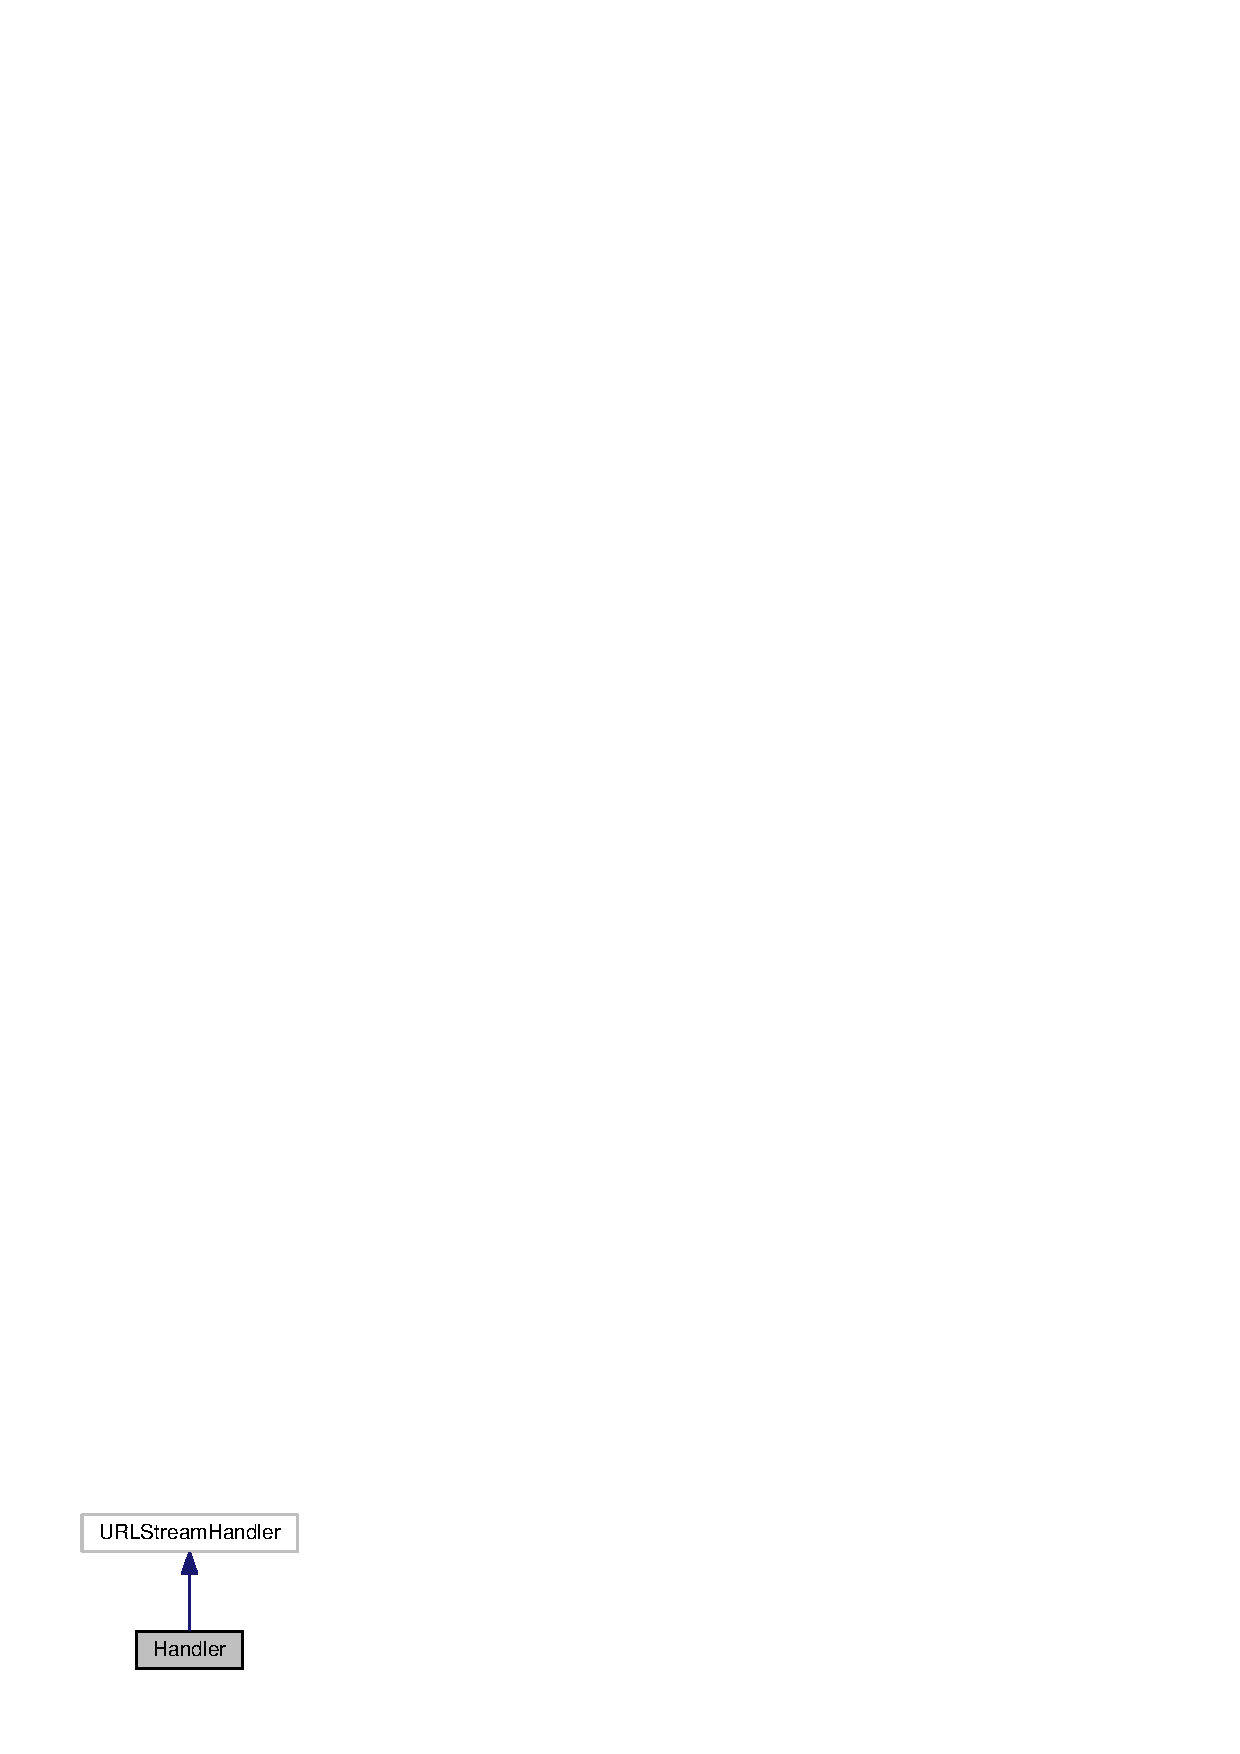
\includegraphics[width=146pt]{classorg_1_1smallfoot_1_1parser_1_1cmcne_1_1Handler__inherit__graph}
\end{center}
\end{figure}


Collaboration diagram for Handler\+:\nopagebreak
\begin{figure}[H]
\begin{center}
\leavevmode
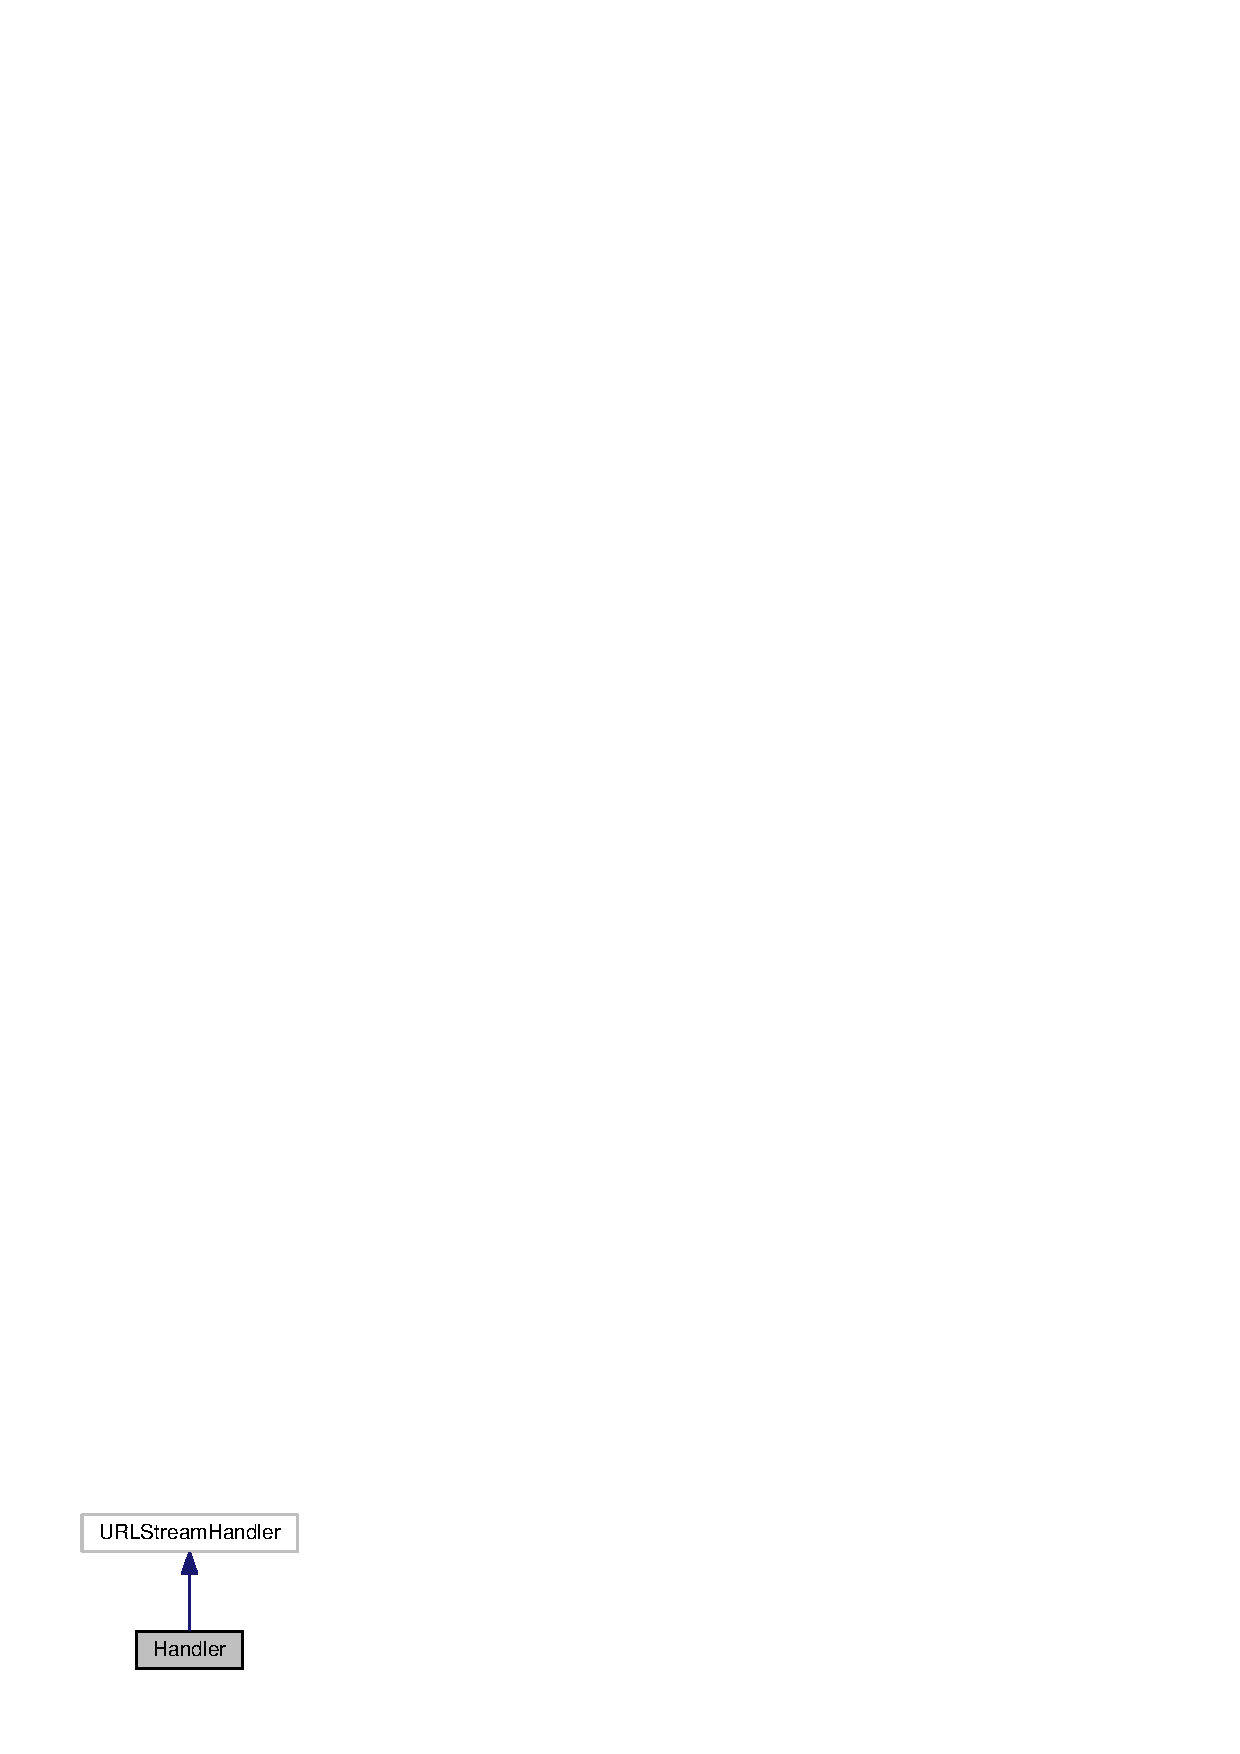
\includegraphics[width=146pt]{classorg_1_1smallfoot_1_1parser_1_1cmcne_1_1Handler__coll__graph}
\end{center}
\end{figure}
\subsection*{Protected Member Functions}
\begin{DoxyCompactItemize}
\item 
U\+R\+L\+Connection {\bf open\+Connection} (U\+R\+L url)
\begin{DoxyCompactList}\small\item\em \doxyref{open\+Connection(\+U\+R\+L)}{p.}{classorg_1_1smallfoot_1_1parser_1_1cmcne_1_1Handler_a3838795af42df5d7757e609b8b312956} overrides java.\+net.\+U\+R\+L\+Stream\+Handler.\+open\+Connection(\+U\+R\+L) by wrapping a proper connection with prototype-\/matching call and parameters \end{DoxyCompactList}\item 
int {\bf get\+Default\+Port} ()
\end{DoxyCompactItemize}


\subsection{Detailed Description}


Definition at line 21 of file Handler.\+java.



\subsection{Member Function Documentation}
\index{org\+::smallfoot\+::parser\+::cmcne\+::\+Handler@{org\+::smallfoot\+::parser\+::cmcne\+::\+Handler}!get\+Default\+Port@{get\+Default\+Port}}
\index{get\+Default\+Port@{get\+Default\+Port}!org\+::smallfoot\+::parser\+::cmcne\+::\+Handler@{org\+::smallfoot\+::parser\+::cmcne\+::\+Handler}}
\subsubsection[{get\+Default\+Port}]{\setlength{\rightskip}{0pt plus 5cm}int get\+Default\+Port (
\begin{DoxyParamCaption}
{}
\end{DoxyParamCaption}
)\hspace{0.3cm}{\ttfamily [inline]}, {\ttfamily [protected]}}\label{classorg_1_1smallfoot_1_1parser_1_1cmcne_1_1Handler_aadc354b6a8746020e9961fbcb433427c}


Definition at line 34 of file Handler.\+java.

\index{org\+::smallfoot\+::parser\+::cmcne\+::\+Handler@{org\+::smallfoot\+::parser\+::cmcne\+::\+Handler}!open\+Connection@{open\+Connection}}
\index{open\+Connection@{open\+Connection}!org\+::smallfoot\+::parser\+::cmcne\+::\+Handler@{org\+::smallfoot\+::parser\+::cmcne\+::\+Handler}}
\subsubsection[{open\+Connection}]{\setlength{\rightskip}{0pt plus 5cm}U\+R\+L\+Connection open\+Connection (
\begin{DoxyParamCaption}
\item[{U\+R\+L}]{url}
\end{DoxyParamCaption}
)\hspace{0.3cm}{\ttfamily [inline]}, {\ttfamily [protected]}}\label{classorg_1_1smallfoot_1_1parser_1_1cmcne_1_1Handler_a3838795af42df5d7757e609b8b312956}


\doxyref{open\+Connection(\+U\+R\+L)}{p.}{classorg_1_1smallfoot_1_1parser_1_1cmcne_1_1Handler_a3838795af42df5d7757e609b8b312956} overrides java.\+net.\+U\+R\+L\+Stream\+Handler.\+open\+Connection(\+U\+R\+L) by wrapping a proper connection with prototype-\/matching call and parameters 

\begin{DoxyReturn}{Returns}
populated connection as \doxyref{org.\+smallfoot.\+parser.\+bnapsql.\+B\+N\+A\+P\+U\+R\+L\+Connection(\+Connection)}{p.}{classorg_1_1smallfoot_1_1parser_1_1bnapsql_1_1BNAPURLConnection} 
\end{DoxyReturn}

\begin{DoxyParams}{Parameters}
{\em url} & U\+R\+L to which we need to connect \\
\hline
\end{DoxyParams}


Definition at line 29 of file Handler.\+java.



The documentation for this class was generated from the following file\+:\begin{DoxyCompactItemize}
\item 
java/genproto/cmcne/{\bf Handler.\+java}\end{DoxyCompactItemize}

\section{Handler Class Reference}
\label{classorg_1_1smallfoot_1_1parser_1_1dcfm_1_1Handler}\index{Handler@{Handler}}


Inheritance diagram for Handler\+:\nopagebreak
\begin{figure}[H]
\begin{center}
\leavevmode
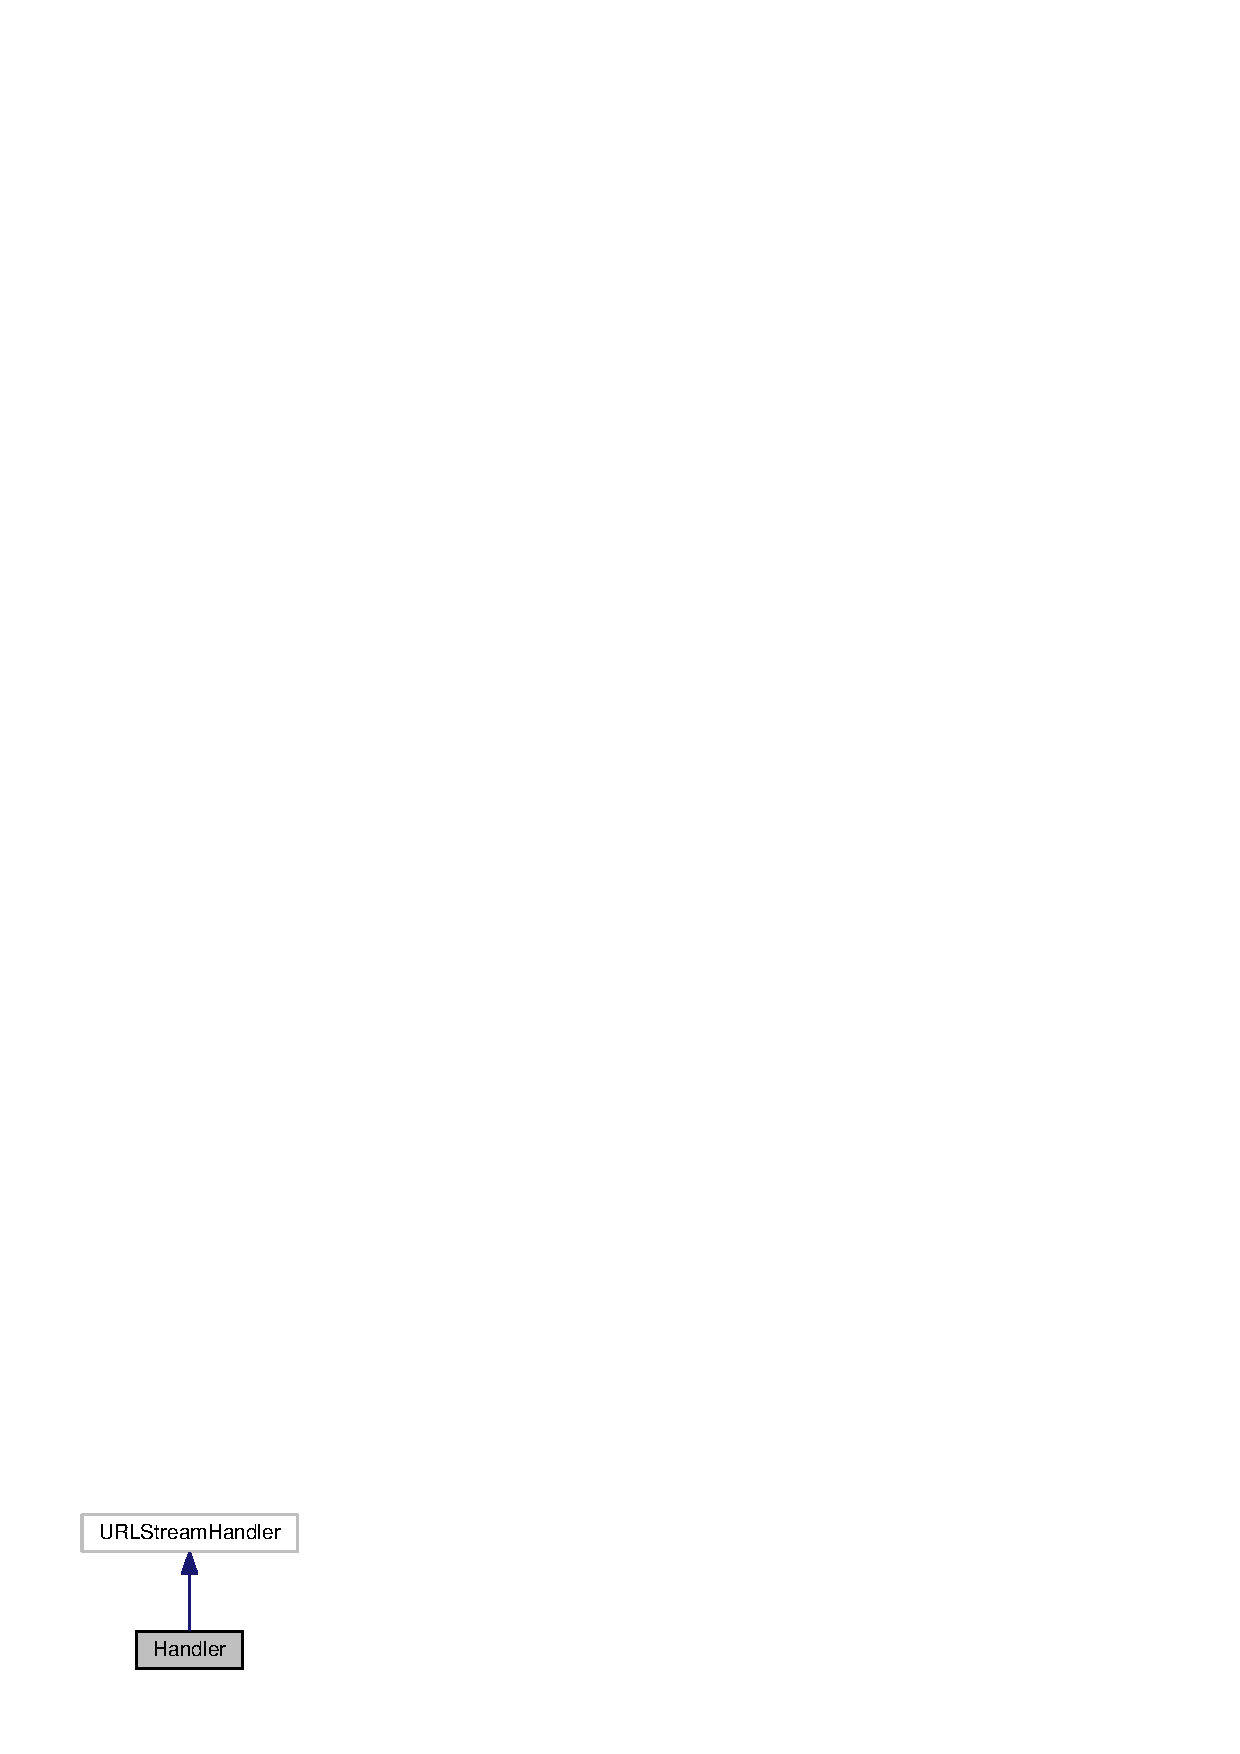
\includegraphics[width=146pt]{classorg_1_1smallfoot_1_1parser_1_1dcfm_1_1Handler__inherit__graph}
\end{center}
\end{figure}


Collaboration diagram for Handler\+:\nopagebreak
\begin{figure}[H]
\begin{center}
\leavevmode
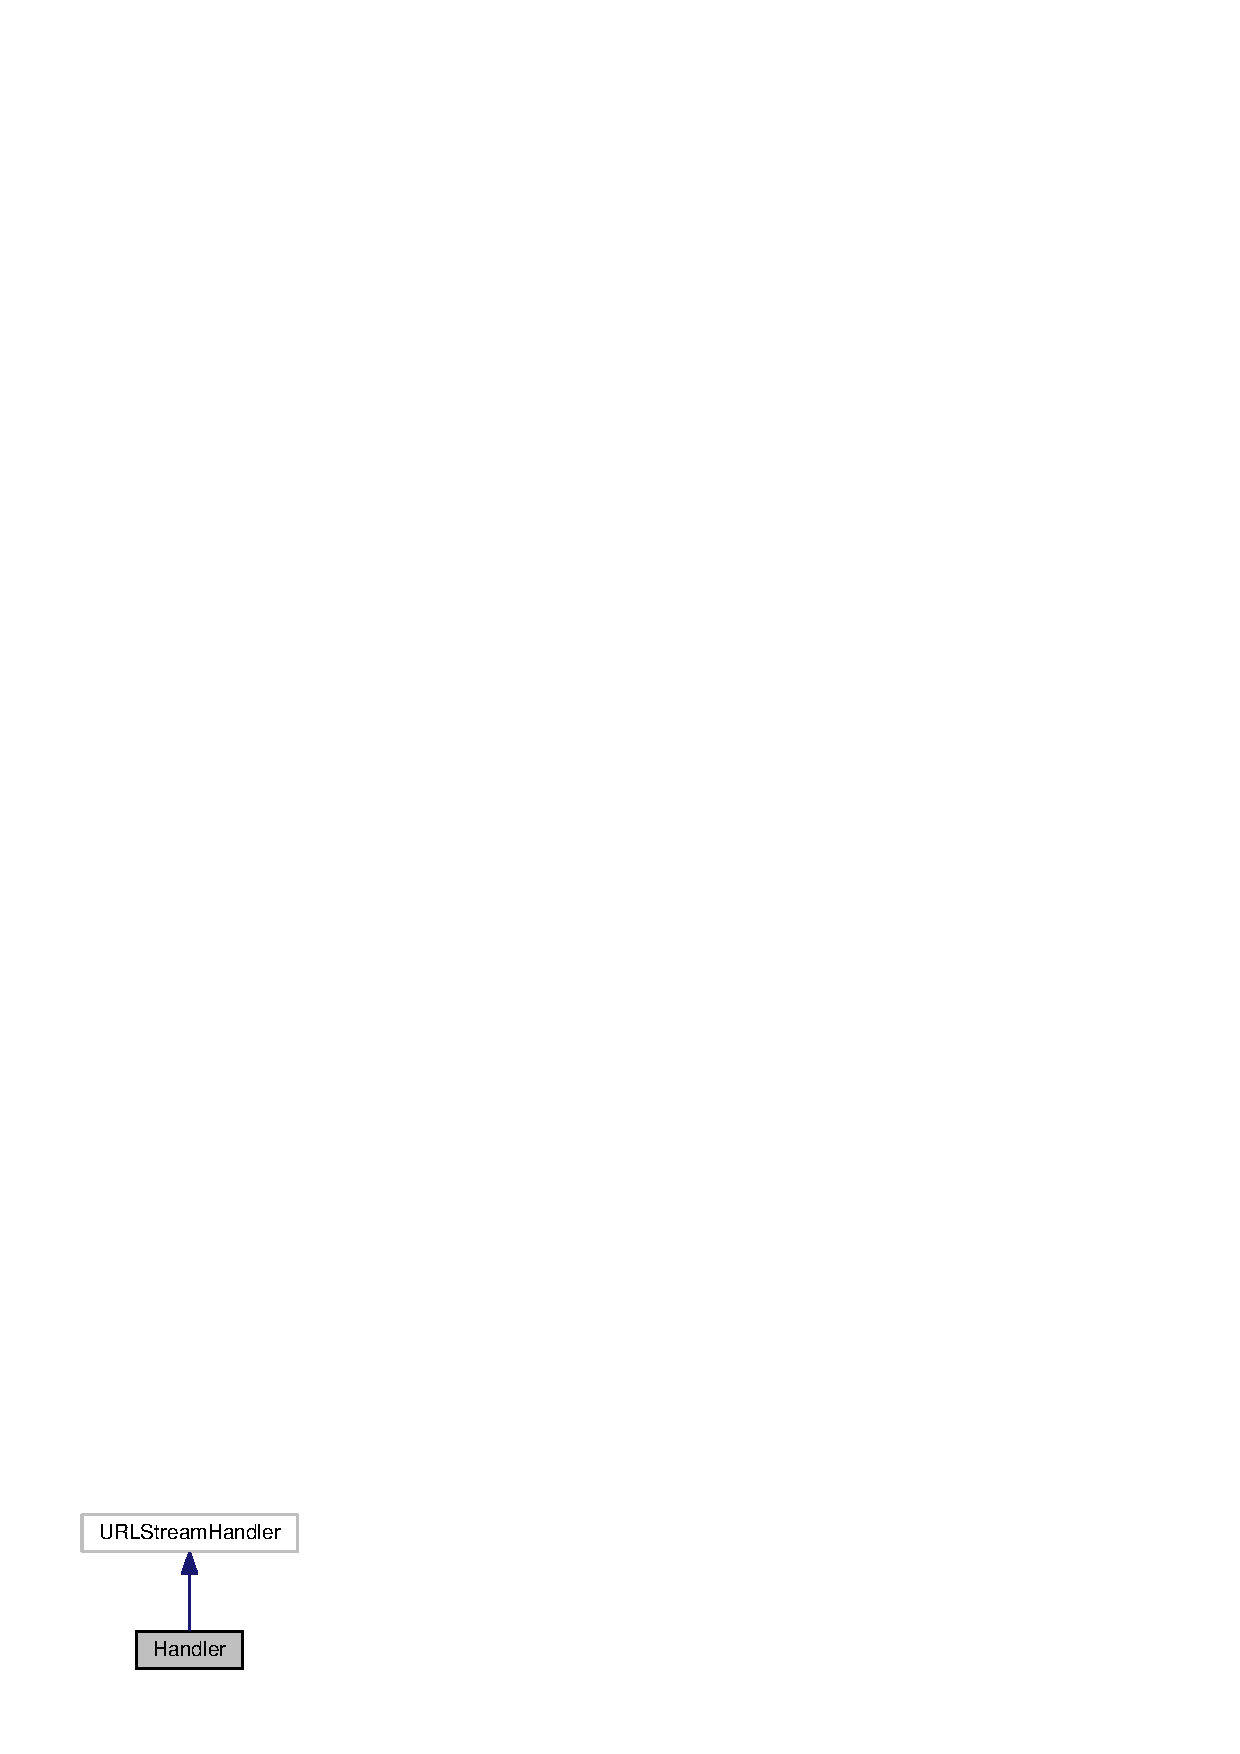
\includegraphics[width=146pt]{classorg_1_1smallfoot_1_1parser_1_1dcfm_1_1Handler__coll__graph}
\end{center}
\end{figure}
\subsection*{Protected Member Functions}
\begin{DoxyCompactItemize}
\item 
U\+R\+L\+Connection {\bf open\+Connection} (U\+R\+L url)
\begin{DoxyCompactList}\small\item\em \doxyref{open\+Connection(\+U\+R\+L)}{p.}{classorg_1_1smallfoot_1_1parser_1_1dcfm_1_1Handler_a3838795af42df5d7757e609b8b312956} overrides java.\+net.\+U\+R\+L\+Stream\+Handler.\+open\+Connection(\+U\+R\+L) by wrapping a proper connection with prototype-\/matching call and parameters \end{DoxyCompactList}\item 
int {\bf get\+Default\+Port} ()
\end{DoxyCompactItemize}


\subsection{Detailed Description}


Definition at line 21 of file Handler.\+java.



\subsection{Member Function Documentation}
\index{org\+::smallfoot\+::parser\+::dcfm\+::\+Handler@{org\+::smallfoot\+::parser\+::dcfm\+::\+Handler}!get\+Default\+Port@{get\+Default\+Port}}
\index{get\+Default\+Port@{get\+Default\+Port}!org\+::smallfoot\+::parser\+::dcfm\+::\+Handler@{org\+::smallfoot\+::parser\+::dcfm\+::\+Handler}}
\subsubsection[{get\+Default\+Port}]{\setlength{\rightskip}{0pt plus 5cm}int get\+Default\+Port (
\begin{DoxyParamCaption}
{}
\end{DoxyParamCaption}
)\hspace{0.3cm}{\ttfamily [inline]}, {\ttfamily [protected]}}\label{classorg_1_1smallfoot_1_1parser_1_1dcfm_1_1Handler_aadc354b6a8746020e9961fbcb433427c}


Definition at line 34 of file Handler.\+java.

\index{org\+::smallfoot\+::parser\+::dcfm\+::\+Handler@{org\+::smallfoot\+::parser\+::dcfm\+::\+Handler}!open\+Connection@{open\+Connection}}
\index{open\+Connection@{open\+Connection}!org\+::smallfoot\+::parser\+::dcfm\+::\+Handler@{org\+::smallfoot\+::parser\+::dcfm\+::\+Handler}}
\subsubsection[{open\+Connection}]{\setlength{\rightskip}{0pt plus 5cm}U\+R\+L\+Connection open\+Connection (
\begin{DoxyParamCaption}
\item[{U\+R\+L}]{url}
\end{DoxyParamCaption}
)\hspace{0.3cm}{\ttfamily [inline]}, {\ttfamily [protected]}}\label{classorg_1_1smallfoot_1_1parser_1_1dcfm_1_1Handler_a3838795af42df5d7757e609b8b312956}


\doxyref{open\+Connection(\+U\+R\+L)}{p.}{classorg_1_1smallfoot_1_1parser_1_1dcfm_1_1Handler_a3838795af42df5d7757e609b8b312956} overrides java.\+net.\+U\+R\+L\+Stream\+Handler.\+open\+Connection(\+U\+R\+L) by wrapping a proper connection with prototype-\/matching call and parameters 

\begin{DoxyReturn}{Returns}
populated connection as \doxyref{org.\+smallfoot.\+parser.\+bnapsql.\+B\+N\+A\+P\+U\+R\+L\+Connection(\+Connection)}{p.}{classorg_1_1smallfoot_1_1parser_1_1bnapsql_1_1BNAPURLConnection} 
\end{DoxyReturn}

\begin{DoxyParams}{Parameters}
{\em url} & U\+R\+L to which we need to connect \\
\hline
\end{DoxyParams}


Definition at line 29 of file Handler.\+java.



The documentation for this class was generated from the following file\+:\begin{DoxyCompactItemize}
\item 
java/genproto/dcfm/{\bf Handler.\+java}\end{DoxyCompactItemize}

\section{Handler Class Reference}
\label{classorg_1_1smallfoot_1_1parser_1_1msosmsql_1_1Handler}\index{Handler@{Handler}}


Inheritance diagram for Handler\+:\nopagebreak
\begin{figure}[H]
\begin{center}
\leavevmode
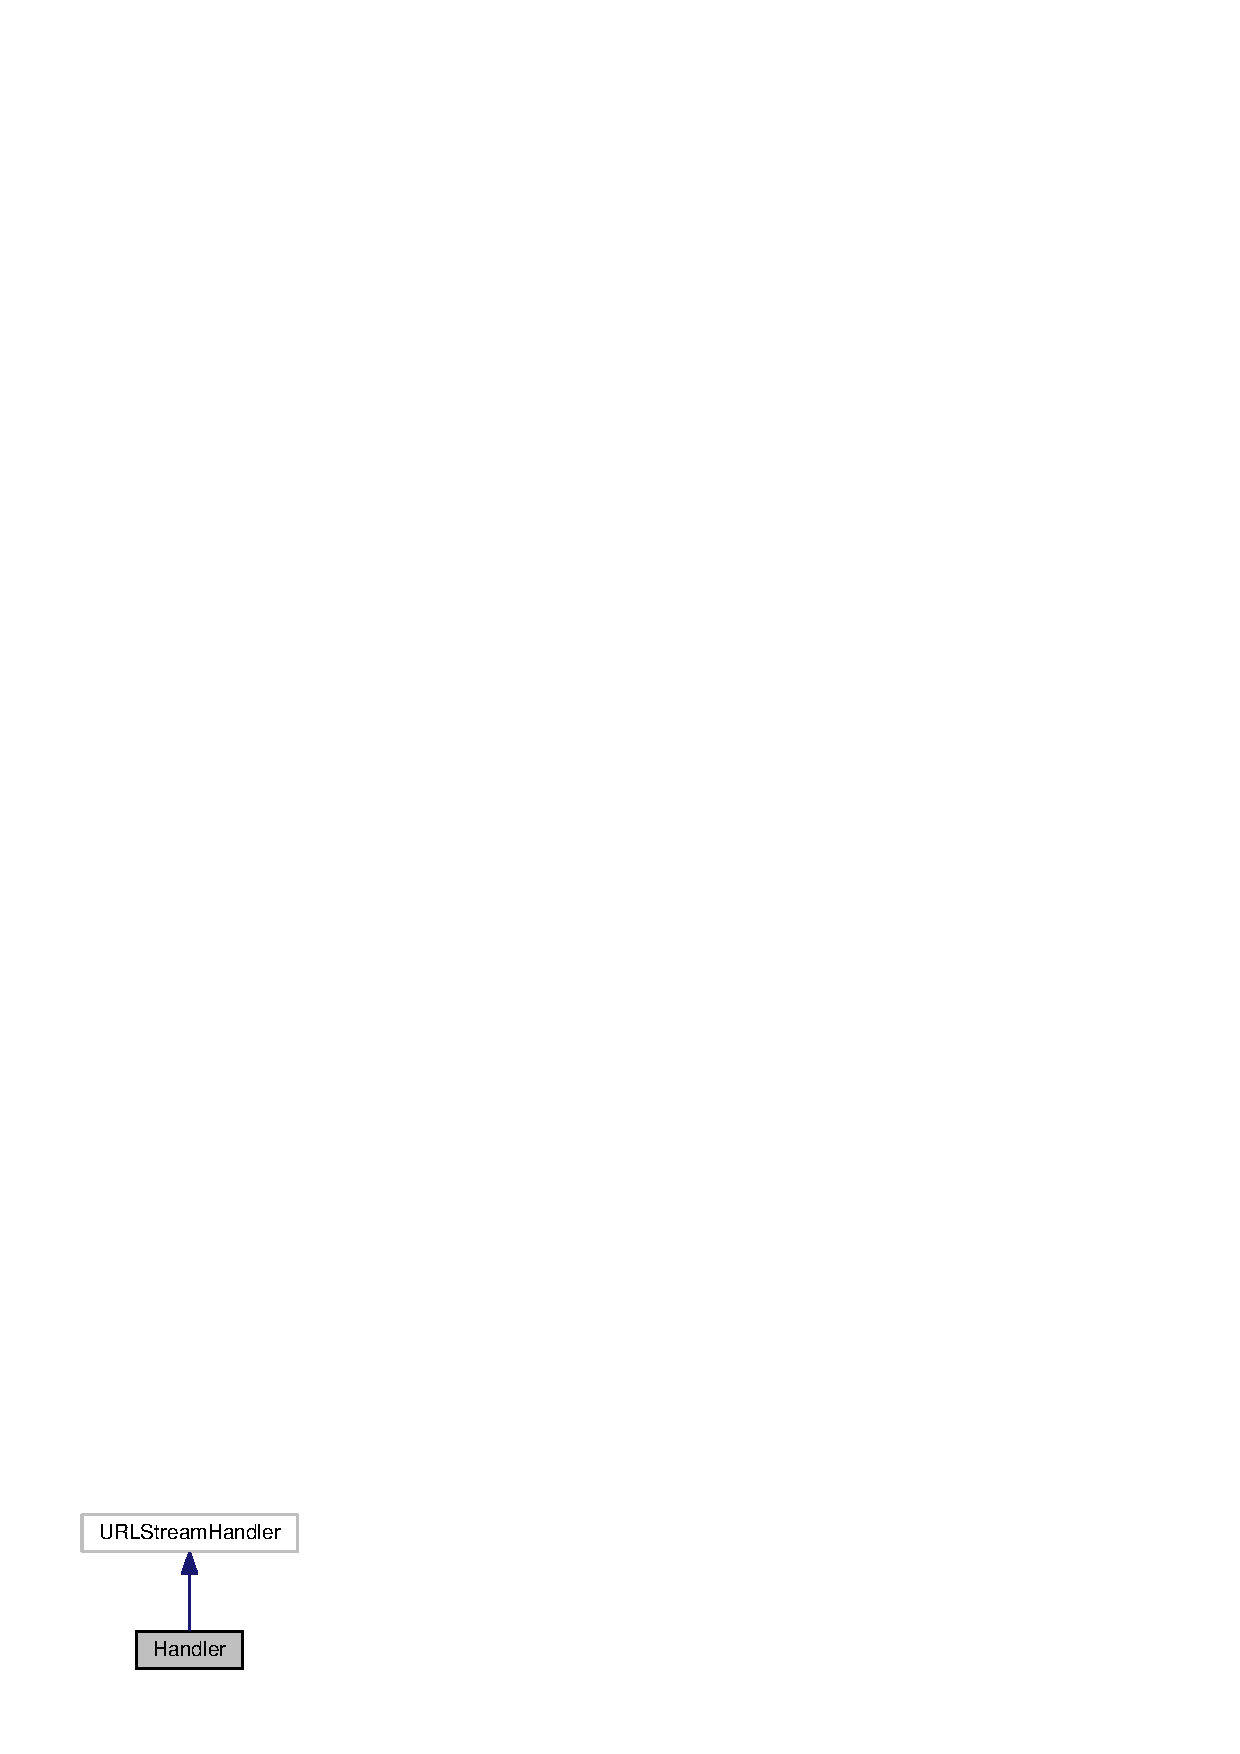
\includegraphics[width=146pt]{classorg_1_1smallfoot_1_1parser_1_1msosmsql_1_1Handler__inherit__graph}
\end{center}
\end{figure}


Collaboration diagram for Handler\+:\nopagebreak
\begin{figure}[H]
\begin{center}
\leavevmode
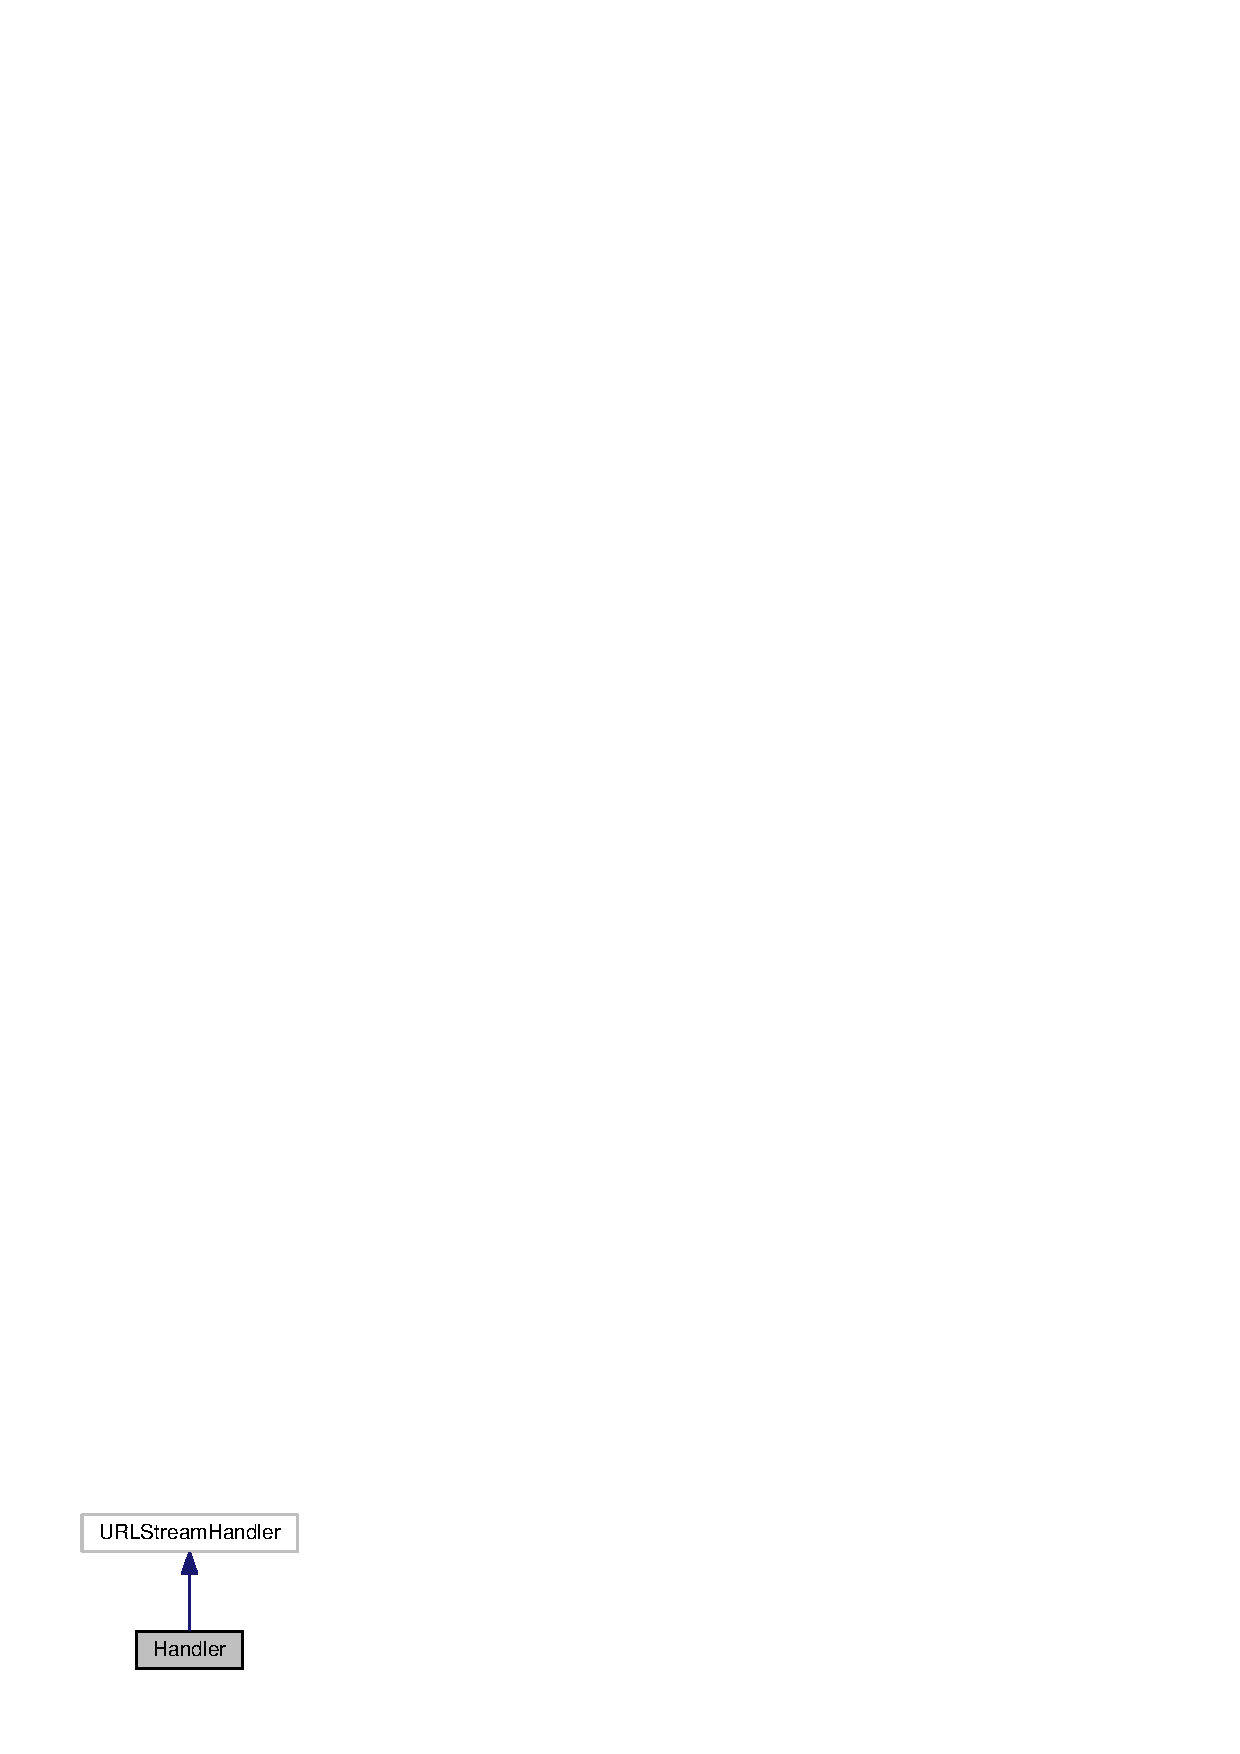
\includegraphics[width=146pt]{classorg_1_1smallfoot_1_1parser_1_1msosmsql_1_1Handler__coll__graph}
\end{center}
\end{figure}
\subsection*{Protected Member Functions}
\begin{DoxyCompactItemize}
\item 
U\+R\+L\+Connection {\bf open\+Connection} (U\+R\+L url)
\begin{DoxyCompactList}\small\item\em \doxyref{open\+Connection(\+U\+R\+L)}{p.}{classorg_1_1smallfoot_1_1parser_1_1msosmsql_1_1Handler_a3838795af42df5d7757e609b8b312956} overrides java.\+net.\+U\+R\+L\+Stream\+Handler.\+open\+Connection(\+U\+R\+L) by wrapping a proper connection with prototype-\/matching call and parameters \end{DoxyCompactList}\item 
int {\bf get\+Default\+Port} ()
\end{DoxyCompactItemize}


\subsection{Detailed Description}


Definition at line 21 of file Handler.\+java.



\subsection{Member Function Documentation}
\index{org\+::smallfoot\+::parser\+::msosmsql\+::\+Handler@{org\+::smallfoot\+::parser\+::msosmsql\+::\+Handler}!get\+Default\+Port@{get\+Default\+Port}}
\index{get\+Default\+Port@{get\+Default\+Port}!org\+::smallfoot\+::parser\+::msosmsql\+::\+Handler@{org\+::smallfoot\+::parser\+::msosmsql\+::\+Handler}}
\subsubsection[{get\+Default\+Port}]{\setlength{\rightskip}{0pt plus 5cm}int get\+Default\+Port (
\begin{DoxyParamCaption}
{}
\end{DoxyParamCaption}
)\hspace{0.3cm}{\ttfamily [inline]}, {\ttfamily [protected]}}\label{classorg_1_1smallfoot_1_1parser_1_1msosmsql_1_1Handler_aadc354b6a8746020e9961fbcb433427c}


Definition at line 34 of file Handler.\+java.

\index{org\+::smallfoot\+::parser\+::msosmsql\+::\+Handler@{org\+::smallfoot\+::parser\+::msosmsql\+::\+Handler}!open\+Connection@{open\+Connection}}
\index{open\+Connection@{open\+Connection}!org\+::smallfoot\+::parser\+::msosmsql\+::\+Handler@{org\+::smallfoot\+::parser\+::msosmsql\+::\+Handler}}
\subsubsection[{open\+Connection}]{\setlength{\rightskip}{0pt plus 5cm}U\+R\+L\+Connection open\+Connection (
\begin{DoxyParamCaption}
\item[{U\+R\+L}]{url}
\end{DoxyParamCaption}
)\hspace{0.3cm}{\ttfamily [inline]}, {\ttfamily [protected]}}\label{classorg_1_1smallfoot_1_1parser_1_1msosmsql_1_1Handler_a3838795af42df5d7757e609b8b312956}


\doxyref{open\+Connection(\+U\+R\+L)}{p.}{classorg_1_1smallfoot_1_1parser_1_1msosmsql_1_1Handler_a3838795af42df5d7757e609b8b312956} overrides java.\+net.\+U\+R\+L\+Stream\+Handler.\+open\+Connection(\+U\+R\+L) by wrapping a proper connection with prototype-\/matching call and parameters 

\begin{DoxyReturn}{Returns}
populated connection as \doxyref{org.\+smallfoot.\+parser.\+msosmsql.\+M\+S\+D\+W\+H\+U\+R\+L\+Connection(\+Connection)}{p.}{classorg_1_1smallfoot_1_1parser_1_1msosmsql_1_1MSDWHURLConnection} 
\end{DoxyReturn}

\begin{DoxyParams}{Parameters}
{\em url} & U\+R\+L to which we need to connect \\
\hline
\end{DoxyParams}


Definition at line 29 of file Handler.\+java.



The documentation for this class was generated from the following file\+:\begin{DoxyCompactItemize}
\item 
java/genproto/msosmsql/{\bf Handler.\+java}\end{DoxyCompactItemize}

\section{Handler Class Reference}
\label{classorg_1_1smallfoot_1_1parser_1_1bnapsql_1_1Handler}\index{Handler@{Handler}}


Inheritance diagram for Handler\+:\nopagebreak
\begin{figure}[H]
\begin{center}
\leavevmode
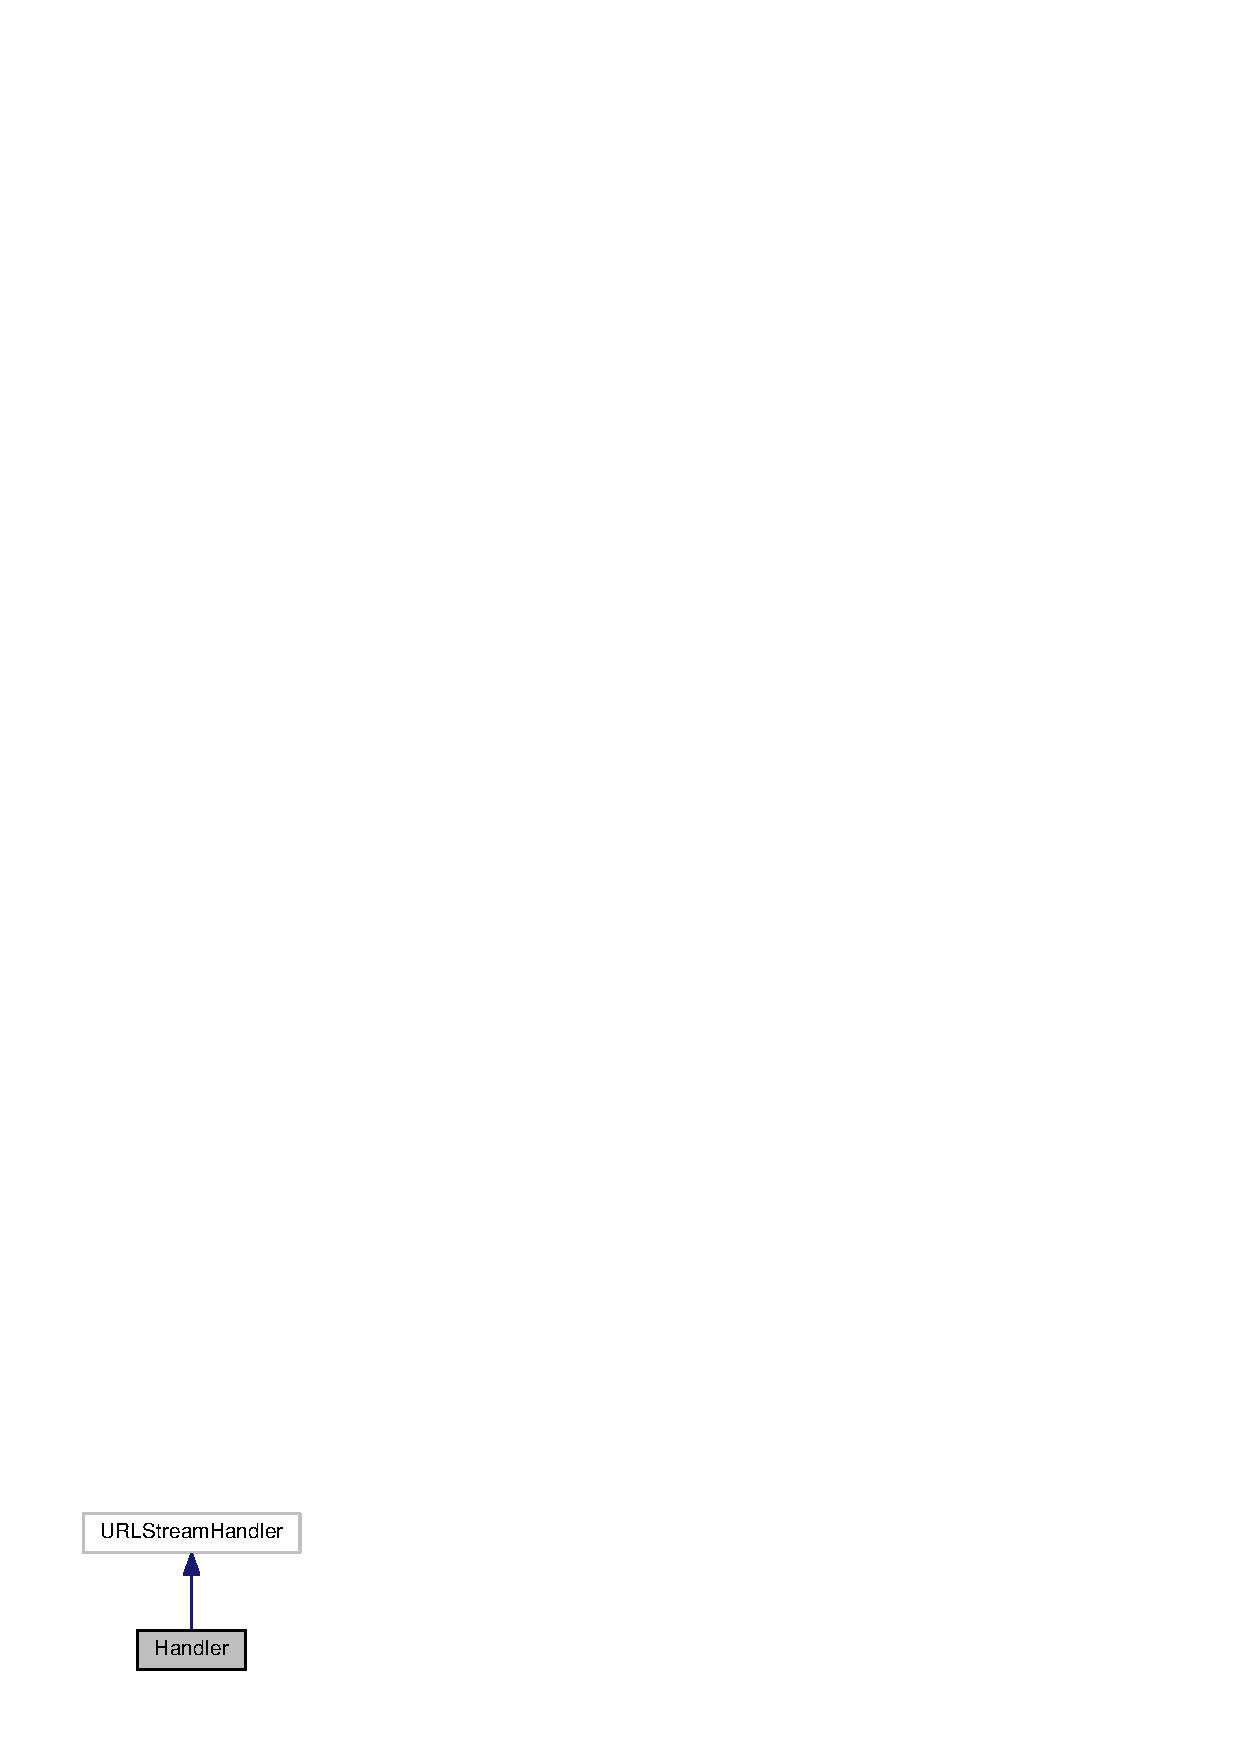
\includegraphics[width=146pt]{classorg_1_1smallfoot_1_1parser_1_1bnapsql_1_1Handler__inherit__graph}
\end{center}
\end{figure}


Collaboration diagram for Handler\+:\nopagebreak
\begin{figure}[H]
\begin{center}
\leavevmode
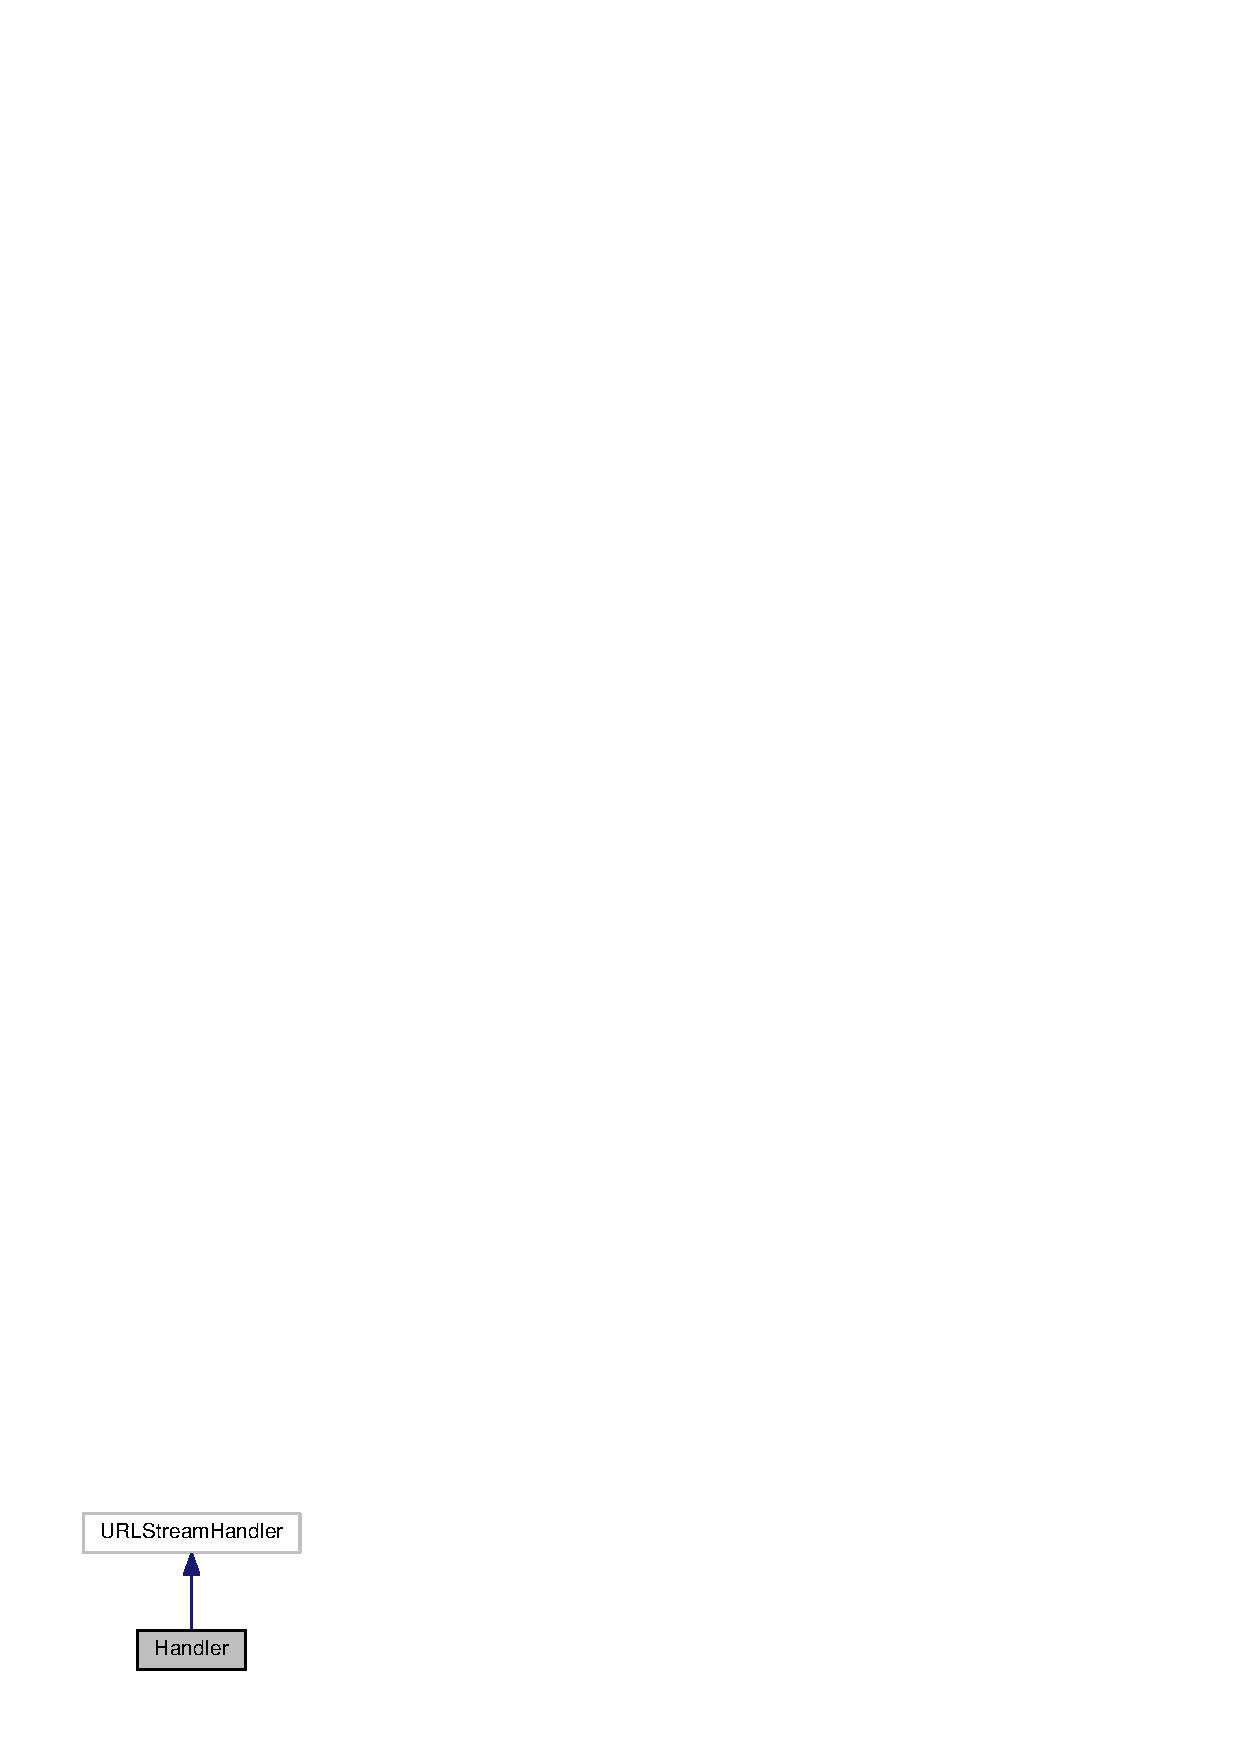
\includegraphics[width=146pt]{classorg_1_1smallfoot_1_1parser_1_1bnapsql_1_1Handler__coll__graph}
\end{center}
\end{figure}
\subsection*{Protected Member Functions}
\begin{DoxyCompactItemize}
\item 
U\+R\+L\+Connection {\bf open\+Connection} (U\+R\+L url)
\begin{DoxyCompactList}\small\item\em \doxyref{open\+Connection(\+U\+R\+L)}{p.}{classorg_1_1smallfoot_1_1parser_1_1bnapsql_1_1Handler_a3838795af42df5d7757e609b8b312956} overrides java.\+net.\+U\+R\+L\+Stream\+Handler.\+open\+Connection(\+U\+R\+L) by wrapping a proper connection with prototype-\/matching call and parameters \end{DoxyCompactList}\end{DoxyCompactItemize}


\subsection{Detailed Description}


Definition at line 21 of file Handler.\+java.



\subsection{Member Function Documentation}
\index{org\+::smallfoot\+::parser\+::bnapsql\+::\+Handler@{org\+::smallfoot\+::parser\+::bnapsql\+::\+Handler}!open\+Connection@{open\+Connection}}
\index{open\+Connection@{open\+Connection}!org\+::smallfoot\+::parser\+::bnapsql\+::\+Handler@{org\+::smallfoot\+::parser\+::bnapsql\+::\+Handler}}
\subsubsection[{open\+Connection}]{\setlength{\rightskip}{0pt plus 5cm}U\+R\+L\+Connection open\+Connection (
\begin{DoxyParamCaption}
\item[{U\+R\+L}]{url}
\end{DoxyParamCaption}
)\hspace{0.3cm}{\ttfamily [inline]}, {\ttfamily [protected]}}\label{classorg_1_1smallfoot_1_1parser_1_1bnapsql_1_1Handler_a3838795af42df5d7757e609b8b312956}


\doxyref{open\+Connection(\+U\+R\+L)}{p.}{classorg_1_1smallfoot_1_1parser_1_1bnapsql_1_1Handler_a3838795af42df5d7757e609b8b312956} overrides java.\+net.\+U\+R\+L\+Stream\+Handler.\+open\+Connection(\+U\+R\+L) by wrapping a proper connection with prototype-\/matching call and parameters 

\begin{DoxyReturn}{Returns}
populated connection as \doxyref{org.\+smallfoot.\+parser.\+bnapsql.\+B\+N\+A\+P\+U\+R\+L\+Connection(\+Connection)}{p.}{classorg_1_1smallfoot_1_1parser_1_1bnapsql_1_1BNAPURLConnection} 
\end{DoxyReturn}

\begin{DoxyParams}{Parameters}
{\em url} & U\+R\+L to which we need to connect \\
\hline
\end{DoxyParams}


Definition at line 29 of file Handler.\+java.



The documentation for this class was generated from the following file\+:\begin{DoxyCompactItemize}
\item 
java/genproto/bnapsql/{\bf Handler.\+java}\end{DoxyCompactItemize}

\section{Handler Class Reference}
\label{classorg_1_1smallfoot_1_1parser_1_1ocidwh_1_1Handler}\index{Handler@{Handler}}


Inheritance diagram for Handler\+:\nopagebreak
\begin{figure}[H]
\begin{center}
\leavevmode
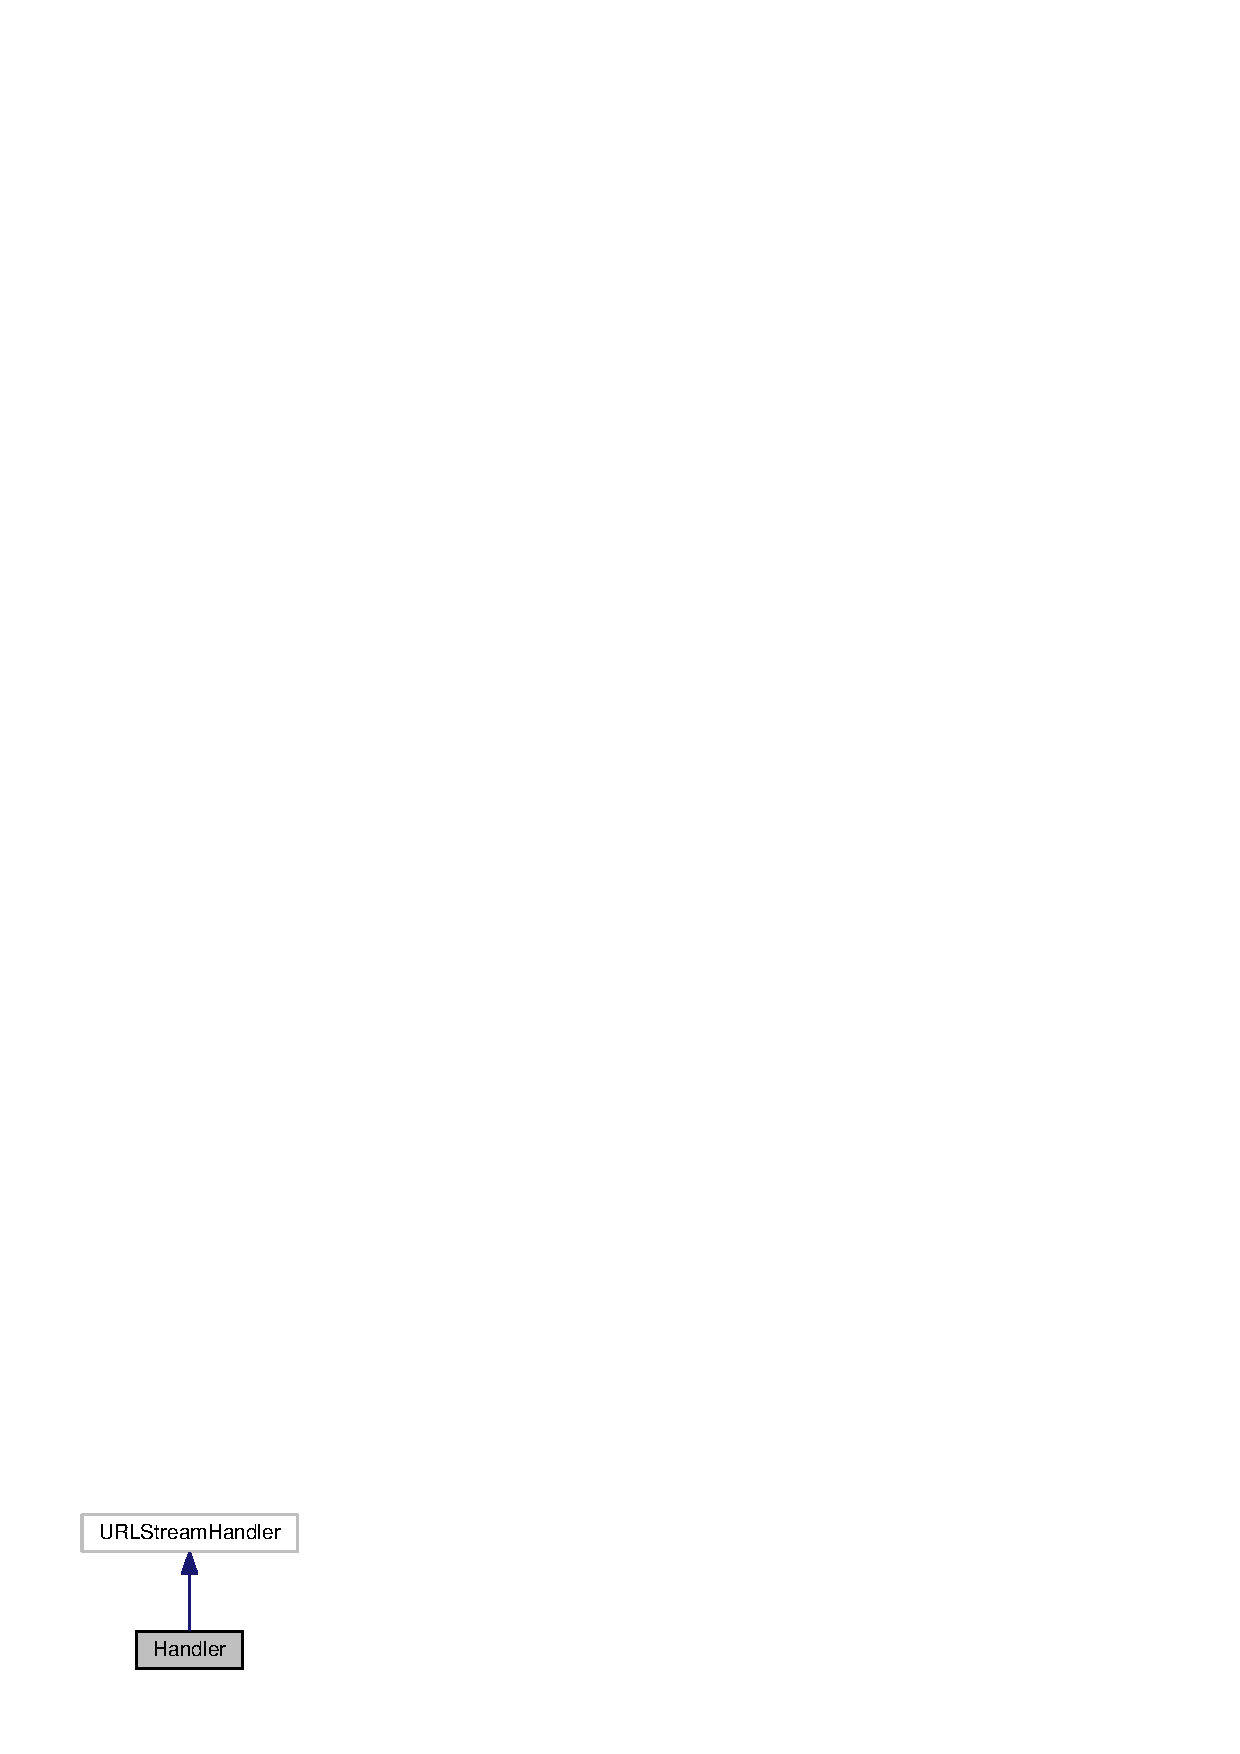
\includegraphics[width=146pt]{classorg_1_1smallfoot_1_1parser_1_1ocidwh_1_1Handler__inherit__graph}
\end{center}
\end{figure}


Collaboration diagram for Handler\+:\nopagebreak
\begin{figure}[H]
\begin{center}
\leavevmode
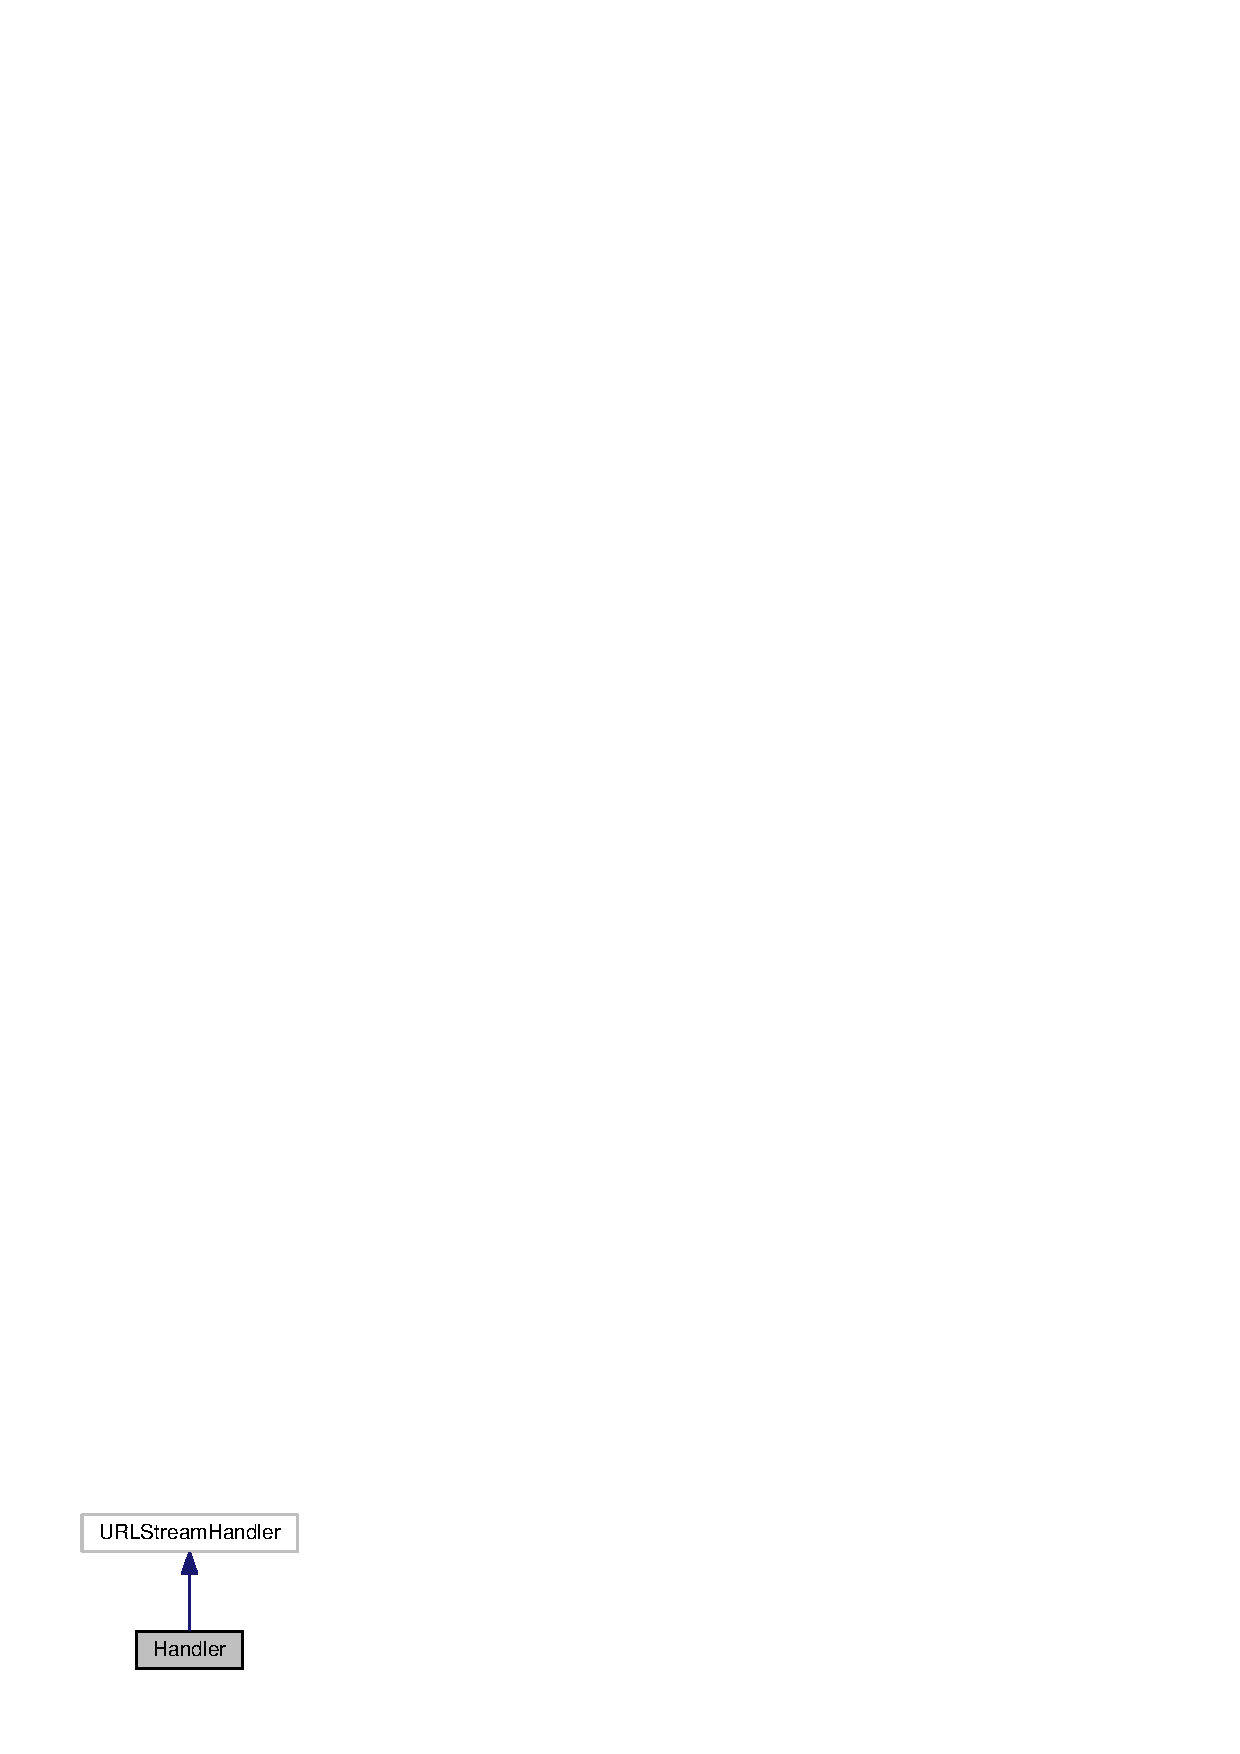
\includegraphics[width=146pt]{classorg_1_1smallfoot_1_1parser_1_1ocidwh_1_1Handler__coll__graph}
\end{center}
\end{figure}
\subsection*{Protected Member Functions}
\begin{DoxyCompactItemize}
\item 
U\+R\+L\+Connection {\bf open\+Connection} (U\+R\+L url)
\begin{DoxyCompactList}\small\item\em \doxyref{open\+Connection(\+U\+R\+L)}{p.}{classorg_1_1smallfoot_1_1parser_1_1ocidwh_1_1Handler_a3838795af42df5d7757e609b8b312956} overrides java.\+net.\+U\+R\+L\+Stream\+Handler.\+open\+Connection(\+U\+R\+L) by wrapping a proper connection with prototype-\/matching call and parameters \end{DoxyCompactList}\item 
int {\bf get\+Default\+Port} ()
\end{DoxyCompactItemize}


\subsection{Detailed Description}


Definition at line 21 of file Handler.\+java.



\subsection{Member Function Documentation}
\index{org\+::smallfoot\+::parser\+::ocidwh\+::\+Handler@{org\+::smallfoot\+::parser\+::ocidwh\+::\+Handler}!get\+Default\+Port@{get\+Default\+Port}}
\index{get\+Default\+Port@{get\+Default\+Port}!org\+::smallfoot\+::parser\+::ocidwh\+::\+Handler@{org\+::smallfoot\+::parser\+::ocidwh\+::\+Handler}}
\subsubsection[{get\+Default\+Port}]{\setlength{\rightskip}{0pt plus 5cm}int get\+Default\+Port (
\begin{DoxyParamCaption}
{}
\end{DoxyParamCaption}
)\hspace{0.3cm}{\ttfamily [inline]}, {\ttfamily [protected]}}\label{classorg_1_1smallfoot_1_1parser_1_1ocidwh_1_1Handler_aadc354b6a8746020e9961fbcb433427c}


Definition at line 34 of file Handler.\+java.

\index{org\+::smallfoot\+::parser\+::ocidwh\+::\+Handler@{org\+::smallfoot\+::parser\+::ocidwh\+::\+Handler}!open\+Connection@{open\+Connection}}
\index{open\+Connection@{open\+Connection}!org\+::smallfoot\+::parser\+::ocidwh\+::\+Handler@{org\+::smallfoot\+::parser\+::ocidwh\+::\+Handler}}
\subsubsection[{open\+Connection}]{\setlength{\rightskip}{0pt plus 5cm}U\+R\+L\+Connection open\+Connection (
\begin{DoxyParamCaption}
\item[{U\+R\+L}]{url}
\end{DoxyParamCaption}
)\hspace{0.3cm}{\ttfamily [inline]}, {\ttfamily [protected]}}\label{classorg_1_1smallfoot_1_1parser_1_1ocidwh_1_1Handler_a3838795af42df5d7757e609b8b312956}


\doxyref{open\+Connection(\+U\+R\+L)}{p.}{classorg_1_1smallfoot_1_1parser_1_1ocidwh_1_1Handler_a3838795af42df5d7757e609b8b312956} overrides java.\+net.\+U\+R\+L\+Stream\+Handler.\+open\+Connection(\+U\+R\+L) by wrapping a proper connection with prototype-\/matching call and parameters 

\begin{DoxyReturn}{Returns}
populated connection as \doxyref{org.\+smallfoot.\+parser.\+ocidwh.\+D\+W\+H\+U\+R\+L\+Connection(\+Connection)}{p.}{classorg_1_1smallfoot_1_1parser_1_1ocidwh_1_1DWHURLConnection} 
\end{DoxyReturn}

\begin{DoxyParams}{Parameters}
{\em url} & U\+R\+L to which we need to connect \\
\hline
\end{DoxyParams}


Definition at line 29 of file Handler.\+java.



The documentation for this class was generated from the following file\+:\begin{DoxyCompactItemize}
\item 
java/genproto/ocidwh/{\bf Handler.\+java}\end{DoxyCompactItemize}

\section{M\+S\+D\+W\+H\+U\+R\+L\+Connection Class Reference}
\label{classorg_1_1smallfoot_1_1parser_1_1msosmsql_1_1MSDWHURLConnection}\index{M\+S\+D\+W\+H\+U\+R\+L\+Connection@{M\+S\+D\+W\+H\+U\+R\+L\+Connection}}


Inheritance diagram for M\+S\+D\+W\+H\+U\+R\+L\+Connection\+:\nopagebreak
\begin{figure}[H]
\begin{center}
\leavevmode
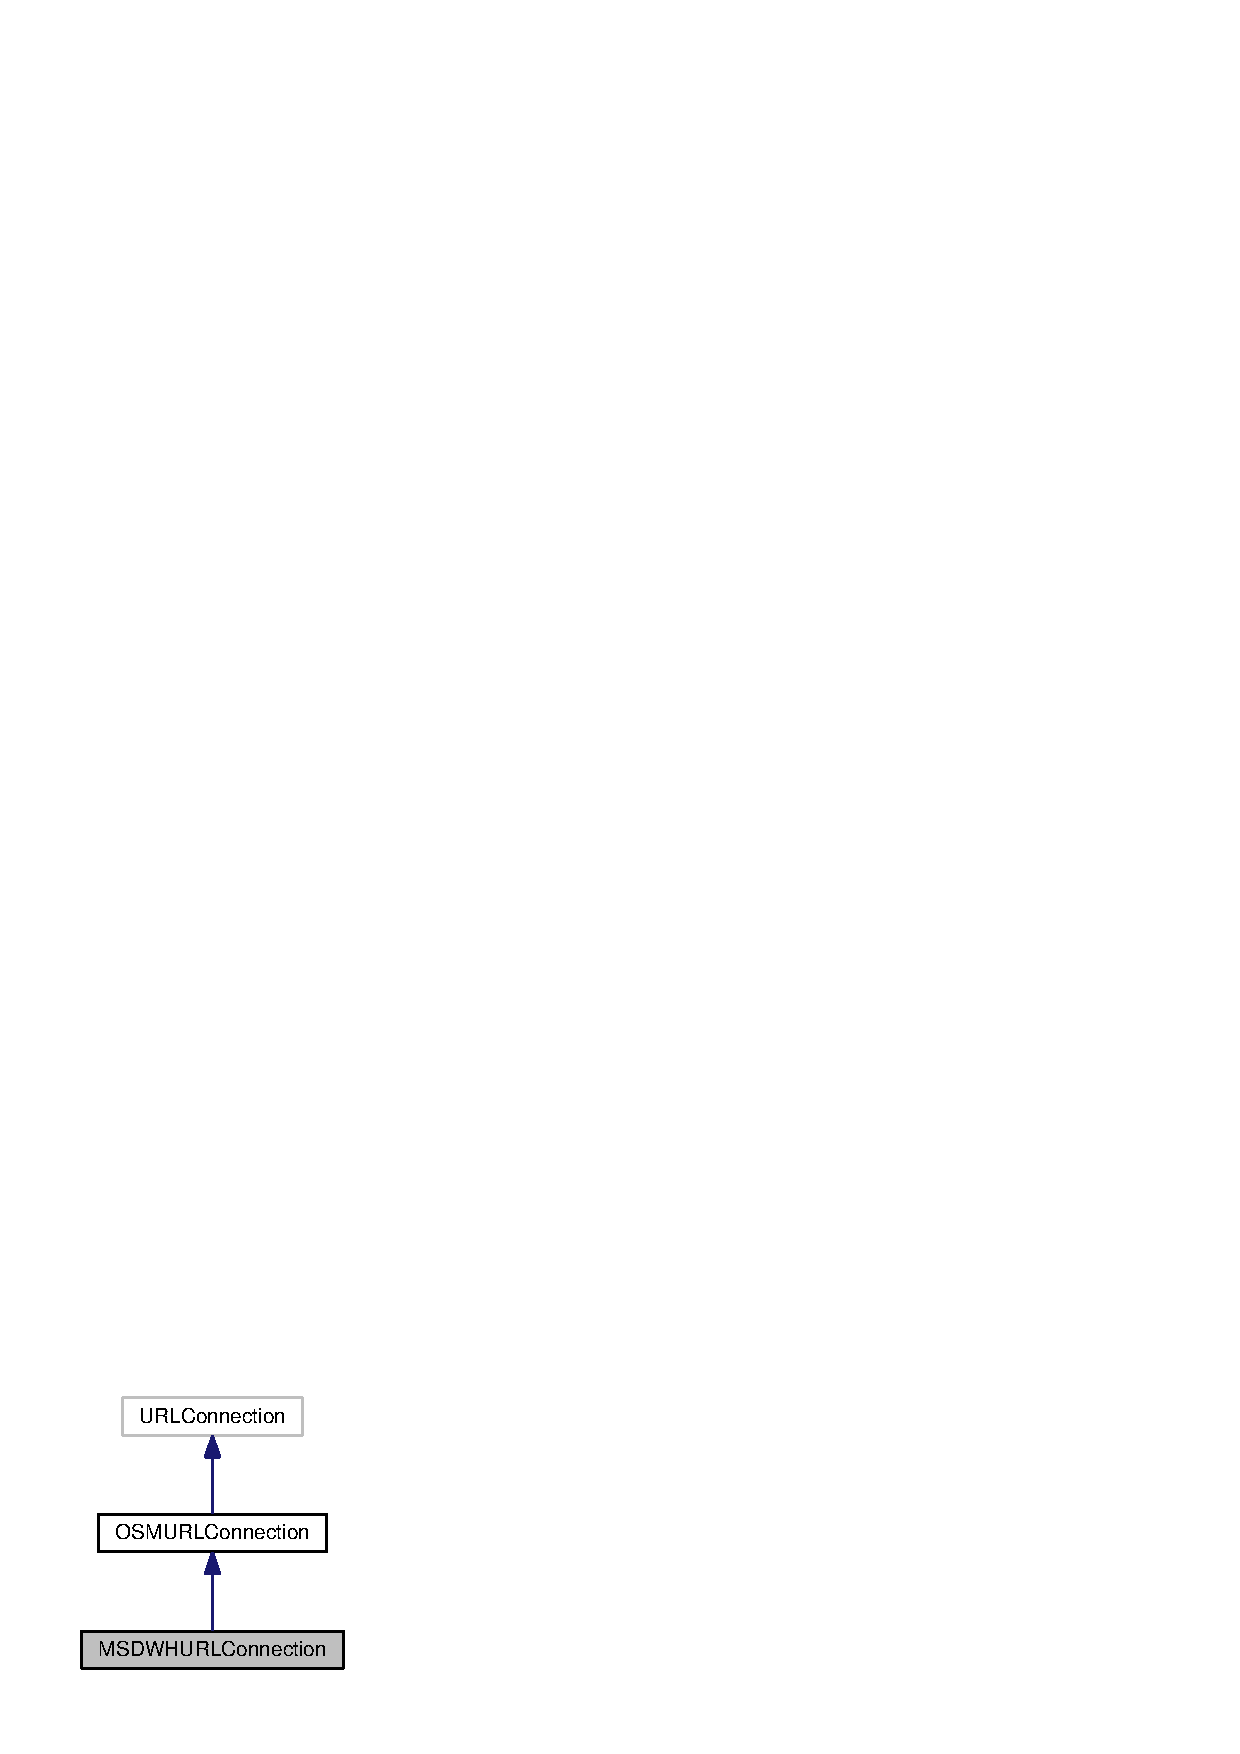
\includegraphics[width=168pt]{classorg_1_1smallfoot_1_1parser_1_1msosmsql_1_1MSDWHURLConnection__inherit__graph}
\end{center}
\end{figure}


Collaboration diagram for M\+S\+D\+W\+H\+U\+R\+L\+Connection\+:\nopagebreak
\begin{figure}[H]
\begin{center}
\leavevmode
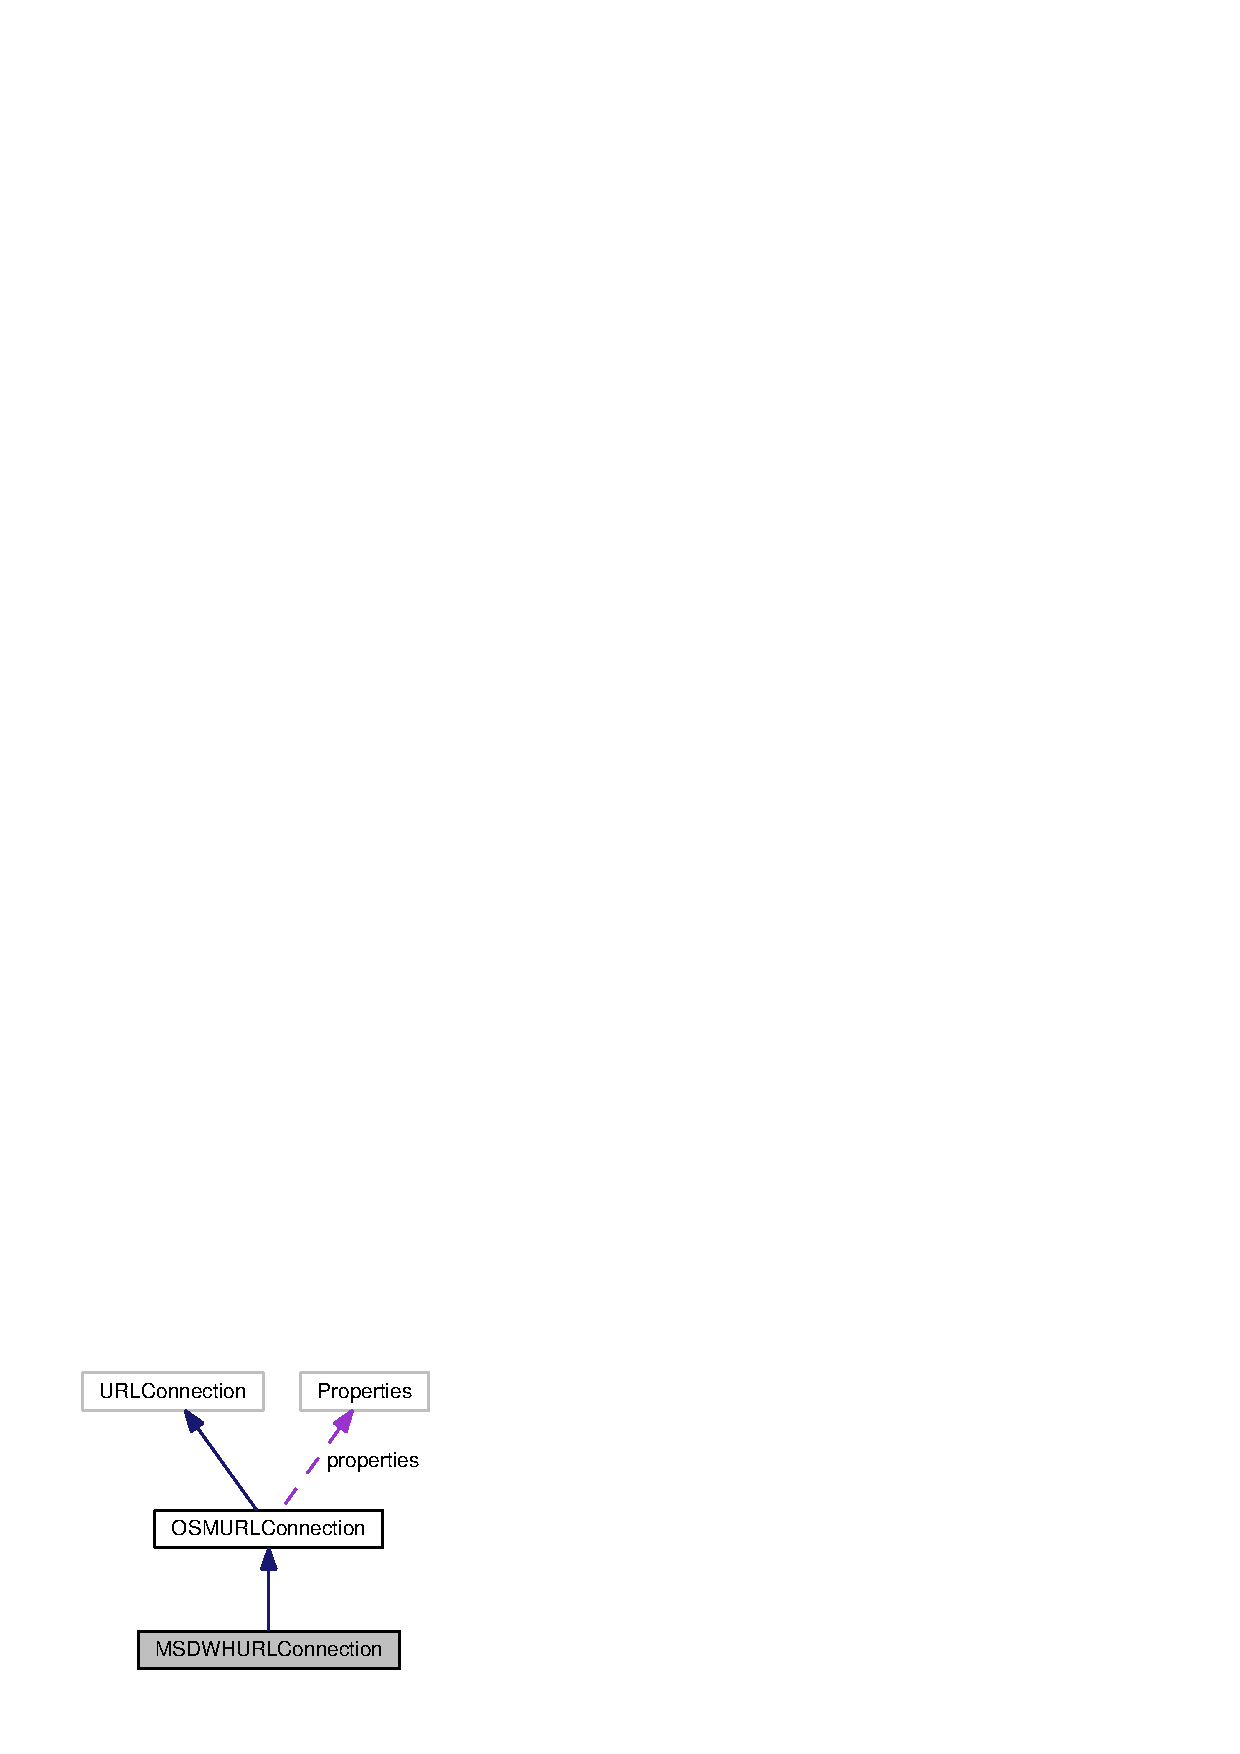
\includegraphics[width=209pt]{classorg_1_1smallfoot_1_1parser_1_1msosmsql_1_1MSDWHURLConnection__coll__graph}
\end{center}
\end{figure}
\subsection*{Data Structures}
\begin{DoxyCompactItemize}
\item 
class {\bf M\+S\+Result\+C\+S\+V\+Pipe}
\begin{DoxyCompactList}\small\item\em Piped\+Output\+Stream to push out resultsets as C\+S\+V Nicknames. \end{DoxyCompactList}\end{DoxyCompactItemize}
\subsection*{Public Member Functions}
\begin{DoxyCompactItemize}
\item 
{\bf M\+S\+D\+W\+H\+U\+R\+L\+Connection} (String connection\+Info, String username, String password)
\item 
{\bf M\+S\+D\+W\+H\+U\+R\+L\+Connection} (java.\+net.\+U\+R\+L url)
\item 
java.\+io.\+Input\+Stream {\bf get\+Input\+Stream} ()
\begin{DoxyCompactList}\small\item\em connect the result of a \end{DoxyCompactList}\end{DoxyCompactItemize}
\subsection*{Additional Inherited Members}


\subsection{Detailed Description}


Definition at line 25 of file M\+S\+D\+W\+H\+U\+R\+L\+Connection.\+java.



\subsection{Constructor \& Destructor Documentation}
\index{org\+::smallfoot\+::parser\+::msosmsql\+::\+M\+S\+D\+W\+H\+U\+R\+L\+Connection@{org\+::smallfoot\+::parser\+::msosmsql\+::\+M\+S\+D\+W\+H\+U\+R\+L\+Connection}!M\+S\+D\+W\+H\+U\+R\+L\+Connection@{M\+S\+D\+W\+H\+U\+R\+L\+Connection}}
\index{M\+S\+D\+W\+H\+U\+R\+L\+Connection@{M\+S\+D\+W\+H\+U\+R\+L\+Connection}!org\+::smallfoot\+::parser\+::msosmsql\+::\+M\+S\+D\+W\+H\+U\+R\+L\+Connection@{org\+::smallfoot\+::parser\+::msosmsql\+::\+M\+S\+D\+W\+H\+U\+R\+L\+Connection}}
\subsubsection[{M\+S\+D\+W\+H\+U\+R\+L\+Connection}]{\setlength{\rightskip}{0pt plus 5cm}{\bf M\+S\+D\+W\+H\+U\+R\+L\+Connection} (
\begin{DoxyParamCaption}
\item[{String}]{connection\+Info, }
\item[{String}]{username, }
\item[{String}]{password}
\end{DoxyParamCaption}
)\hspace{0.3cm}{\ttfamily [inline]}}\label{classorg_1_1smallfoot_1_1parser_1_1msosmsql_1_1MSDWHURLConnection_a658c89e45145229c94d261bdbaa085b2}


Definition at line 27 of file M\+S\+D\+W\+H\+U\+R\+L\+Connection.\+java.

\index{org\+::smallfoot\+::parser\+::msosmsql\+::\+M\+S\+D\+W\+H\+U\+R\+L\+Connection@{org\+::smallfoot\+::parser\+::msosmsql\+::\+M\+S\+D\+W\+H\+U\+R\+L\+Connection}!M\+S\+D\+W\+H\+U\+R\+L\+Connection@{M\+S\+D\+W\+H\+U\+R\+L\+Connection}}
\index{M\+S\+D\+W\+H\+U\+R\+L\+Connection@{M\+S\+D\+W\+H\+U\+R\+L\+Connection}!org\+::smallfoot\+::parser\+::msosmsql\+::\+M\+S\+D\+W\+H\+U\+R\+L\+Connection@{org\+::smallfoot\+::parser\+::msosmsql\+::\+M\+S\+D\+W\+H\+U\+R\+L\+Connection}}
\subsubsection[{M\+S\+D\+W\+H\+U\+R\+L\+Connection}]{\setlength{\rightskip}{0pt plus 5cm}{\bf M\+S\+D\+W\+H\+U\+R\+L\+Connection} (
\begin{DoxyParamCaption}
\item[{java.\+net.\+U\+R\+L}]{url}
\end{DoxyParamCaption}
)\hspace{0.3cm}{\ttfamily [inline]}}\label{classorg_1_1smallfoot_1_1parser_1_1msosmsql_1_1MSDWHURLConnection_abae9d7254fdf3bbe668232e54188a03f}


Definition at line 32 of file M\+S\+D\+W\+H\+U\+R\+L\+Connection.\+java.



\subsection{Member Function Documentation}
\index{org\+::smallfoot\+::parser\+::msosmsql\+::\+M\+S\+D\+W\+H\+U\+R\+L\+Connection@{org\+::smallfoot\+::parser\+::msosmsql\+::\+M\+S\+D\+W\+H\+U\+R\+L\+Connection}!get\+Input\+Stream@{get\+Input\+Stream}}
\index{get\+Input\+Stream@{get\+Input\+Stream}!org\+::smallfoot\+::parser\+::msosmsql\+::\+M\+S\+D\+W\+H\+U\+R\+L\+Connection@{org\+::smallfoot\+::parser\+::msosmsql\+::\+M\+S\+D\+W\+H\+U\+R\+L\+Connection}}
\subsubsection[{get\+Input\+Stream}]{\setlength{\rightskip}{0pt plus 5cm}java.\+io.\+Input\+Stream get\+Input\+Stream (
\begin{DoxyParamCaption}
{}
\end{DoxyParamCaption}
)\hspace{0.3cm}{\ttfamily [inline]}}\label{classorg_1_1smallfoot_1_1parser_1_1msosmsql_1_1MSDWHURLConnection_a0924d1107a459be632532ef34324494e}


connect the result of a 

S\+E\+L\+E\+C\+T D\+I\+S\+T\+I\+N\+C\+T host.\+name, host\+\_\+port.\+wwn, fabric.\+name F\+R\+O\+M host, host\+\_\+port, port\+\_\+connectivity, switch, fabric, switch\+\_\+port W\+H\+E\+R\+E host.\+id = host\+\_\+port.\+host\+Id A\+N\+D host\+\_\+port.\+wwn = port\+\_\+connectivity.\+connected\+Wwn A\+N\+D port\+\_\+connectivity.\+port\+Id = switch\+\_\+port.\+id A\+N\+D switch\+\_\+port.\+fabric\+Id = fabric.\+id O\+R\+D\+E\+R B\+Y host.\+name A\+S\+C

...to something that looks readable, such as an Input\+Stream of C\+S\+V for the parser array

this model/schema/query is used so that a htree-\/column output is returned such as\+: +-\/-\/-\/-\/-\/-\/-\/-\/-\/-\/-\/-\/-\/-\/-\/-\/-\/---+-\/-\/-\/-\/-\/-\/-\/-\/-\/-\/-\/-\/-\/-\/-\/-\/-\/-\/-\/-\/-\/-\/---+-\/-\/-\/-\/-\/-\/-\/-\/-\/---+ $\vert$ name $\vert$ wwn $\vert$ name2 $\vert$ +-\/-\/-\/-\/-\/-\/-\/-\/-\/-\/-\/-\/-\/-\/-\/-\/-\/---+-\/-\/-\/-\/-\/-\/-\/-\/-\/-\/-\/-\/-\/-\/-\/-\/-\/-\/-\/-\/-\/-\/---+-\/-\/-\/-\/-\/-\/-\/-\/-\/---+ $\vert$ M\+Y-\/\+S\+Q\+L-\/14 $\vert$ 10\+:00\+:00\+:00\+:c9\+:12\+:34\+:56 $\vert$ W\+E\+S\+T\+\_\+\+F\+A\+B\+\_\+\+A $\vert$ $\vert$ M\+Y-\/\+S\+Q\+L-\/14 $\vert$ 10\+:00\+:00\+:00\+:c9\+:12\+:34\+:57 $\vert$ W\+E\+S\+T\+\_\+\+F\+A\+B\+\_\+\+B $\vert$ $\vert$ M\+Y-\/\+S\+Q\+L-\/15 $\vert$ 10\+:00\+:00\+:00\+:c9\+:12\+:34\+:58 $\vert$ E\+A\+S\+T\+\_\+\+F\+A\+B\+\_\+1 $\vert$ $\vert$ M\+Y-\/\+S\+Q\+L-\/15 $\vert$ 10\+:00\+:00\+:00\+:c9\+:12\+:34\+:59 $\vert$ E\+A\+S\+T\+\_\+\+F\+A\+B\+\_\+2 $\vert$ +-\/-\/-\/-\/-\/-\/-\/-\/-\/-\/-\/-\/-\/-\/-\/-\/-\/---+-\/-\/-\/-\/-\/-\/-\/-\/-\/-\/-\/-\/-\/-\/-\/-\/-\/-\/-\/-\/-\/-\/---+-\/-\/-\/-\/-\/-\/-\/-\/-\/---+

The output will be the A/\+B of the fabric appended to the alias with 1/2 converted to A/\+B\+: 10\+:00\+:00\+:00\+:c9\+:12\+:34\+:56,\char`\"{}\+M\+Y-\/\+S\+Q\+L-\/14\+\_\+\+A\char`\"{} 10\+:00\+:00\+:00\+:c9\+:12\+:34\+:57,\char`\"{}\+M\+Y-\/\+S\+Q\+L-\/14\+\_\+\+B\char`\"{} 10\+:00\+:00\+:00\+:c9\+:12\+:34\+:58,\char`\"{}\+M\+Y-\/\+S\+Q\+L-\/15\+\_\+\+A\char`\"{} 10\+:00\+:00\+:00\+:c9\+:12\+:34\+:59,\char`\"{}\+M\+Y-\/\+S\+Q\+L-\/15\+\_\+\+B\char`\"{} 

Definition at line 66 of file M\+S\+D\+W\+H\+U\+R\+L\+Connection.\+java.



References O\+S\+M\+U\+R\+L\+Connection.\+connect(), and O\+S\+M\+U\+R\+L\+Connection.\+connection.



Here is the call graph for this function\+:\nopagebreak
\begin{figure}[H]
\begin{center}
\leavevmode
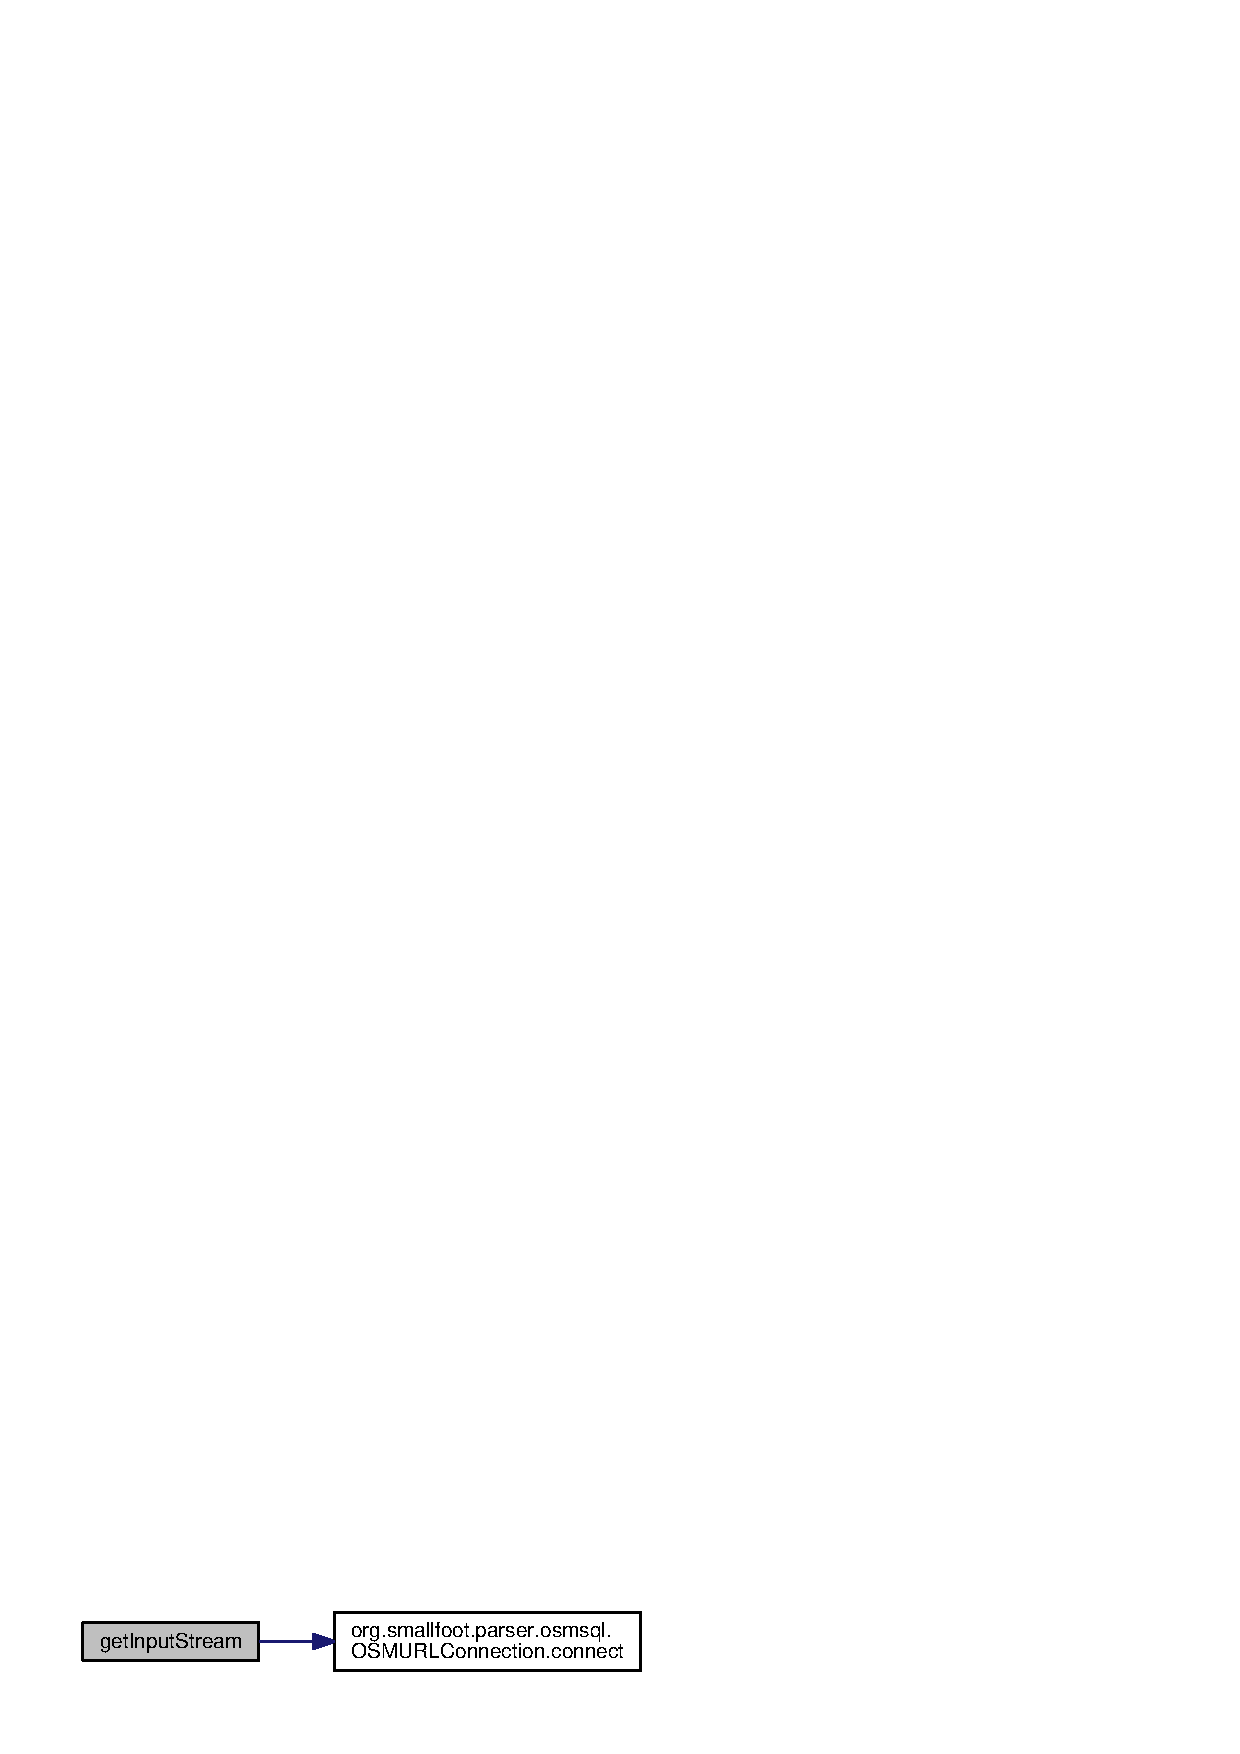
\includegraphics[width=312pt]{classorg_1_1smallfoot_1_1parser_1_1msosmsql_1_1MSDWHURLConnection_a0924d1107a459be632532ef34324494e_cgraph}
\end{center}
\end{figure}




The documentation for this class was generated from the following file\+:\begin{DoxyCompactItemize}
\item 
java/{\bf M\+S\+D\+W\+H\+U\+R\+L\+Connection.\+java}\end{DoxyCompactItemize}

\section{M\+S\+D\+W\+H\+U\+R\+L\+Connection.\+M\+S\+Result\+C\+S\+V\+Pipe Class Reference}
\label{classorg_1_1smallfoot_1_1parser_1_1msosmsql_1_1MSDWHURLConnection_1_1MSResultCSVPipe}\index{M\+S\+D\+W\+H\+U\+R\+L\+Connection.\+M\+S\+Result\+C\+S\+V\+Pipe@{M\+S\+D\+W\+H\+U\+R\+L\+Connection.\+M\+S\+Result\+C\+S\+V\+Pipe}}


Piped\+Output\+Stream to push out resultsets as C\+S\+V Nicknames.  




Inheritance diagram for M\+S\+D\+W\+H\+U\+R\+L\+Connection.\+M\+S\+Result\+C\+S\+V\+Pipe\+:\nopagebreak
\begin{figure}[H]
\begin{center}
\leavevmode
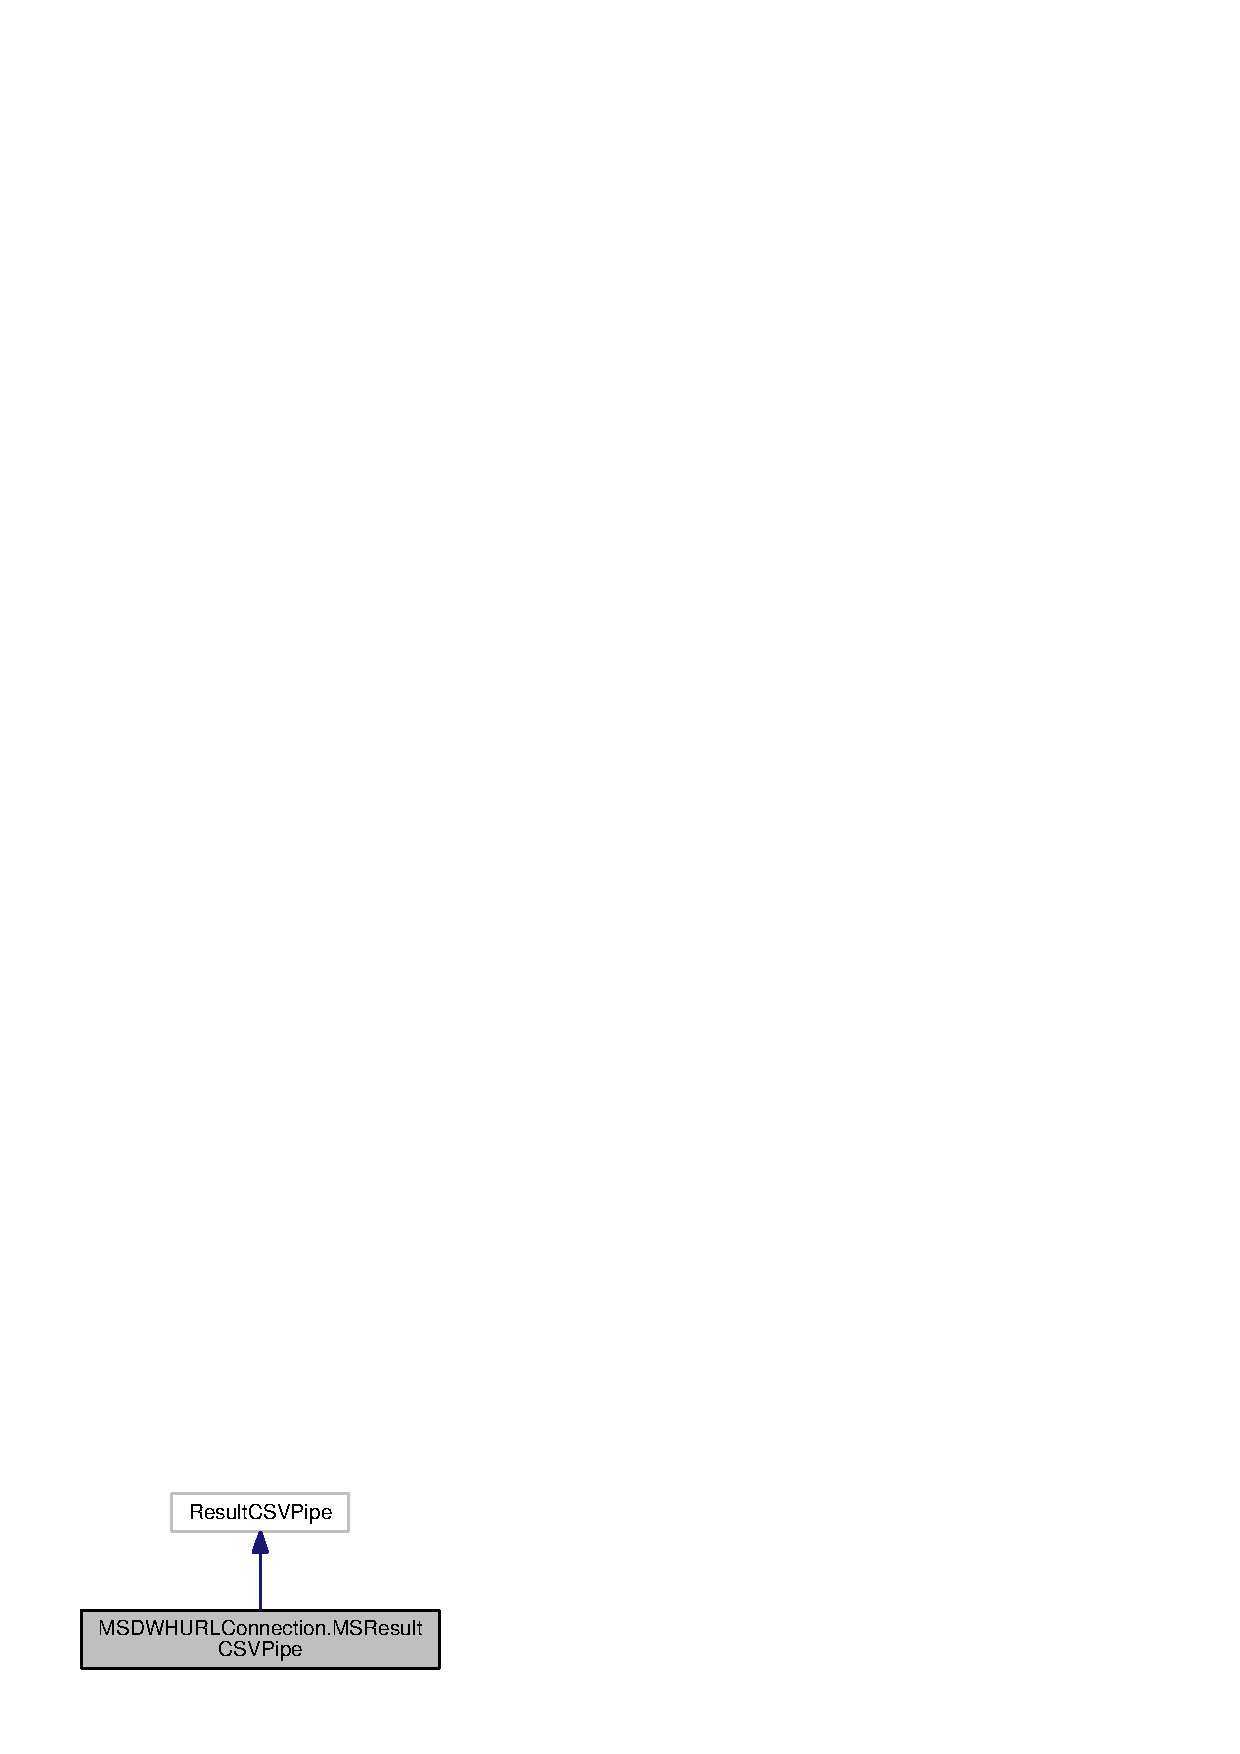
\includegraphics[width=214pt]{classorg_1_1smallfoot_1_1parser_1_1msosmsql_1_1MSDWHURLConnection_1_1MSResultCSVPipe__inherit__graph}
\end{center}
\end{figure}


Collaboration diagram for M\+S\+D\+W\+H\+U\+R\+L\+Connection.\+M\+S\+Result\+C\+S\+V\+Pipe\+:\nopagebreak
\begin{figure}[H]
\begin{center}
\leavevmode
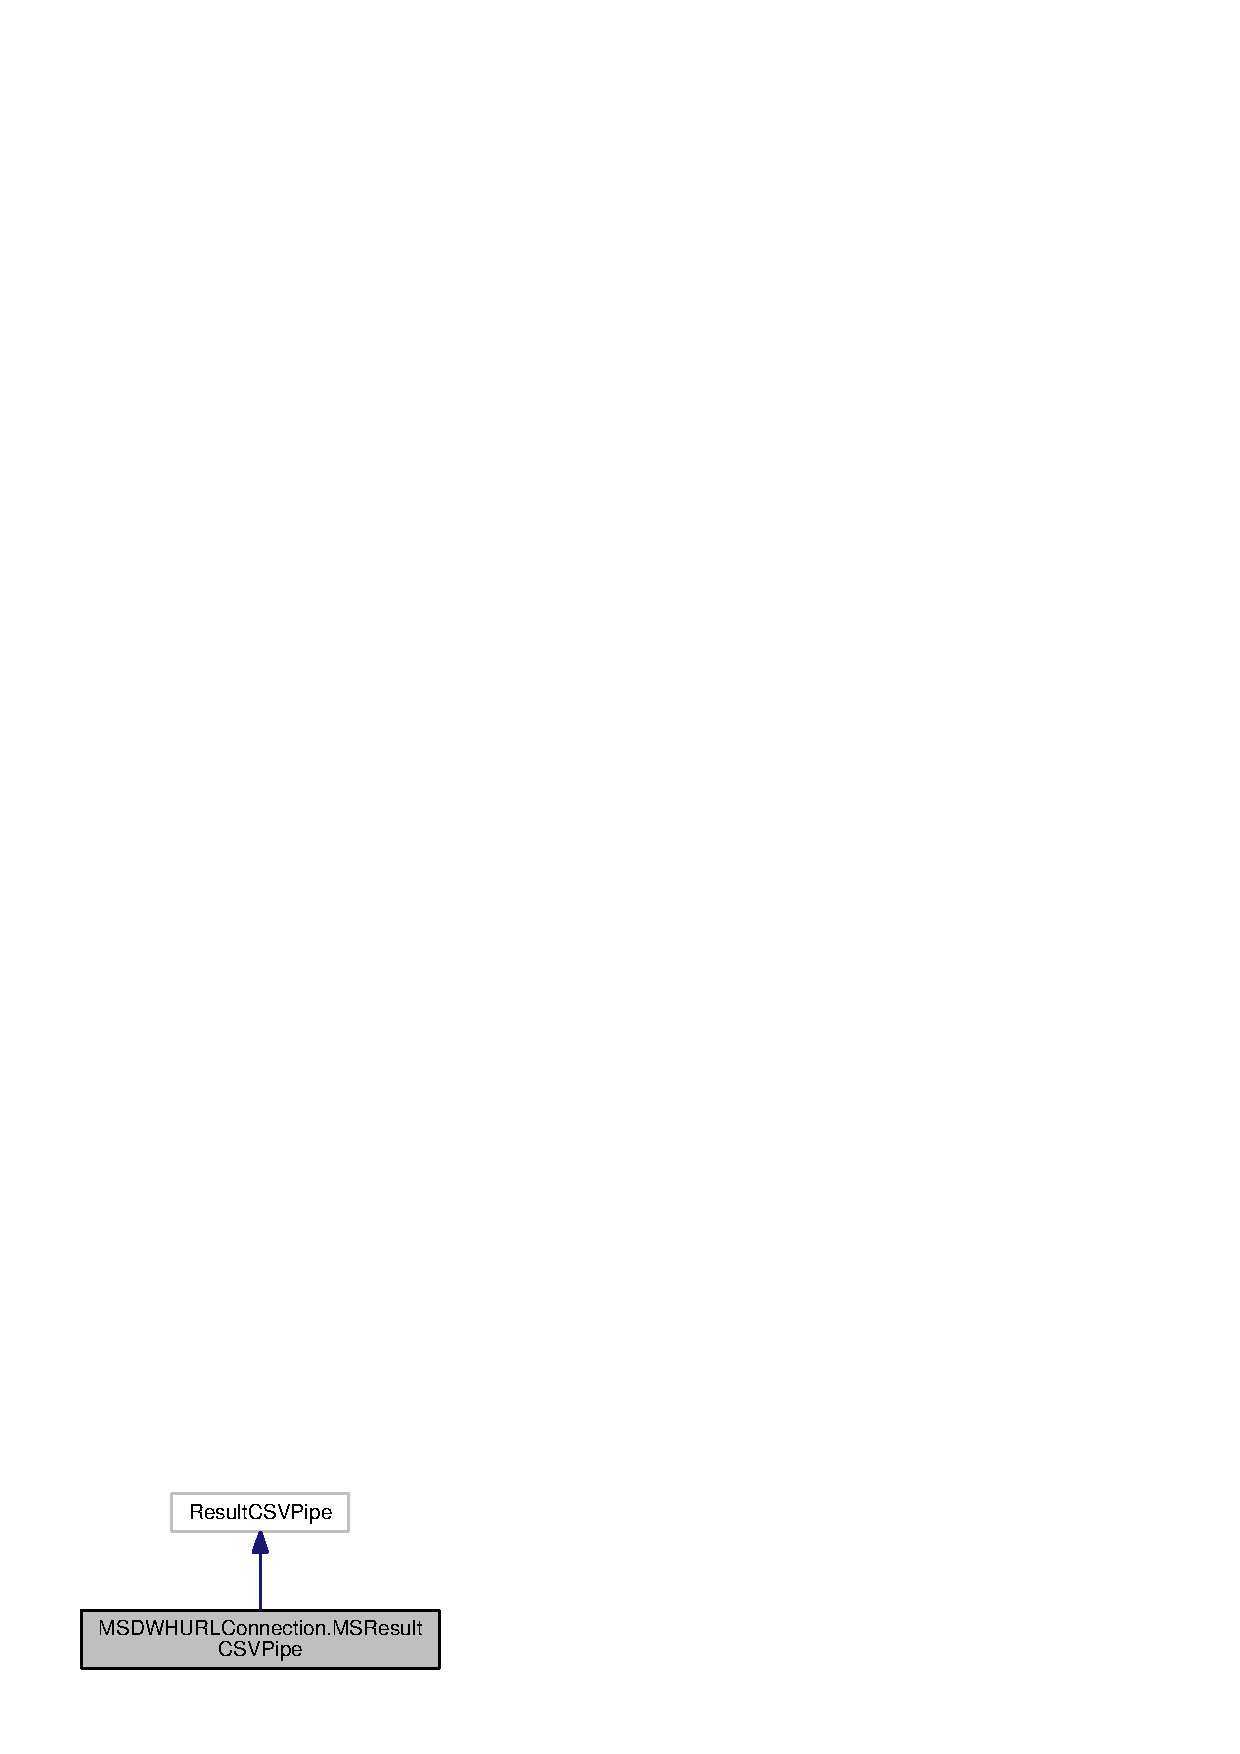
\includegraphics[width=214pt]{classorg_1_1smallfoot_1_1parser_1_1msosmsql_1_1MSDWHURLConnection_1_1MSResultCSVPipe__coll__graph}
\end{center}
\end{figure}
\subsection*{Public Member Functions}
\begin{DoxyCompactItemize}
\item 
{\bf M\+S\+Result\+C\+S\+V\+Pipe} (java.\+sql.\+Result\+Set source)
\item 
char {\bf uniqueness} (String third\+Rail)
\item 
void {\bf run} ()
\end{DoxyCompactItemize}


\subsection{Detailed Description}
Piped\+Output\+Stream to push out resultsets as C\+S\+V Nicknames. 

No, I\textquotesingle{}m not a fan of this method of doing so, I\textquotesingle{}d rather have the upstream consume data block of W\+W\+N/\+Nickname pairs, but this fits into the stream-\/reading I\textquotesingle{}ve currently got. To be shallow, it fits the current dataflow, although very soon I\textquotesingle{}m sure there will be a need to strip off the layers of hand-\/offs and go with data blocks streaming from various resources. 

Definition at line 98 of file M\+S\+D\+W\+H\+U\+R\+L\+Connection.\+java.



\subsection{Constructor \& Destructor Documentation}
\index{org\+::smallfoot\+::parser\+::msosmsql\+::\+M\+S\+D\+W\+H\+U\+R\+L\+Connection\+::\+M\+S\+Result\+C\+S\+V\+Pipe@{org\+::smallfoot\+::parser\+::msosmsql\+::\+M\+S\+D\+W\+H\+U\+R\+L\+Connection\+::\+M\+S\+Result\+C\+S\+V\+Pipe}!M\+S\+Result\+C\+S\+V\+Pipe@{M\+S\+Result\+C\+S\+V\+Pipe}}
\index{M\+S\+Result\+C\+S\+V\+Pipe@{M\+S\+Result\+C\+S\+V\+Pipe}!org\+::smallfoot\+::parser\+::msosmsql\+::\+M\+S\+D\+W\+H\+U\+R\+L\+Connection\+::\+M\+S\+Result\+C\+S\+V\+Pipe@{org\+::smallfoot\+::parser\+::msosmsql\+::\+M\+S\+D\+W\+H\+U\+R\+L\+Connection\+::\+M\+S\+Result\+C\+S\+V\+Pipe}}
\subsubsection[{M\+S\+Result\+C\+S\+V\+Pipe}]{\setlength{\rightskip}{0pt plus 5cm}{\bf M\+S\+Result\+C\+S\+V\+Pipe} (
\begin{DoxyParamCaption}
\item[{java.\+sql.\+Result\+Set}]{source}
\end{DoxyParamCaption}
)\hspace{0.3cm}{\ttfamily [inline]}}\label{classorg_1_1smallfoot_1_1parser_1_1msosmsql_1_1MSDWHURLConnection_1_1MSResultCSVPipe_a48969ca60c1736f7e57420019b30220c}


Definition at line 101 of file M\+S\+D\+W\+H\+U\+R\+L\+Connection.\+java.



\subsection{Member Function Documentation}
\index{org\+::smallfoot\+::parser\+::msosmsql\+::\+M\+S\+D\+W\+H\+U\+R\+L\+Connection\+::\+M\+S\+Result\+C\+S\+V\+Pipe@{org\+::smallfoot\+::parser\+::msosmsql\+::\+M\+S\+D\+W\+H\+U\+R\+L\+Connection\+::\+M\+S\+Result\+C\+S\+V\+Pipe}!run@{run}}
\index{run@{run}!org\+::smallfoot\+::parser\+::msosmsql\+::\+M\+S\+D\+W\+H\+U\+R\+L\+Connection\+::\+M\+S\+Result\+C\+S\+V\+Pipe@{org\+::smallfoot\+::parser\+::msosmsql\+::\+M\+S\+D\+W\+H\+U\+R\+L\+Connection\+::\+M\+S\+Result\+C\+S\+V\+Pipe}}
\subsubsection[{run}]{\setlength{\rightskip}{0pt plus 5cm}void run (
\begin{DoxyParamCaption}
{}
\end{DoxyParamCaption}
)\hspace{0.3cm}{\ttfamily [inline]}}\label{classorg_1_1smallfoot_1_1parser_1_1msosmsql_1_1MSDWHURLConnection_1_1MSResultCSVPipe_a13a43e6d814de94978c515cb084873b1}


Definition at line 125 of file M\+S\+D\+W\+H\+U\+R\+L\+Connection.\+java.



References M\+S\+D\+W\+H\+U\+R\+L\+Connection.\+M\+S\+Result\+C\+S\+V\+Pipe.\+uniqueness().



Here is the call graph for this function\+:\nopagebreak
\begin{figure}[H]
\begin{center}
\leavevmode
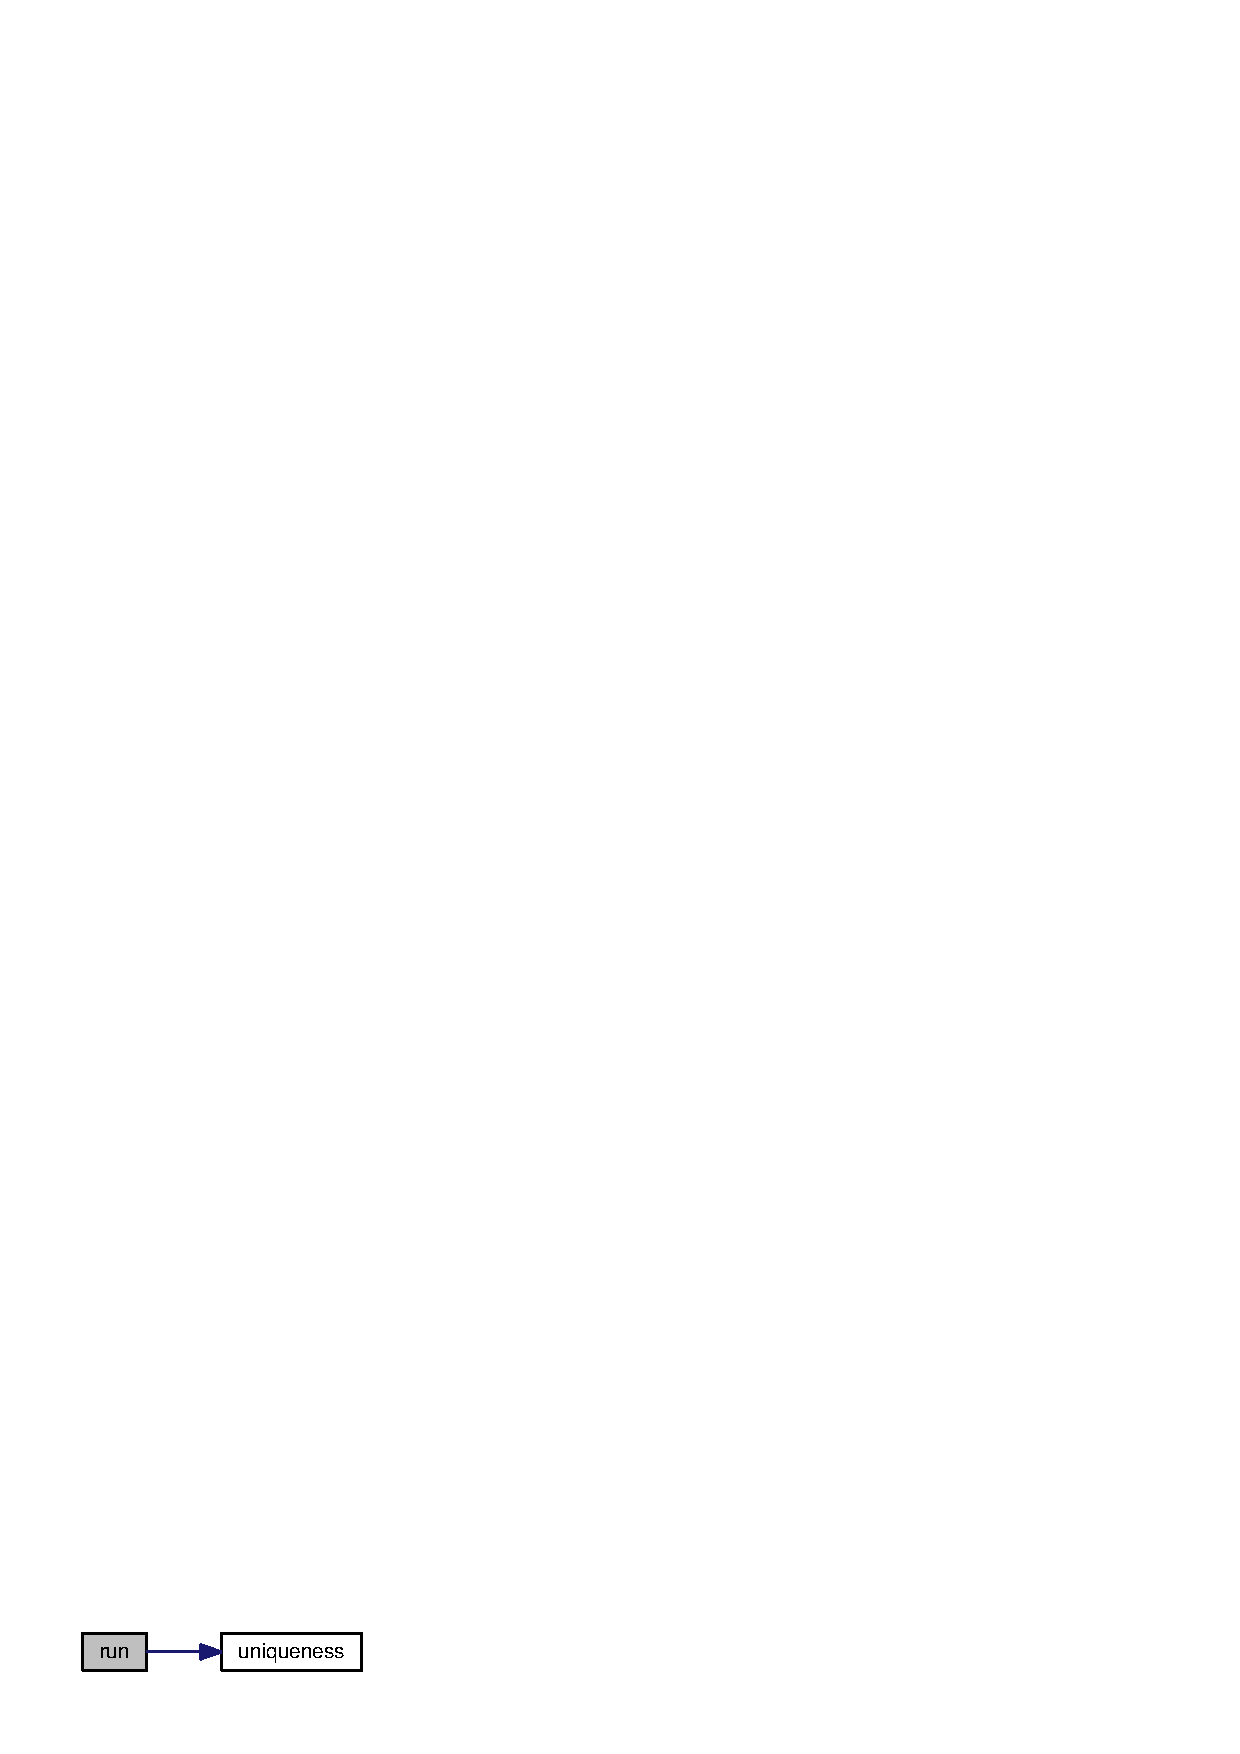
\includegraphics[width=178pt]{classorg_1_1smallfoot_1_1parser_1_1msosmsql_1_1MSDWHURLConnection_1_1MSResultCSVPipe_a13a43e6d814de94978c515cb084873b1_cgraph}
\end{center}
\end{figure}


\index{org\+::smallfoot\+::parser\+::msosmsql\+::\+M\+S\+D\+W\+H\+U\+R\+L\+Connection\+::\+M\+S\+Result\+C\+S\+V\+Pipe@{org\+::smallfoot\+::parser\+::msosmsql\+::\+M\+S\+D\+W\+H\+U\+R\+L\+Connection\+::\+M\+S\+Result\+C\+S\+V\+Pipe}!uniqueness@{uniqueness}}
\index{uniqueness@{uniqueness}!org\+::smallfoot\+::parser\+::msosmsql\+::\+M\+S\+D\+W\+H\+U\+R\+L\+Connection\+::\+M\+S\+Result\+C\+S\+V\+Pipe@{org\+::smallfoot\+::parser\+::msosmsql\+::\+M\+S\+D\+W\+H\+U\+R\+L\+Connection\+::\+M\+S\+Result\+C\+S\+V\+Pipe}}
\subsubsection[{uniqueness}]{\setlength{\rightskip}{0pt plus 5cm}char uniqueness (
\begin{DoxyParamCaption}
\item[{String}]{third\+Rail}
\end{DoxyParamCaption}
)\hspace{0.3cm}{\ttfamily [inline]}}\label{classorg_1_1smallfoot_1_1parser_1_1msosmsql_1_1MSDWHURLConnection_1_1MSResultCSVPipe_ae8fd7d31a535c027fdd2a44607614324}


Definition at line 106 of file M\+S\+D\+W\+H\+U\+R\+L\+Connection.\+java.



Referenced by M\+S\+D\+W\+H\+U\+R\+L\+Connection.\+M\+S\+Result\+C\+S\+V\+Pipe.\+run().



The documentation for this class was generated from the following file\+:\begin{DoxyCompactItemize}
\item 
java/{\bf M\+S\+D\+W\+H\+U\+R\+L\+Connection.\+java}\end{DoxyCompactItemize}

\section{Nickname\+Parser Class Reference}
\label{classorg_1_1smallfoot_1_1parser_1_1zone_1_1NicknameParser}\index{Nickname\+Parser@{Nickname\+Parser}}


Inheritance diagram for Nickname\+Parser\+:\nopagebreak
\begin{figure}[H]
\begin{center}
\leavevmode
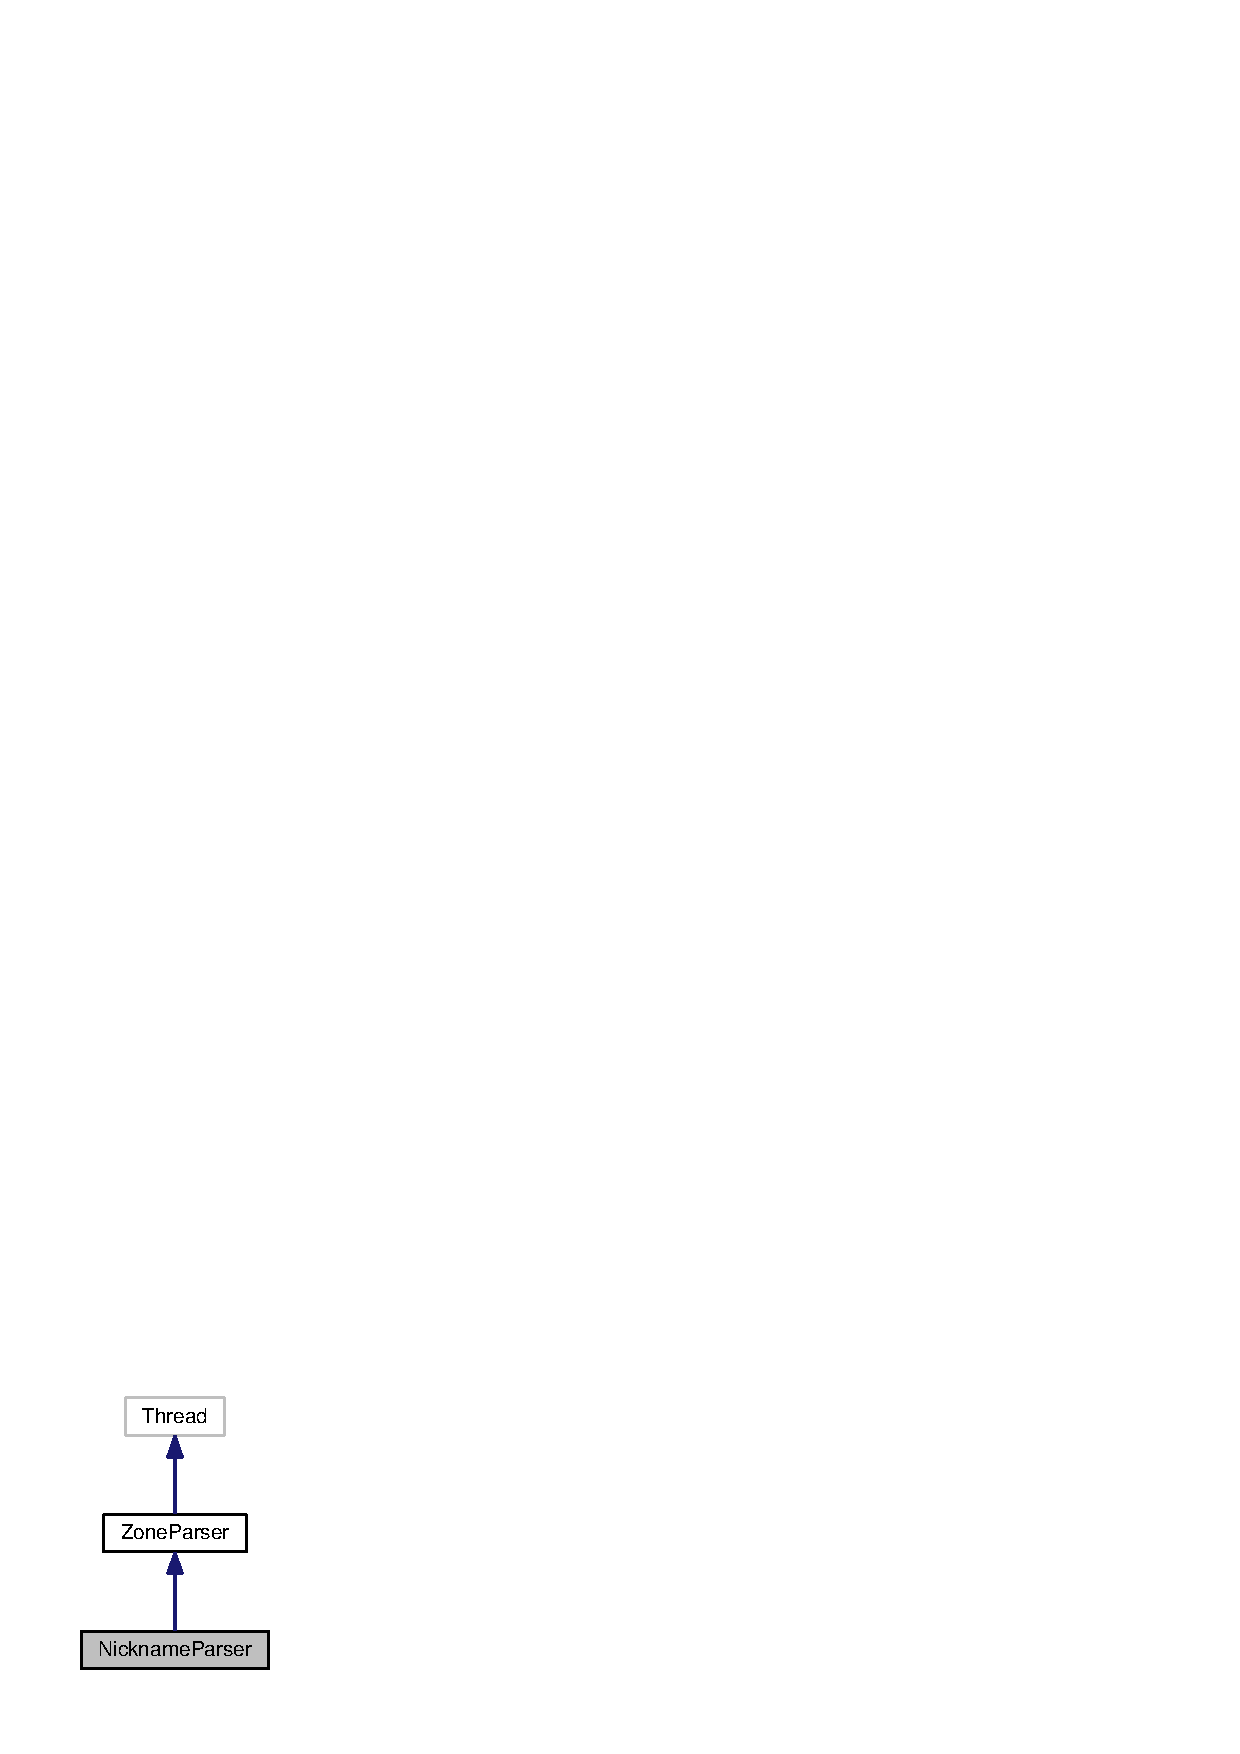
\includegraphics[width=174pt]{classorg_1_1smallfoot_1_1parser_1_1zone_1_1NicknameParser__inherit__graph}
\end{center}
\end{figure}


Collaboration diagram for Nickname\+Parser\+:\nopagebreak
\begin{figure}[H]
\begin{center}
\leavevmode
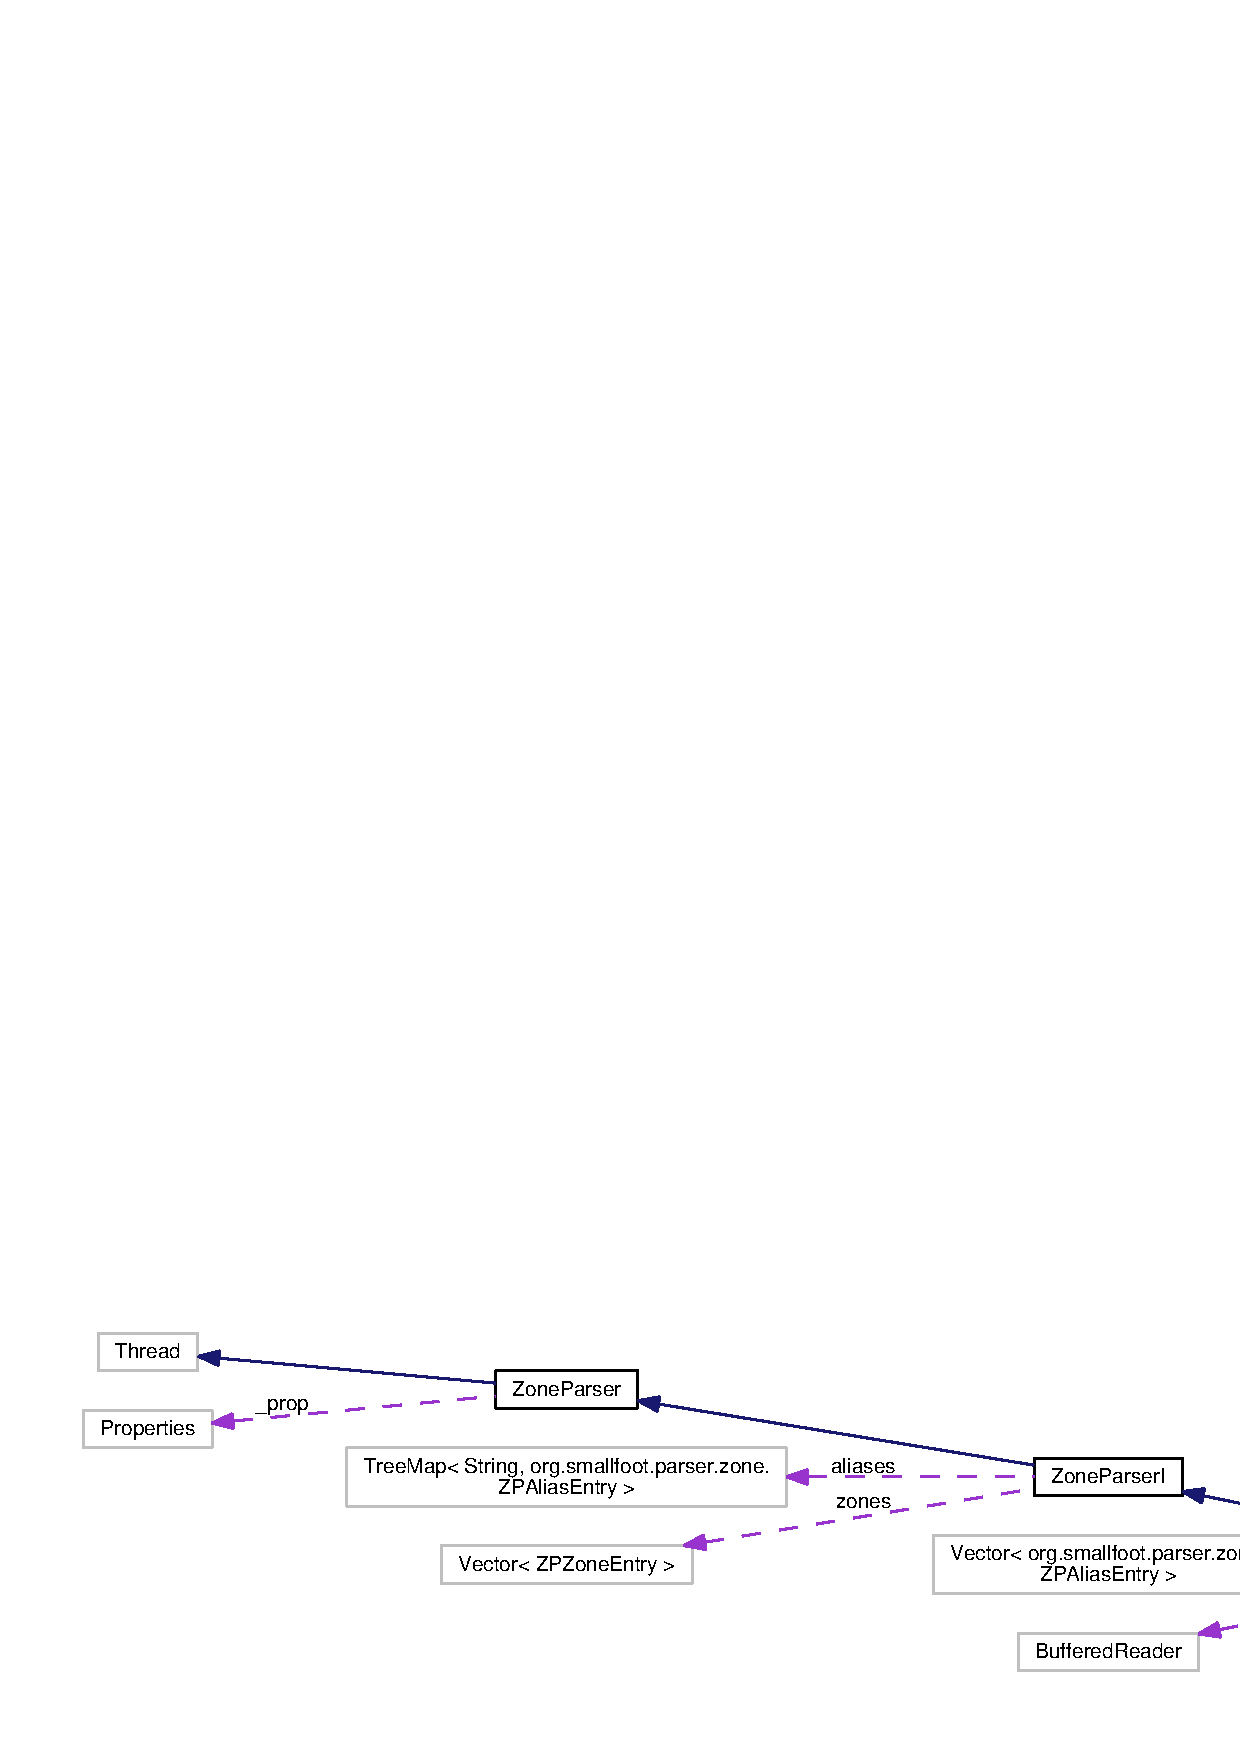
\includegraphics[width=350pt]{classorg_1_1smallfoot_1_1parser_1_1zone_1_1NicknameParser__coll__graph}
\end{center}
\end{figure}
\subsection*{Public Member Functions}
\begin{DoxyCompactItemize}
\item 
{\bf Nickname\+Parser} (java.\+util.\+Properties properties)
\begin{DoxyCompactList}\small\item\em Create a parser, setting the debug to true or false. \end{DoxyCompactList}\item 
void {\bf set\+Debug} (boolean debug)
\item 
{\bf Nickname\+Parser} (Input\+Stream in, boolean debug\+Me)
\item 
java.\+util.\+Enumeration$<$ Z\+P\+Zone\+Entry $>$ {\bf zone\+Elements} ()
\item 
int {\bf zone\+Size} ()
\item 
void {\bf set\+Reader} (java.\+io.\+Reader is)
\item 
java.\+util.\+Enumeration$<$ {\bf Z\+P\+Alias\+Entry} $>$ {\bf alias\+Elements} ()
\item 
{\bf Z\+P\+Alias\+Entry}[$\,$] {\bf alias\+Array} ()
\item 
int {\bf alias\+Size} ()
\item 
void {\bf run} ()
\end{DoxyCompactItemize}
\subsection*{Protected Member Functions}
\begin{DoxyCompactItemize}
\item 
{\bf Nickname\+Parser} (java.\+util.\+Properties properties, int col\+W\+W\+N, int col\+Nickname, boolean pedantic)
\item 
void {\bf add\+Alias} (String nick, String W\+W\+N)
\end{DoxyCompactItemize}


\subsection{Detailed Description}


Definition at line 7 of file Nickname\+Parser.\+java.



\subsection{Constructor \& Destructor Documentation}
\index{org\+::smallfoot\+::parser\+::zone\+::\+Nickname\+Parser@{org\+::smallfoot\+::parser\+::zone\+::\+Nickname\+Parser}!Nickname\+Parser@{Nickname\+Parser}}
\index{Nickname\+Parser@{Nickname\+Parser}!org\+::smallfoot\+::parser\+::zone\+::\+Nickname\+Parser@{org\+::smallfoot\+::parser\+::zone\+::\+Nickname\+Parser}}
\subsubsection[{Nickname\+Parser}]{\setlength{\rightskip}{0pt plus 5cm}{\bf Nickname\+Parser} (
\begin{DoxyParamCaption}
\item[{java.\+util.\+Properties}]{properties}
\end{DoxyParamCaption}
)\hspace{0.3cm}{\ttfamily [inline]}}\label{classorg_1_1smallfoot_1_1parser_1_1zone_1_1NicknameParser_ac7c2594b796ab3c7107f9a55b4fc8488}


Create a parser, setting the debug to true or false. 


\begin{DoxyParams}{Parameters}
{\em properties} & additional name-\/value pair collection \\
\hline
\end{DoxyParams}


Definition at line 23 of file Nickname\+Parser.\+java.

\index{org\+::smallfoot\+::parser\+::zone\+::\+Nickname\+Parser@{org\+::smallfoot\+::parser\+::zone\+::\+Nickname\+Parser}!Nickname\+Parser@{Nickname\+Parser}}
\index{Nickname\+Parser@{Nickname\+Parser}!org\+::smallfoot\+::parser\+::zone\+::\+Nickname\+Parser@{org\+::smallfoot\+::parser\+::zone\+::\+Nickname\+Parser}}
\subsubsection[{Nickname\+Parser}]{\setlength{\rightskip}{0pt plus 5cm}{\bf Nickname\+Parser} (
\begin{DoxyParamCaption}
\item[{java.\+util.\+Properties}]{properties, }
\item[{int}]{col\+W\+W\+N, }
\item[{int}]{col\+Nickname, }
\item[{boolean}]{pedantic}
\end{DoxyParamCaption}
)\hspace{0.3cm}{\ttfamily [inline]}, {\ttfamily [protected]}}\label{classorg_1_1smallfoot_1_1parser_1_1zone_1_1NicknameParser_a9541dfa4225692671d2e0b5ef0f57059}


Definition at line 34 of file Nickname\+Parser.\+java.

\index{org\+::smallfoot\+::parser\+::zone\+::\+Nickname\+Parser@{org\+::smallfoot\+::parser\+::zone\+::\+Nickname\+Parser}!Nickname\+Parser@{Nickname\+Parser}}
\index{Nickname\+Parser@{Nickname\+Parser}!org\+::smallfoot\+::parser\+::zone\+::\+Nickname\+Parser@{org\+::smallfoot\+::parser\+::zone\+::\+Nickname\+Parser}}
\subsubsection[{Nickname\+Parser}]{\setlength{\rightskip}{0pt plus 5cm}{\bf Nickname\+Parser} (
\begin{DoxyParamCaption}
\item[{Input\+Stream}]{in, }
\item[{boolean}]{debug\+Me}
\end{DoxyParamCaption}
)\hspace{0.3cm}{\ttfamily [inline]}}\label{classorg_1_1smallfoot_1_1parser_1_1zone_1_1NicknameParser_a4de85135c75bd7120150390def731fbd}


Definition at line 47 of file Nickname\+Parser.\+java.



\subsection{Member Function Documentation}
\index{org\+::smallfoot\+::parser\+::zone\+::\+Nickname\+Parser@{org\+::smallfoot\+::parser\+::zone\+::\+Nickname\+Parser}!add\+Alias@{add\+Alias}}
\index{add\+Alias@{add\+Alias}!org\+::smallfoot\+::parser\+::zone\+::\+Nickname\+Parser@{org\+::smallfoot\+::parser\+::zone\+::\+Nickname\+Parser}}
\subsubsection[{add\+Alias}]{\setlength{\rightskip}{0pt plus 5cm}void add\+Alias (
\begin{DoxyParamCaption}
\item[{String}]{nick, }
\item[{String}]{W\+W\+N}
\end{DoxyParamCaption}
)\hspace{0.3cm}{\ttfamily [inline]}, {\ttfamily [protected]}}\label{classorg_1_1smallfoot_1_1parser_1_1zone_1_1NicknameParser_a9bc4ab801fe78c7087eea21e8fcf2953}


Definition at line 84 of file Nickname\+Parser.\+java.



Referenced by Nickname\+Parser.\+run().

\index{org\+::smallfoot\+::parser\+::zone\+::\+Nickname\+Parser@{org\+::smallfoot\+::parser\+::zone\+::\+Nickname\+Parser}!alias\+Array@{alias\+Array}}
\index{alias\+Array@{alias\+Array}!org\+::smallfoot\+::parser\+::zone\+::\+Nickname\+Parser@{org\+::smallfoot\+::parser\+::zone\+::\+Nickname\+Parser}}
\subsubsection[{alias\+Array}]{\setlength{\rightskip}{0pt plus 5cm}{\bf Z\+P\+Alias\+Entry} [$\,$] alias\+Array (
\begin{DoxyParamCaption}
{}
\end{DoxyParamCaption}
)\hspace{0.3cm}{\ttfamily [inline]}}\label{classorg_1_1smallfoot_1_1parser_1_1zone_1_1NicknameParser_a5c646608669073b5c31bb44626baa48f}


Definition at line 73 of file Nickname\+Parser.\+java.

\index{org\+::smallfoot\+::parser\+::zone\+::\+Nickname\+Parser@{org\+::smallfoot\+::parser\+::zone\+::\+Nickname\+Parser}!alias\+Elements@{alias\+Elements}}
\index{alias\+Elements@{alias\+Elements}!org\+::smallfoot\+::parser\+::zone\+::\+Nickname\+Parser@{org\+::smallfoot\+::parser\+::zone\+::\+Nickname\+Parser}}
\subsubsection[{alias\+Elements}]{\setlength{\rightskip}{0pt plus 5cm}java.\+util.\+Enumeration$<${\bf Z\+P\+Alias\+Entry}$>$ alias\+Elements (
\begin{DoxyParamCaption}
{}
\end{DoxyParamCaption}
)\hspace{0.3cm}{\ttfamily [inline]}}\label{classorg_1_1smallfoot_1_1parser_1_1zone_1_1NicknameParser_a1631138fd08af051dc26686c00768ab3}


Definition at line 67 of file Nickname\+Parser.\+java.

\index{org\+::smallfoot\+::parser\+::zone\+::\+Nickname\+Parser@{org\+::smallfoot\+::parser\+::zone\+::\+Nickname\+Parser}!alias\+Size@{alias\+Size}}
\index{alias\+Size@{alias\+Size}!org\+::smallfoot\+::parser\+::zone\+::\+Nickname\+Parser@{org\+::smallfoot\+::parser\+::zone\+::\+Nickname\+Parser}}
\subsubsection[{alias\+Size}]{\setlength{\rightskip}{0pt plus 5cm}int alias\+Size (
\begin{DoxyParamCaption}
{}
\end{DoxyParamCaption}
)\hspace{0.3cm}{\ttfamily [inline]}}\label{classorg_1_1smallfoot_1_1parser_1_1zone_1_1NicknameParser_a5586367d58e0d7e6a4d5262d6dc87fd2}


Definition at line 78 of file Nickname\+Parser.\+java.

\index{org\+::smallfoot\+::parser\+::zone\+::\+Nickname\+Parser@{org\+::smallfoot\+::parser\+::zone\+::\+Nickname\+Parser}!run@{run}}
\index{run@{run}!org\+::smallfoot\+::parser\+::zone\+::\+Nickname\+Parser@{org\+::smallfoot\+::parser\+::zone\+::\+Nickname\+Parser}}
\subsubsection[{run}]{\setlength{\rightskip}{0pt plus 5cm}void run (
\begin{DoxyParamCaption}
{}
\end{DoxyParamCaption}
)\hspace{0.3cm}{\ttfamily [inline]}}\label{classorg_1_1smallfoot_1_1parser_1_1zone_1_1NicknameParser_a13a43e6d814de94978c515cb084873b1}


Definition at line 91 of file Nickname\+Parser.\+java.



References Nickname\+Parser.\+add\+Alias().



Here is the call graph for this function\+:\nopagebreak
\begin{figure}[H]
\begin{center}
\leavevmode
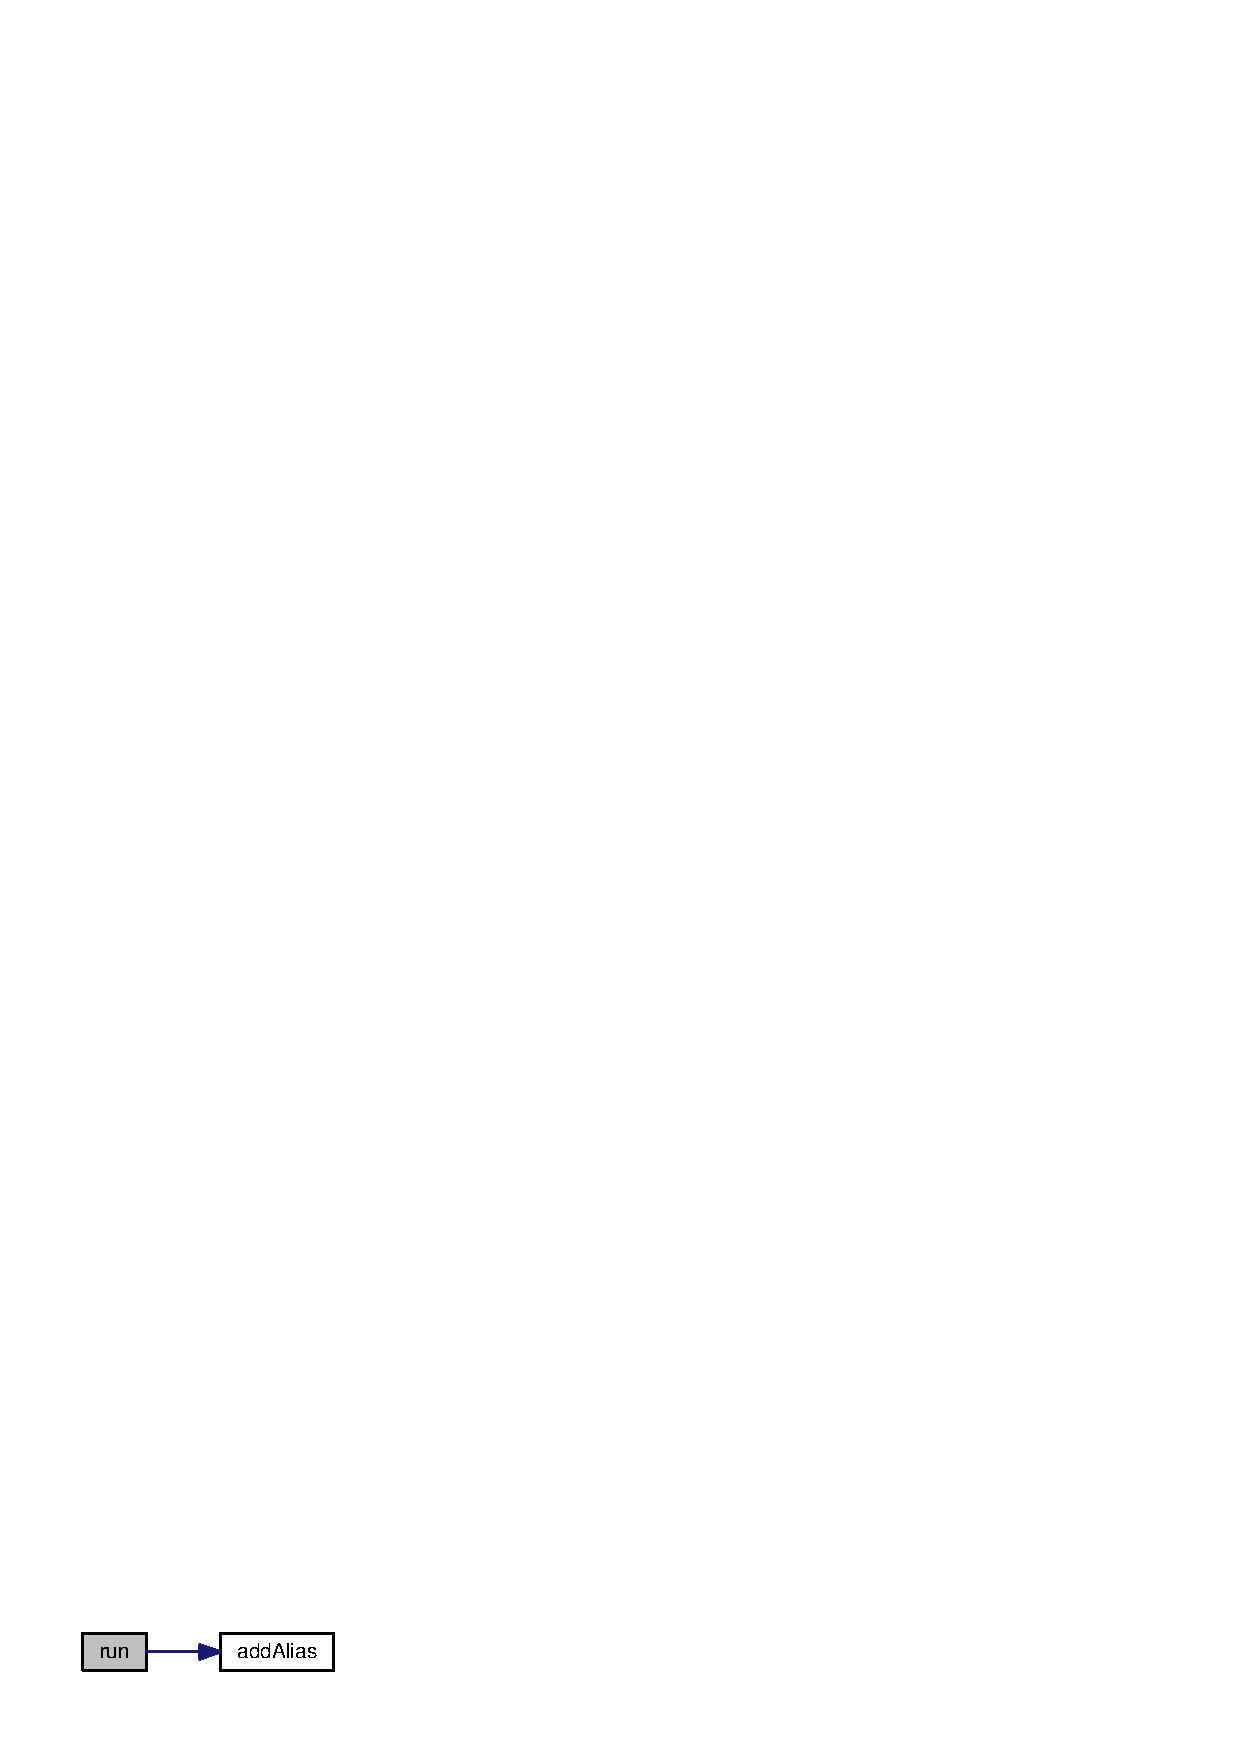
\includegraphics[width=164pt]{classorg_1_1smallfoot_1_1parser_1_1zone_1_1NicknameParser_a13a43e6d814de94978c515cb084873b1_cgraph}
\end{center}
\end{figure}


\index{org\+::smallfoot\+::parser\+::zone\+::\+Nickname\+Parser@{org\+::smallfoot\+::parser\+::zone\+::\+Nickname\+Parser}!set\+Debug@{set\+Debug}}
\index{set\+Debug@{set\+Debug}!org\+::smallfoot\+::parser\+::zone\+::\+Nickname\+Parser@{org\+::smallfoot\+::parser\+::zone\+::\+Nickname\+Parser}}
\subsubsection[{set\+Debug}]{\setlength{\rightskip}{0pt plus 5cm}void set\+Debug (
\begin{DoxyParamCaption}
\item[{boolean}]{debug}
\end{DoxyParamCaption}
)\hspace{0.3cm}{\ttfamily [inline]}}\label{classorg_1_1smallfoot_1_1parser_1_1zone_1_1NicknameParser_a6c13d260cf71d0554f789c4641a9f18b}


Definition at line 43 of file Nickname\+Parser.\+java.

\index{org\+::smallfoot\+::parser\+::zone\+::\+Nickname\+Parser@{org\+::smallfoot\+::parser\+::zone\+::\+Nickname\+Parser}!set\+Reader@{set\+Reader}}
\index{set\+Reader@{set\+Reader}!org\+::smallfoot\+::parser\+::zone\+::\+Nickname\+Parser@{org\+::smallfoot\+::parser\+::zone\+::\+Nickname\+Parser}}
\subsubsection[{set\+Reader}]{\setlength{\rightskip}{0pt plus 5cm}void set\+Reader (
\begin{DoxyParamCaption}
\item[{java.\+io.\+Reader}]{is}
\end{DoxyParamCaption}
)\hspace{0.3cm}{\ttfamily [inline]}}\label{classorg_1_1smallfoot_1_1parser_1_1zone_1_1NicknameParser_aa89f56e94a76b211df071f905e7288ae}


Definition at line 62 of file Nickname\+Parser.\+java.

\index{org\+::smallfoot\+::parser\+::zone\+::\+Nickname\+Parser@{org\+::smallfoot\+::parser\+::zone\+::\+Nickname\+Parser}!zone\+Elements@{zone\+Elements}}
\index{zone\+Elements@{zone\+Elements}!org\+::smallfoot\+::parser\+::zone\+::\+Nickname\+Parser@{org\+::smallfoot\+::parser\+::zone\+::\+Nickname\+Parser}}
\subsubsection[{zone\+Elements}]{\setlength{\rightskip}{0pt plus 5cm}java.\+util.\+Enumeration$<$Z\+P\+Zone\+Entry$>$ zone\+Elements (
\begin{DoxyParamCaption}
{}
\end{DoxyParamCaption}
)\hspace{0.3cm}{\ttfamily [inline]}}\label{classorg_1_1smallfoot_1_1parser_1_1zone_1_1NicknameParser_a17bb9b86877d4493c7ad4ba284f7c945}


Definition at line 52 of file Nickname\+Parser.\+java.

\index{org\+::smallfoot\+::parser\+::zone\+::\+Nickname\+Parser@{org\+::smallfoot\+::parser\+::zone\+::\+Nickname\+Parser}!zone\+Size@{zone\+Size}}
\index{zone\+Size@{zone\+Size}!org\+::smallfoot\+::parser\+::zone\+::\+Nickname\+Parser@{org\+::smallfoot\+::parser\+::zone\+::\+Nickname\+Parser}}
\subsubsection[{zone\+Size}]{\setlength{\rightskip}{0pt plus 5cm}int zone\+Size (
\begin{DoxyParamCaption}
{}
\end{DoxyParamCaption}
)\hspace{0.3cm}{\ttfamily [inline]}}\label{classorg_1_1smallfoot_1_1parser_1_1zone_1_1NicknameParser_a083293963a3e77da41becf829be83aca}


Definition at line 57 of file Nickname\+Parser.\+java.



The documentation for this class was generated from the following file\+:\begin{DoxyCompactItemize}
\item 
java/{\bf Nickname\+Parser.\+java}\end{DoxyCompactItemize}

\section{O\+S\+M\+U\+R\+L\+Connection Class Reference}
\label{classorg_1_1smallfoot_1_1parser_1_1osmsql_1_1OSMURLConnection}\index{O\+S\+M\+U\+R\+L\+Connection@{O\+S\+M\+U\+R\+L\+Connection}}


Inheritance diagram for O\+S\+M\+U\+R\+L\+Connection\+:\nopagebreak
\begin{figure}[H]
\begin{center}
\leavevmode
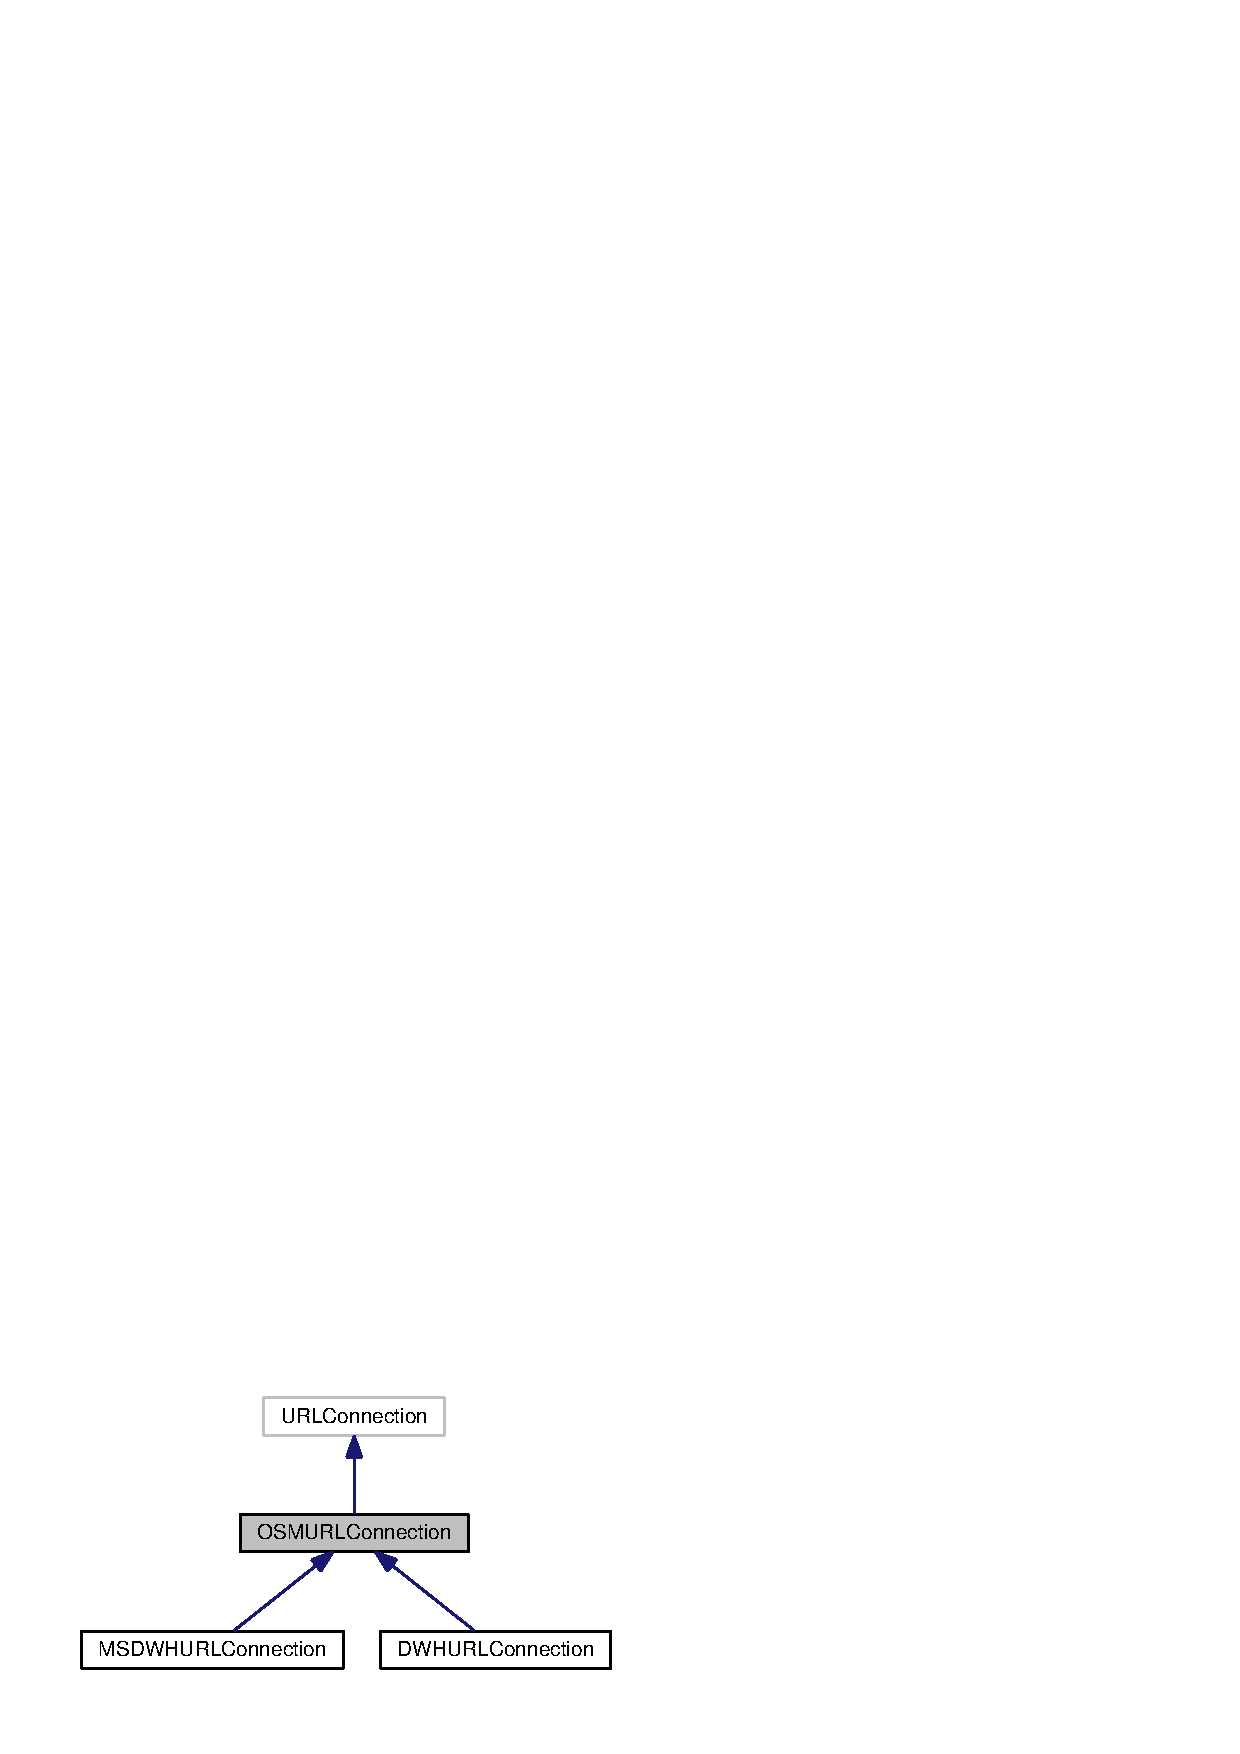
\includegraphics[width=297pt]{classorg_1_1smallfoot_1_1parser_1_1osmsql_1_1OSMURLConnection__inherit__graph}
\end{center}
\end{figure}


Collaboration diagram for O\+S\+M\+U\+R\+L\+Connection\+:\nopagebreak
\begin{figure}[H]
\begin{center}
\leavevmode
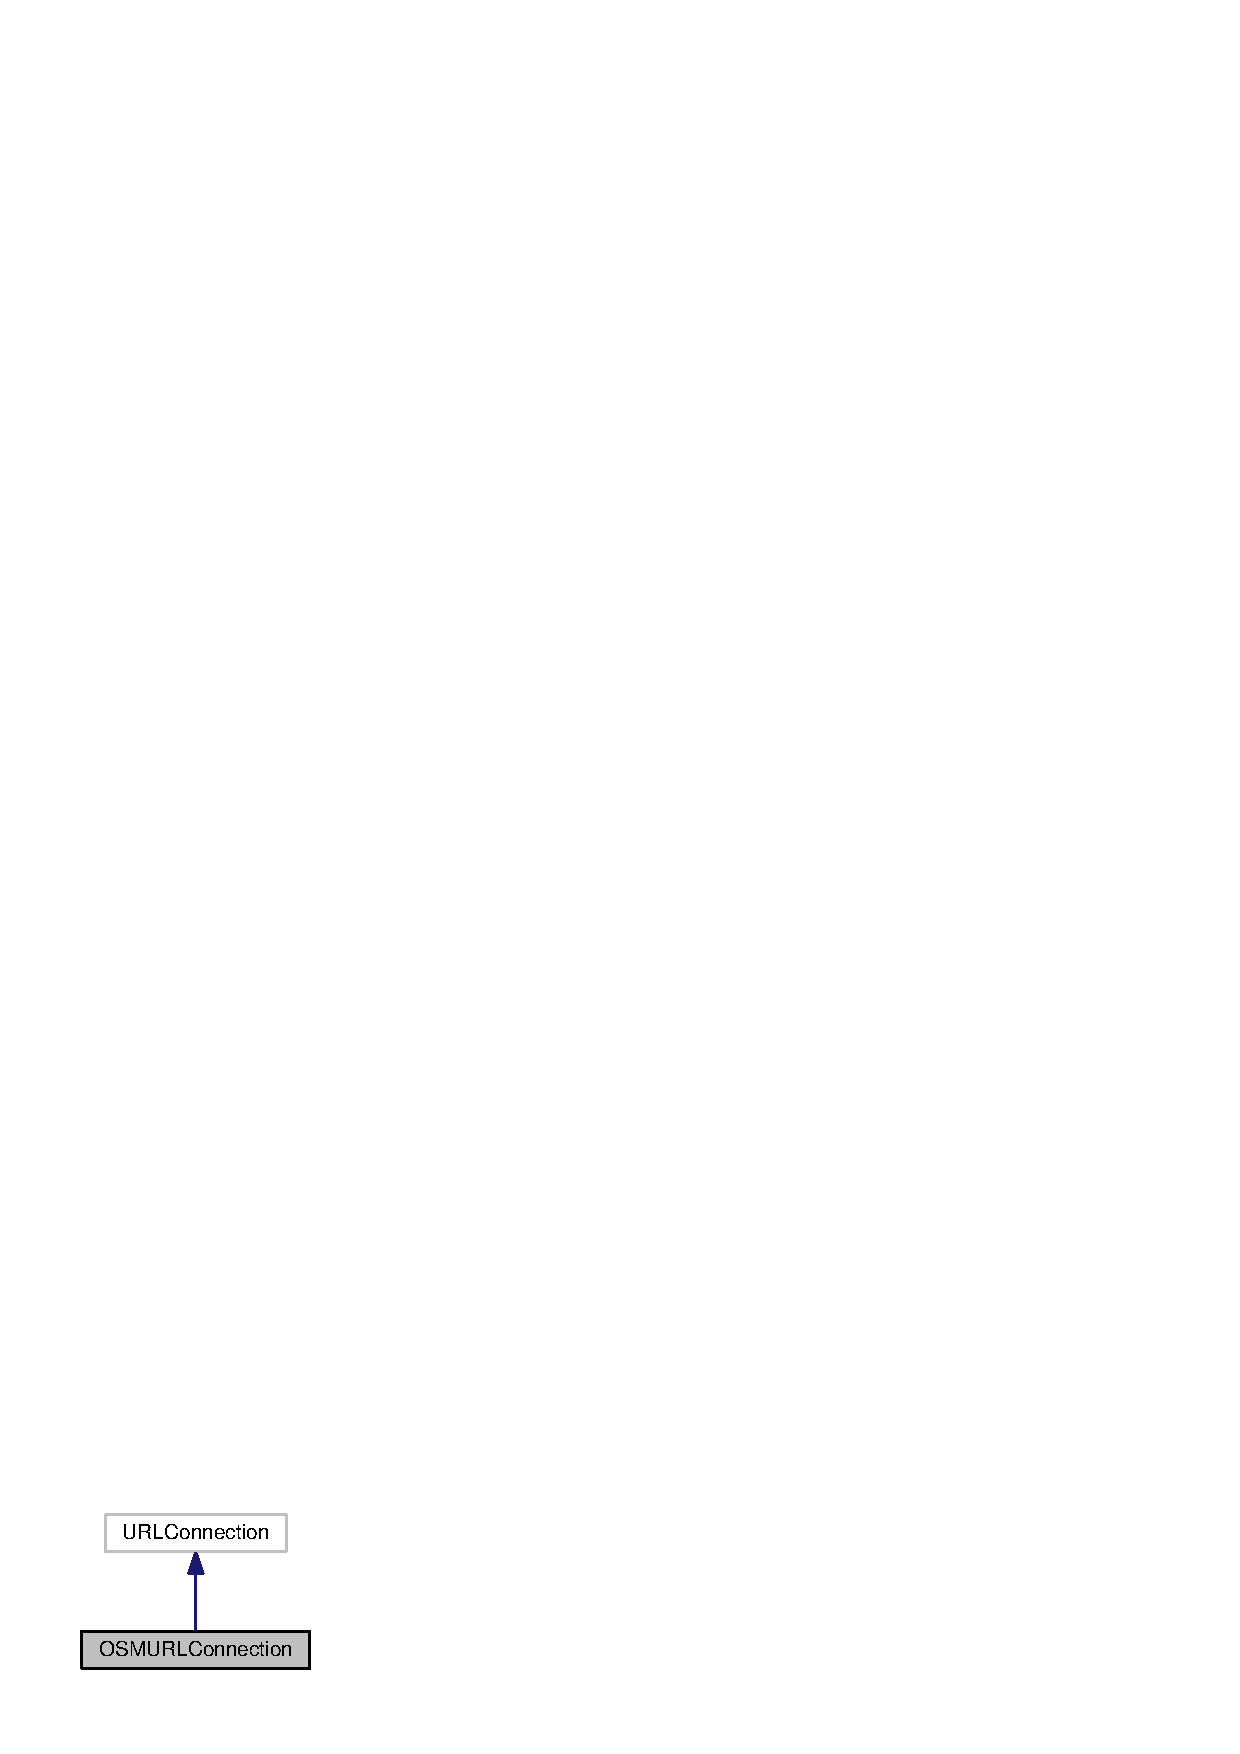
\includegraphics[width=152pt]{classorg_1_1smallfoot_1_1parser_1_1osmsql_1_1OSMURLConnection__coll__graph}
\end{center}
\end{figure}
\subsection*{Data Structures}
\begin{DoxyCompactItemize}
\item 
class {\bf Result\+C\+S\+V\+Pipe}
\begin{DoxyCompactList}\small\item\em Piped\+Output\+Stream to push out resultsets as C\+S\+V Nicknames. \end{DoxyCompactList}\end{DoxyCompactItemize}
\subsection*{Public Member Functions}
\begin{DoxyCompactItemize}
\item 
{\bf O\+S\+M\+U\+R\+L\+Connection} (String connection\+Info, String username, String password)
\item 
{\bf O\+S\+M\+U\+R\+L\+Connection} (java.\+net.\+U\+R\+L url)
\item 
void {\bf set\+Request\+Header} (String name, String value)
\begin{DoxyCompactList}\small\item\em Stubbed, because there's no change we want to accept yet. \end{DoxyCompactList}\item 
void {\bf set\+Content\+Type} (String ignored)
\begin{DoxyCompactList}\small\item\em Stubbed, because there's no change we want to accept yet. \end{DoxyCompactList}\item 
java.\+io.\+Output\+Stream {\bf get\+Output\+Stream} ()
\begin{DoxyCompactList}\small\item\em Stubbed, because there's nothing to send us. \end{DoxyCompactList}\item 
java.\+io.\+Input\+Stream {\bf get\+Input\+Stream} ()
\begin{DoxyCompactList}\small\item\em connect the result of a \char`\"{}\+S\+E\+L\+E\+C\+T hp.\+wwn, h.\+name F\+R\+O\+M host\+\_\+port hp J\+O\+I\+N host h O\+N (h.\+id = hp.\+hostid)\char`\"{} to something that looks readable like an Input\+Stream \end{DoxyCompactList}\item 
void {\bf connect} ()
\end{DoxyCompactItemize}
\subsection*{Protected Member Functions}
\begin{DoxyCompactItemize}
\item 
{\bf O\+S\+M\+U\+R\+L\+Connection} {\bf open\+Connection} (java.\+net.\+U\+R\+L url)
\begin{DoxyCompactList}\small\item\em open\+Connection(java.\+net.\+U\+R\+L) overrides java.\+net.\+U\+R\+L\+Stream\+Handler.\+open\+Connection(\+U\+R\+L) by wrapping a pgsql client. \end{DoxyCompactList}\end{DoxyCompactItemize}
\subsection*{Protected Attributes}
\begin{DoxyCompactItemize}
\item 
java.\+sql.\+Connection {\bf connection}
\end{DoxyCompactItemize}


\subsection{Detailed Description}


Definition at line 32 of file O\+S\+M\+U\+R\+L\+Connection.\+java.



\subsection{Constructor \& Destructor Documentation}
\index{org\+::smallfoot\+::parser\+::osmsql\+::\+O\+S\+M\+U\+R\+L\+Connection@{org\+::smallfoot\+::parser\+::osmsql\+::\+O\+S\+M\+U\+R\+L\+Connection}!O\+S\+M\+U\+R\+L\+Connection@{O\+S\+M\+U\+R\+L\+Connection}}
\index{O\+S\+M\+U\+R\+L\+Connection@{O\+S\+M\+U\+R\+L\+Connection}!org\+::smallfoot\+::parser\+::osmsql\+::\+O\+S\+M\+U\+R\+L\+Connection@{org\+::smallfoot\+::parser\+::osmsql\+::\+O\+S\+M\+U\+R\+L\+Connection}}
\subsubsection[{O\+S\+M\+U\+R\+L\+Connection}]{\setlength{\rightskip}{0pt plus 5cm}{\bf O\+S\+M\+U\+R\+L\+Connection} (
\begin{DoxyParamCaption}
\item[{String}]{connection\+Info, }
\item[{String}]{username, }
\item[{String}]{password}
\end{DoxyParamCaption}
)\hspace{0.3cm}{\ttfamily [inline]}}\label{classorg_1_1smallfoot_1_1parser_1_1osmsql_1_1OSMURLConnection_a8d24fe354da1d971ba65c3919942c0a8}


Definition at line 94 of file O\+S\+M\+U\+R\+L\+Connection.\+java.

\index{org\+::smallfoot\+::parser\+::osmsql\+::\+O\+S\+M\+U\+R\+L\+Connection@{org\+::smallfoot\+::parser\+::osmsql\+::\+O\+S\+M\+U\+R\+L\+Connection}!O\+S\+M\+U\+R\+L\+Connection@{O\+S\+M\+U\+R\+L\+Connection}}
\index{O\+S\+M\+U\+R\+L\+Connection@{O\+S\+M\+U\+R\+L\+Connection}!org\+::smallfoot\+::parser\+::osmsql\+::\+O\+S\+M\+U\+R\+L\+Connection@{org\+::smallfoot\+::parser\+::osmsql\+::\+O\+S\+M\+U\+R\+L\+Connection}}
\subsubsection[{O\+S\+M\+U\+R\+L\+Connection}]{\setlength{\rightskip}{0pt plus 5cm}{\bf O\+S\+M\+U\+R\+L\+Connection} (
\begin{DoxyParamCaption}
\item[{java.\+net.\+U\+R\+L}]{url}
\end{DoxyParamCaption}
)\hspace{0.3cm}{\ttfamily [inline]}}\label{classorg_1_1smallfoot_1_1parser_1_1osmsql_1_1OSMURLConnection_a463b0498cc546b8e181b4c9abc80ef91}


Definition at line 103 of file O\+S\+M\+U\+R\+L\+Connection.\+java.



\subsection{Member Function Documentation}
\index{org\+::smallfoot\+::parser\+::osmsql\+::\+O\+S\+M\+U\+R\+L\+Connection@{org\+::smallfoot\+::parser\+::osmsql\+::\+O\+S\+M\+U\+R\+L\+Connection}!connect@{connect}}
\index{connect@{connect}!org\+::smallfoot\+::parser\+::osmsql\+::\+O\+S\+M\+U\+R\+L\+Connection@{org\+::smallfoot\+::parser\+::osmsql\+::\+O\+S\+M\+U\+R\+L\+Connection}}
\subsubsection[{connect}]{\setlength{\rightskip}{0pt plus 5cm}void connect (
\begin{DoxyParamCaption}
{}
\end{DoxyParamCaption}
)\hspace{0.3cm}{\ttfamily [inline]}}\label{classorg_1_1smallfoot_1_1parser_1_1osmsql_1_1OSMURLConnection_a1396bf9b5defe9fa844a63b5cd40ac0e}


Definition at line 216 of file O\+S\+M\+U\+R\+L\+Connection.\+java.



References O\+S\+M\+U\+R\+L\+Connection.\+connection.



Referenced by M\+S\+D\+W\+H\+U\+R\+L\+Connection.\+get\+Input\+Stream(), and O\+S\+M\+U\+R\+L\+Connection.\+get\+Input\+Stream().

\index{org\+::smallfoot\+::parser\+::osmsql\+::\+O\+S\+M\+U\+R\+L\+Connection@{org\+::smallfoot\+::parser\+::osmsql\+::\+O\+S\+M\+U\+R\+L\+Connection}!get\+Input\+Stream@{get\+Input\+Stream}}
\index{get\+Input\+Stream@{get\+Input\+Stream}!org\+::smallfoot\+::parser\+::osmsql\+::\+O\+S\+M\+U\+R\+L\+Connection@{org\+::smallfoot\+::parser\+::osmsql\+::\+O\+S\+M\+U\+R\+L\+Connection}}
\subsubsection[{get\+Input\+Stream}]{\setlength{\rightskip}{0pt plus 5cm}java.\+io.\+Input\+Stream get\+Input\+Stream (
\begin{DoxyParamCaption}
{}
\end{DoxyParamCaption}
)\hspace{0.3cm}{\ttfamily [inline]}}\label{classorg_1_1smallfoot_1_1parser_1_1osmsql_1_1OSMURLConnection_a0924d1107a459be632532ef34324494e}


connect the result of a \char`\"{}\+S\+E\+L\+E\+C\+T hp.\+wwn, h.\+name F\+R\+O\+M host\+\_\+port hp J\+O\+I\+N host h O\+N (h.\+id = hp.\+hostid)\char`\"{} to something that looks readable like an Input\+Stream 



Definition at line 167 of file O\+S\+M\+U\+R\+L\+Connection.\+java.



References O\+S\+M\+U\+R\+L\+Connection.\+connect(), and O\+S\+M\+U\+R\+L\+Connection.\+connection.



Here is the call graph for this function\+:\nopagebreak
\begin{figure}[H]
\begin{center}
\leavevmode
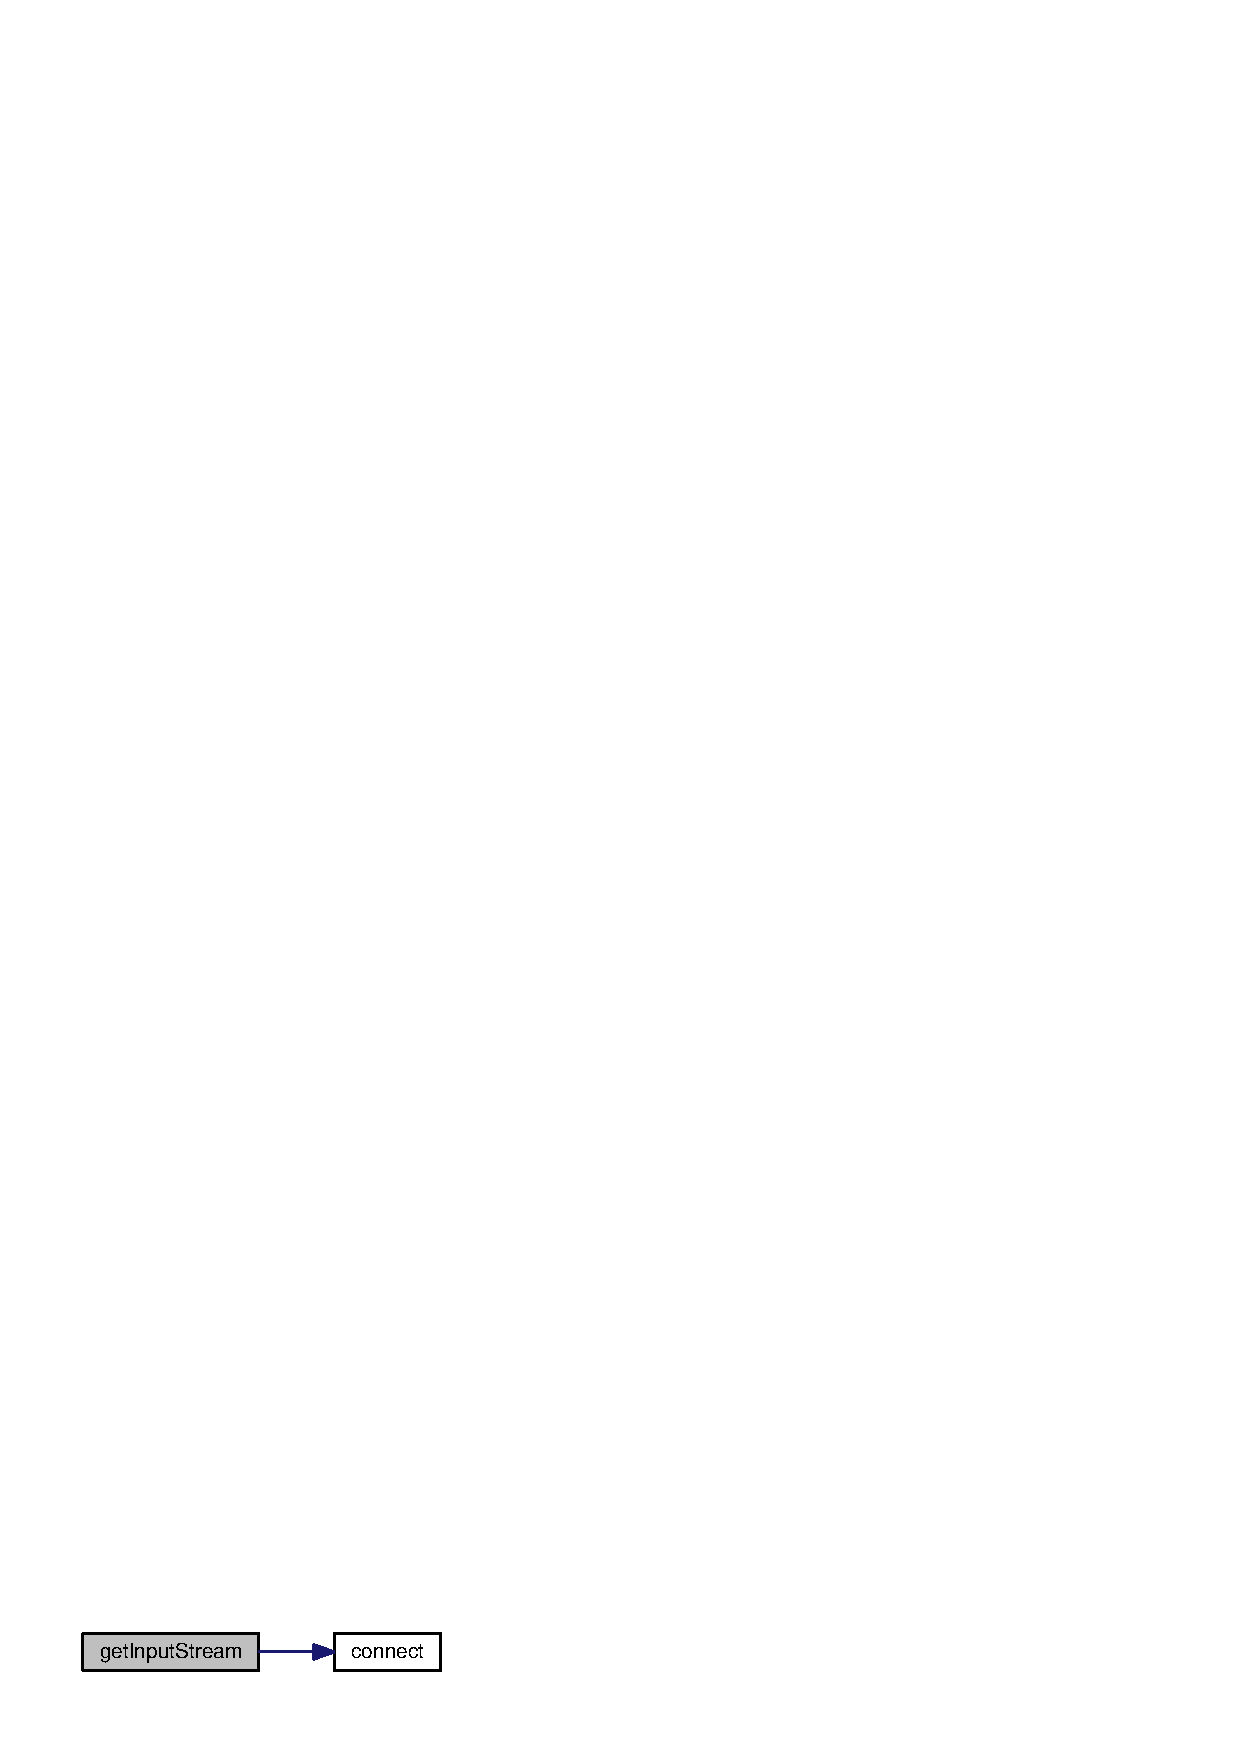
\includegraphics[width=216pt]{classorg_1_1smallfoot_1_1parser_1_1osmsql_1_1OSMURLConnection_a0924d1107a459be632532ef34324494e_cgraph}
\end{center}
\end{figure}


\index{org\+::smallfoot\+::parser\+::osmsql\+::\+O\+S\+M\+U\+R\+L\+Connection@{org\+::smallfoot\+::parser\+::osmsql\+::\+O\+S\+M\+U\+R\+L\+Connection}!get\+Output\+Stream@{get\+Output\+Stream}}
\index{get\+Output\+Stream@{get\+Output\+Stream}!org\+::smallfoot\+::parser\+::osmsql\+::\+O\+S\+M\+U\+R\+L\+Connection@{org\+::smallfoot\+::parser\+::osmsql\+::\+O\+S\+M\+U\+R\+L\+Connection}}
\subsubsection[{get\+Output\+Stream}]{\setlength{\rightskip}{0pt plus 5cm}java.\+io.\+Output\+Stream get\+Output\+Stream (
\begin{DoxyParamCaption}
{}
\end{DoxyParamCaption}
)\hspace{0.3cm}{\ttfamily [inline]}}\label{classorg_1_1smallfoot_1_1parser_1_1osmsql_1_1OSMURLConnection_a4170f42681efaf92df5c2030f5298905}


Stubbed, because there's nothing to send us. 

Oh how did I get caught in the \char`\"{}\+Royal '\+We'\char`\"{} ? 

Definition at line 158 of file O\+S\+M\+U\+R\+L\+Connection.\+java.

\index{org\+::smallfoot\+::parser\+::osmsql\+::\+O\+S\+M\+U\+R\+L\+Connection@{org\+::smallfoot\+::parser\+::osmsql\+::\+O\+S\+M\+U\+R\+L\+Connection}!open\+Connection@{open\+Connection}}
\index{open\+Connection@{open\+Connection}!org\+::smallfoot\+::parser\+::osmsql\+::\+O\+S\+M\+U\+R\+L\+Connection@{org\+::smallfoot\+::parser\+::osmsql\+::\+O\+S\+M\+U\+R\+L\+Connection}}
\subsubsection[{open\+Connection}]{\setlength{\rightskip}{0pt plus 5cm}{\bf O\+S\+M\+U\+R\+L\+Connection} open\+Connection (
\begin{DoxyParamCaption}
\item[{java.\+net.\+U\+R\+L}]{url}
\end{DoxyParamCaption}
)\hspace{0.3cm}{\ttfamily [inline]}, {\ttfamily [protected]}}\label{classorg_1_1smallfoot_1_1parser_1_1osmsql_1_1OSMURLConnection_a7396d4193bb0cff2d6bd176547f3d40b}


open\+Connection(java.\+net.\+U\+R\+L) overrides java.\+net.\+U\+R\+L\+Stream\+Handler.\+open\+Connection(\+U\+R\+L) by wrapping a pgsql client. 

\begin{DoxyReturn}{Returns}
populated connection as org.\+smallfoot.\+osmsql.\+O\+S\+M\+U\+R\+L\+Connection(\+Connection) 
\end{DoxyReturn}

\begin{DoxyParams}{Parameters}
{\em url} & U\+R\+L to connect to \\
\hline
\end{DoxyParams}


Definition at line 197 of file O\+S\+M\+U\+R\+L\+Connection.\+java.

\index{org\+::smallfoot\+::parser\+::osmsql\+::\+O\+S\+M\+U\+R\+L\+Connection@{org\+::smallfoot\+::parser\+::osmsql\+::\+O\+S\+M\+U\+R\+L\+Connection}!set\+Content\+Type@{set\+Content\+Type}}
\index{set\+Content\+Type@{set\+Content\+Type}!org\+::smallfoot\+::parser\+::osmsql\+::\+O\+S\+M\+U\+R\+L\+Connection@{org\+::smallfoot\+::parser\+::osmsql\+::\+O\+S\+M\+U\+R\+L\+Connection}}
\subsubsection[{set\+Content\+Type}]{\setlength{\rightskip}{0pt plus 5cm}void set\+Content\+Type (
\begin{DoxyParamCaption}
\item[{String}]{ignored}
\end{DoxyParamCaption}
)\hspace{0.3cm}{\ttfamily [inline]}}\label{classorg_1_1smallfoot_1_1parser_1_1osmsql_1_1OSMURLConnection_aa608e58be69b0389d82d846a25091d36}


Stubbed, because there's no change we want to accept yet. 

Sorry, apparently \char`\"{}at this time\char`\"{} is more professional, if you listen to the wordy airport announcements.


\begin{DoxyParams}{Parameters}
{\em ignored} & ignored \\
\hline
\end{DoxyParams}


Definition at line 153 of file O\+S\+M\+U\+R\+L\+Connection.\+java.

\index{org\+::smallfoot\+::parser\+::osmsql\+::\+O\+S\+M\+U\+R\+L\+Connection@{org\+::smallfoot\+::parser\+::osmsql\+::\+O\+S\+M\+U\+R\+L\+Connection}!set\+Request\+Header@{set\+Request\+Header}}
\index{set\+Request\+Header@{set\+Request\+Header}!org\+::smallfoot\+::parser\+::osmsql\+::\+O\+S\+M\+U\+R\+L\+Connection@{org\+::smallfoot\+::parser\+::osmsql\+::\+O\+S\+M\+U\+R\+L\+Connection}}
\subsubsection[{set\+Request\+Header}]{\setlength{\rightskip}{0pt plus 5cm}void set\+Request\+Header (
\begin{DoxyParamCaption}
\item[{String}]{name, }
\item[{String}]{value}
\end{DoxyParamCaption}
)\hspace{0.3cm}{\ttfamily [inline]}}\label{classorg_1_1smallfoot_1_1parser_1_1osmsql_1_1OSMURLConnection_ac2f45f32dfcaef408189cabb2644841c}


Stubbed, because there's no change we want to accept yet. 

Sorry, apparently \char`\"{}at this time\char`\"{} is more professional, if you listen to the wordy airport announcements.


\begin{DoxyParams}{Parameters}
{\em name} & ignored \\
\hline
{\em value} & ignored \\
\hline
\end{DoxyParams}


Definition at line 144 of file O\+S\+M\+U\+R\+L\+Connection.\+java.



\subsection{Field Documentation}
\index{org\+::smallfoot\+::parser\+::osmsql\+::\+O\+S\+M\+U\+R\+L\+Connection@{org\+::smallfoot\+::parser\+::osmsql\+::\+O\+S\+M\+U\+R\+L\+Connection}!connection@{connection}}
\index{connection@{connection}!org\+::smallfoot\+::parser\+::osmsql\+::\+O\+S\+M\+U\+R\+L\+Connection@{org\+::smallfoot\+::parser\+::osmsql\+::\+O\+S\+M\+U\+R\+L\+Connection}}
\subsubsection[{connection}]{\setlength{\rightskip}{0pt plus 5cm}java.\+sql.\+Connection connection\hspace{0.3cm}{\ttfamily [protected]}}\label{classorg_1_1smallfoot_1_1parser_1_1osmsql_1_1OSMURLConnection_a6b788764b81c8f58b7654c790ec4988d}


Definition at line 92 of file O\+S\+M\+U\+R\+L\+Connection.\+java.



Referenced by O\+S\+M\+U\+R\+L\+Connection.\+connect(), M\+S\+D\+W\+H\+U\+R\+L\+Connection.\+get\+Input\+Stream(), and O\+S\+M\+U\+R\+L\+Connection.\+get\+Input\+Stream().



The documentation for this class was generated from the following file\+:\begin{DoxyCompactItemize}
\item 
java/{\bf O\+S\+M\+U\+R\+L\+Connection.\+java}\end{DoxyCompactItemize}

\section{Parser\+Tee Class Reference}
\label{classorg_1_1smallfoot_1_1parser_1_1ParserTee}\index{Parser\+Tee@{Parser\+Tee}}


Inheritance diagram for Parser\+Tee\+:\nopagebreak
\begin{figure}[H]
\begin{center}
\leavevmode
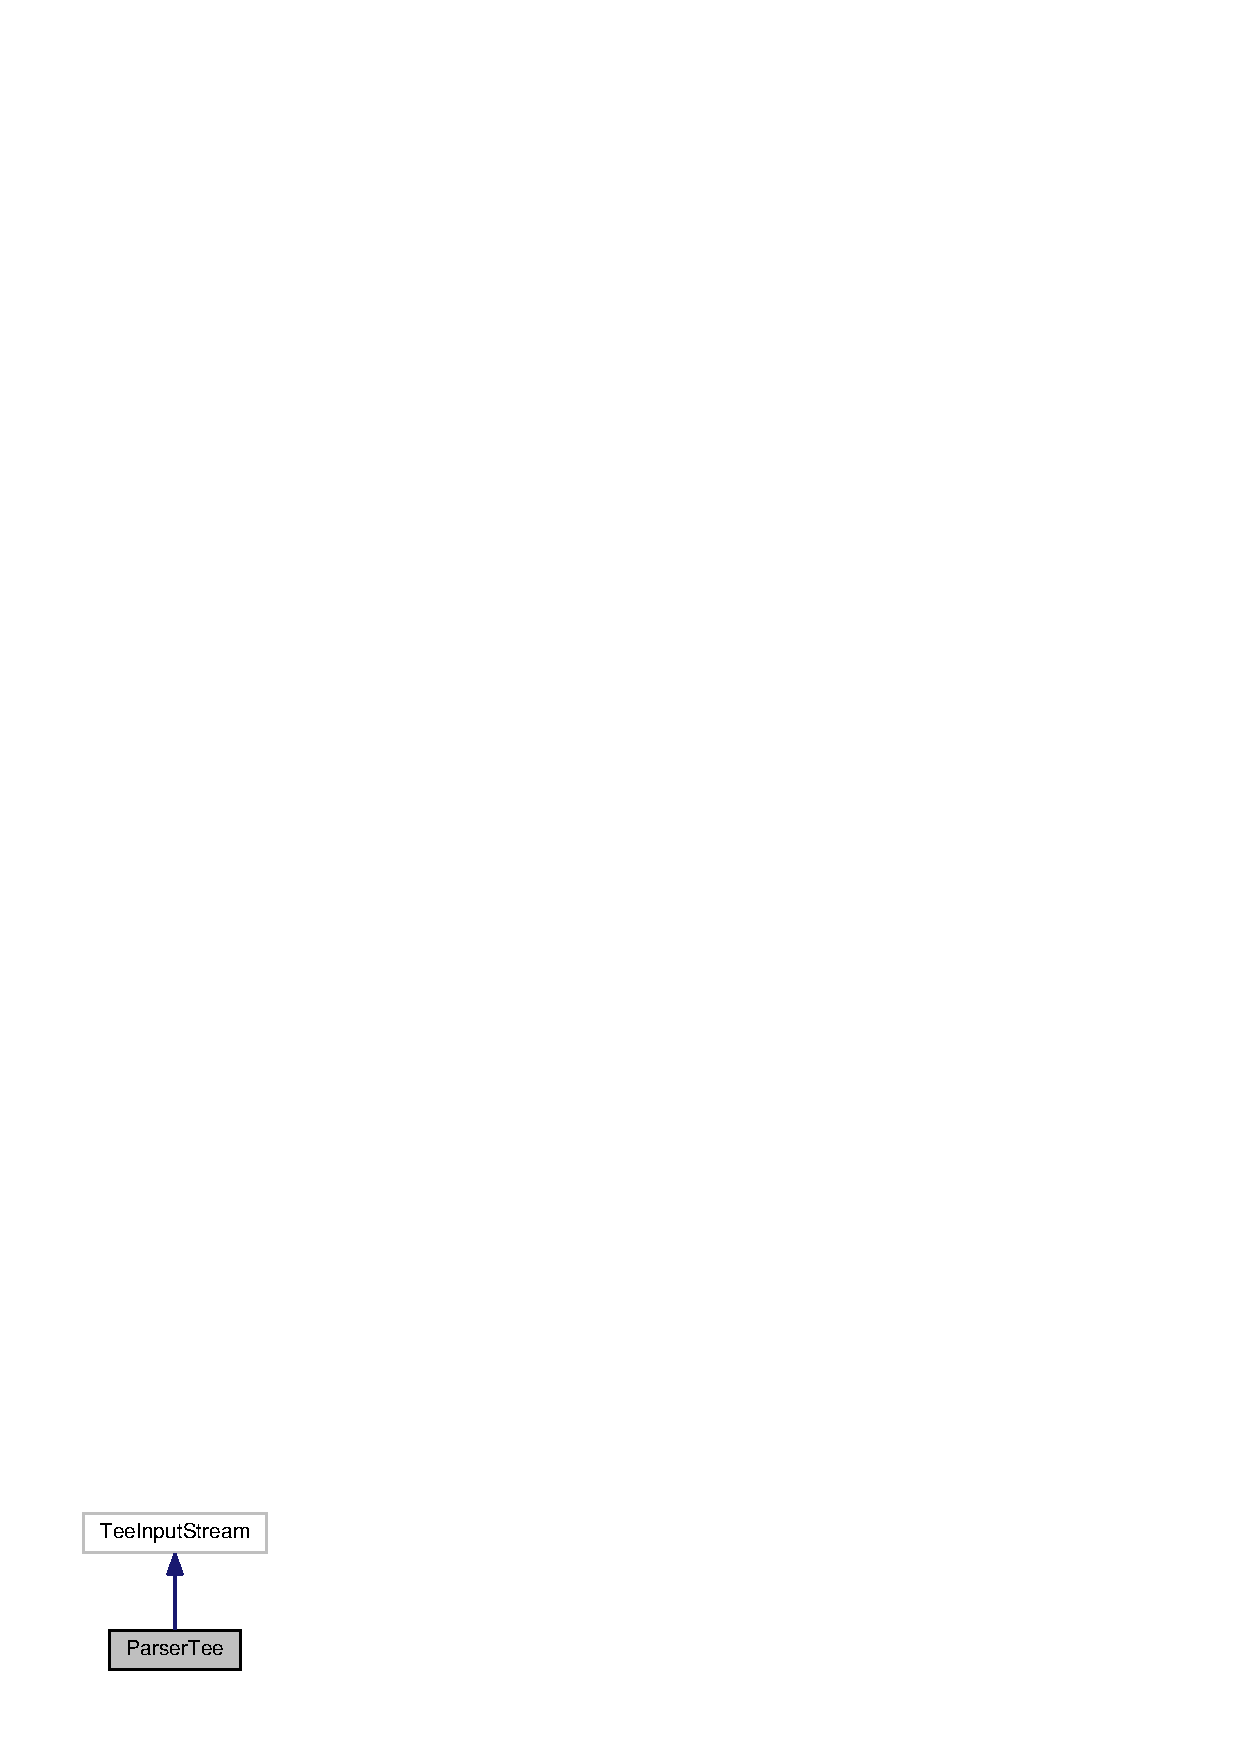
\includegraphics[width=130pt]{classorg_1_1smallfoot_1_1parser_1_1ParserTee__inherit__graph}
\end{center}
\end{figure}


Collaboration diagram for Parser\+Tee\+:\nopagebreak
\begin{figure}[H]
\begin{center}
\leavevmode
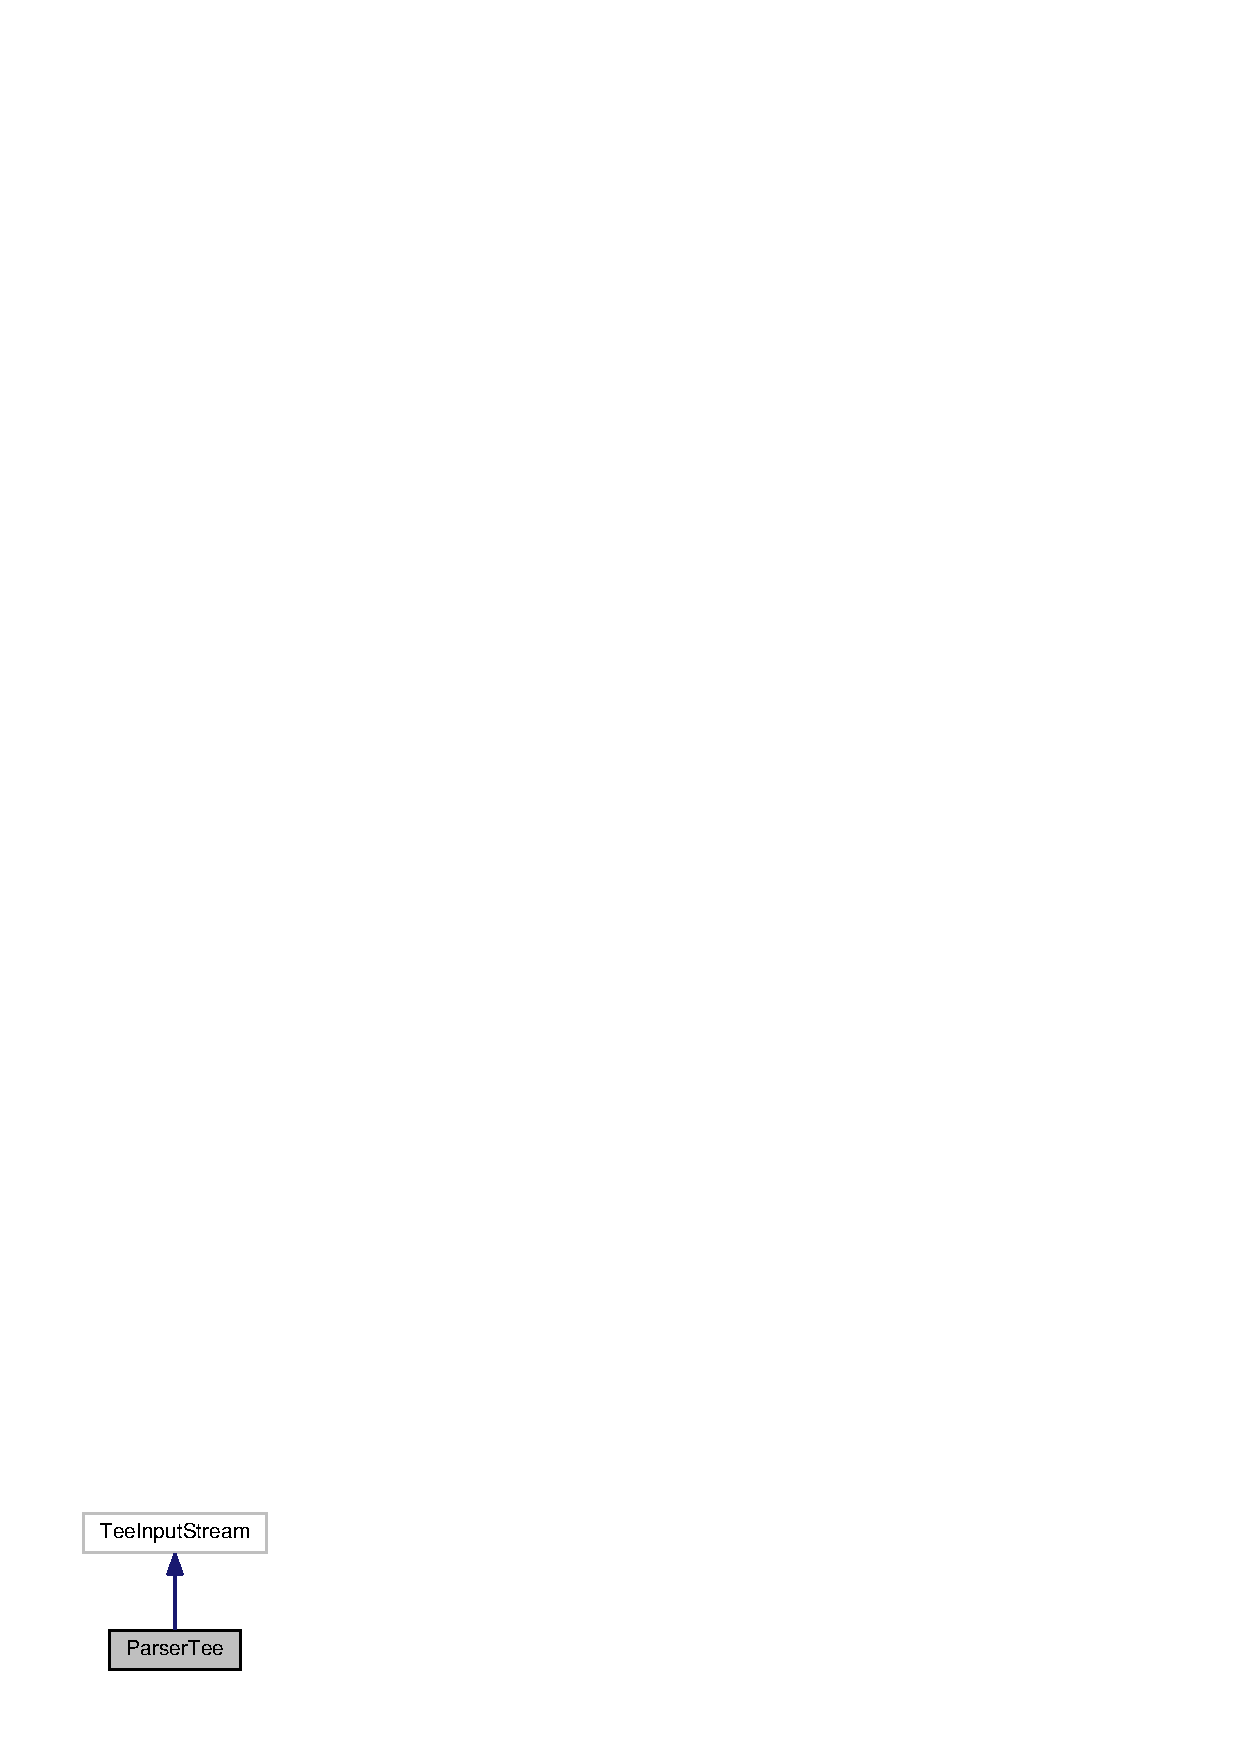
\includegraphics[width=130pt]{classorg_1_1smallfoot_1_1parser_1_1ParserTee__coll__graph}
\end{center}
\end{figure}
\subsection*{Public Member Functions}
\begin{DoxyCompactItemize}
\item 
{\bf Parser\+Tee} (Input\+Stream input, {\bf Zone\+Parser} zp)  throws java.\+io.\+I\+O\+Exception     
\begin{DoxyCompactList}\small\item\em Create a link in a chain of parser tees. \end{DoxyCompactList}\end{DoxyCompactItemize}
\subsection*{Static Public Member Functions}
\begin{DoxyCompactItemize}
\item 
static Output\+Stream {\bf pipe\+Output\+Stream\+To} ({\bf Zone\+Parser} zp)  throws java.\+io.\+I\+O\+Exception     
\begin{DoxyCompactList}\small\item\em Tee off the datastream and set it to sink into the given Zone\+Parser. \end{DoxyCompactList}\end{DoxyCompactItemize}


\subsection{Detailed Description}


Definition at line 11 of file Parser\+Tee.\+java.



\subsection{Constructor \& Destructor Documentation}
\index{org\+::smallfoot\+::parser\+::\+Parser\+Tee@{org\+::smallfoot\+::parser\+::\+Parser\+Tee}!Parser\+Tee@{Parser\+Tee}}
\index{Parser\+Tee@{Parser\+Tee}!org\+::smallfoot\+::parser\+::\+Parser\+Tee@{org\+::smallfoot\+::parser\+::\+Parser\+Tee}}
\subsubsection[{Parser\+Tee}]{\setlength{\rightskip}{0pt plus 5cm}{\bf Parser\+Tee} (
\begin{DoxyParamCaption}
\item[{Input\+Stream}]{input, }
\item[{{\bf Zone\+Parser}}]{zp}
\end{DoxyParamCaption}
) throws java.\+io.\+I\+O\+Exception\hspace{0.3cm}{\ttfamily [inline]}}\label{classorg_1_1smallfoot_1_1parser_1_1ParserTee_a0827a34f92131d39860a9f9df6a4b8c3}


Create a link in a chain of parser tees. 


\begin{DoxyParams}{Parameters}
{\em input} & the incoming datastream to read from and pass through \\
\hline
{\em zp} & a Zone\+Parser to consume a copy of the incoming datastream \\
\hline
\end{DoxyParams}

\begin{DoxyExceptions}{Exceptions}
{\em java.\+io.\+I\+O\+Exception} & if Piped\+Output\+Stream(\+Piped\+Input\+Stream) throws the same \\
\hline
\end{DoxyExceptions}


Definition at line 58 of file Parser\+Tee.\+java.



References Parser\+Tee.\+pipe\+Output\+Stream\+To().



Here is the call graph for this function\+:\nopagebreak
\begin{figure}[H]
\begin{center}
\leavevmode
\includegraphics[width=250pt]{classorg_1_1smallfoot_1_1parser_1_1ParserTee_a0827a34f92131d39860a9f9df6a4b8c3_cgraph}
\end{center}
\end{figure}




\subsection{Member Function Documentation}
\index{org\+::smallfoot\+::parser\+::\+Parser\+Tee@{org\+::smallfoot\+::parser\+::\+Parser\+Tee}!pipe\+Output\+Stream\+To@{pipe\+Output\+Stream\+To}}
\index{pipe\+Output\+Stream\+To@{pipe\+Output\+Stream\+To}!org\+::smallfoot\+::parser\+::\+Parser\+Tee@{org\+::smallfoot\+::parser\+::\+Parser\+Tee}}
\subsubsection[{pipe\+Output\+Stream\+To}]{\setlength{\rightskip}{0pt plus 5cm}static Output\+Stream pipe\+Output\+Stream\+To (
\begin{DoxyParamCaption}
\item[{{\bf Zone\+Parser}}]{zp}
\end{DoxyParamCaption}
) throws java.\+io.\+I\+O\+Exception\hspace{0.3cm}{\ttfamily [inline]}, {\ttfamily [static]}}\label{classorg_1_1smallfoot_1_1parser_1_1ParserTee_a262d09da300622ed145bdd69bbd1a884}


Tee off the datastream and set it to sink into the given Zone\+Parser. 

\begin{DoxyReturn}{Returns}
new Output\+Stream connected to the Zone\+Parser's input to which the tee or fork of the incoming datastream can/should be dumped 
\end{DoxyReturn}

\begin{DoxyParams}{Parameters}
{\em zp} & a Zone\+Parser to consume a copy of the incoming datastream \\
\hline
\end{DoxyParams}

\begin{DoxyExceptions}{Exceptions}
{\em java.\+io.\+I\+O\+Exception} & if Piped\+Output\+Stream(\+Piped\+Input\+Stream) throws the same \\
\hline
\end{DoxyExceptions}


Definition at line 42 of file Parser\+Tee.\+java.



Referenced by Select2\+Sample.\+main(), and Parser\+Tee.\+Parser\+Tee().



The documentation for this class was generated from the following file\+:\begin{DoxyCompactItemize}
\item 
java/{\bf Parser\+Tee.\+java}\end{DoxyCompactItemize}

\section{O\+S\+M\+U\+R\+L\+Connection.\+Result\+C\+S\+V\+Pipe Class Reference}
\label{classorg_1_1smallfoot_1_1parser_1_1osmsql_1_1OSMURLConnection_1_1ResultCSVPipe}\index{O\+S\+M\+U\+R\+L\+Connection.\+Result\+C\+S\+V\+Pipe@{O\+S\+M\+U\+R\+L\+Connection.\+Result\+C\+S\+V\+Pipe}}


Piped\+Output\+Stream to push out resultsets as C\+S\+V Nicknames.  




Inheritance diagram for O\+S\+M\+U\+R\+L\+Connection.\+Result\+C\+S\+V\+Pipe\+:\nopagebreak
\begin{figure}[H]
\begin{center}
\leavevmode
\includegraphics[width=234pt]{classorg_1_1smallfoot_1_1parser_1_1osmsql_1_1OSMURLConnection_1_1ResultCSVPipe__inherit__graph}
\end{center}
\end{figure}


Collaboration diagram for O\+S\+M\+U\+R\+L\+Connection.\+Result\+C\+S\+V\+Pipe\+:\nopagebreak
\begin{figure}[H]
\begin{center}
\leavevmode
\includegraphics[width=234pt]{classorg_1_1smallfoot_1_1parser_1_1osmsql_1_1OSMURLConnection_1_1ResultCSVPipe__coll__graph}
\end{center}
\end{figure}
\subsection*{Public Member Functions}
\begin{DoxyCompactItemize}
\item 
{\bf Result\+C\+S\+V\+Pipe} (java.\+sql.\+Result\+Set {\bf source})
\item 
void {\bf run} ()
\end{DoxyCompactItemize}
\subsection*{Protected Attributes}
\begin{DoxyCompactItemize}
\item 
java.\+sql.\+Result\+Set {\bf source}
\end{DoxyCompactItemize}


\subsection{Detailed Description}
Piped\+Output\+Stream to push out resultsets as C\+S\+V Nicknames. 

No, I\textquotesingle{}m not a fan of this method of doing so, I\textquotesingle{}d rather have the upstream consume data block of W\+W\+N/\+Nickname pairs, but this fits into the stream-\/reading I\textquotesingle{}ve currently got. To be shallow, it fits the current dataflow, although very soon I\textquotesingle{}m sure there will be a need to strip off the layers of hand-\/offs and go with data blocks streaming from various resources. 

Definition at line 42 of file O\+S\+M\+U\+R\+L\+Connection.\+java.



\subsection{Constructor \& Destructor Documentation}
\index{org\+::smallfoot\+::parser\+::osmsql\+::\+O\+S\+M\+U\+R\+L\+Connection\+::\+Result\+C\+S\+V\+Pipe@{org\+::smallfoot\+::parser\+::osmsql\+::\+O\+S\+M\+U\+R\+L\+Connection\+::\+Result\+C\+S\+V\+Pipe}!Result\+C\+S\+V\+Pipe@{Result\+C\+S\+V\+Pipe}}
\index{Result\+C\+S\+V\+Pipe@{Result\+C\+S\+V\+Pipe}!org\+::smallfoot\+::parser\+::osmsql\+::\+O\+S\+M\+U\+R\+L\+Connection\+::\+Result\+C\+S\+V\+Pipe@{org\+::smallfoot\+::parser\+::osmsql\+::\+O\+S\+M\+U\+R\+L\+Connection\+::\+Result\+C\+S\+V\+Pipe}}
\subsubsection[{Result\+C\+S\+V\+Pipe}]{\setlength{\rightskip}{0pt plus 5cm}{\bf Result\+C\+S\+V\+Pipe} (
\begin{DoxyParamCaption}
\item[{java.\+sql.\+Result\+Set}]{source}
\end{DoxyParamCaption}
)\hspace{0.3cm}{\ttfamily [inline]}}\label{classorg_1_1smallfoot_1_1parser_1_1osmsql_1_1OSMURLConnection_1_1ResultCSVPipe_a2d26f904856f6afcdb434ea6d6013288}


Definition at line 46 of file O\+S\+M\+U\+R\+L\+Connection.\+java.



References O\+S\+M\+U\+R\+L\+Connection.\+Result\+C\+S\+V\+Pipe.\+source.



\subsection{Member Function Documentation}
\index{org\+::smallfoot\+::parser\+::osmsql\+::\+O\+S\+M\+U\+R\+L\+Connection\+::\+Result\+C\+S\+V\+Pipe@{org\+::smallfoot\+::parser\+::osmsql\+::\+O\+S\+M\+U\+R\+L\+Connection\+::\+Result\+C\+S\+V\+Pipe}!run@{run}}
\index{run@{run}!org\+::smallfoot\+::parser\+::osmsql\+::\+O\+S\+M\+U\+R\+L\+Connection\+::\+Result\+C\+S\+V\+Pipe@{org\+::smallfoot\+::parser\+::osmsql\+::\+O\+S\+M\+U\+R\+L\+Connection\+::\+Result\+C\+S\+V\+Pipe}}
\subsubsection[{run}]{\setlength{\rightskip}{0pt plus 5cm}void run (
\begin{DoxyParamCaption}
{}
\end{DoxyParamCaption}
)\hspace{0.3cm}{\ttfamily [inline]}}\label{classorg_1_1smallfoot_1_1parser_1_1osmsql_1_1OSMURLConnection_1_1ResultCSVPipe_a13a43e6d814de94978c515cb084873b1}


Definition at line 51 of file O\+S\+M\+U\+R\+L\+Connection.\+java.



References O\+S\+M\+U\+R\+L\+Connection.\+Result\+C\+S\+V\+Pipe.\+source.



\subsection{Field Documentation}
\index{org\+::smallfoot\+::parser\+::osmsql\+::\+O\+S\+M\+U\+R\+L\+Connection\+::\+Result\+C\+S\+V\+Pipe@{org\+::smallfoot\+::parser\+::osmsql\+::\+O\+S\+M\+U\+R\+L\+Connection\+::\+Result\+C\+S\+V\+Pipe}!source@{source}}
\index{source@{source}!org\+::smallfoot\+::parser\+::osmsql\+::\+O\+S\+M\+U\+R\+L\+Connection\+::\+Result\+C\+S\+V\+Pipe@{org\+::smallfoot\+::parser\+::osmsql\+::\+O\+S\+M\+U\+R\+L\+Connection\+::\+Result\+C\+S\+V\+Pipe}}
\subsubsection[{source}]{\setlength{\rightskip}{0pt plus 5cm}java.\+sql.\+Result\+Set source\hspace{0.3cm}{\ttfamily [protected]}}\label{classorg_1_1smallfoot_1_1parser_1_1osmsql_1_1OSMURLConnection_1_1ResultCSVPipe_a0c3a7ce1bb1c3c7b06743537a6b185cf}


Definition at line 44 of file O\+S\+M\+U\+R\+L\+Connection.\+java.



Referenced by O\+S\+M\+U\+R\+L\+Connection.\+Result\+C\+S\+V\+Pipe.\+Result\+C\+S\+V\+Pipe(), and O\+S\+M\+U\+R\+L\+Connection.\+Result\+C\+S\+V\+Pipe.\+run().



The documentation for this class was generated from the following file\+:\begin{DoxyCompactItemize}
\item 
java/{\bf O\+S\+M\+U\+R\+L\+Connection.\+java}\end{DoxyCompactItemize}

\section{Select2\-Sample Class Reference}
\label{classorg_1_1smallfoot_1_1parser_1_1boneheadbits_1_1Select2Sample}\index{Select2\-Sample@{Select2\-Sample}}
\subsection*{Static Public Member Functions}
\begin{DoxyCompactItemize}
\item 
static void {\bf main} (String arg[$\,$])
\end{DoxyCompactItemize}


\subsection{Detailed Description}


Definition at line 10 of file Select2\-Sample.\-java.



\subsection{Member Function Documentation}
\index{org\-::smallfoot\-::parser\-::boneheadbits\-::\-Select2\-Sample@{org\-::smallfoot\-::parser\-::boneheadbits\-::\-Select2\-Sample}!main@{main}}
\index{main@{main}!org::smallfoot::parser::boneheadbits::Select2Sample@{org\-::smallfoot\-::parser\-::boneheadbits\-::\-Select2\-Sample}}
\subsubsection[{main}]{\setlength{\rightskip}{0pt plus 5cm}static void main (
\begin{DoxyParamCaption}
\item[{String}]{arg[$\,$]}
\end{DoxyParamCaption}
)\hspace{0.3cm}{\ttfamily [inline]}, {\ttfamily [static]}}\label{classorg_1_1smallfoot_1_1parser_1_1boneheadbits_1_1Select2Sample_ae4faf7ff4190d227357ef851490d7757}


Definition at line 12 of file Select2\-Sample.\-java.



The documentation for this class was generated from the following file\-:\begin{DoxyCompactItemize}
\item 
java/{\bf Select2\-Sample.\-java}\end{DoxyCompactItemize}

\section{Show\-Zone\-Parser Class Reference}
\label{classorg_1_1smallfoot_1_1parser_1_1zone_1_1ShowZoneParser}\index{Show\-Zone\-Parser@{Show\-Zone\-Parser}}


Inheritance diagram for Show\-Zone\-Parser\-:\nopagebreak
\begin{figure}[H]
\begin{center}
\leavevmode
\includegraphics[width=136pt]{classorg_1_1smallfoot_1_1parser_1_1zone_1_1ShowZoneParser__inherit__graph}
\end{center}
\end{figure}


Collaboration diagram for Show\-Zone\-Parser\-:\nopagebreak
\begin{figure}[H]
\begin{center}
\leavevmode
\includegraphics[width=350pt]{classorg_1_1smallfoot_1_1parser_1_1zone_1_1ShowZoneParser__coll__graph}
\end{center}
\end{figure}
\subsection*{Public Member Functions}
\begin{DoxyCompactItemize}
\item 
void {\bf parse} ()
\item 
void {\bf set\-Reader} (Reader in)
\item 
void {\bf run} ()
\item 
void {\bf set\-Debug} (boolean debug)
\item 
{\bf Show\-Zone\-Parser} (Input\-Stream in, boolean debug\-Me)
\item 
{\bf Show\-Zone\-Parser} (java.\-util.\-Properties in, boolean debug\-Me)
\end{DoxyCompactItemize}
\subsection*{Static Public Member Functions}
\begin{DoxyCompactItemize}
\item 
static void {\bf main} (String args[$\,$])
\end{DoxyCompactItemize}
\subsection*{Static Public Attributes}
\begin{DoxyCompactItemize}
\item 
static final short {\bf A\-L\-P\-H\-A\-N\-U\-M} =257
\item 
static final short {\bf D\-E\-V\-I\-C\-E\-A\-L\-I\-A\-S} =258
\item 
static final short {\bf F\-C\-A\-L\-I\-A\-S} =259
\item 
static final short {\bf N\-A\-M\-E} =260
\item 
static final short {\bf P\-W\-W\-N} =261
\item 
static final short {\bf V\-S\-A\-N} =262
\item 
static final short {\bf Z\-O\-N\-E} =263
\item 
static final short {\bf Y\-Y\-E\-R\-R\-C\-O\-D\-E} =256
\end{DoxyCompactItemize}


\subsection{Detailed Description}


Definition at line 29 of file Show\-Zone\-Parser.\-java.



\subsection{Constructor \& Destructor Documentation}
\index{org\-::smallfoot\-::parser\-::zone\-::\-Show\-Zone\-Parser@{org\-::smallfoot\-::parser\-::zone\-::\-Show\-Zone\-Parser}!Show\-Zone\-Parser@{Show\-Zone\-Parser}}
\index{Show\-Zone\-Parser@{Show\-Zone\-Parser}!org::smallfoot::parser::zone::ShowZoneParser@{org\-::smallfoot\-::parser\-::zone\-::\-Show\-Zone\-Parser}}
\subsubsection[{Show\-Zone\-Parser}]{\setlength{\rightskip}{0pt plus 5cm}{\bf Show\-Zone\-Parser} (
\begin{DoxyParamCaption}
\item[{Input\-Stream}]{in, }
\item[{boolean}]{debug\-Me}
\end{DoxyParamCaption}
)\hspace{0.3cm}{\ttfamily [inline]}}\label{classorg_1_1smallfoot_1_1parser_1_1zone_1_1ShowZoneParser_ad59f06b7fec9a2ac88e1660c2d45289d}


Definition at line 446 of file Show\-Zone\-Parser.\-java.



Referenced by Show\-Zone\-Parser.\-main().

\index{org\-::smallfoot\-::parser\-::zone\-::\-Show\-Zone\-Parser@{org\-::smallfoot\-::parser\-::zone\-::\-Show\-Zone\-Parser}!Show\-Zone\-Parser@{Show\-Zone\-Parser}}
\index{Show\-Zone\-Parser@{Show\-Zone\-Parser}!org::smallfoot::parser::zone::ShowZoneParser@{org\-::smallfoot\-::parser\-::zone\-::\-Show\-Zone\-Parser}}
\subsubsection[{Show\-Zone\-Parser}]{\setlength{\rightskip}{0pt plus 5cm}{\bf Show\-Zone\-Parser} (
\begin{DoxyParamCaption}
\item[{java.\-util.\-Properties}]{in, }
\item[{boolean}]{debug\-Me}
\end{DoxyParamCaption}
)\hspace{0.3cm}{\ttfamily [inline]}}\label{classorg_1_1smallfoot_1_1parser_1_1zone_1_1ShowZoneParser_a08e30aa718b92a9ec99b50be142ab9bc}


Definition at line 447 of file Show\-Zone\-Parser.\-java.



\subsection{Member Function Documentation}
\index{org\-::smallfoot\-::parser\-::zone\-::\-Show\-Zone\-Parser@{org\-::smallfoot\-::parser\-::zone\-::\-Show\-Zone\-Parser}!main@{main}}
\index{main@{main}!org::smallfoot::parser::zone::ShowZoneParser@{org\-::smallfoot\-::parser\-::zone\-::\-Show\-Zone\-Parser}}
\subsubsection[{main}]{\setlength{\rightskip}{0pt plus 5cm}static void main (
\begin{DoxyParamCaption}
\item[{String}]{args[$\,$]}
\end{DoxyParamCaption}
)\hspace{0.3cm}{\ttfamily [inline]}, {\ttfamily [static]}}\label{classorg_1_1smallfoot_1_1parser_1_1zone_1_1ShowZoneParser_a75988cf84fc6ee7a2ebff36e363021aa}


Definition at line 450 of file Show\-Zone\-Parser.\-java.



References Show\-Zone\-Parser.\-Show\-Zone\-Parser().



Here is the call graph for this function\-:\nopagebreak
\begin{figure}[H]
\begin{center}
\leavevmode
\includegraphics[width=212pt]{classorg_1_1smallfoot_1_1parser_1_1zone_1_1ShowZoneParser_a75988cf84fc6ee7a2ebff36e363021aa_cgraph}
\end{center}
\end{figure}


\index{org\-::smallfoot\-::parser\-::zone\-::\-Show\-Zone\-Parser@{org\-::smallfoot\-::parser\-::zone\-::\-Show\-Zone\-Parser}!parse@{parse}}
\index{parse@{parse}!org::smallfoot::parser::zone::ShowZoneParser@{org\-::smallfoot\-::parser\-::zone\-::\-Show\-Zone\-Parser}}
\subsubsection[{parse}]{\setlength{\rightskip}{0pt plus 5cm}void parse (
\begin{DoxyParamCaption}
{}
\end{DoxyParamCaption}
)\hspace{0.3cm}{\ttfamily [inline]}}\label{classorg_1_1smallfoot_1_1parser_1_1zone_1_1ShowZoneParser_ad7c704b34912678d95c13243cacf9d7f}


Definition at line 388 of file Show\-Zone\-Parser.\-java.

\index{org\-::smallfoot\-::parser\-::zone\-::\-Show\-Zone\-Parser@{org\-::smallfoot\-::parser\-::zone\-::\-Show\-Zone\-Parser}!run@{run}}
\index{run@{run}!org::smallfoot::parser::zone::ShowZoneParser@{org\-::smallfoot\-::parser\-::zone\-::\-Show\-Zone\-Parser}}
\subsubsection[{run}]{\setlength{\rightskip}{0pt plus 5cm}void run (
\begin{DoxyParamCaption}
{}
\end{DoxyParamCaption}
)\hspace{0.3cm}{\ttfamily [inline]}}\label{classorg_1_1smallfoot_1_1parser_1_1zone_1_1ShowZoneParser_a13a43e6d814de94978c515cb084873b1}


Definition at line 433 of file Show\-Zone\-Parser.\-java.

\index{org\-::smallfoot\-::parser\-::zone\-::\-Show\-Zone\-Parser@{org\-::smallfoot\-::parser\-::zone\-::\-Show\-Zone\-Parser}!set\-Debug@{set\-Debug}}
\index{set\-Debug@{set\-Debug}!org::smallfoot::parser::zone::ShowZoneParser@{org\-::smallfoot\-::parser\-::zone\-::\-Show\-Zone\-Parser}}
\subsubsection[{set\-Debug}]{\setlength{\rightskip}{0pt plus 5cm}void set\-Debug (
\begin{DoxyParamCaption}
\item[{boolean}]{debug}
\end{DoxyParamCaption}
)\hspace{0.3cm}{\ttfamily [inline]}}\label{classorg_1_1smallfoot_1_1parser_1_1zone_1_1ShowZoneParser_a6c13d260cf71d0554f789c4641a9f18b}


Definition at line 444 of file Show\-Zone\-Parser.\-java.

\index{org\-::smallfoot\-::parser\-::zone\-::\-Show\-Zone\-Parser@{org\-::smallfoot\-::parser\-::zone\-::\-Show\-Zone\-Parser}!set\-Reader@{set\-Reader}}
\index{set\-Reader@{set\-Reader}!org::smallfoot::parser::zone::ShowZoneParser@{org\-::smallfoot\-::parser\-::zone\-::\-Show\-Zone\-Parser}}
\subsubsection[{set\-Reader}]{\setlength{\rightskip}{0pt plus 5cm}void set\-Reader (
\begin{DoxyParamCaption}
\item[{Reader}]{in}
\end{DoxyParamCaption}
)\hspace{0.3cm}{\ttfamily [inline]}}\label{classorg_1_1smallfoot_1_1parser_1_1zone_1_1ShowZoneParser_a5deab139f9ad4072e1a497c5cccda0ea}


Definition at line 400 of file Show\-Zone\-Parser.\-java.



\subsection{Field Documentation}
\index{org\-::smallfoot\-::parser\-::zone\-::\-Show\-Zone\-Parser@{org\-::smallfoot\-::parser\-::zone\-::\-Show\-Zone\-Parser}!A\-L\-P\-H\-A\-N\-U\-M@{A\-L\-P\-H\-A\-N\-U\-M}}
\index{A\-L\-P\-H\-A\-N\-U\-M@{A\-L\-P\-H\-A\-N\-U\-M}!org::smallfoot::parser::zone::ShowZoneParser@{org\-::smallfoot\-::parser\-::zone\-::\-Show\-Zone\-Parser}}
\subsubsection[{A\-L\-P\-H\-A\-N\-U\-M}]{\setlength{\rightskip}{0pt plus 5cm}final short A\-L\-P\-H\-A\-N\-U\-M =257\hspace{0.3cm}{\ttfamily [static]}}\label{classorg_1_1smallfoot_1_1parser_1_1zone_1_1ShowZoneParser_afa1bd945463851953be939c8793faf70}


Definition at line 154 of file Show\-Zone\-Parser.\-java.

\index{org\-::smallfoot\-::parser\-::zone\-::\-Show\-Zone\-Parser@{org\-::smallfoot\-::parser\-::zone\-::\-Show\-Zone\-Parser}!D\-E\-V\-I\-C\-E\-A\-L\-I\-A\-S@{D\-E\-V\-I\-C\-E\-A\-L\-I\-A\-S}}
\index{D\-E\-V\-I\-C\-E\-A\-L\-I\-A\-S@{D\-E\-V\-I\-C\-E\-A\-L\-I\-A\-S}!org::smallfoot::parser::zone::ShowZoneParser@{org\-::smallfoot\-::parser\-::zone\-::\-Show\-Zone\-Parser}}
\subsubsection[{D\-E\-V\-I\-C\-E\-A\-L\-I\-A\-S}]{\setlength{\rightskip}{0pt plus 5cm}final short D\-E\-V\-I\-C\-E\-A\-L\-I\-A\-S =258\hspace{0.3cm}{\ttfamily [static]}}\label{classorg_1_1smallfoot_1_1parser_1_1zone_1_1ShowZoneParser_acabf8c32cf826e213b6e287fd5c70001}


Definition at line 155 of file Show\-Zone\-Parser.\-java.

\index{org\-::smallfoot\-::parser\-::zone\-::\-Show\-Zone\-Parser@{org\-::smallfoot\-::parser\-::zone\-::\-Show\-Zone\-Parser}!F\-C\-A\-L\-I\-A\-S@{F\-C\-A\-L\-I\-A\-S}}
\index{F\-C\-A\-L\-I\-A\-S@{F\-C\-A\-L\-I\-A\-S}!org::smallfoot::parser::zone::ShowZoneParser@{org\-::smallfoot\-::parser\-::zone\-::\-Show\-Zone\-Parser}}
\subsubsection[{F\-C\-A\-L\-I\-A\-S}]{\setlength{\rightskip}{0pt plus 5cm}final short F\-C\-A\-L\-I\-A\-S =259\hspace{0.3cm}{\ttfamily [static]}}\label{classorg_1_1smallfoot_1_1parser_1_1zone_1_1ShowZoneParser_adaff44241832fc6e7ad65dbeb1065d9a}


Definition at line 156 of file Show\-Zone\-Parser.\-java.

\index{org\-::smallfoot\-::parser\-::zone\-::\-Show\-Zone\-Parser@{org\-::smallfoot\-::parser\-::zone\-::\-Show\-Zone\-Parser}!N\-A\-M\-E@{N\-A\-M\-E}}
\index{N\-A\-M\-E@{N\-A\-M\-E}!org::smallfoot::parser::zone::ShowZoneParser@{org\-::smallfoot\-::parser\-::zone\-::\-Show\-Zone\-Parser}}
\subsubsection[{N\-A\-M\-E}]{\setlength{\rightskip}{0pt plus 5cm}final short N\-A\-M\-E =260\hspace{0.3cm}{\ttfamily [static]}}\label{classorg_1_1smallfoot_1_1parser_1_1zone_1_1ShowZoneParser_a66fe0c51d242ca6db52c31bf73a55f8e}


Definition at line 157 of file Show\-Zone\-Parser.\-java.

\index{org\-::smallfoot\-::parser\-::zone\-::\-Show\-Zone\-Parser@{org\-::smallfoot\-::parser\-::zone\-::\-Show\-Zone\-Parser}!P\-W\-W\-N@{P\-W\-W\-N}}
\index{P\-W\-W\-N@{P\-W\-W\-N}!org::smallfoot::parser::zone::ShowZoneParser@{org\-::smallfoot\-::parser\-::zone\-::\-Show\-Zone\-Parser}}
\subsubsection[{P\-W\-W\-N}]{\setlength{\rightskip}{0pt plus 5cm}final short P\-W\-W\-N =261\hspace{0.3cm}{\ttfamily [static]}}\label{classorg_1_1smallfoot_1_1parser_1_1zone_1_1ShowZoneParser_aaa70cc94f40a0785c0ce9ce3cf2ff61d}


Definition at line 158 of file Show\-Zone\-Parser.\-java.

\index{org\-::smallfoot\-::parser\-::zone\-::\-Show\-Zone\-Parser@{org\-::smallfoot\-::parser\-::zone\-::\-Show\-Zone\-Parser}!V\-S\-A\-N@{V\-S\-A\-N}}
\index{V\-S\-A\-N@{V\-S\-A\-N}!org::smallfoot::parser::zone::ShowZoneParser@{org\-::smallfoot\-::parser\-::zone\-::\-Show\-Zone\-Parser}}
\subsubsection[{V\-S\-A\-N}]{\setlength{\rightskip}{0pt plus 5cm}final short V\-S\-A\-N =262\hspace{0.3cm}{\ttfamily [static]}}\label{classorg_1_1smallfoot_1_1parser_1_1zone_1_1ShowZoneParser_a88c9c4c890956fcca92121d318a1a834}


Definition at line 159 of file Show\-Zone\-Parser.\-java.

\index{org\-::smallfoot\-::parser\-::zone\-::\-Show\-Zone\-Parser@{org\-::smallfoot\-::parser\-::zone\-::\-Show\-Zone\-Parser}!Y\-Y\-E\-R\-R\-C\-O\-D\-E@{Y\-Y\-E\-R\-R\-C\-O\-D\-E}}
\index{Y\-Y\-E\-R\-R\-C\-O\-D\-E@{Y\-Y\-E\-R\-R\-C\-O\-D\-E}!org::smallfoot::parser::zone::ShowZoneParser@{org\-::smallfoot\-::parser\-::zone\-::\-Show\-Zone\-Parser}}
\subsubsection[{Y\-Y\-E\-R\-R\-C\-O\-D\-E}]{\setlength{\rightskip}{0pt plus 5cm}final short Y\-Y\-E\-R\-R\-C\-O\-D\-E =256\hspace{0.3cm}{\ttfamily [static]}}\label{classorg_1_1smallfoot_1_1parser_1_1zone_1_1ShowZoneParser_a1c58472ea6621d2f613831e08d10dba3}


Definition at line 161 of file Show\-Zone\-Parser.\-java.

\index{org\-::smallfoot\-::parser\-::zone\-::\-Show\-Zone\-Parser@{org\-::smallfoot\-::parser\-::zone\-::\-Show\-Zone\-Parser}!Z\-O\-N\-E@{Z\-O\-N\-E}}
\index{Z\-O\-N\-E@{Z\-O\-N\-E}!org::smallfoot::parser::zone::ShowZoneParser@{org\-::smallfoot\-::parser\-::zone\-::\-Show\-Zone\-Parser}}
\subsubsection[{Z\-O\-N\-E}]{\setlength{\rightskip}{0pt plus 5cm}final short Z\-O\-N\-E =263\hspace{0.3cm}{\ttfamily [static]}}\label{classorg_1_1smallfoot_1_1parser_1_1zone_1_1ShowZoneParser_a8ddd6c0fce0f972519976a2c9ca1aadd}


Definition at line 160 of file Show\-Zone\-Parser.\-java.



The documentation for this class was generated from the following file\-:\begin{DoxyCompactItemize}
\item 
java/{\bf Show\-Zone\-Parser.\-java}\end{DoxyCompactItemize}

\section{version Class Reference}
\label{classorg_1_1smallfoot_1_1parser_1_1version}\index{version@{version}}
\subsection*{Static Public Member Functions}
\begin{DoxyCompactItemize}
\item 
static void {\bf main} (String arg[$\,$])
\end{DoxyCompactItemize}


\subsection{Detailed Description}


Definition at line 3 of file version.\+java.



\subsection{Member Function Documentation}
\index{org\+::smallfoot\+::parser\+::version@{org\+::smallfoot\+::parser\+::version}!main@{main}}
\index{main@{main}!org\+::smallfoot\+::parser\+::version@{org\+::smallfoot\+::parser\+::version}}
\subsubsection[{main}]{\setlength{\rightskip}{0pt plus 5cm}static void main (
\begin{DoxyParamCaption}
\item[{String}]{arg[$\,$]}
\end{DoxyParamCaption}
)\hspace{0.3cm}{\ttfamily [inline]}, {\ttfamily [static]}}\label{classorg_1_1smallfoot_1_1parser_1_1version_ae4faf7ff4190d227357ef851490d7757}


Definition at line 5 of file version.\+java.



The documentation for this class was generated from the following file\+:\begin{DoxyCompactItemize}
\item 
java/{\bf version.\+java}\end{DoxyCompactItemize}

\section{V\+W4\+Invalid\+Added\+Parser Class Reference}
\label{classorg_1_1smallfoot_1_1parser_1_1zone_1_1VW4InvalidAddedParser}\index{V\+W4\+Invalid\+Added\+Parser@{V\+W4\+Invalid\+Added\+Parser}}


Inheritance diagram for V\+W4\+Invalid\+Added\+Parser\+:\nopagebreak
\begin{figure}[H]
\begin{center}
\leavevmode
\includegraphics[width=168pt]{classorg_1_1smallfoot_1_1parser_1_1zone_1_1VW4InvalidAddedParser__inherit__graph}
\end{center}
\end{figure}


Collaboration diagram for V\+W4\+Invalid\+Added\+Parser\+:\nopagebreak
\begin{figure}[H]
\begin{center}
\leavevmode
\includegraphics[width=350pt]{classorg_1_1smallfoot_1_1parser_1_1zone_1_1VW4InvalidAddedParser__coll__graph}
\end{center}
\end{figure}
\subsection*{Public Member Functions}
\begin{DoxyCompactItemize}
\item 
void {\bf parse} ()
\item 
java.\+util.\+Vector {\bf items} (String name)
\item 
void {\bf add\+Item} (String name, String item)
\item 
void {\bf set\+Reader} (Reader in)
\item 
void {\bf run} ()
\item 
void {\bf set\+Debug} (boolean debug)
\item 
{\bf V\+W4\+Invalid\+Added\+Parser} (Input\+Stream in, boolean debug\+Me)
\item 
{\bf V\+W4\+Invalid\+Added\+Parser} (Input\+Stream in)
\item 
{\bf V\+W4\+Invalid\+Added\+Parser} (java.\+util.\+Properties in)
\end{DoxyCompactItemize}
\subsection*{Static Public Member Functions}
\begin{DoxyCompactItemize}
\item 
static void {\bf main} (String args[$\,$])
\end{DoxyCompactItemize}
\subsection*{Static Public Attributes}
\begin{DoxyCompactItemize}
\item 
static final short {\bf A\+L\+P\+H\+A\+N\+U\+M} =257
\item 
static final short {\bf A\+L\+R\+E\+A\+D\+Y} =258
\item 
static final short {\bf A\+D\+D\+E\+D} =259
\item 
static final short {\bf C\+H\+I\+L\+D} =260
\item 
static final short {\bf C\+O\+L\+U\+M\+N} =261
\item 
static final short {\bf D\+I\+S\+C\+O\+V\+E\+R\+E\+D} =262
\item 
static final short {\bf D\+U\+P\+L\+I\+C\+A\+T\+E} =263
\item 
static final short {\bf E\+D\+I\+T} =264
\item 
static final short {\bf E\+X\+I\+S\+T} =265
\item 
static final short {\bf E\+N\+T\+I\+T\+I\+E\+S} =266
\item 
static final short {\bf E\+N\+T\+I\+T\+Y} =267
\item 
static final short {\bf F\+C\+P\+O\+R\+T} =268
\item 
static final short {\bf G\+I\+V\+E\+N} =269
\item 
static final short {\bf H\+B\+A} =270
\item 
static final short {\bf H\+O\+S\+T} =271
\item 
static final short {\bf I\+N\+V\+A\+L\+I\+D} =272
\item 
static final short {\bf I\+O\+M\+O\+D\+U\+L\+E} =273
\item 
static final short {\bf L\+I\+N\+E} =274
\item 
static final short {\bf L\+O\+C\+A\+T\+I\+O\+N} =275
\item 
static final short {\bf M\+O\+D\+I\+F\+Y} =276
\item 
static final short {\bf N\+A\+M\+E} =277
\item 
static final short {\bf N\+E\+W} =278
\item 
static final short {\bf O\+V\+E\+R\+W\+R\+I\+T\+E} =279
\item 
static final short {\bf P\+O\+R\+T} =280
\item 
static final short {\bf S\+T\+O\+R\+A\+G\+E\+A\+R\+R\+A\+Y} =281
\item 
static final short {\bf S\+T\+O\+R\+A\+G\+E\+C\+O\+N\+T\+R\+O\+L\+L\+E\+R} =282
\item 
static final short {\bf T\+O} =283
\item 
static final short {\bf T\+Y\+P\+E} =284
\item 
static final short {\bf U\+S\+E} =285
\item 
static final short {\bf W\+I\+T\+H} =286
\item 
static final short {\bf W\+W\+P\+N} =287
\item 
static final short {\bf Y\+Y\+E\+R\+R\+C\+O\+D\+E} =256
\end{DoxyCompactItemize}


\subsection{Detailed Description}


Definition at line 63 of file V\+W4\+Invalid\+Added\+Parser.\+java.



\subsection{Constructor \& Destructor Documentation}
\index{org\+::smallfoot\+::parser\+::zone\+::\+V\+W4\+Invalid\+Added\+Parser@{org\+::smallfoot\+::parser\+::zone\+::\+V\+W4\+Invalid\+Added\+Parser}!V\+W4\+Invalid\+Added\+Parser@{V\+W4\+Invalid\+Added\+Parser}}
\index{V\+W4\+Invalid\+Added\+Parser@{V\+W4\+Invalid\+Added\+Parser}!org\+::smallfoot\+::parser\+::zone\+::\+V\+W4\+Invalid\+Added\+Parser@{org\+::smallfoot\+::parser\+::zone\+::\+V\+W4\+Invalid\+Added\+Parser}}
\subsubsection[{V\+W4\+Invalid\+Added\+Parser}]{\setlength{\rightskip}{0pt plus 5cm}{\bf V\+W4\+Invalid\+Added\+Parser} (
\begin{DoxyParamCaption}
\item[{Input\+Stream}]{in, }
\item[{boolean}]{debug\+Me}
\end{DoxyParamCaption}
)\hspace{0.3cm}{\ttfamily [inline]}}\label{classorg_1_1smallfoot_1_1parser_1_1zone_1_1VW4InvalidAddedParser_a883f64011f4bd6ffb448ae0eaac1bcda}


Definition at line 756 of file V\+W4\+Invalid\+Added\+Parser.\+java.



Referenced by V\+W4\+Invalid\+Added\+Parser.\+main().

\index{org\+::smallfoot\+::parser\+::zone\+::\+V\+W4\+Invalid\+Added\+Parser@{org\+::smallfoot\+::parser\+::zone\+::\+V\+W4\+Invalid\+Added\+Parser}!V\+W4\+Invalid\+Added\+Parser@{V\+W4\+Invalid\+Added\+Parser}}
\index{V\+W4\+Invalid\+Added\+Parser@{V\+W4\+Invalid\+Added\+Parser}!org\+::smallfoot\+::parser\+::zone\+::\+V\+W4\+Invalid\+Added\+Parser@{org\+::smallfoot\+::parser\+::zone\+::\+V\+W4\+Invalid\+Added\+Parser}}
\subsubsection[{V\+W4\+Invalid\+Added\+Parser}]{\setlength{\rightskip}{0pt plus 5cm}{\bf V\+W4\+Invalid\+Added\+Parser} (
\begin{DoxyParamCaption}
\item[{Input\+Stream}]{in}
\end{DoxyParamCaption}
)\hspace{0.3cm}{\ttfamily [inline]}}\label{classorg_1_1smallfoot_1_1parser_1_1zone_1_1VW4InvalidAddedParser_aceee193982e5d541a3a302bdf288cb0a}


Definition at line 760 of file V\+W4\+Invalid\+Added\+Parser.\+java.

\index{org\+::smallfoot\+::parser\+::zone\+::\+V\+W4\+Invalid\+Added\+Parser@{org\+::smallfoot\+::parser\+::zone\+::\+V\+W4\+Invalid\+Added\+Parser}!V\+W4\+Invalid\+Added\+Parser@{V\+W4\+Invalid\+Added\+Parser}}
\index{V\+W4\+Invalid\+Added\+Parser@{V\+W4\+Invalid\+Added\+Parser}!org\+::smallfoot\+::parser\+::zone\+::\+V\+W4\+Invalid\+Added\+Parser@{org\+::smallfoot\+::parser\+::zone\+::\+V\+W4\+Invalid\+Added\+Parser}}
\subsubsection[{V\+W4\+Invalid\+Added\+Parser}]{\setlength{\rightskip}{0pt plus 5cm}{\bf V\+W4\+Invalid\+Added\+Parser} (
\begin{DoxyParamCaption}
\item[{java.\+util.\+Properties}]{in}
\end{DoxyParamCaption}
)\hspace{0.3cm}{\ttfamily [inline]}}\label{classorg_1_1smallfoot_1_1parser_1_1zone_1_1VW4InvalidAddedParser_a137efd4997364aa3550fbbd28fe8354a}


Definition at line 764 of file V\+W4\+Invalid\+Added\+Parser.\+java.



\subsection{Member Function Documentation}
\index{org\+::smallfoot\+::parser\+::zone\+::\+V\+W4\+Invalid\+Added\+Parser@{org\+::smallfoot\+::parser\+::zone\+::\+V\+W4\+Invalid\+Added\+Parser}!add\+Item@{add\+Item}}
\index{add\+Item@{add\+Item}!org\+::smallfoot\+::parser\+::zone\+::\+V\+W4\+Invalid\+Added\+Parser@{org\+::smallfoot\+::parser\+::zone\+::\+V\+W4\+Invalid\+Added\+Parser}}
\subsubsection[{add\+Item}]{\setlength{\rightskip}{0pt plus 5cm}void add\+Item (
\begin{DoxyParamCaption}
\item[{String}]{name, }
\item[{String}]{item}
\end{DoxyParamCaption}
)\hspace{0.3cm}{\ttfamily [inline]}}\label{classorg_1_1smallfoot_1_1parser_1_1zone_1_1VW4InvalidAddedParser_a66ee8ab84d5c5705c2ddf0c60cb3c2a3}


Definition at line 693 of file V\+W4\+Invalid\+Added\+Parser.\+java.

\index{org\+::smallfoot\+::parser\+::zone\+::\+V\+W4\+Invalid\+Added\+Parser@{org\+::smallfoot\+::parser\+::zone\+::\+V\+W4\+Invalid\+Added\+Parser}!items@{items}}
\index{items@{items}!org\+::smallfoot\+::parser\+::zone\+::\+V\+W4\+Invalid\+Added\+Parser@{org\+::smallfoot\+::parser\+::zone\+::\+V\+W4\+Invalid\+Added\+Parser}}
\subsubsection[{items}]{\setlength{\rightskip}{0pt plus 5cm}java.\+util.\+Vector items (
\begin{DoxyParamCaption}
\item[{String}]{name}
\end{DoxyParamCaption}
)\hspace{0.3cm}{\ttfamily [inline]}}\label{classorg_1_1smallfoot_1_1parser_1_1zone_1_1VW4InvalidAddedParser_af0a81691449a6211ef6b9ffc8b62bb0a}


Definition at line 686 of file V\+W4\+Invalid\+Added\+Parser.\+java.

\index{org\+::smallfoot\+::parser\+::zone\+::\+V\+W4\+Invalid\+Added\+Parser@{org\+::smallfoot\+::parser\+::zone\+::\+V\+W4\+Invalid\+Added\+Parser}!main@{main}}
\index{main@{main}!org\+::smallfoot\+::parser\+::zone\+::\+V\+W4\+Invalid\+Added\+Parser@{org\+::smallfoot\+::parser\+::zone\+::\+V\+W4\+Invalid\+Added\+Parser}}
\subsubsection[{main}]{\setlength{\rightskip}{0pt plus 5cm}static void main (
\begin{DoxyParamCaption}
\item[{String}]{args[$\,$]}
\end{DoxyParamCaption}
)\hspace{0.3cm}{\ttfamily [inline]}, {\ttfamily [static]}}\label{classorg_1_1smallfoot_1_1parser_1_1zone_1_1VW4InvalidAddedParser_a75988cf84fc6ee7a2ebff36e363021aa}


Definition at line 770 of file V\+W4\+Invalid\+Added\+Parser.\+java.



References Zone\+Parser\+I.\+test\+Summary(), and V\+W4\+Invalid\+Added\+Parser.\+V\+W4\+Invalid\+Added\+Parser().



Here is the call graph for this function\+:\nopagebreak
\begin{figure}[H]
\begin{center}
\leavevmode
\includegraphics[width=350pt]{classorg_1_1smallfoot_1_1parser_1_1zone_1_1VW4InvalidAddedParser_a75988cf84fc6ee7a2ebff36e363021aa_cgraph}
\end{center}
\end{figure}


\index{org\+::smallfoot\+::parser\+::zone\+::\+V\+W4\+Invalid\+Added\+Parser@{org\+::smallfoot\+::parser\+::zone\+::\+V\+W4\+Invalid\+Added\+Parser}!parse@{parse}}
\index{parse@{parse}!org\+::smallfoot\+::parser\+::zone\+::\+V\+W4\+Invalid\+Added\+Parser@{org\+::smallfoot\+::parser\+::zone\+::\+V\+W4\+Invalid\+Added\+Parser}}
\subsubsection[{parse}]{\setlength{\rightskip}{0pt plus 5cm}void parse (
\begin{DoxyParamCaption}
{}
\end{DoxyParamCaption}
)\hspace{0.3cm}{\ttfamily [inline]}}\label{classorg_1_1smallfoot_1_1parser_1_1zone_1_1VW4InvalidAddedParser_ad7c704b34912678d95c13243cacf9d7f}


Definition at line 673 of file V\+W4\+Invalid\+Added\+Parser.\+java.

\index{org\+::smallfoot\+::parser\+::zone\+::\+V\+W4\+Invalid\+Added\+Parser@{org\+::smallfoot\+::parser\+::zone\+::\+V\+W4\+Invalid\+Added\+Parser}!run@{run}}
\index{run@{run}!org\+::smallfoot\+::parser\+::zone\+::\+V\+W4\+Invalid\+Added\+Parser@{org\+::smallfoot\+::parser\+::zone\+::\+V\+W4\+Invalid\+Added\+Parser}}
\subsubsection[{run}]{\setlength{\rightskip}{0pt plus 5cm}void run (
\begin{DoxyParamCaption}
{}
\end{DoxyParamCaption}
)\hspace{0.3cm}{\ttfamily [inline]}}\label{classorg_1_1smallfoot_1_1parser_1_1zone_1_1VW4InvalidAddedParser_a13a43e6d814de94978c515cb084873b1}


Definition at line 737 of file V\+W4\+Invalid\+Added\+Parser.\+java.

\index{org\+::smallfoot\+::parser\+::zone\+::\+V\+W4\+Invalid\+Added\+Parser@{org\+::smallfoot\+::parser\+::zone\+::\+V\+W4\+Invalid\+Added\+Parser}!set\+Debug@{set\+Debug}}
\index{set\+Debug@{set\+Debug}!org\+::smallfoot\+::parser\+::zone\+::\+V\+W4\+Invalid\+Added\+Parser@{org\+::smallfoot\+::parser\+::zone\+::\+V\+W4\+Invalid\+Added\+Parser}}
\subsubsection[{set\+Debug}]{\setlength{\rightskip}{0pt plus 5cm}void set\+Debug (
\begin{DoxyParamCaption}
\item[{boolean}]{debug}
\end{DoxyParamCaption}
)\hspace{0.3cm}{\ttfamily [inline]}}\label{classorg_1_1smallfoot_1_1parser_1_1zone_1_1VW4InvalidAddedParser_a6c13d260cf71d0554f789c4641a9f18b}


Definition at line 752 of file V\+W4\+Invalid\+Added\+Parser.\+java.

\index{org\+::smallfoot\+::parser\+::zone\+::\+V\+W4\+Invalid\+Added\+Parser@{org\+::smallfoot\+::parser\+::zone\+::\+V\+W4\+Invalid\+Added\+Parser}!set\+Reader@{set\+Reader}}
\index{set\+Reader@{set\+Reader}!org\+::smallfoot\+::parser\+::zone\+::\+V\+W4\+Invalid\+Added\+Parser@{org\+::smallfoot\+::parser\+::zone\+::\+V\+W4\+Invalid\+Added\+Parser}}
\subsubsection[{set\+Reader}]{\setlength{\rightskip}{0pt plus 5cm}void set\+Reader (
\begin{DoxyParamCaption}
\item[{Reader}]{in}
\end{DoxyParamCaption}
)\hspace{0.3cm}{\ttfamily [inline]}}\label{classorg_1_1smallfoot_1_1parser_1_1zone_1_1VW4InvalidAddedParser_a5deab139f9ad4072e1a497c5cccda0ea}


Definition at line 704 of file V\+W4\+Invalid\+Added\+Parser.\+java.



\subsection{Field Documentation}
\index{org\+::smallfoot\+::parser\+::zone\+::\+V\+W4\+Invalid\+Added\+Parser@{org\+::smallfoot\+::parser\+::zone\+::\+V\+W4\+Invalid\+Added\+Parser}!A\+D\+D\+E\+D@{A\+D\+D\+E\+D}}
\index{A\+D\+D\+E\+D@{A\+D\+D\+E\+D}!org\+::smallfoot\+::parser\+::zone\+::\+V\+W4\+Invalid\+Added\+Parser@{org\+::smallfoot\+::parser\+::zone\+::\+V\+W4\+Invalid\+Added\+Parser}}
\subsubsection[{A\+D\+D\+E\+D}]{\setlength{\rightskip}{0pt plus 5cm}final short A\+D\+D\+E\+D =259\hspace{0.3cm}{\ttfamily [static]}}\label{classorg_1_1smallfoot_1_1parser_1_1zone_1_1VW4InvalidAddedParser_a47f0373b201de53529ea39cfdb320a9a}


Definition at line 194 of file V\+W4\+Invalid\+Added\+Parser.\+java.

\index{org\+::smallfoot\+::parser\+::zone\+::\+V\+W4\+Invalid\+Added\+Parser@{org\+::smallfoot\+::parser\+::zone\+::\+V\+W4\+Invalid\+Added\+Parser}!A\+L\+P\+H\+A\+N\+U\+M@{A\+L\+P\+H\+A\+N\+U\+M}}
\index{A\+L\+P\+H\+A\+N\+U\+M@{A\+L\+P\+H\+A\+N\+U\+M}!org\+::smallfoot\+::parser\+::zone\+::\+V\+W4\+Invalid\+Added\+Parser@{org\+::smallfoot\+::parser\+::zone\+::\+V\+W4\+Invalid\+Added\+Parser}}
\subsubsection[{A\+L\+P\+H\+A\+N\+U\+M}]{\setlength{\rightskip}{0pt plus 5cm}final short A\+L\+P\+H\+A\+N\+U\+M =257\hspace{0.3cm}{\ttfamily [static]}}\label{classorg_1_1smallfoot_1_1parser_1_1zone_1_1VW4InvalidAddedParser_afa1bd945463851953be939c8793faf70}


Definition at line 192 of file V\+W4\+Invalid\+Added\+Parser.\+java.

\index{org\+::smallfoot\+::parser\+::zone\+::\+V\+W4\+Invalid\+Added\+Parser@{org\+::smallfoot\+::parser\+::zone\+::\+V\+W4\+Invalid\+Added\+Parser}!A\+L\+R\+E\+A\+D\+Y@{A\+L\+R\+E\+A\+D\+Y}}
\index{A\+L\+R\+E\+A\+D\+Y@{A\+L\+R\+E\+A\+D\+Y}!org\+::smallfoot\+::parser\+::zone\+::\+V\+W4\+Invalid\+Added\+Parser@{org\+::smallfoot\+::parser\+::zone\+::\+V\+W4\+Invalid\+Added\+Parser}}
\subsubsection[{A\+L\+R\+E\+A\+D\+Y}]{\setlength{\rightskip}{0pt plus 5cm}final short A\+L\+R\+E\+A\+D\+Y =258\hspace{0.3cm}{\ttfamily [static]}}\label{classorg_1_1smallfoot_1_1parser_1_1zone_1_1VW4InvalidAddedParser_a3bf756aa7c437ba6a6a0e7e6424199ec}


Definition at line 193 of file V\+W4\+Invalid\+Added\+Parser.\+java.

\index{org\+::smallfoot\+::parser\+::zone\+::\+V\+W4\+Invalid\+Added\+Parser@{org\+::smallfoot\+::parser\+::zone\+::\+V\+W4\+Invalid\+Added\+Parser}!C\+H\+I\+L\+D@{C\+H\+I\+L\+D}}
\index{C\+H\+I\+L\+D@{C\+H\+I\+L\+D}!org\+::smallfoot\+::parser\+::zone\+::\+V\+W4\+Invalid\+Added\+Parser@{org\+::smallfoot\+::parser\+::zone\+::\+V\+W4\+Invalid\+Added\+Parser}}
\subsubsection[{C\+H\+I\+L\+D}]{\setlength{\rightskip}{0pt plus 5cm}final short C\+H\+I\+L\+D =260\hspace{0.3cm}{\ttfamily [static]}}\label{classorg_1_1smallfoot_1_1parser_1_1zone_1_1VW4InvalidAddedParser_a88f4cd11b8a94e957069b64101ff8f09}


Definition at line 195 of file V\+W4\+Invalid\+Added\+Parser.\+java.

\index{org\+::smallfoot\+::parser\+::zone\+::\+V\+W4\+Invalid\+Added\+Parser@{org\+::smallfoot\+::parser\+::zone\+::\+V\+W4\+Invalid\+Added\+Parser}!C\+O\+L\+U\+M\+N@{C\+O\+L\+U\+M\+N}}
\index{C\+O\+L\+U\+M\+N@{C\+O\+L\+U\+M\+N}!org\+::smallfoot\+::parser\+::zone\+::\+V\+W4\+Invalid\+Added\+Parser@{org\+::smallfoot\+::parser\+::zone\+::\+V\+W4\+Invalid\+Added\+Parser}}
\subsubsection[{C\+O\+L\+U\+M\+N}]{\setlength{\rightskip}{0pt plus 5cm}final short C\+O\+L\+U\+M\+N =261\hspace{0.3cm}{\ttfamily [static]}}\label{classorg_1_1smallfoot_1_1parser_1_1zone_1_1VW4InvalidAddedParser_a393daa759a1143577ed9c520408718e9}


Definition at line 196 of file V\+W4\+Invalid\+Added\+Parser.\+java.

\index{org\+::smallfoot\+::parser\+::zone\+::\+V\+W4\+Invalid\+Added\+Parser@{org\+::smallfoot\+::parser\+::zone\+::\+V\+W4\+Invalid\+Added\+Parser}!D\+I\+S\+C\+O\+V\+E\+R\+E\+D@{D\+I\+S\+C\+O\+V\+E\+R\+E\+D}}
\index{D\+I\+S\+C\+O\+V\+E\+R\+E\+D@{D\+I\+S\+C\+O\+V\+E\+R\+E\+D}!org\+::smallfoot\+::parser\+::zone\+::\+V\+W4\+Invalid\+Added\+Parser@{org\+::smallfoot\+::parser\+::zone\+::\+V\+W4\+Invalid\+Added\+Parser}}
\subsubsection[{D\+I\+S\+C\+O\+V\+E\+R\+E\+D}]{\setlength{\rightskip}{0pt plus 5cm}final short D\+I\+S\+C\+O\+V\+E\+R\+E\+D =262\hspace{0.3cm}{\ttfamily [static]}}\label{classorg_1_1smallfoot_1_1parser_1_1zone_1_1VW4InvalidAddedParser_ab8deb1199b66df49d12f84442cb8de2e}


Definition at line 197 of file V\+W4\+Invalid\+Added\+Parser.\+java.

\index{org\+::smallfoot\+::parser\+::zone\+::\+V\+W4\+Invalid\+Added\+Parser@{org\+::smallfoot\+::parser\+::zone\+::\+V\+W4\+Invalid\+Added\+Parser}!D\+U\+P\+L\+I\+C\+A\+T\+E@{D\+U\+P\+L\+I\+C\+A\+T\+E}}
\index{D\+U\+P\+L\+I\+C\+A\+T\+E@{D\+U\+P\+L\+I\+C\+A\+T\+E}!org\+::smallfoot\+::parser\+::zone\+::\+V\+W4\+Invalid\+Added\+Parser@{org\+::smallfoot\+::parser\+::zone\+::\+V\+W4\+Invalid\+Added\+Parser}}
\subsubsection[{D\+U\+P\+L\+I\+C\+A\+T\+E}]{\setlength{\rightskip}{0pt plus 5cm}final short D\+U\+P\+L\+I\+C\+A\+T\+E =263\hspace{0.3cm}{\ttfamily [static]}}\label{classorg_1_1smallfoot_1_1parser_1_1zone_1_1VW4InvalidAddedParser_a142e251b5aa41d18d88b73c6be2e269d}


Definition at line 198 of file V\+W4\+Invalid\+Added\+Parser.\+java.

\index{org\+::smallfoot\+::parser\+::zone\+::\+V\+W4\+Invalid\+Added\+Parser@{org\+::smallfoot\+::parser\+::zone\+::\+V\+W4\+Invalid\+Added\+Parser}!E\+D\+I\+T@{E\+D\+I\+T}}
\index{E\+D\+I\+T@{E\+D\+I\+T}!org\+::smallfoot\+::parser\+::zone\+::\+V\+W4\+Invalid\+Added\+Parser@{org\+::smallfoot\+::parser\+::zone\+::\+V\+W4\+Invalid\+Added\+Parser}}
\subsubsection[{E\+D\+I\+T}]{\setlength{\rightskip}{0pt plus 5cm}final short E\+D\+I\+T =264\hspace{0.3cm}{\ttfamily [static]}}\label{classorg_1_1smallfoot_1_1parser_1_1zone_1_1VW4InvalidAddedParser_a1902040f07e240e77bb1ba5549f2b745}


Definition at line 199 of file V\+W4\+Invalid\+Added\+Parser.\+java.

\index{org\+::smallfoot\+::parser\+::zone\+::\+V\+W4\+Invalid\+Added\+Parser@{org\+::smallfoot\+::parser\+::zone\+::\+V\+W4\+Invalid\+Added\+Parser}!E\+N\+T\+I\+T\+I\+E\+S@{E\+N\+T\+I\+T\+I\+E\+S}}
\index{E\+N\+T\+I\+T\+I\+E\+S@{E\+N\+T\+I\+T\+I\+E\+S}!org\+::smallfoot\+::parser\+::zone\+::\+V\+W4\+Invalid\+Added\+Parser@{org\+::smallfoot\+::parser\+::zone\+::\+V\+W4\+Invalid\+Added\+Parser}}
\subsubsection[{E\+N\+T\+I\+T\+I\+E\+S}]{\setlength{\rightskip}{0pt plus 5cm}final short E\+N\+T\+I\+T\+I\+E\+S =266\hspace{0.3cm}{\ttfamily [static]}}\label{classorg_1_1smallfoot_1_1parser_1_1zone_1_1VW4InvalidAddedParser_a7d254cfa99265d281a12aca532b81672}


Definition at line 201 of file V\+W4\+Invalid\+Added\+Parser.\+java.

\index{org\+::smallfoot\+::parser\+::zone\+::\+V\+W4\+Invalid\+Added\+Parser@{org\+::smallfoot\+::parser\+::zone\+::\+V\+W4\+Invalid\+Added\+Parser}!E\+N\+T\+I\+T\+Y@{E\+N\+T\+I\+T\+Y}}
\index{E\+N\+T\+I\+T\+Y@{E\+N\+T\+I\+T\+Y}!org\+::smallfoot\+::parser\+::zone\+::\+V\+W4\+Invalid\+Added\+Parser@{org\+::smallfoot\+::parser\+::zone\+::\+V\+W4\+Invalid\+Added\+Parser}}
\subsubsection[{E\+N\+T\+I\+T\+Y}]{\setlength{\rightskip}{0pt plus 5cm}final short E\+N\+T\+I\+T\+Y =267\hspace{0.3cm}{\ttfamily [static]}}\label{classorg_1_1smallfoot_1_1parser_1_1zone_1_1VW4InvalidAddedParser_a24aaff68b061db04aba7d2161699b139}


Definition at line 202 of file V\+W4\+Invalid\+Added\+Parser.\+java.

\index{org\+::smallfoot\+::parser\+::zone\+::\+V\+W4\+Invalid\+Added\+Parser@{org\+::smallfoot\+::parser\+::zone\+::\+V\+W4\+Invalid\+Added\+Parser}!E\+X\+I\+S\+T@{E\+X\+I\+S\+T}}
\index{E\+X\+I\+S\+T@{E\+X\+I\+S\+T}!org\+::smallfoot\+::parser\+::zone\+::\+V\+W4\+Invalid\+Added\+Parser@{org\+::smallfoot\+::parser\+::zone\+::\+V\+W4\+Invalid\+Added\+Parser}}
\subsubsection[{E\+X\+I\+S\+T}]{\setlength{\rightskip}{0pt plus 5cm}final short E\+X\+I\+S\+T =265\hspace{0.3cm}{\ttfamily [static]}}\label{classorg_1_1smallfoot_1_1parser_1_1zone_1_1VW4InvalidAddedParser_a4a662f099a679e179bb1b75d11cd2a12}


Definition at line 200 of file V\+W4\+Invalid\+Added\+Parser.\+java.

\index{org\+::smallfoot\+::parser\+::zone\+::\+V\+W4\+Invalid\+Added\+Parser@{org\+::smallfoot\+::parser\+::zone\+::\+V\+W4\+Invalid\+Added\+Parser}!F\+C\+P\+O\+R\+T@{F\+C\+P\+O\+R\+T}}
\index{F\+C\+P\+O\+R\+T@{F\+C\+P\+O\+R\+T}!org\+::smallfoot\+::parser\+::zone\+::\+V\+W4\+Invalid\+Added\+Parser@{org\+::smallfoot\+::parser\+::zone\+::\+V\+W4\+Invalid\+Added\+Parser}}
\subsubsection[{F\+C\+P\+O\+R\+T}]{\setlength{\rightskip}{0pt plus 5cm}final short F\+C\+P\+O\+R\+T =268\hspace{0.3cm}{\ttfamily [static]}}\label{classorg_1_1smallfoot_1_1parser_1_1zone_1_1VW4InvalidAddedParser_a6930494544f9c86e15f42f3790bac9e6}


Definition at line 203 of file V\+W4\+Invalid\+Added\+Parser.\+java.

\index{org\+::smallfoot\+::parser\+::zone\+::\+V\+W4\+Invalid\+Added\+Parser@{org\+::smallfoot\+::parser\+::zone\+::\+V\+W4\+Invalid\+Added\+Parser}!G\+I\+V\+E\+N@{G\+I\+V\+E\+N}}
\index{G\+I\+V\+E\+N@{G\+I\+V\+E\+N}!org\+::smallfoot\+::parser\+::zone\+::\+V\+W4\+Invalid\+Added\+Parser@{org\+::smallfoot\+::parser\+::zone\+::\+V\+W4\+Invalid\+Added\+Parser}}
\subsubsection[{G\+I\+V\+E\+N}]{\setlength{\rightskip}{0pt plus 5cm}final short G\+I\+V\+E\+N =269\hspace{0.3cm}{\ttfamily [static]}}\label{classorg_1_1smallfoot_1_1parser_1_1zone_1_1VW4InvalidAddedParser_a5a65b12c5522a6d25127c217482c5363}


Definition at line 204 of file V\+W4\+Invalid\+Added\+Parser.\+java.

\index{org\+::smallfoot\+::parser\+::zone\+::\+V\+W4\+Invalid\+Added\+Parser@{org\+::smallfoot\+::parser\+::zone\+::\+V\+W4\+Invalid\+Added\+Parser}!H\+B\+A@{H\+B\+A}}
\index{H\+B\+A@{H\+B\+A}!org\+::smallfoot\+::parser\+::zone\+::\+V\+W4\+Invalid\+Added\+Parser@{org\+::smallfoot\+::parser\+::zone\+::\+V\+W4\+Invalid\+Added\+Parser}}
\subsubsection[{H\+B\+A}]{\setlength{\rightskip}{0pt plus 5cm}final short H\+B\+A =270\hspace{0.3cm}{\ttfamily [static]}}\label{classorg_1_1smallfoot_1_1parser_1_1zone_1_1VW4InvalidAddedParser_a2b4ade66a5ea6528e4e8c93cdae23124}


Definition at line 205 of file V\+W4\+Invalid\+Added\+Parser.\+java.

\index{org\+::smallfoot\+::parser\+::zone\+::\+V\+W4\+Invalid\+Added\+Parser@{org\+::smallfoot\+::parser\+::zone\+::\+V\+W4\+Invalid\+Added\+Parser}!H\+O\+S\+T@{H\+O\+S\+T}}
\index{H\+O\+S\+T@{H\+O\+S\+T}!org\+::smallfoot\+::parser\+::zone\+::\+V\+W4\+Invalid\+Added\+Parser@{org\+::smallfoot\+::parser\+::zone\+::\+V\+W4\+Invalid\+Added\+Parser}}
\subsubsection[{H\+O\+S\+T}]{\setlength{\rightskip}{0pt plus 5cm}final short H\+O\+S\+T =271\hspace{0.3cm}{\ttfamily [static]}}\label{classorg_1_1smallfoot_1_1parser_1_1zone_1_1VW4InvalidAddedParser_adb0f39c8f9a78aa93c3dbc737072be9b}


Definition at line 206 of file V\+W4\+Invalid\+Added\+Parser.\+java.

\index{org\+::smallfoot\+::parser\+::zone\+::\+V\+W4\+Invalid\+Added\+Parser@{org\+::smallfoot\+::parser\+::zone\+::\+V\+W4\+Invalid\+Added\+Parser}!I\+N\+V\+A\+L\+I\+D@{I\+N\+V\+A\+L\+I\+D}}
\index{I\+N\+V\+A\+L\+I\+D@{I\+N\+V\+A\+L\+I\+D}!org\+::smallfoot\+::parser\+::zone\+::\+V\+W4\+Invalid\+Added\+Parser@{org\+::smallfoot\+::parser\+::zone\+::\+V\+W4\+Invalid\+Added\+Parser}}
\subsubsection[{I\+N\+V\+A\+L\+I\+D}]{\setlength{\rightskip}{0pt plus 5cm}final short I\+N\+V\+A\+L\+I\+D =272\hspace{0.3cm}{\ttfamily [static]}}\label{classorg_1_1smallfoot_1_1parser_1_1zone_1_1VW4InvalidAddedParser_ab78b371699c59ad27fd9f486d3923203}


Definition at line 207 of file V\+W4\+Invalid\+Added\+Parser.\+java.

\index{org\+::smallfoot\+::parser\+::zone\+::\+V\+W4\+Invalid\+Added\+Parser@{org\+::smallfoot\+::parser\+::zone\+::\+V\+W4\+Invalid\+Added\+Parser}!I\+O\+M\+O\+D\+U\+L\+E@{I\+O\+M\+O\+D\+U\+L\+E}}
\index{I\+O\+M\+O\+D\+U\+L\+E@{I\+O\+M\+O\+D\+U\+L\+E}!org\+::smallfoot\+::parser\+::zone\+::\+V\+W4\+Invalid\+Added\+Parser@{org\+::smallfoot\+::parser\+::zone\+::\+V\+W4\+Invalid\+Added\+Parser}}
\subsubsection[{I\+O\+M\+O\+D\+U\+L\+E}]{\setlength{\rightskip}{0pt plus 5cm}final short I\+O\+M\+O\+D\+U\+L\+E =273\hspace{0.3cm}{\ttfamily [static]}}\label{classorg_1_1smallfoot_1_1parser_1_1zone_1_1VW4InvalidAddedParser_a405402cdaf2dfb65818b04223e46e7de}


Definition at line 208 of file V\+W4\+Invalid\+Added\+Parser.\+java.

\index{org\+::smallfoot\+::parser\+::zone\+::\+V\+W4\+Invalid\+Added\+Parser@{org\+::smallfoot\+::parser\+::zone\+::\+V\+W4\+Invalid\+Added\+Parser}!L\+I\+N\+E@{L\+I\+N\+E}}
\index{L\+I\+N\+E@{L\+I\+N\+E}!org\+::smallfoot\+::parser\+::zone\+::\+V\+W4\+Invalid\+Added\+Parser@{org\+::smallfoot\+::parser\+::zone\+::\+V\+W4\+Invalid\+Added\+Parser}}
\subsubsection[{L\+I\+N\+E}]{\setlength{\rightskip}{0pt plus 5cm}final short L\+I\+N\+E =274\hspace{0.3cm}{\ttfamily [static]}}\label{classorg_1_1smallfoot_1_1parser_1_1zone_1_1VW4InvalidAddedParser_a243829ef5cd46d7de88e0d5ac30d0b44}


Definition at line 209 of file V\+W4\+Invalid\+Added\+Parser.\+java.

\index{org\+::smallfoot\+::parser\+::zone\+::\+V\+W4\+Invalid\+Added\+Parser@{org\+::smallfoot\+::parser\+::zone\+::\+V\+W4\+Invalid\+Added\+Parser}!L\+O\+C\+A\+T\+I\+O\+N@{L\+O\+C\+A\+T\+I\+O\+N}}
\index{L\+O\+C\+A\+T\+I\+O\+N@{L\+O\+C\+A\+T\+I\+O\+N}!org\+::smallfoot\+::parser\+::zone\+::\+V\+W4\+Invalid\+Added\+Parser@{org\+::smallfoot\+::parser\+::zone\+::\+V\+W4\+Invalid\+Added\+Parser}}
\subsubsection[{L\+O\+C\+A\+T\+I\+O\+N}]{\setlength{\rightskip}{0pt plus 5cm}final short L\+O\+C\+A\+T\+I\+O\+N =275\hspace{0.3cm}{\ttfamily [static]}}\label{classorg_1_1smallfoot_1_1parser_1_1zone_1_1VW4InvalidAddedParser_a6a4b0f294229cb6f7a9379147c5bf760}


Definition at line 210 of file V\+W4\+Invalid\+Added\+Parser.\+java.

\index{org\+::smallfoot\+::parser\+::zone\+::\+V\+W4\+Invalid\+Added\+Parser@{org\+::smallfoot\+::parser\+::zone\+::\+V\+W4\+Invalid\+Added\+Parser}!M\+O\+D\+I\+F\+Y@{M\+O\+D\+I\+F\+Y}}
\index{M\+O\+D\+I\+F\+Y@{M\+O\+D\+I\+F\+Y}!org\+::smallfoot\+::parser\+::zone\+::\+V\+W4\+Invalid\+Added\+Parser@{org\+::smallfoot\+::parser\+::zone\+::\+V\+W4\+Invalid\+Added\+Parser}}
\subsubsection[{M\+O\+D\+I\+F\+Y}]{\setlength{\rightskip}{0pt plus 5cm}final short M\+O\+D\+I\+F\+Y =276\hspace{0.3cm}{\ttfamily [static]}}\label{classorg_1_1smallfoot_1_1parser_1_1zone_1_1VW4InvalidAddedParser_a14c89b298a62b2bdc9d611a71c63ad16}


Definition at line 211 of file V\+W4\+Invalid\+Added\+Parser.\+java.

\index{org\+::smallfoot\+::parser\+::zone\+::\+V\+W4\+Invalid\+Added\+Parser@{org\+::smallfoot\+::parser\+::zone\+::\+V\+W4\+Invalid\+Added\+Parser}!N\+A\+M\+E@{N\+A\+M\+E}}
\index{N\+A\+M\+E@{N\+A\+M\+E}!org\+::smallfoot\+::parser\+::zone\+::\+V\+W4\+Invalid\+Added\+Parser@{org\+::smallfoot\+::parser\+::zone\+::\+V\+W4\+Invalid\+Added\+Parser}}
\subsubsection[{N\+A\+M\+E}]{\setlength{\rightskip}{0pt plus 5cm}final short N\+A\+M\+E =277\hspace{0.3cm}{\ttfamily [static]}}\label{classorg_1_1smallfoot_1_1parser_1_1zone_1_1VW4InvalidAddedParser_a66fe0c51d242ca6db52c31bf73a55f8e}


Definition at line 212 of file V\+W4\+Invalid\+Added\+Parser.\+java.

\index{org\+::smallfoot\+::parser\+::zone\+::\+V\+W4\+Invalid\+Added\+Parser@{org\+::smallfoot\+::parser\+::zone\+::\+V\+W4\+Invalid\+Added\+Parser}!N\+E\+W@{N\+E\+W}}
\index{N\+E\+W@{N\+E\+W}!org\+::smallfoot\+::parser\+::zone\+::\+V\+W4\+Invalid\+Added\+Parser@{org\+::smallfoot\+::parser\+::zone\+::\+V\+W4\+Invalid\+Added\+Parser}}
\subsubsection[{N\+E\+W}]{\setlength{\rightskip}{0pt plus 5cm}final short N\+E\+W =278\hspace{0.3cm}{\ttfamily [static]}}\label{classorg_1_1smallfoot_1_1parser_1_1zone_1_1VW4InvalidAddedParser_a6f7e99cd40c1299c3ed40c1a3cc4c2ac}


Definition at line 213 of file V\+W4\+Invalid\+Added\+Parser.\+java.

\index{org\+::smallfoot\+::parser\+::zone\+::\+V\+W4\+Invalid\+Added\+Parser@{org\+::smallfoot\+::parser\+::zone\+::\+V\+W4\+Invalid\+Added\+Parser}!O\+V\+E\+R\+W\+R\+I\+T\+E@{O\+V\+E\+R\+W\+R\+I\+T\+E}}
\index{O\+V\+E\+R\+W\+R\+I\+T\+E@{O\+V\+E\+R\+W\+R\+I\+T\+E}!org\+::smallfoot\+::parser\+::zone\+::\+V\+W4\+Invalid\+Added\+Parser@{org\+::smallfoot\+::parser\+::zone\+::\+V\+W4\+Invalid\+Added\+Parser}}
\subsubsection[{O\+V\+E\+R\+W\+R\+I\+T\+E}]{\setlength{\rightskip}{0pt plus 5cm}final short O\+V\+E\+R\+W\+R\+I\+T\+E =279\hspace{0.3cm}{\ttfamily [static]}}\label{classorg_1_1smallfoot_1_1parser_1_1zone_1_1VW4InvalidAddedParser_abd34a7b067c88fc0b70dd620bee70509}


Definition at line 214 of file V\+W4\+Invalid\+Added\+Parser.\+java.

\index{org\+::smallfoot\+::parser\+::zone\+::\+V\+W4\+Invalid\+Added\+Parser@{org\+::smallfoot\+::parser\+::zone\+::\+V\+W4\+Invalid\+Added\+Parser}!P\+O\+R\+T@{P\+O\+R\+T}}
\index{P\+O\+R\+T@{P\+O\+R\+T}!org\+::smallfoot\+::parser\+::zone\+::\+V\+W4\+Invalid\+Added\+Parser@{org\+::smallfoot\+::parser\+::zone\+::\+V\+W4\+Invalid\+Added\+Parser}}
\subsubsection[{P\+O\+R\+T}]{\setlength{\rightskip}{0pt plus 5cm}final short P\+O\+R\+T =280\hspace{0.3cm}{\ttfamily [static]}}\label{classorg_1_1smallfoot_1_1parser_1_1zone_1_1VW4InvalidAddedParser_a3a8ccb1909c76941366d54d0449318da}


Definition at line 215 of file V\+W4\+Invalid\+Added\+Parser.\+java.

\index{org\+::smallfoot\+::parser\+::zone\+::\+V\+W4\+Invalid\+Added\+Parser@{org\+::smallfoot\+::parser\+::zone\+::\+V\+W4\+Invalid\+Added\+Parser}!S\+T\+O\+R\+A\+G\+E\+A\+R\+R\+A\+Y@{S\+T\+O\+R\+A\+G\+E\+A\+R\+R\+A\+Y}}
\index{S\+T\+O\+R\+A\+G\+E\+A\+R\+R\+A\+Y@{S\+T\+O\+R\+A\+G\+E\+A\+R\+R\+A\+Y}!org\+::smallfoot\+::parser\+::zone\+::\+V\+W4\+Invalid\+Added\+Parser@{org\+::smallfoot\+::parser\+::zone\+::\+V\+W4\+Invalid\+Added\+Parser}}
\subsubsection[{S\+T\+O\+R\+A\+G\+E\+A\+R\+R\+A\+Y}]{\setlength{\rightskip}{0pt plus 5cm}final short S\+T\+O\+R\+A\+G\+E\+A\+R\+R\+A\+Y =281\hspace{0.3cm}{\ttfamily [static]}}\label{classorg_1_1smallfoot_1_1parser_1_1zone_1_1VW4InvalidAddedParser_a4f3c3f4cc5cb69cb338e109bead06ddb}


Definition at line 216 of file V\+W4\+Invalid\+Added\+Parser.\+java.

\index{org\+::smallfoot\+::parser\+::zone\+::\+V\+W4\+Invalid\+Added\+Parser@{org\+::smallfoot\+::parser\+::zone\+::\+V\+W4\+Invalid\+Added\+Parser}!S\+T\+O\+R\+A\+G\+E\+C\+O\+N\+T\+R\+O\+L\+L\+E\+R@{S\+T\+O\+R\+A\+G\+E\+C\+O\+N\+T\+R\+O\+L\+L\+E\+R}}
\index{S\+T\+O\+R\+A\+G\+E\+C\+O\+N\+T\+R\+O\+L\+L\+E\+R@{S\+T\+O\+R\+A\+G\+E\+C\+O\+N\+T\+R\+O\+L\+L\+E\+R}!org\+::smallfoot\+::parser\+::zone\+::\+V\+W4\+Invalid\+Added\+Parser@{org\+::smallfoot\+::parser\+::zone\+::\+V\+W4\+Invalid\+Added\+Parser}}
\subsubsection[{S\+T\+O\+R\+A\+G\+E\+C\+O\+N\+T\+R\+O\+L\+L\+E\+R}]{\setlength{\rightskip}{0pt plus 5cm}final short S\+T\+O\+R\+A\+G\+E\+C\+O\+N\+T\+R\+O\+L\+L\+E\+R =282\hspace{0.3cm}{\ttfamily [static]}}\label{classorg_1_1smallfoot_1_1parser_1_1zone_1_1VW4InvalidAddedParser_ad2cdbf0e60bbb0dc1662cd366ac92bf0}


Definition at line 217 of file V\+W4\+Invalid\+Added\+Parser.\+java.

\index{org\+::smallfoot\+::parser\+::zone\+::\+V\+W4\+Invalid\+Added\+Parser@{org\+::smallfoot\+::parser\+::zone\+::\+V\+W4\+Invalid\+Added\+Parser}!T\+O@{T\+O}}
\index{T\+O@{T\+O}!org\+::smallfoot\+::parser\+::zone\+::\+V\+W4\+Invalid\+Added\+Parser@{org\+::smallfoot\+::parser\+::zone\+::\+V\+W4\+Invalid\+Added\+Parser}}
\subsubsection[{T\+O}]{\setlength{\rightskip}{0pt plus 5cm}final short T\+O =283\hspace{0.3cm}{\ttfamily [static]}}\label{classorg_1_1smallfoot_1_1parser_1_1zone_1_1VW4InvalidAddedParser_a000a73b82b33ba5273b81874784e4a44}


Definition at line 218 of file V\+W4\+Invalid\+Added\+Parser.\+java.

\index{org\+::smallfoot\+::parser\+::zone\+::\+V\+W4\+Invalid\+Added\+Parser@{org\+::smallfoot\+::parser\+::zone\+::\+V\+W4\+Invalid\+Added\+Parser}!T\+Y\+P\+E@{T\+Y\+P\+E}}
\index{T\+Y\+P\+E@{T\+Y\+P\+E}!org\+::smallfoot\+::parser\+::zone\+::\+V\+W4\+Invalid\+Added\+Parser@{org\+::smallfoot\+::parser\+::zone\+::\+V\+W4\+Invalid\+Added\+Parser}}
\subsubsection[{T\+Y\+P\+E}]{\setlength{\rightskip}{0pt plus 5cm}final short T\+Y\+P\+E =284\hspace{0.3cm}{\ttfamily [static]}}\label{classorg_1_1smallfoot_1_1parser_1_1zone_1_1VW4InvalidAddedParser_a390c06a62a1f43eafa8f24f3a4220d6d}


Definition at line 219 of file V\+W4\+Invalid\+Added\+Parser.\+java.

\index{org\+::smallfoot\+::parser\+::zone\+::\+V\+W4\+Invalid\+Added\+Parser@{org\+::smallfoot\+::parser\+::zone\+::\+V\+W4\+Invalid\+Added\+Parser}!U\+S\+E@{U\+S\+E}}
\index{U\+S\+E@{U\+S\+E}!org\+::smallfoot\+::parser\+::zone\+::\+V\+W4\+Invalid\+Added\+Parser@{org\+::smallfoot\+::parser\+::zone\+::\+V\+W4\+Invalid\+Added\+Parser}}
\subsubsection[{U\+S\+E}]{\setlength{\rightskip}{0pt plus 5cm}final short U\+S\+E =285\hspace{0.3cm}{\ttfamily [static]}}\label{classorg_1_1smallfoot_1_1parser_1_1zone_1_1VW4InvalidAddedParser_ada97f579938168a01770caf9bf98f7fb}


Definition at line 220 of file V\+W4\+Invalid\+Added\+Parser.\+java.

\index{org\+::smallfoot\+::parser\+::zone\+::\+V\+W4\+Invalid\+Added\+Parser@{org\+::smallfoot\+::parser\+::zone\+::\+V\+W4\+Invalid\+Added\+Parser}!W\+I\+T\+H@{W\+I\+T\+H}}
\index{W\+I\+T\+H@{W\+I\+T\+H}!org\+::smallfoot\+::parser\+::zone\+::\+V\+W4\+Invalid\+Added\+Parser@{org\+::smallfoot\+::parser\+::zone\+::\+V\+W4\+Invalid\+Added\+Parser}}
\subsubsection[{W\+I\+T\+H}]{\setlength{\rightskip}{0pt plus 5cm}final short W\+I\+T\+H =286\hspace{0.3cm}{\ttfamily [static]}}\label{classorg_1_1smallfoot_1_1parser_1_1zone_1_1VW4InvalidAddedParser_a642913b35322b319f3f2dd25ab20e9ba}


Definition at line 221 of file V\+W4\+Invalid\+Added\+Parser.\+java.

\index{org\+::smallfoot\+::parser\+::zone\+::\+V\+W4\+Invalid\+Added\+Parser@{org\+::smallfoot\+::parser\+::zone\+::\+V\+W4\+Invalid\+Added\+Parser}!W\+W\+P\+N@{W\+W\+P\+N}}
\index{W\+W\+P\+N@{W\+W\+P\+N}!org\+::smallfoot\+::parser\+::zone\+::\+V\+W4\+Invalid\+Added\+Parser@{org\+::smallfoot\+::parser\+::zone\+::\+V\+W4\+Invalid\+Added\+Parser}}
\subsubsection[{W\+W\+P\+N}]{\setlength{\rightskip}{0pt plus 5cm}final short W\+W\+P\+N =287\hspace{0.3cm}{\ttfamily [static]}}\label{classorg_1_1smallfoot_1_1parser_1_1zone_1_1VW4InvalidAddedParser_ab9a3de9a217cad4ad00a26e6324f275e}


Definition at line 222 of file V\+W4\+Invalid\+Added\+Parser.\+java.

\index{org\+::smallfoot\+::parser\+::zone\+::\+V\+W4\+Invalid\+Added\+Parser@{org\+::smallfoot\+::parser\+::zone\+::\+V\+W4\+Invalid\+Added\+Parser}!Y\+Y\+E\+R\+R\+C\+O\+D\+E@{Y\+Y\+E\+R\+R\+C\+O\+D\+E}}
\index{Y\+Y\+E\+R\+R\+C\+O\+D\+E@{Y\+Y\+E\+R\+R\+C\+O\+D\+E}!org\+::smallfoot\+::parser\+::zone\+::\+V\+W4\+Invalid\+Added\+Parser@{org\+::smallfoot\+::parser\+::zone\+::\+V\+W4\+Invalid\+Added\+Parser}}
\subsubsection[{Y\+Y\+E\+R\+R\+C\+O\+D\+E}]{\setlength{\rightskip}{0pt plus 5cm}final short Y\+Y\+E\+R\+R\+C\+O\+D\+E =256\hspace{0.3cm}{\ttfamily [static]}}\label{classorg_1_1smallfoot_1_1parser_1_1zone_1_1VW4InvalidAddedParser_a1c58472ea6621d2f613831e08d10dba3}


Definition at line 223 of file V\+W4\+Invalid\+Added\+Parser.\+java.



The documentation for this class was generated from the following file\+:\begin{DoxyCompactItemize}
\item 
java/{\bf V\+W4\+Invalid\+Added\+Parser.\+java}\end{DoxyCompactItemize}

\section{Zone\+Parser Class Reference}
\label{classorg_1_1smallfoot_1_1parser_1_1zone_1_1ZoneParser}\index{Zone\+Parser@{Zone\+Parser}}


Inheritance diagram for Zone\+Parser\+:\nopagebreak
\begin{figure}[H]
\begin{center}
\leavevmode
\includegraphics[width=350pt]{classorg_1_1smallfoot_1_1parser_1_1zone_1_1ZoneParser__inherit__graph}
\end{center}
\end{figure}


Collaboration diagram for Zone\+Parser\+:\nopagebreak
\begin{figure}[H]
\begin{center}
\leavevmode
\includegraphics[width=112pt]{classorg_1_1smallfoot_1_1parser_1_1zone_1_1ZoneParser__coll__graph}
\end{center}
\end{figure}
\subsection*{Public Member Functions}
\begin{DoxyCompactItemize}
\item 
abstract java.\+util.\+Enumeration\\*
$<$ Z\+P\+Zone\+Entry $>$ {\bf zone\+Elements} ()
\item 
abstract int {\bf zone\+Size} ()
\item 
abstract java.\+util.\+Vector {\bf items} (String name)
\item 
abstract java.\+util.\+Enumeration\\*
$<$ {\bf Z\+P\+Alias\+Entry} $>$ {\bf alias\+Elements} ()
\item 
abstract {\bf Z\+P\+Alias\+Entry}[$\,$] {\bf alias\+Array} ()
\item 
abstract int {\bf alias\+Size} ()
\item 
abstract void {\bf set\+Reader} (java.\+io.\+Reader is)
\item 
abstract void {\bf set\+Debug} (boolean debug)
\item 
{\bf Zone\+Parser} (java.\+io.\+Input\+Stream in)
\begin{DoxyCompactList}\small\item\em Create a parser with a new stream, defaulting to no debug, and verbose Z\+P debug. \end{DoxyCompactList}\item 
{\bf Zone\+Parser} ()
\begin{DoxyCompactList}\small\item\em Create a parser with a no stream or reader, fairly uncivilized, defaulting to no debug. \end{DoxyCompactList}\item 
{\bf Zone\+Parser} (java.\+io.\+Input\+Stream in, boolean debug\+Me)
\begin{DoxyCompactList}\small\item\em Create a parser with a new stream. \end{DoxyCompactList}\item 
{\bf Zone\+Parser} (Reader in)
\begin{DoxyCompactList}\small\item\em Create a parser with a new reader, defaulting to no debug, and verbose Z\+P debug. \end{DoxyCompactList}\item 
{\bf Zone\+Parser} (Reader in, boolean debug\+Me)
\begin{DoxyCompactList}\small\item\em Create a parser, setting the debug to true or false. \end{DoxyCompactList}\item 
{\bf Zone\+Parser} (java.\+util.\+Properties properties)
\begin{DoxyCompactList}\small\item\em Create a parser, setting the debug to true or false. \end{DoxyCompactList}\item 
void {\bf test\+Summary} (String args[$\,$])
\begin{DoxyCompactList}\small\item\em To test/show a descendant class, with a created parser, feed in the stdin, parse what it can, and summarize the results to stdout. \end{DoxyCompactList}\item 
void {\bf summarize} ()
\begin{DoxyCompactList}\small\item\em Summarize the parsing results to stdout. \end{DoxyCompactList}\end{DoxyCompactItemize}


\subsection{Detailed Description}


Definition at line 5 of file Zone\+Parser.\+java.



\subsection{Constructor \& Destructor Documentation}
\index{org\+::smallfoot\+::parser\+::zone\+::\+Zone\+Parser@{org\+::smallfoot\+::parser\+::zone\+::\+Zone\+Parser}!Zone\+Parser@{Zone\+Parser}}
\index{Zone\+Parser@{Zone\+Parser}!org\+::smallfoot\+::parser\+::zone\+::\+Zone\+Parser@{org\+::smallfoot\+::parser\+::zone\+::\+Zone\+Parser}}
\subsubsection[{Zone\+Parser}]{\setlength{\rightskip}{0pt plus 5cm}{\bf Zone\+Parser} (
\begin{DoxyParamCaption}
\item[{java.\+io.\+Input\+Stream}]{in}
\end{DoxyParamCaption}
)\hspace{0.3cm}{\ttfamily [inline]}}\label{classorg_1_1smallfoot_1_1parser_1_1zone_1_1ZoneParser_a89f1cfcb18c2aaa76794a8ce060637fb}


Create a parser with a new stream, defaulting to no debug, and verbose Z\+P debug. 


\begin{DoxyParams}{Parameters}
{\em in} & Input\+Stream that is the source of bytes to consume \\
\hline
\end{DoxyParams}


Definition at line 41 of file Zone\+Parser.\+java.

\index{org\+::smallfoot\+::parser\+::zone\+::\+Zone\+Parser@{org\+::smallfoot\+::parser\+::zone\+::\+Zone\+Parser}!Zone\+Parser@{Zone\+Parser}}
\index{Zone\+Parser@{Zone\+Parser}!org\+::smallfoot\+::parser\+::zone\+::\+Zone\+Parser@{org\+::smallfoot\+::parser\+::zone\+::\+Zone\+Parser}}
\subsubsection[{Zone\+Parser}]{\setlength{\rightskip}{0pt plus 5cm}{\bf Zone\+Parser} (
\begin{DoxyParamCaption}
{}
\end{DoxyParamCaption}
)\hspace{0.3cm}{\ttfamily [inline]}}\label{classorg_1_1smallfoot_1_1parser_1_1zone_1_1ZoneParser_adc74e849472a0632eb0910b719acfa77}


Create a parser with a no stream or reader, fairly uncivilized, defaulting to no debug. 



Definition at line 50 of file Zone\+Parser.\+java.

\index{org\+::smallfoot\+::parser\+::zone\+::\+Zone\+Parser@{org\+::smallfoot\+::parser\+::zone\+::\+Zone\+Parser}!Zone\+Parser@{Zone\+Parser}}
\index{Zone\+Parser@{Zone\+Parser}!org\+::smallfoot\+::parser\+::zone\+::\+Zone\+Parser@{org\+::smallfoot\+::parser\+::zone\+::\+Zone\+Parser}}
\subsubsection[{Zone\+Parser}]{\setlength{\rightskip}{0pt plus 5cm}{\bf Zone\+Parser} (
\begin{DoxyParamCaption}
\item[{java.\+io.\+Input\+Stream}]{in, }
\item[{boolean}]{debug\+Me}
\end{DoxyParamCaption}
)\hspace{0.3cm}{\ttfamily [inline]}}\label{classorg_1_1smallfoot_1_1parser_1_1zone_1_1ZoneParser_a18c7e8b0a1166e23d1fc9605e4740ccc}


Create a parser with a new stream. 


\begin{DoxyParams}{Parameters}
{\em in} & Input\+Stream that is the source of bytes to consume \\
\hline
{\em debug\+Me} & true for debugging, false for no debug. \\
\hline
\end{DoxyParams}


Definition at line 62 of file Zone\+Parser.\+java.

\index{org\+::smallfoot\+::parser\+::zone\+::\+Zone\+Parser@{org\+::smallfoot\+::parser\+::zone\+::\+Zone\+Parser}!Zone\+Parser@{Zone\+Parser}}
\index{Zone\+Parser@{Zone\+Parser}!org\+::smallfoot\+::parser\+::zone\+::\+Zone\+Parser@{org\+::smallfoot\+::parser\+::zone\+::\+Zone\+Parser}}
\subsubsection[{Zone\+Parser}]{\setlength{\rightskip}{0pt plus 5cm}{\bf Zone\+Parser} (
\begin{DoxyParamCaption}
\item[{Reader}]{in}
\end{DoxyParamCaption}
)\hspace{0.3cm}{\ttfamily [inline]}}\label{classorg_1_1smallfoot_1_1parser_1_1zone_1_1ZoneParser_abe50de6630cefa98b757505c1b5fda0b}


Create a parser with a new reader, defaulting to no debug, and verbose Z\+P debug. 


\begin{DoxyParams}{Parameters}
{\em in} & Reader that is the source of bytes to consume \\
\hline
\end{DoxyParams}


Definition at line 73 of file Zone\+Parser.\+java.

\index{org\+::smallfoot\+::parser\+::zone\+::\+Zone\+Parser@{org\+::smallfoot\+::parser\+::zone\+::\+Zone\+Parser}!Zone\+Parser@{Zone\+Parser}}
\index{Zone\+Parser@{Zone\+Parser}!org\+::smallfoot\+::parser\+::zone\+::\+Zone\+Parser@{org\+::smallfoot\+::parser\+::zone\+::\+Zone\+Parser}}
\subsubsection[{Zone\+Parser}]{\setlength{\rightskip}{0pt plus 5cm}{\bf Zone\+Parser} (
\begin{DoxyParamCaption}
\item[{Reader}]{in, }
\item[{boolean}]{debug\+Me}
\end{DoxyParamCaption}
)\hspace{0.3cm}{\ttfamily [inline]}}\label{classorg_1_1smallfoot_1_1parser_1_1zone_1_1ZoneParser_aab55b15bec7ad0340c51c26dca3b8dc6}


Create a parser, setting the debug to true or false. 


\begin{DoxyParams}{Parameters}
{\em in} & Reader that is the source of bytes to consume \\
\hline
{\em debug\+Me} & true for debugging, false for no debug. \\
\hline
\end{DoxyParams}


Definition at line 85 of file Zone\+Parser.\+java.



References Zone\+Parser.\+set\+Debug(), and Zone\+Parser.\+set\+Reader().



Here is the call graph for this function\+:\nopagebreak
\begin{figure}[H]
\begin{center}
\leavevmode
\includegraphics[width=210pt]{classorg_1_1smallfoot_1_1parser_1_1zone_1_1ZoneParser_aab55b15bec7ad0340c51c26dca3b8dc6_cgraph}
\end{center}
\end{figure}


\index{org\+::smallfoot\+::parser\+::zone\+::\+Zone\+Parser@{org\+::smallfoot\+::parser\+::zone\+::\+Zone\+Parser}!Zone\+Parser@{Zone\+Parser}}
\index{Zone\+Parser@{Zone\+Parser}!org\+::smallfoot\+::parser\+::zone\+::\+Zone\+Parser@{org\+::smallfoot\+::parser\+::zone\+::\+Zone\+Parser}}
\subsubsection[{Zone\+Parser}]{\setlength{\rightskip}{0pt plus 5cm}{\bf Zone\+Parser} (
\begin{DoxyParamCaption}
\item[{java.\+util.\+Properties}]{properties}
\end{DoxyParamCaption}
)\hspace{0.3cm}{\ttfamily [inline]}}\label{classorg_1_1smallfoot_1_1parser_1_1zone_1_1ZoneParser_adaa143b6f1a7f0df5fe512786c8d58a1}


Create a parser, setting the debug to true or false. 


\begin{DoxyParams}{Parameters}
{\em properties} & additional name-\/value pair collection \\
\hline
\end{DoxyParams}


Definition at line 98 of file Zone\+Parser.\+java.



References Zone\+Parser.\+set\+Debug().



Here is the call graph for this function\+:\nopagebreak
\begin{figure}[H]
\begin{center}
\leavevmode
\includegraphics[width=208pt]{classorg_1_1smallfoot_1_1parser_1_1zone_1_1ZoneParser_adaa143b6f1a7f0df5fe512786c8d58a1_cgraph}
\end{center}
\end{figure}




\subsection{Member Function Documentation}
\index{org\+::smallfoot\+::parser\+::zone\+::\+Zone\+Parser@{org\+::smallfoot\+::parser\+::zone\+::\+Zone\+Parser}!alias\+Array@{alias\+Array}}
\index{alias\+Array@{alias\+Array}!org\+::smallfoot\+::parser\+::zone\+::\+Zone\+Parser@{org\+::smallfoot\+::parser\+::zone\+::\+Zone\+Parser}}
\subsubsection[{alias\+Array}]{\setlength{\rightskip}{0pt plus 5cm}abstract {\bf Z\+P\+Alias\+Entry} [$\,$] alias\+Array (
\begin{DoxyParamCaption}
{}
\end{DoxyParamCaption}
)\hspace{0.3cm}{\ttfamily [abstract]}}\label{classorg_1_1smallfoot_1_1parser_1_1zone_1_1ZoneParser_aa17ce2b8c32af2a9550b43506c727efc}


Referenced by Zone\+Parser.\+summarize().

\index{org\+::smallfoot\+::parser\+::zone\+::\+Zone\+Parser@{org\+::smallfoot\+::parser\+::zone\+::\+Zone\+Parser}!alias\+Elements@{alias\+Elements}}
\index{alias\+Elements@{alias\+Elements}!org\+::smallfoot\+::parser\+::zone\+::\+Zone\+Parser@{org\+::smallfoot\+::parser\+::zone\+::\+Zone\+Parser}}
\subsubsection[{alias\+Elements}]{\setlength{\rightskip}{0pt plus 5cm}abstract java.\+util.\+Enumeration$<${\bf Z\+P\+Alias\+Entry}$>$ alias\+Elements (
\begin{DoxyParamCaption}
{}
\end{DoxyParamCaption}
)\hspace{0.3cm}{\ttfamily [abstract]}}\label{classorg_1_1smallfoot_1_1parser_1_1zone_1_1ZoneParser_a83a569eb17c8c2ba71b1b866f05e4df3}
\index{org\+::smallfoot\+::parser\+::zone\+::\+Zone\+Parser@{org\+::smallfoot\+::parser\+::zone\+::\+Zone\+Parser}!alias\+Size@{alias\+Size}}
\index{alias\+Size@{alias\+Size}!org\+::smallfoot\+::parser\+::zone\+::\+Zone\+Parser@{org\+::smallfoot\+::parser\+::zone\+::\+Zone\+Parser}}
\subsubsection[{alias\+Size}]{\setlength{\rightskip}{0pt plus 5cm}abstract int alias\+Size (
\begin{DoxyParamCaption}
{}
\end{DoxyParamCaption}
)\hspace{0.3cm}{\ttfamily [abstract]}}\label{classorg_1_1smallfoot_1_1parser_1_1zone_1_1ZoneParser_ac04020e56b85b1d8b222f5e344924336}


Referenced by F\+C\+Parser.\+load\+File(), and Zone\+Parser.\+summarize().

\index{org\+::smallfoot\+::parser\+::zone\+::\+Zone\+Parser@{org\+::smallfoot\+::parser\+::zone\+::\+Zone\+Parser}!items@{items}}
\index{items@{items}!org\+::smallfoot\+::parser\+::zone\+::\+Zone\+Parser@{org\+::smallfoot\+::parser\+::zone\+::\+Zone\+Parser}}
\subsubsection[{items}]{\setlength{\rightskip}{0pt plus 5cm}abstract java.\+util.\+Vector items (
\begin{DoxyParamCaption}
\item[{String}]{name}
\end{DoxyParamCaption}
)\hspace{0.3cm}{\ttfamily [abstract]}}\label{classorg_1_1smallfoot_1_1parser_1_1zone_1_1ZoneParser_a3ea3a6b94716d0bec1c6c97cda981a14}
\index{org\+::smallfoot\+::parser\+::zone\+::\+Zone\+Parser@{org\+::smallfoot\+::parser\+::zone\+::\+Zone\+Parser}!set\+Debug@{set\+Debug}}
\index{set\+Debug@{set\+Debug}!org\+::smallfoot\+::parser\+::zone\+::\+Zone\+Parser@{org\+::smallfoot\+::parser\+::zone\+::\+Zone\+Parser}}
\subsubsection[{set\+Debug}]{\setlength{\rightskip}{0pt plus 5cm}abstract void set\+Debug (
\begin{DoxyParamCaption}
\item[{boolean}]{debug}
\end{DoxyParamCaption}
)\hspace{0.3cm}{\ttfamily [abstract]}}\label{classorg_1_1smallfoot_1_1parser_1_1zone_1_1ZoneParser_ab23378f817a0790a310e852b89a5eb1d}


Referenced by Zone\+Parser.\+Zone\+Parser().

\index{org\+::smallfoot\+::parser\+::zone\+::\+Zone\+Parser@{org\+::smallfoot\+::parser\+::zone\+::\+Zone\+Parser}!set\+Reader@{set\+Reader}}
\index{set\+Reader@{set\+Reader}!org\+::smallfoot\+::parser\+::zone\+::\+Zone\+Parser@{org\+::smallfoot\+::parser\+::zone\+::\+Zone\+Parser}}
\subsubsection[{set\+Reader}]{\setlength{\rightskip}{0pt plus 5cm}abstract void set\+Reader (
\begin{DoxyParamCaption}
\item[{java.\+io.\+Reader}]{is}
\end{DoxyParamCaption}
)\hspace{0.3cm}{\ttfamily [abstract]}}\label{classorg_1_1smallfoot_1_1parser_1_1zone_1_1ZoneParser_a19567e6611303b1035a1a101b00310e2}


Referenced by Zone\+Parser.\+Zone\+Parser().

\index{org\+::smallfoot\+::parser\+::zone\+::\+Zone\+Parser@{org\+::smallfoot\+::parser\+::zone\+::\+Zone\+Parser}!summarize@{summarize}}
\index{summarize@{summarize}!org\+::smallfoot\+::parser\+::zone\+::\+Zone\+Parser@{org\+::smallfoot\+::parser\+::zone\+::\+Zone\+Parser}}
\subsubsection[{summarize}]{\setlength{\rightskip}{0pt plus 5cm}void summarize (
\begin{DoxyParamCaption}
{}
\end{DoxyParamCaption}
)\hspace{0.3cm}{\ttfamily [inline]}}\label{classorg_1_1smallfoot_1_1parser_1_1zone_1_1ZoneParser_ad8cf81600663ab2330a929bfefaecacd}


Summarize the parsing results to stdout. 



Definition at line 123 of file Zone\+Parser.\+java.



References Zone\+Parser.\+alias\+Array(), Zone\+Parser.\+alias\+Size(), and Zone\+Parser.\+zone\+Size().



Referenced by Select2\+Sample.\+main(), F\+C\+Parser.\+main(), and Zone\+Parser.\+test\+Summary().



Here is the call graph for this function\+:\nopagebreak
\begin{figure}[H]
\begin{center}
\leavevmode
\includegraphics[width=206pt]{classorg_1_1smallfoot_1_1parser_1_1zone_1_1ZoneParser_ad8cf81600663ab2330a929bfefaecacd_cgraph}
\end{center}
\end{figure}


\index{org\+::smallfoot\+::parser\+::zone\+::\+Zone\+Parser@{org\+::smallfoot\+::parser\+::zone\+::\+Zone\+Parser}!test\+Summary@{test\+Summary}}
\index{test\+Summary@{test\+Summary}!org\+::smallfoot\+::parser\+::zone\+::\+Zone\+Parser@{org\+::smallfoot\+::parser\+::zone\+::\+Zone\+Parser}}
\subsubsection[{test\+Summary}]{\setlength{\rightskip}{0pt plus 5cm}void test\+Summary (
\begin{DoxyParamCaption}
\item[{String}]{args[$\,$]}
\end{DoxyParamCaption}
)\hspace{0.3cm}{\ttfamily [inline]}}\label{classorg_1_1smallfoot_1_1parser_1_1zone_1_1ZoneParser_a70080dd2601542e3fa52cfdac8e00afb}


To test/show a descendant class, with a created parser, feed in the stdin, parse what it can, and summarize the results to stdout. 


\begin{DoxyParams}{Parameters}
{\em args} & argc/argv from a void main() run to feed any getopt herein (currently ignored) \\
\hline
\end{DoxyParams}


Definition at line 112 of file Zone\+Parser.\+java.



References Zone\+Parser.\+summarize().



Here is the call graph for this function\+:\nopagebreak
\begin{figure}[H]
\begin{center}
\leavevmode
\includegraphics[width=318pt]{classorg_1_1smallfoot_1_1parser_1_1zone_1_1ZoneParser_a70080dd2601542e3fa52cfdac8e00afb_cgraph}
\end{center}
\end{figure}


\index{org\+::smallfoot\+::parser\+::zone\+::\+Zone\+Parser@{org\+::smallfoot\+::parser\+::zone\+::\+Zone\+Parser}!zone\+Elements@{zone\+Elements}}
\index{zone\+Elements@{zone\+Elements}!org\+::smallfoot\+::parser\+::zone\+::\+Zone\+Parser@{org\+::smallfoot\+::parser\+::zone\+::\+Zone\+Parser}}
\subsubsection[{zone\+Elements}]{\setlength{\rightskip}{0pt plus 5cm}abstract java.\+util.\+Enumeration$<$Z\+P\+Zone\+Entry$>$ zone\+Elements (
\begin{DoxyParamCaption}
{}
\end{DoxyParamCaption}
)\hspace{0.3cm}{\ttfamily [abstract]}}\label{classorg_1_1smallfoot_1_1parser_1_1zone_1_1ZoneParser_afdaf0b0fa88db2d36aca3bfed387f230}
\index{org\+::smallfoot\+::parser\+::zone\+::\+Zone\+Parser@{org\+::smallfoot\+::parser\+::zone\+::\+Zone\+Parser}!zone\+Size@{zone\+Size}}
\index{zone\+Size@{zone\+Size}!org\+::smallfoot\+::parser\+::zone\+::\+Zone\+Parser@{org\+::smallfoot\+::parser\+::zone\+::\+Zone\+Parser}}
\subsubsection[{zone\+Size}]{\setlength{\rightskip}{0pt plus 5cm}abstract int zone\+Size (
\begin{DoxyParamCaption}
{}
\end{DoxyParamCaption}
)\hspace{0.3cm}{\ttfamily [abstract]}}\label{classorg_1_1smallfoot_1_1parser_1_1zone_1_1ZoneParser_a6837faff1f96406f15225cf38c2186e9}


Referenced by F\+C\+Parser.\+load\+File(), and Zone\+Parser.\+summarize().



The documentation for this class was generated from the following file\+:\begin{DoxyCompactItemize}
\item 
java/{\bf Zone\+Parser.\+java}\end{DoxyCompactItemize}

\section{Zone\+Parser\+I Class Reference}
\label{classorg_1_1smallfoot_1_1parser_1_1zone_1_1ZoneParserI}\index{Zone\+Parser\+I@{Zone\+Parser\+I}}


Inheritance diagram for Zone\+Parser\+I\+:
\nopagebreak
\begin{figure}[H]
\begin{center}
\leavevmode
\includegraphics[width=350pt]{classorg_1_1smallfoot_1_1parser_1_1zone_1_1ZoneParserI__inherit__graph}
\end{center}
\end{figure}


Collaboration diagram for Zone\+Parser\+I\+:\nopagebreak
\begin{figure}[H]
\begin{center}
\leavevmode
\includegraphics[width=350pt]{classorg_1_1smallfoot_1_1parser_1_1zone_1_1ZoneParserI__coll__graph}
\end{center}
\end{figure}
\subsection*{Public Member Functions}
\begin{DoxyCompactItemize}
\item 
java.\+util.\+Enumeration\\*
$<$ Z\+P\+Zone\+Entry $>$ {\bf zone\+Elements} ()
\item 
int {\bf zone\+Size} ()
\item 
java.\+util.\+Vector {\bf items} (String name)
\item 
java.\+util.\+Enumeration\\*
$<$ {\bf Z\+P\+Alias\+Entry} $>$ {\bf alias\+Elements} ()
\item 
{\bf Z\+P\+Alias\+Entry}[$\,$] {\bf alias\+Array} ()
\item 
int {\bf alias\+Size} ()
\item 
abstract void {\bf set\+Reader} (java.\+io.\+Reader is)
\item 
abstract void {\bf set\+Debug} (boolean debug)
\item 
{\bf Zone\+Parser\+I} (java.\+io.\+Input\+Stream in)
\begin{DoxyCompactList}\small\item\em Create a parser with a new stream, defaulting to no debug, and verbose Z\+P debug. \end{DoxyCompactList}\item 
{\bf Zone\+Parser\+I} ()
\begin{DoxyCompactList}\small\item\em Create a parser with a no stream or reader, fairly uncivilized, defaulting to no debug. \end{DoxyCompactList}\item 
{\bf Zone\+Parser\+I} (java.\+io.\+Input\+Stream in, boolean debug\+Me)
\begin{DoxyCompactList}\small\item\em Create a parser with a new stream. \end{DoxyCompactList}\item 
{\bf Zone\+Parser\+I} (Reader in)
\begin{DoxyCompactList}\small\item\em Create a parser with a new reader, defaulting to no debug, and verbose Z\+P debug. \end{DoxyCompactList}\item 
{\bf Zone\+Parser\+I} (Reader in, boolean debug\+Me)
\begin{DoxyCompactList}\small\item\em Create a parser, setting the debug to true or false. \end{DoxyCompactList}\item 
{\bf Zone\+Parser\+I} (java.\+util.\+Properties properties)
\begin{DoxyCompactList}\small\item\em Create a parser, setting the debug to true or false. \end{DoxyCompactList}\item 
void {\bf test\+Summary} (String args[$\,$])
\begin{DoxyCompactList}\small\item\em To test/show a descendant class, with a created parser, feed in the stdin, parse what it can, and summarize the results to stdout. \end{DoxyCompactList}\end{DoxyCompactItemize}


\subsection{Detailed Description}
\begin{DoxyRefDesc}{J\+V\+M Options}
\item[{\bf J\+V\+M Options}]{\bfseries debug.\+verbose\+Tokenizer} (values\+: true, \doxyref{Alias4\+Parser}{p.}{classorg_1_1smallfoot_1_1parser_1_1zone_1_1Alias4Parser}, \doxyref{Ali\+Show\+Zone\+Parser}{p.}{classorg_1_1smallfoot_1_1parser_1_1zone_1_1AliShowZoneParser}, \doxyref{B\+N\+A\+Zone\+Parser}{p.}{classorg_1_1smallfoot_1_1parser_1_1zone_1_1BNAZoneParser}, \doxyref{Device\+Alias\+Parser}{p.}{classorg_1_1smallfoot_1_1parser_1_1zone_1_1DeviceAliasParser}, \doxyref{Nickname\+Parser}{p.}{classorg_1_1smallfoot_1_1parser_1_1zone_1_1NicknameParser}, \doxyref{Show\+Zone\+Parser}{p.}{classorg_1_1smallfoot_1_1parser_1_1zone_1_1ShowZoneParser}, \doxyref{V\+W4\+Invalid\+Added\+Parser}{p.}{classorg_1_1smallfoot_1_1parser_1_1zone_1_1VW4InvalidAddedParser}) can be set to either \char`\"{}true\char`\"{}, or to the name of a specific parser (ie \doxyref{Show\+Zone\+Parser}{p.}{classorg_1_1smallfoot_1_1parser_1_1zone_1_1ShowZoneParser}) to cause the parser's tokenizing and returned tokens to be displayed. Of note\+: this will show when the parser sees a value it doesn't like, such as an improper symbol, word, or key term. This can be helpful in diagnosing why the parser gave up and/or the calling process didn't feel this parser's results were worth keeping or using. \doxyref{Alias4\+Parser}{p.}{classorg_1_1smallfoot_1_1parser_1_1zone_1_1Alias4Parser} and \doxyref{Nickname\+Parser}{p.}{classorg_1_1smallfoot_1_1parser_1_1zone_1_1NicknameParser} are not L\+A\+L\+R-\/based but do give some indications by this option.\end{DoxyRefDesc}


\begin{DoxyRefDesc}{J\+V\+M Options}
\item[{\bf J\+V\+M Options}]
\begin{DoxyCode}
java -Ddebug.verboseTokenizer=NicknameParser -jar fcparser.jar -N ... 
\end{DoxyCode}
\end{DoxyRefDesc}


\begin{DoxyRefDesc}{J\+V\+M Options}
\item[{\bf J\+V\+M Options}]{\bfseries debug.\+dump\+Aliases} (values\+: true, \doxyref{Alias4\+Parser}{p.}{classorg_1_1smallfoot_1_1parser_1_1zone_1_1Alias4Parser}, \doxyref{Ali\+Show\+Zone\+Parser}{p.}{classorg_1_1smallfoot_1_1parser_1_1zone_1_1AliShowZoneParser}, \doxyref{B\+N\+A\+Zone\+Parser}{p.}{classorg_1_1smallfoot_1_1parser_1_1zone_1_1BNAZoneParser}, \doxyref{Device\+Alias\+Parser}{p.}{classorg_1_1smallfoot_1_1parser_1_1zone_1_1DeviceAliasParser}, \doxyref{Nickname\+Parser}{p.}{classorg_1_1smallfoot_1_1parser_1_1zone_1_1NicknameParser}, \doxyref{Show\+Zone\+Parser}{p.}{classorg_1_1smallfoot_1_1parser_1_1zone_1_1ShowZoneParser}, \doxyref{V\+W4\+Invalid\+Added\+Parser}{p.}{classorg_1_1smallfoot_1_1parser_1_1zone_1_1VW4InvalidAddedParser}) can be used to tell most parsers to dump out their results for diagnostics. Setting it to \char`\"{}true\char`\"{} would cause all to dump their results; setting to the name of a Parser (ie \doxyref{Show\+Zone\+Parser}{p.}{classorg_1_1smallfoot_1_1parser_1_1zone_1_1ShowZoneParser}, \doxyref{V\+W4\+Invalid\+Added\+Parser}{p.}{classorg_1_1smallfoot_1_1parser_1_1zone_1_1VW4InvalidAddedParser}, \doxyref{Nickname\+Parser}{p.}{classorg_1_1smallfoot_1_1parser_1_1zone_1_1NicknameParser}) would cause that individual parser to show its results. These names are the same names listed at the end of a parse attempt for convenience/aide-\/memoire.\end{DoxyRefDesc}


\begin{DoxyRefDesc}{J\+V\+M Options}
\item[{\bf J\+V\+M Options}]
\begin{DoxyCode}
java -Ddebug.dumpAliases=AliShowZoneParser -jar fcparser.jar -N ...  
\end{DoxyCode}
\end{DoxyRefDesc}


\begin{DoxyRefDesc}{J\+V\+M Options}
\item[{\bf J\+V\+M Options}]{\bfseries debug.\+dump\+Items} (values\+: Aliases, reserved\+Aliases) can be used to tell most parsers to dump out additional results directly for diagnostics. For example, \doxyref{V\+W4\+Invalid\+Added\+Parser}{p.}{classorg_1_1smallfoot_1_1parser_1_1zone_1_1VW4InvalidAddedParser} can track post-\/remove aliases in the mapping \char`\"{}reserved\+Aliases\char`\"{}\end{DoxyRefDesc}


\begin{DoxyRefDesc}{J\+V\+M Options}
\item[{\bf J\+V\+M Options}]
\begin{DoxyCode}
java -Ddebug.dumpItems=reservedAliases -jar fcparser.jar -N ...  
\end{DoxyCode}
\end{DoxyRefDesc}


\begin{DoxyRefDesc}{J\+V\+M Options}
\item[{\bf J\+V\+M Options}]{\bfseries debug.\+verbose\+Add\+Alias}\+: (values\+: true, \doxyref{Alias4\+Parser}{p.}{classorg_1_1smallfoot_1_1parser_1_1zone_1_1Alias4Parser}, \doxyref{Ali\+Show\+Zone\+Parser}{p.}{classorg_1_1smallfoot_1_1parser_1_1zone_1_1AliShowZoneParser}, \doxyref{B\+N\+A\+Zone\+Parser}{p.}{classorg_1_1smallfoot_1_1parser_1_1zone_1_1BNAZoneParser}, \doxyref{Device\+Alias\+Parser}{p.}{classorg_1_1smallfoot_1_1parser_1_1zone_1_1DeviceAliasParser}, \doxyref{Show\+Zone\+Parser}{p.}{classorg_1_1smallfoot_1_1parser_1_1zone_1_1ShowZoneParser}, \doxyref{V\+W4\+Invalid\+Added\+Parser}{p.}{classorg_1_1smallfoot_1_1parser_1_1zone_1_1VW4InvalidAddedParser}) Although not much use without looking inside the code, setting this value allows you to see when the parser is storing a new alias block/set internally for retrieval by the calling function. It might help you to see where the incorrect data is coming from.\end{DoxyRefDesc}


\begin{DoxyRefDesc}{J\+V\+M Options}
\item[{\bf J\+V\+M Options}]{\bfseries debug.\+verbose\+Add\+Zone}\+: (values\+: true, \doxyref{Alias4\+Parser}{p.}{classorg_1_1smallfoot_1_1parser_1_1zone_1_1Alias4Parser}, \doxyref{Ali\+Show\+Zone\+Parser}{p.}{classorg_1_1smallfoot_1_1parser_1_1zone_1_1AliShowZoneParser}, \doxyref{B\+N\+A\+Zone\+Parser}{p.}{classorg_1_1smallfoot_1_1parser_1_1zone_1_1BNAZoneParser}, \doxyref{Device\+Alias\+Parser}{p.}{classorg_1_1smallfoot_1_1parser_1_1zone_1_1DeviceAliasParser}, \doxyref{Show\+Zone\+Parser}{p.}{classorg_1_1smallfoot_1_1parser_1_1zone_1_1ShowZoneParser}, \doxyref{V\+W4\+Invalid\+Added\+Parser}{p.}{classorg_1_1smallfoot_1_1parser_1_1zone_1_1VW4InvalidAddedParser}) Although not much use without looking inside the code, setting this value allows you to see when the parser is storing a new zone block internally for retrieval by the calling function. It might help you to see where the incorrect data is coming from.\end{DoxyRefDesc}


\begin{DoxyRefDesc}{J\+V\+M Options}
\item[{\bf J\+V\+M Options}]{\bfseries debug.\+verbose\+Append\+Zone}\+: (values\+: true, \doxyref{Alias4\+Parser}{p.}{classorg_1_1smallfoot_1_1parser_1_1zone_1_1Alias4Parser}, \doxyref{Ali\+Show\+Zone\+Parser}{p.}{classorg_1_1smallfoot_1_1parser_1_1zone_1_1AliShowZoneParser}, \doxyref{B\+N\+A\+Zone\+Parser}{p.}{classorg_1_1smallfoot_1_1parser_1_1zone_1_1BNAZoneParser}, \doxyref{Device\+Alias\+Parser}{p.}{classorg_1_1smallfoot_1_1parser_1_1zone_1_1DeviceAliasParser}, \doxyref{Show\+Zone\+Parser}{p.}{classorg_1_1smallfoot_1_1parser_1_1zone_1_1ShowZoneParser}, \doxyref{V\+W4\+Invalid\+Added\+Parser}{p.}{classorg_1_1smallfoot_1_1parser_1_1zone_1_1VW4InvalidAddedParser}) Although not much use without looking inside the code, setting this value allows you to see when the parser is adding data to an existing zone value internally for retrieval by the calling function. It might help you to see where the incorrect data is coming from.\end{DoxyRefDesc}


\begin{DoxyRefDesc}{J\+V\+M Options}
\item[{\bf J\+V\+M Options}]{\bfseries debug.\+yystate}\+: (values\+: true, \doxyref{Ali\+Show\+Zone\+Parser}{p.}{classorg_1_1smallfoot_1_1parser_1_1zone_1_1AliShowZoneParser}, \doxyref{B\+N\+A\+Zone\+Parser}{p.}{classorg_1_1smallfoot_1_1parser_1_1zone_1_1BNAZoneParser}, \doxyref{Device\+Alias\+Parser}{p.}{classorg_1_1smallfoot_1_1parser_1_1zone_1_1DeviceAliasParser}, \doxyref{Show\+Zone\+Parser}{p.}{classorg_1_1smallfoot_1_1parser_1_1zone_1_1ShowZoneParser}, \doxyref{V\+W4\+Invalid\+Added\+Parser}{p.}{classorg_1_1smallfoot_1_1parser_1_1zone_1_1VW4InvalidAddedParser}) Although not much use without looking inside the code, setting this value allows you to see the debug information from inside the L\+A\+L\+R state machine itself. This might give some insight as to why some parse attempts are failing, or how the state-\/machine needs to be extended to accommodate more situations. \end{DoxyRefDesc}


Definition at line 72 of file Zone\+Parser\+I.\+java.



\subsection{Constructor \& Destructor Documentation}
\index{org\+::smallfoot\+::parser\+::zone\+::\+Zone\+Parser\+I@{org\+::smallfoot\+::parser\+::zone\+::\+Zone\+Parser\+I}!Zone\+Parser\+I@{Zone\+Parser\+I}}
\index{Zone\+Parser\+I@{Zone\+Parser\+I}!org\+::smallfoot\+::parser\+::zone\+::\+Zone\+Parser\+I@{org\+::smallfoot\+::parser\+::zone\+::\+Zone\+Parser\+I}}
\subsubsection[{Zone\+Parser\+I}]{\setlength{\rightskip}{0pt plus 5cm}{\bf Zone\+Parser\+I} (
\begin{DoxyParamCaption}
\item[{java.\+io.\+Input\+Stream}]{in}
\end{DoxyParamCaption}
)\hspace{0.3cm}{\ttfamily [inline]}}\label{classorg_1_1smallfoot_1_1parser_1_1zone_1_1ZoneParserI_a78ce415d9f6ed283bce24ee9f700cedb}


Create a parser with a new stream, defaulting to no debug, and verbose Z\+P debug. 


\begin{DoxyParams}{Parameters}
{\em in} & Input\+Stream that is the source of bytes to consume \\
\hline
\end{DoxyParams}


Definition at line 118 of file Zone\+Parser\+I.\+java.

\index{org\+::smallfoot\+::parser\+::zone\+::\+Zone\+Parser\+I@{org\+::smallfoot\+::parser\+::zone\+::\+Zone\+Parser\+I}!Zone\+Parser\+I@{Zone\+Parser\+I}}
\index{Zone\+Parser\+I@{Zone\+Parser\+I}!org\+::smallfoot\+::parser\+::zone\+::\+Zone\+Parser\+I@{org\+::smallfoot\+::parser\+::zone\+::\+Zone\+Parser\+I}}
\subsubsection[{Zone\+Parser\+I}]{\setlength{\rightskip}{0pt plus 5cm}{\bf Zone\+Parser\+I} (
\begin{DoxyParamCaption}
{}
\end{DoxyParamCaption}
)\hspace{0.3cm}{\ttfamily [inline]}}\label{classorg_1_1smallfoot_1_1parser_1_1zone_1_1ZoneParserI_a678cd3827f5f34241ba56702cd5663a1}


Create a parser with a no stream or reader, fairly uncivilized, defaulting to no debug. 



Definition at line 127 of file Zone\+Parser\+I.\+java.

\index{org\+::smallfoot\+::parser\+::zone\+::\+Zone\+Parser\+I@{org\+::smallfoot\+::parser\+::zone\+::\+Zone\+Parser\+I}!Zone\+Parser\+I@{Zone\+Parser\+I}}
\index{Zone\+Parser\+I@{Zone\+Parser\+I}!org\+::smallfoot\+::parser\+::zone\+::\+Zone\+Parser\+I@{org\+::smallfoot\+::parser\+::zone\+::\+Zone\+Parser\+I}}
\subsubsection[{Zone\+Parser\+I}]{\setlength{\rightskip}{0pt plus 5cm}{\bf Zone\+Parser\+I} (
\begin{DoxyParamCaption}
\item[{java.\+io.\+Input\+Stream}]{in, }
\item[{boolean}]{debug\+Me}
\end{DoxyParamCaption}
)\hspace{0.3cm}{\ttfamily [inline]}}\label{classorg_1_1smallfoot_1_1parser_1_1zone_1_1ZoneParserI_ae2743a1693169cd3b5ebc8fcafa07c74}


Create a parser with a new stream. 


\begin{DoxyParams}{Parameters}
{\em in} & Input\+Stream that is the source of bytes to consume \\
\hline
{\em debug\+Me} & true for debugging, false for no debug. \\
\hline
\end{DoxyParams}


Definition at line 139 of file Zone\+Parser\+I.\+java.

\index{org\+::smallfoot\+::parser\+::zone\+::\+Zone\+Parser\+I@{org\+::smallfoot\+::parser\+::zone\+::\+Zone\+Parser\+I}!Zone\+Parser\+I@{Zone\+Parser\+I}}
\index{Zone\+Parser\+I@{Zone\+Parser\+I}!org\+::smallfoot\+::parser\+::zone\+::\+Zone\+Parser\+I@{org\+::smallfoot\+::parser\+::zone\+::\+Zone\+Parser\+I}}
\subsubsection[{Zone\+Parser\+I}]{\setlength{\rightskip}{0pt plus 5cm}{\bf Zone\+Parser\+I} (
\begin{DoxyParamCaption}
\item[{Reader}]{in}
\end{DoxyParamCaption}
)\hspace{0.3cm}{\ttfamily [inline]}}\label{classorg_1_1smallfoot_1_1parser_1_1zone_1_1ZoneParserI_acc9e1015da0abae3030920bc213a20c6}


Create a parser with a new reader, defaulting to no debug, and verbose Z\+P debug. 


\begin{DoxyParams}{Parameters}
{\em in} & Reader that is the source of bytes to consume \\
\hline
\end{DoxyParams}


Definition at line 150 of file Zone\+Parser\+I.\+java.

\index{org\+::smallfoot\+::parser\+::zone\+::\+Zone\+Parser\+I@{org\+::smallfoot\+::parser\+::zone\+::\+Zone\+Parser\+I}!Zone\+Parser\+I@{Zone\+Parser\+I}}
\index{Zone\+Parser\+I@{Zone\+Parser\+I}!org\+::smallfoot\+::parser\+::zone\+::\+Zone\+Parser\+I@{org\+::smallfoot\+::parser\+::zone\+::\+Zone\+Parser\+I}}
\subsubsection[{Zone\+Parser\+I}]{\setlength{\rightskip}{0pt plus 5cm}{\bf Zone\+Parser\+I} (
\begin{DoxyParamCaption}
\item[{Reader}]{in, }
\item[{boolean}]{debug\+Me}
\end{DoxyParamCaption}
)\hspace{0.3cm}{\ttfamily [inline]}}\label{classorg_1_1smallfoot_1_1parser_1_1zone_1_1ZoneParserI_ab13723430c8b49022eae775179389d41}


Create a parser, setting the debug to true or false. 


\begin{DoxyParams}{Parameters}
{\em in} & Reader that is the source of bytes to consume \\
\hline
{\em debug\+Me} & true for debugging, false for no debug. \\
\hline
\end{DoxyParams}


Definition at line 162 of file Zone\+Parser\+I.\+java.



References Zone\+Parser\+I.\+set\+Debug(), and Zone\+Parser\+I.\+set\+Reader().



Here is the call graph for this function\+:\nopagebreak
\begin{figure}[H]
\begin{center}
\leavevmode
\includegraphics[width=214pt]{classorg_1_1smallfoot_1_1parser_1_1zone_1_1ZoneParserI_ab13723430c8b49022eae775179389d41_cgraph}
\end{center}
\end{figure}


\index{org\+::smallfoot\+::parser\+::zone\+::\+Zone\+Parser\+I@{org\+::smallfoot\+::parser\+::zone\+::\+Zone\+Parser\+I}!Zone\+Parser\+I@{Zone\+Parser\+I}}
\index{Zone\+Parser\+I@{Zone\+Parser\+I}!org\+::smallfoot\+::parser\+::zone\+::\+Zone\+Parser\+I@{org\+::smallfoot\+::parser\+::zone\+::\+Zone\+Parser\+I}}
\subsubsection[{Zone\+Parser\+I}]{\setlength{\rightskip}{0pt plus 5cm}{\bf Zone\+Parser\+I} (
\begin{DoxyParamCaption}
\item[{java.\+util.\+Properties}]{properties}
\end{DoxyParamCaption}
)\hspace{0.3cm}{\ttfamily [inline]}}\label{classorg_1_1smallfoot_1_1parser_1_1zone_1_1ZoneParserI_ab16d7753f7d4aa5e5674582e3daae58b}


Create a parser, setting the debug to true or false. 


\begin{DoxyParams}{Parameters}
{\em properties} & additional name-\/value pair collection \\
\hline
\end{DoxyParams}


Definition at line 175 of file Zone\+Parser\+I.\+java.



\subsection{Member Function Documentation}
\index{org\+::smallfoot\+::parser\+::zone\+::\+Zone\+Parser\+I@{org\+::smallfoot\+::parser\+::zone\+::\+Zone\+Parser\+I}!alias\+Array@{alias\+Array}}
\index{alias\+Array@{alias\+Array}!org\+::smallfoot\+::parser\+::zone\+::\+Zone\+Parser\+I@{org\+::smallfoot\+::parser\+::zone\+::\+Zone\+Parser\+I}}
\subsubsection[{alias\+Array}]{\setlength{\rightskip}{0pt plus 5cm}{\bf Z\+P\+Alias\+Entry} [$\,$] alias\+Array (
\begin{DoxyParamCaption}
{}
\end{DoxyParamCaption}
)\hspace{0.3cm}{\ttfamily [inline]}}\label{classorg_1_1smallfoot_1_1parser_1_1zone_1_1ZoneParserI_a5c646608669073b5c31bb44626baa48f}


Definition at line 98 of file Zone\+Parser\+I.\+java.



Referenced by Zone\+Parser\+I.\+test\+Summary().

\index{org\+::smallfoot\+::parser\+::zone\+::\+Zone\+Parser\+I@{org\+::smallfoot\+::parser\+::zone\+::\+Zone\+Parser\+I}!alias\+Elements@{alias\+Elements}}
\index{alias\+Elements@{alias\+Elements}!org\+::smallfoot\+::parser\+::zone\+::\+Zone\+Parser\+I@{org\+::smallfoot\+::parser\+::zone\+::\+Zone\+Parser\+I}}
\subsubsection[{alias\+Elements}]{\setlength{\rightskip}{0pt plus 5cm}java.\+util.\+Enumeration$<${\bf Z\+P\+Alias\+Entry}$>$ alias\+Elements (
\begin{DoxyParamCaption}
{}
\end{DoxyParamCaption}
)\hspace{0.3cm}{\ttfamily [inline]}}\label{classorg_1_1smallfoot_1_1parser_1_1zone_1_1ZoneParserI_a1631138fd08af051dc26686c00768ab3}


Definition at line 93 of file Zone\+Parser\+I.\+java.

\index{org\+::smallfoot\+::parser\+::zone\+::\+Zone\+Parser\+I@{org\+::smallfoot\+::parser\+::zone\+::\+Zone\+Parser\+I}!alias\+Size@{alias\+Size}}
\index{alias\+Size@{alias\+Size}!org\+::smallfoot\+::parser\+::zone\+::\+Zone\+Parser\+I@{org\+::smallfoot\+::parser\+::zone\+::\+Zone\+Parser\+I}}
\subsubsection[{alias\+Size}]{\setlength{\rightskip}{0pt plus 5cm}int alias\+Size (
\begin{DoxyParamCaption}
{}
\end{DoxyParamCaption}
)\hspace{0.3cm}{\ttfamily [inline]}}\label{classorg_1_1smallfoot_1_1parser_1_1zone_1_1ZoneParserI_a5586367d58e0d7e6a4d5262d6dc87fd2}


Definition at line 103 of file Zone\+Parser\+I.\+java.



Referenced by Zone\+Parser\+I.\+test\+Summary().

\index{org\+::smallfoot\+::parser\+::zone\+::\+Zone\+Parser\+I@{org\+::smallfoot\+::parser\+::zone\+::\+Zone\+Parser\+I}!items@{items}}
\index{items@{items}!org\+::smallfoot\+::parser\+::zone\+::\+Zone\+Parser\+I@{org\+::smallfoot\+::parser\+::zone\+::\+Zone\+Parser\+I}}
\subsubsection[{items}]{\setlength{\rightskip}{0pt plus 5cm}java.\+util.\+Vector items (
\begin{DoxyParamCaption}
\item[{String}]{name}
\end{DoxyParamCaption}
)\hspace{0.3cm}{\ttfamily [inline]}}\label{classorg_1_1smallfoot_1_1parser_1_1zone_1_1ZoneParserI_af0a81691449a6211ef6b9ffc8b62bb0a}


Definition at line 88 of file Zone\+Parser\+I.\+java.



Referenced by Zone\+Parser\+I.\+test\+Summary().

\index{org\+::smallfoot\+::parser\+::zone\+::\+Zone\+Parser\+I@{org\+::smallfoot\+::parser\+::zone\+::\+Zone\+Parser\+I}!set\+Debug@{set\+Debug}}
\index{set\+Debug@{set\+Debug}!org\+::smallfoot\+::parser\+::zone\+::\+Zone\+Parser\+I@{org\+::smallfoot\+::parser\+::zone\+::\+Zone\+Parser\+I}}
\subsubsection[{set\+Debug}]{\setlength{\rightskip}{0pt plus 5cm}abstract void set\+Debug (
\begin{DoxyParamCaption}
\item[{boolean}]{debug}
\end{DoxyParamCaption}
)\hspace{0.3cm}{\ttfamily [abstract]}}\label{classorg_1_1smallfoot_1_1parser_1_1zone_1_1ZoneParserI_ab23378f817a0790a310e852b89a5eb1d}


Referenced by Zone\+Parser\+I.\+Zone\+Parser\+I().

\index{org\+::smallfoot\+::parser\+::zone\+::\+Zone\+Parser\+I@{org\+::smallfoot\+::parser\+::zone\+::\+Zone\+Parser\+I}!set\+Reader@{set\+Reader}}
\index{set\+Reader@{set\+Reader}!org\+::smallfoot\+::parser\+::zone\+::\+Zone\+Parser\+I@{org\+::smallfoot\+::parser\+::zone\+::\+Zone\+Parser\+I}}
\subsubsection[{set\+Reader}]{\setlength{\rightskip}{0pt plus 5cm}abstract void set\+Reader (
\begin{DoxyParamCaption}
\item[{java.\+io.\+Reader}]{is}
\end{DoxyParamCaption}
)\hspace{0.3cm}{\ttfamily [abstract]}}\label{classorg_1_1smallfoot_1_1parser_1_1zone_1_1ZoneParserI_a19567e6611303b1035a1a101b00310e2}


Referenced by Zone\+Parser\+I.\+Zone\+Parser\+I().

\index{org\+::smallfoot\+::parser\+::zone\+::\+Zone\+Parser\+I@{org\+::smallfoot\+::parser\+::zone\+::\+Zone\+Parser\+I}!test\+Summary@{test\+Summary}}
\index{test\+Summary@{test\+Summary}!org\+::smallfoot\+::parser\+::zone\+::\+Zone\+Parser\+I@{org\+::smallfoot\+::parser\+::zone\+::\+Zone\+Parser\+I}}
\subsubsection[{test\+Summary}]{\setlength{\rightskip}{0pt plus 5cm}void test\+Summary (
\begin{DoxyParamCaption}
\item[{String}]{args[$\,$]}
\end{DoxyParamCaption}
)\hspace{0.3cm}{\ttfamily [inline]}}\label{classorg_1_1smallfoot_1_1parser_1_1zone_1_1ZoneParserI_a70080dd2601542e3fa52cfdac8e00afb}


To test/show a descendant class, with a created parser, feed in the stdin, parse what it can, and summarize the results to stdout. 


\begin{DoxyParams}{Parameters}
{\em args} & argc/argv from a void main() run to feed any getopt herein (currently ignored) \\
\hline
\end{DoxyParams}


Definition at line 310 of file Zone\+Parser\+I.\+java.



References Zone\+Parser\+I.\+alias\+Array(), Zone\+Parser\+I.\+alias\+Size(), Zone\+Parser\+I.\+items(), and Zone\+Parser\+I.\+zone\+Size().



Referenced by Alias4\+Parser.\+main(), B\+N\+A\+Zone\+Parser.\+main(), Device\+Alias\+Parser.\+main(), Show\+Zone\+Parser.\+main(), Show\+Zone2\+Parser.\+main(), Ali\+Show\+Zone\+Parser.\+main(), and V\+W4\+Invalid\+Added\+Parser.\+main().



Here is the call graph for this function\+:\nopagebreak
\begin{figure}[H]
\begin{center}
\leavevmode
\includegraphics[width=216pt]{classorg_1_1smallfoot_1_1parser_1_1zone_1_1ZoneParserI_a70080dd2601542e3fa52cfdac8e00afb_cgraph}
\end{center}
\end{figure}


\index{org\+::smallfoot\+::parser\+::zone\+::\+Zone\+Parser\+I@{org\+::smallfoot\+::parser\+::zone\+::\+Zone\+Parser\+I}!zone\+Elements@{zone\+Elements}}
\index{zone\+Elements@{zone\+Elements}!org\+::smallfoot\+::parser\+::zone\+::\+Zone\+Parser\+I@{org\+::smallfoot\+::parser\+::zone\+::\+Zone\+Parser\+I}}
\subsubsection[{zone\+Elements}]{\setlength{\rightskip}{0pt plus 5cm}java.\+util.\+Enumeration$<$Z\+P\+Zone\+Entry$>$ zone\+Elements (
\begin{DoxyParamCaption}
{}
\end{DoxyParamCaption}
)\hspace{0.3cm}{\ttfamily [inline]}}\label{classorg_1_1smallfoot_1_1parser_1_1zone_1_1ZoneParserI_a17bb9b86877d4493c7ad4ba284f7c945}


Definition at line 78 of file Zone\+Parser\+I.\+java.

\index{org\+::smallfoot\+::parser\+::zone\+::\+Zone\+Parser\+I@{org\+::smallfoot\+::parser\+::zone\+::\+Zone\+Parser\+I}!zone\+Size@{zone\+Size}}
\index{zone\+Size@{zone\+Size}!org\+::smallfoot\+::parser\+::zone\+::\+Zone\+Parser\+I@{org\+::smallfoot\+::parser\+::zone\+::\+Zone\+Parser\+I}}
\subsubsection[{zone\+Size}]{\setlength{\rightskip}{0pt plus 5cm}int zone\+Size (
\begin{DoxyParamCaption}
{}
\end{DoxyParamCaption}
)\hspace{0.3cm}{\ttfamily [inline]}}\label{classorg_1_1smallfoot_1_1parser_1_1zone_1_1ZoneParserI_a083293963a3e77da41becf829be83aca}


Definition at line 83 of file Zone\+Parser\+I.\+java.



Referenced by Zone\+Parser\+I.\+test\+Summary().



The documentation for this class was generated from the following file\+:\begin{DoxyCompactItemize}
\item 
java/{\bf Zone\+Parser\+I.\+java}\end{DoxyCompactItemize}

\section{Zone\+Parser\+Val Class Reference}
\label{classorg_1_1smallfoot_1_1parser_1_1zone_1_1ZoneParserVal}\index{Zone\+Parser\+Val@{Zone\+Parser\+Val}}
\subsection*{Public Member Functions}
\begin{DoxyCompactItemize}
\item 
{\bf Zone\+Parser\+Val} ()
\begin{DoxyCompactList}\small\item\em Initialize me without a value. \end{DoxyCompactList}\item 
{\bf Zone\+Parser\+Val} (int val)
\begin{DoxyCompactList}\small\item\em Initialize me as an int. \end{DoxyCompactList}\item 
{\bf Zone\+Parser\+Val} (double val)
\begin{DoxyCompactList}\small\item\em Initialize me as a double. \end{DoxyCompactList}\item 
{\bf Zone\+Parser\+Val} (String val)
\begin{DoxyCompactList}\small\item\em Initialize me as a string. \end{DoxyCompactList}\item 
{\bf Zone\+Parser\+Val} (Object val)
\begin{DoxyCompactList}\small\item\em Initialize me as an Object. \end{DoxyCompactList}\end{DoxyCompactItemize}
\subsection*{Data Fields}
\begin{DoxyCompactItemize}
\item 
int {\bf ival}
\begin{DoxyCompactList}\small\item\em integer value of this \textquotesingle{}union\textquotesingle{} \end{DoxyCompactList}\item 
double {\bf dval}
\begin{DoxyCompactList}\small\item\em double value of this \textquotesingle{}union\textquotesingle{} \end{DoxyCompactList}\item 
String {\bf sval}
\begin{DoxyCompactList}\small\item\em string value of this \textquotesingle{}union\textquotesingle{} \end{DoxyCompactList}\item 
Object {\bf obj}
\begin{DoxyCompactList}\small\item\em object value of this \textquotesingle{}union\textquotesingle{} \end{DoxyCompactList}\end{DoxyCompactItemize}


\subsection{Detailed Description}


Definition at line 14 of file Zone\+Parser\+Val.\+java.



\subsection{Constructor \& Destructor Documentation}
\index{org\+::smallfoot\+::parser\+::zone\+::\+Zone\+Parser\+Val@{org\+::smallfoot\+::parser\+::zone\+::\+Zone\+Parser\+Val}!Zone\+Parser\+Val@{Zone\+Parser\+Val}}
\index{Zone\+Parser\+Val@{Zone\+Parser\+Val}!org\+::smallfoot\+::parser\+::zone\+::\+Zone\+Parser\+Val@{org\+::smallfoot\+::parser\+::zone\+::\+Zone\+Parser\+Val}}
\subsubsection[{Zone\+Parser\+Val}]{\setlength{\rightskip}{0pt plus 5cm}{\bf Zone\+Parser\+Val} (
\begin{DoxyParamCaption}
{}
\end{DoxyParamCaption}
)\hspace{0.3cm}{\ttfamily [inline]}}\label{classorg_1_1smallfoot_1_1parser_1_1zone_1_1ZoneParserVal_a7bd74d453054f1bfc0bd18dfab63f13e}


Initialize me without a value. 



Definition at line 42 of file Zone\+Parser\+Val.\+java.

\index{org\+::smallfoot\+::parser\+::zone\+::\+Zone\+Parser\+Val@{org\+::smallfoot\+::parser\+::zone\+::\+Zone\+Parser\+Val}!Zone\+Parser\+Val@{Zone\+Parser\+Val}}
\index{Zone\+Parser\+Val@{Zone\+Parser\+Val}!org\+::smallfoot\+::parser\+::zone\+::\+Zone\+Parser\+Val@{org\+::smallfoot\+::parser\+::zone\+::\+Zone\+Parser\+Val}}
\subsubsection[{Zone\+Parser\+Val}]{\setlength{\rightskip}{0pt plus 5cm}{\bf Zone\+Parser\+Val} (
\begin{DoxyParamCaption}
\item[{int}]{val}
\end{DoxyParamCaption}
)\hspace{0.3cm}{\ttfamily [inline]}}\label{classorg_1_1smallfoot_1_1parser_1_1zone_1_1ZoneParserVal_aefecc91652325afa2976508f17d91485}


Initialize me as an int. 



Definition at line 48 of file Zone\+Parser\+Val.\+java.

\index{org\+::smallfoot\+::parser\+::zone\+::\+Zone\+Parser\+Val@{org\+::smallfoot\+::parser\+::zone\+::\+Zone\+Parser\+Val}!Zone\+Parser\+Val@{Zone\+Parser\+Val}}
\index{Zone\+Parser\+Val@{Zone\+Parser\+Val}!org\+::smallfoot\+::parser\+::zone\+::\+Zone\+Parser\+Val@{org\+::smallfoot\+::parser\+::zone\+::\+Zone\+Parser\+Val}}
\subsubsection[{Zone\+Parser\+Val}]{\setlength{\rightskip}{0pt plus 5cm}{\bf Zone\+Parser\+Val} (
\begin{DoxyParamCaption}
\item[{double}]{val}
\end{DoxyParamCaption}
)\hspace{0.3cm}{\ttfamily [inline]}}\label{classorg_1_1smallfoot_1_1parser_1_1zone_1_1ZoneParserVal_aff05064bdd6d2d0f40fc043c2a88008f}


Initialize me as a double. 



Definition at line 56 of file Zone\+Parser\+Val.\+java.

\index{org\+::smallfoot\+::parser\+::zone\+::\+Zone\+Parser\+Val@{org\+::smallfoot\+::parser\+::zone\+::\+Zone\+Parser\+Val}!Zone\+Parser\+Val@{Zone\+Parser\+Val}}
\index{Zone\+Parser\+Val@{Zone\+Parser\+Val}!org\+::smallfoot\+::parser\+::zone\+::\+Zone\+Parser\+Val@{org\+::smallfoot\+::parser\+::zone\+::\+Zone\+Parser\+Val}}
\subsubsection[{Zone\+Parser\+Val}]{\setlength{\rightskip}{0pt plus 5cm}{\bf Zone\+Parser\+Val} (
\begin{DoxyParamCaption}
\item[{String}]{val}
\end{DoxyParamCaption}
)\hspace{0.3cm}{\ttfamily [inline]}}\label{classorg_1_1smallfoot_1_1parser_1_1zone_1_1ZoneParserVal_a9e80205c3a378ccb9e0aac1e498c81f6}


Initialize me as a string. 



Definition at line 64 of file Zone\+Parser\+Val.\+java.

\index{org\+::smallfoot\+::parser\+::zone\+::\+Zone\+Parser\+Val@{org\+::smallfoot\+::parser\+::zone\+::\+Zone\+Parser\+Val}!Zone\+Parser\+Val@{Zone\+Parser\+Val}}
\index{Zone\+Parser\+Val@{Zone\+Parser\+Val}!org\+::smallfoot\+::parser\+::zone\+::\+Zone\+Parser\+Val@{org\+::smallfoot\+::parser\+::zone\+::\+Zone\+Parser\+Val}}
\subsubsection[{Zone\+Parser\+Val}]{\setlength{\rightskip}{0pt plus 5cm}{\bf Zone\+Parser\+Val} (
\begin{DoxyParamCaption}
\item[{Object}]{val}
\end{DoxyParamCaption}
)\hspace{0.3cm}{\ttfamily [inline]}}\label{classorg_1_1smallfoot_1_1parser_1_1zone_1_1ZoneParserVal_a615bc34ca29fafd1fc6d120babcd9289}


Initialize me as an Object. 



Definition at line 72 of file Zone\+Parser\+Val.\+java.



\subsection{Field Documentation}
\index{org\+::smallfoot\+::parser\+::zone\+::\+Zone\+Parser\+Val@{org\+::smallfoot\+::parser\+::zone\+::\+Zone\+Parser\+Val}!dval@{dval}}
\index{dval@{dval}!org\+::smallfoot\+::parser\+::zone\+::\+Zone\+Parser\+Val@{org\+::smallfoot\+::parser\+::zone\+::\+Zone\+Parser\+Val}}
\subsubsection[{dval}]{\setlength{\rightskip}{0pt plus 5cm}double dval}\label{classorg_1_1smallfoot_1_1parser_1_1zone_1_1ZoneParserVal_acefc0ddbab467d8de90049105846767c}


double value of this \textquotesingle{}union\textquotesingle{} 



Definition at line 24 of file Zone\+Parser\+Val.\+java.

\index{org\+::smallfoot\+::parser\+::zone\+::\+Zone\+Parser\+Val@{org\+::smallfoot\+::parser\+::zone\+::\+Zone\+Parser\+Val}!ival@{ival}}
\index{ival@{ival}!org\+::smallfoot\+::parser\+::zone\+::\+Zone\+Parser\+Val@{org\+::smallfoot\+::parser\+::zone\+::\+Zone\+Parser\+Val}}
\subsubsection[{ival}]{\setlength{\rightskip}{0pt plus 5cm}int ival}\label{classorg_1_1smallfoot_1_1parser_1_1zone_1_1ZoneParserVal_a19233a42865dd45eae5fc8cf34a6775a}


integer value of this \textquotesingle{}union\textquotesingle{} 



Definition at line 19 of file Zone\+Parser\+Val.\+java.

\index{org\+::smallfoot\+::parser\+::zone\+::\+Zone\+Parser\+Val@{org\+::smallfoot\+::parser\+::zone\+::\+Zone\+Parser\+Val}!obj@{obj}}
\index{obj@{obj}!org\+::smallfoot\+::parser\+::zone\+::\+Zone\+Parser\+Val@{org\+::smallfoot\+::parser\+::zone\+::\+Zone\+Parser\+Val}}
\subsubsection[{obj}]{\setlength{\rightskip}{0pt plus 5cm}Object obj}\label{classorg_1_1smallfoot_1_1parser_1_1zone_1_1ZoneParserVal_a3a6f22968f6ad522baa85c809b856bae}


object value of this \textquotesingle{}union\textquotesingle{} 



Definition at line 34 of file Zone\+Parser\+Val.\+java.

\index{org\+::smallfoot\+::parser\+::zone\+::\+Zone\+Parser\+Val@{org\+::smallfoot\+::parser\+::zone\+::\+Zone\+Parser\+Val}!sval@{sval}}
\index{sval@{sval}!org\+::smallfoot\+::parser\+::zone\+::\+Zone\+Parser\+Val@{org\+::smallfoot\+::parser\+::zone\+::\+Zone\+Parser\+Val}}
\subsubsection[{sval}]{\setlength{\rightskip}{0pt plus 5cm}String sval}\label{classorg_1_1smallfoot_1_1parser_1_1zone_1_1ZoneParserVal_a277083a86232087ccdbaa1f691f3a3ff}


string value of this \textquotesingle{}union\textquotesingle{} 



Definition at line 29 of file Zone\+Parser\+Val.\+java.



The documentation for this class was generated from the following file\+:\begin{DoxyCompactItemize}
\item 
java/{\bf Zone\+Parser\+Val.\+java}\end{DoxyCompactItemize}

\section{Z\-P\-Alias\-Entry Class Reference}
\label{classorg_1_1smallfoot_1_1parser_1_1zone_1_1ZPAliasEntry}\index{Z\-P\-Alias\-Entry@{Z\-P\-Alias\-Entry}}


Inheritance diagram for Z\-P\-Alias\-Entry\-:\nopagebreak
\begin{figure}[H]
\begin{center}
\leavevmode
\includegraphics[width=188pt]{classorg_1_1smallfoot_1_1parser_1_1zone_1_1ZPAliasEntry__inherit__graph}
\end{center}
\end{figure}


Collaboration diagram for Z\-P\-Alias\-Entry\-:\nopagebreak
\begin{figure}[H]
\begin{center}
\leavevmode
\includegraphics[width=188pt]{classorg_1_1smallfoot_1_1parser_1_1zone_1_1ZPAliasEntry__coll__graph}
\end{center}
\end{figure}
\subsection*{Data Structures}
\begin{DoxyCompactItemize}
\item 
enum {\bf Device\-Type}
\end{DoxyCompactItemize}
\subsection*{Public Member Functions}
\begin{DoxyCompactItemize}
\item 
String {\bf name} ()
\item 
java.\-util.\-Iterator$<$ String $>$ {\bf get\-W\-W\-Ns} ()
\item 
String[$\,$] {\bf get\-W\-W\-N\-Array} ()
\item 
int {\bf compare\-To} ({\bf Z\-P\-Alias\-Entry} y)
\end{DoxyCompactItemize}


\subsection{Detailed Description}


Definition at line 3 of file Z\-P\-Alias\-Entry.\-java.



\subsection{Member Function Documentation}
\index{org\-::smallfoot\-::parser\-::zone\-::\-Z\-P\-Alias\-Entry@{org\-::smallfoot\-::parser\-::zone\-::\-Z\-P\-Alias\-Entry}!compare\-To@{compare\-To}}
\index{compare\-To@{compare\-To}!org::smallfoot::parser::zone::ZPAliasEntry@{org\-::smallfoot\-::parser\-::zone\-::\-Z\-P\-Alias\-Entry}}
\subsubsection[{compare\-To}]{\setlength{\rightskip}{0pt plus 5cm}int compare\-To (
\begin{DoxyParamCaption}
\item[{{\bf Z\-P\-Alias\-Entry}}]{y}
\end{DoxyParamCaption}
)\hspace{0.3cm}{\ttfamily [inline]}}\label{classorg_1_1smallfoot_1_1parser_1_1zone_1_1ZPAliasEntry_a202e7da3074eb820067bc4e288aa0744}


Definition at line 36 of file Z\-P\-Alias\-Entry.\-java.

\index{org\-::smallfoot\-::parser\-::zone\-::\-Z\-P\-Alias\-Entry@{org\-::smallfoot\-::parser\-::zone\-::\-Z\-P\-Alias\-Entry}!get\-W\-W\-N\-Array@{get\-W\-W\-N\-Array}}
\index{get\-W\-W\-N\-Array@{get\-W\-W\-N\-Array}!org::smallfoot::parser::zone::ZPAliasEntry@{org\-::smallfoot\-::parser\-::zone\-::\-Z\-P\-Alias\-Entry}}
\subsubsection[{get\-W\-W\-N\-Array}]{\setlength{\rightskip}{0pt plus 5cm}String [$\,$] get\-W\-W\-N\-Array (
\begin{DoxyParamCaption}
{}
\end{DoxyParamCaption}
)\hspace{0.3cm}{\ttfamily [inline]}}\label{classorg_1_1smallfoot_1_1parser_1_1zone_1_1ZPAliasEntry_ad91f327feecd7baf6b0a99938adb5201}


Definition at line 31 of file Z\-P\-Alias\-Entry.\-java.

\index{org\-::smallfoot\-::parser\-::zone\-::\-Z\-P\-Alias\-Entry@{org\-::smallfoot\-::parser\-::zone\-::\-Z\-P\-Alias\-Entry}!get\-W\-W\-Ns@{get\-W\-W\-Ns}}
\index{get\-W\-W\-Ns@{get\-W\-W\-Ns}!org::smallfoot::parser::zone::ZPAliasEntry@{org\-::smallfoot\-::parser\-::zone\-::\-Z\-P\-Alias\-Entry}}
\subsubsection[{get\-W\-W\-Ns}]{\setlength{\rightskip}{0pt plus 5cm}java.\-util.\-Iterator$<$String$>$ get\-W\-W\-Ns (
\begin{DoxyParamCaption}
{}
\end{DoxyParamCaption}
)\hspace{0.3cm}{\ttfamily [inline]}}\label{classorg_1_1smallfoot_1_1parser_1_1zone_1_1ZPAliasEntry_a615bd9484115d596c7ea43e7a74f0b17}


Definition at line 27 of file Z\-P\-Alias\-Entry.\-java.

\index{org\-::smallfoot\-::parser\-::zone\-::\-Z\-P\-Alias\-Entry@{org\-::smallfoot\-::parser\-::zone\-::\-Z\-P\-Alias\-Entry}!name@{name}}
\index{name@{name}!org::smallfoot::parser::zone::ZPAliasEntry@{org\-::smallfoot\-::parser\-::zone\-::\-Z\-P\-Alias\-Entry}}
\subsubsection[{name}]{\setlength{\rightskip}{0pt plus 5cm}String name (
\begin{DoxyParamCaption}
{}
\end{DoxyParamCaption}
)\hspace{0.3cm}{\ttfamily [inline]}}\label{classorg_1_1smallfoot_1_1parser_1_1zone_1_1ZPAliasEntry_afa2149aced9d90555f788dfc81c23d15}


Definition at line 23 of file Z\-P\-Alias\-Entry.\-java.



The documentation for this class was generated from the following file\-:\begin{DoxyCompactItemize}
\item 
java/{\bf Z\-P\-Alias\-Entry.\-java}\end{DoxyCompactItemize}

\section{Z\-P\-F\-C\-Alias\-Entry Class Reference}
\label{classorg_1_1smallfoot_1_1parser_1_1zone_1_1ZPFCAliasEntry}\index{Z\-P\-F\-C\-Alias\-Entry@{Z\-P\-F\-C\-Alias\-Entry}}
\subsection*{Public Member Functions}
\begin{DoxyCompactItemize}
\item 
String {\bf fabric} ()
\item 
String {\bf fcid} ()
\item 
String {\bf name} ()
\end{DoxyCompactItemize}
\subsection*{Static Public Member Functions}
\begin{DoxyCompactItemize}
\item 
static boolean {\bf is\-F\-C\-I\-D} (String fcid)
\end{DoxyCompactItemize}


\subsection{Detailed Description}


Definition at line 3 of file Z\-P\-F\-C\-Alias\-Entry.\-java.



\subsection{Member Function Documentation}
\index{org\-::smallfoot\-::parser\-::zone\-::\-Z\-P\-F\-C\-Alias\-Entry@{org\-::smallfoot\-::parser\-::zone\-::\-Z\-P\-F\-C\-Alias\-Entry}!fabric@{fabric}}
\index{fabric@{fabric}!org::smallfoot::parser::zone::ZPFCAliasEntry@{org\-::smallfoot\-::parser\-::zone\-::\-Z\-P\-F\-C\-Alias\-Entry}}
\subsubsection[{fabric}]{\setlength{\rightskip}{0pt plus 5cm}String fabric (
\begin{DoxyParamCaption}
{}
\end{DoxyParamCaption}
)\hspace{0.3cm}{\ttfamily [inline]}}\label{classorg_1_1smallfoot_1_1parser_1_1zone_1_1ZPFCAliasEntry_a029906acf4f1bf35093141bf40fb7568}


Definition at line 21 of file Z\-P\-F\-C\-Alias\-Entry.\-java.

\index{org\-::smallfoot\-::parser\-::zone\-::\-Z\-P\-F\-C\-Alias\-Entry@{org\-::smallfoot\-::parser\-::zone\-::\-Z\-P\-F\-C\-Alias\-Entry}!fcid@{fcid}}
\index{fcid@{fcid}!org::smallfoot::parser::zone::ZPFCAliasEntry@{org\-::smallfoot\-::parser\-::zone\-::\-Z\-P\-F\-C\-Alias\-Entry}}
\subsubsection[{fcid}]{\setlength{\rightskip}{0pt plus 5cm}String fcid (
\begin{DoxyParamCaption}
{}
\end{DoxyParamCaption}
)\hspace{0.3cm}{\ttfamily [inline]}}\label{classorg_1_1smallfoot_1_1parser_1_1zone_1_1ZPFCAliasEntry_a4a386aabb5767691ba52abae205ee718}


Definition at line 25 of file Z\-P\-F\-C\-Alias\-Entry.\-java.

\index{org\-::smallfoot\-::parser\-::zone\-::\-Z\-P\-F\-C\-Alias\-Entry@{org\-::smallfoot\-::parser\-::zone\-::\-Z\-P\-F\-C\-Alias\-Entry}!is\-F\-C\-I\-D@{is\-F\-C\-I\-D}}
\index{is\-F\-C\-I\-D@{is\-F\-C\-I\-D}!org::smallfoot::parser::zone::ZPFCAliasEntry@{org\-::smallfoot\-::parser\-::zone\-::\-Z\-P\-F\-C\-Alias\-Entry}}
\subsubsection[{is\-F\-C\-I\-D}]{\setlength{\rightskip}{0pt plus 5cm}static boolean is\-F\-C\-I\-D (
\begin{DoxyParamCaption}
\item[{String}]{fcid}
\end{DoxyParamCaption}
)\hspace{0.3cm}{\ttfamily [inline]}, {\ttfamily [static]}}\label{classorg_1_1smallfoot_1_1parser_1_1zone_1_1ZPFCAliasEntry_abc067dc0c4eb499a400d7df2ad4f5da2}


Definition at line 34 of file Z\-P\-F\-C\-Alias\-Entry.\-java.

\index{org\-::smallfoot\-::parser\-::zone\-::\-Z\-P\-F\-C\-Alias\-Entry@{org\-::smallfoot\-::parser\-::zone\-::\-Z\-P\-F\-C\-Alias\-Entry}!name@{name}}
\index{name@{name}!org::smallfoot::parser::zone::ZPFCAliasEntry@{org\-::smallfoot\-::parser\-::zone\-::\-Z\-P\-F\-C\-Alias\-Entry}}
\subsubsection[{name}]{\setlength{\rightskip}{0pt plus 5cm}String name (
\begin{DoxyParamCaption}
{}
\end{DoxyParamCaption}
)\hspace{0.3cm}{\ttfamily [inline]}}\label{classorg_1_1smallfoot_1_1parser_1_1zone_1_1ZPFCAliasEntry_afa2149aced9d90555f788dfc81c23d15}


Definition at line 29 of file Z\-P\-F\-C\-Alias\-Entry.\-java.



The documentation for this class was generated from the following file\-:\begin{DoxyCompactItemize}
\item 
java/{\bf Z\-P\-F\-C\-Alias\-Entry.\-java}\end{DoxyCompactItemize}

\chapter{File Documentation}
\section{java/\-Alias4\-Parser.java File Reference}
\label{Alias4Parser_8java}\index{java/\-Alias4\-Parser.\-java@{java/\-Alias4\-Parser.\-java}}
\subsection*{Data Structures}
\begin{DoxyCompactItemize}
\item 
class {\bf Alias4\-Parser}
\end{DoxyCompactItemize}
\subsection*{Packages}
\begin{DoxyCompactItemize}
\item 
package {\bf org.\-smallfoot.\-parser.\-zone}
\end{DoxyCompactItemize}

\section{java/\+Ali\+Show\+Zone\+Parser.java File Reference}
\label{AliShowZoneParser_8java}\index{java/\+Ali\+Show\+Zone\+Parser.\+java@{java/\+Ali\+Show\+Zone\+Parser.\+java}}
\subsection*{Data Structures}
\begin{DoxyCompactItemize}
\item 
class {\bf Ali\+Show\+Zone\+Parser}
\end{DoxyCompactItemize}
\subsection*{Packages}
\begin{DoxyCompactItemize}
\item 
package {\bf org.\+smallfoot.\+parser.\+zone}
\end{DoxyCompactItemize}

\section{java/bnapsql/\+Handler.java File Reference}
\label{bnapsql_2Handler_8java}\index{java/bnapsql/\+Handler.\+java@{java/bnapsql/\+Handler.\+java}}


This class has a specific naming scheme which causes it to be used when Java needs to open a connection to a U\+R\+L of the form bnapsql\+://server/ by passing control over to the proper class.  


\subsection*{Data Structures}
\begin{DoxyCompactItemize}
\item 
class {\bf Handler}
\end{DoxyCompactItemize}
\subsection*{Packages}
\begin{DoxyCompactItemize}
\item 
package {\bf org.\+smallfoot.\+parser.\+bnapsql}
\end{DoxyCompactItemize}


\subsection{Detailed Description}
This class has a specific naming scheme which causes it to be used when Java needs to open a connection to a U\+R\+L of the form bnapsql\+://server/ by passing control over to the proper class. 



Definition in file {\bf Handler.\+java}.


\section{java/genproto/bna/\+Handler.java File Reference}
\label{genproto_2bna_2Handler_8java}\index{java/genproto/bna/\+Handler.\+java@{java/genproto/bna/\+Handler.\+java}}


This class has a specific naming scheme which causes it to be used when Java needs to open a connection to a U\+R\+L of the form bna\+://server/ by passing control over to the proper class.  


\subsection*{Data Structures}
\begin{DoxyCompactItemize}
\item 
class {\bf Handler}
\end{DoxyCompactItemize}
\subsection*{Packages}
\begin{DoxyCompactItemize}
\item 
package {\bf org.\+smallfoot.\+parser.\+bna}
\end{DoxyCompactItemize}


\subsection{Detailed Description}
This class has a specific naming scheme which causes it to be used when Java needs to open a connection to a U\+R\+L of the form bna\+://server/ by passing control over to the proper class. 



Definition in file {\bf Handler.\+java}.


\section{java/genproto/bnapsql/\+Handler.java File Reference}
\label{genproto_2bnapsql_2Handler_8java}\index{java/genproto/bnapsql/\+Handler.\+java@{java/genproto/bnapsql/\+Handler.\+java}}


This class has a specific naming scheme which causes it to be used when Java needs to open a connection to a U\+R\+L of the form bnapsql\+://server/ by passing control over to the proper class.  


\subsection*{Data Structures}
\begin{DoxyCompactItemize}
\item 
class {\bf Handler}
\end{DoxyCompactItemize}
\subsection*{Packages}
\begin{DoxyCompactItemize}
\item 
package {\bf org.\+smallfoot.\+parser.\+bnapsql}
\end{DoxyCompactItemize}


\subsection{Detailed Description}
This class has a specific naming scheme which causes it to be used when Java needs to open a connection to a U\+R\+L of the form bnapsql\+://server/ by passing control over to the proper class. 



Definition in file {\bf Handler.\+java}.


\section{java/genproto/cmcne/\+Handler.java File Reference}
\label{genproto_2cmcne_2Handler_8java}\index{java/genproto/cmcne/\+Handler.\+java@{java/genproto/cmcne/\+Handler.\+java}}


This class has a specific naming scheme which causes it to be used when Java needs to open a connection to a U\+R\+L of the form cmcne\+://server/ by passing control over to the proper class.  


\subsection*{Data Structures}
\begin{DoxyCompactItemize}
\item 
class {\bf Handler}
\end{DoxyCompactItemize}
\subsection*{Packages}
\begin{DoxyCompactItemize}
\item 
package {\bf org.\+smallfoot.\+parser.\+cmcne}
\end{DoxyCompactItemize}


\subsection{Detailed Description}
This class has a specific naming scheme which causes it to be used when Java needs to open a connection to a U\+R\+L of the form cmcne\+://server/ by passing control over to the proper class. 



Definition in file {\bf Handler.\+java}.


\section{java/genproto/dcfm/\+Handler.java File Reference}
\label{genproto_2dcfm_2Handler_8java}\index{java/genproto/dcfm/\+Handler.\+java@{java/genproto/dcfm/\+Handler.\+java}}


This class has a specific naming scheme which causes it to be used when Java needs to open a connection to a U\+R\+L of the form dcfm\+://server/ by passing control over to the proper class.  


\subsection*{Data Structures}
\begin{DoxyCompactItemize}
\item 
class {\bf Handler}
\end{DoxyCompactItemize}
\subsection*{Packages}
\begin{DoxyCompactItemize}
\item 
package {\bf org.\+smallfoot.\+parser.\+dcfm}
\end{DoxyCompactItemize}


\subsection{Detailed Description}
This class has a specific naming scheme which causes it to be used when Java needs to open a connection to a U\+R\+L of the form dcfm\+://server/ by passing control over to the proper class. 



Definition in file {\bf Handler.\+java}.


\section{java/genproto/msosmsql/\+Handler.java File Reference}
\label{genproto_2msosmsql_2Handler_8java}\index{java/genproto/msosmsql/\+Handler.\+java@{java/genproto/msosmsql/\+Handler.\+java}}


This class has a specific naming scheme which causes it to be used when Java needs to open a connection to a U\+R\+L of the form msosmsql\+://server/ by passing control over to the proper class.  


\subsection*{Data Structures}
\begin{DoxyCompactItemize}
\item 
class {\bf Handler}
\end{DoxyCompactItemize}
\subsection*{Packages}
\begin{DoxyCompactItemize}
\item 
package {\bf org.\+smallfoot.\+parser.\+msosmsql}
\end{DoxyCompactItemize}


\subsection{Detailed Description}
This class has a specific naming scheme which causes it to be used when Java needs to open a connection to a U\+R\+L of the form msosmsql\+://server/ by passing control over to the proper class. 



Definition in file {\bf Handler.\+java}.


\section{java/genproto/ocidwh/\+Handler.java File Reference}
\label{genproto_2ocidwh_2Handler_8java}\index{java/genproto/ocidwh/\+Handler.\+java@{java/genproto/ocidwh/\+Handler.\+java}}


This class has a specific naming scheme which causes it to be used when Java needs to open a connection to a U\+R\+L of the form ocidwh\+://server/ by passing control over to the proper class.  


\subsection*{Data Structures}
\begin{DoxyCompactItemize}
\item 
class {\bf Handler}
\end{DoxyCompactItemize}
\subsection*{Packages}
\begin{DoxyCompactItemize}
\item 
package {\bf org.\+smallfoot.\+parser.\+ocidwh}
\end{DoxyCompactItemize}


\subsection{Detailed Description}
This class has a specific naming scheme which causes it to be used when Java needs to open a connection to a U\+R\+L of the form ocidwh\+://server/ by passing control over to the proper class. 



Definition in file {\bf Handler.\+java}.


\section{java/genproto/osmsql/\+Handler.java File Reference}
\label{genproto_2osmsql_2Handler_8java}\index{java/genproto/osmsql/\+Handler.\+java@{java/genproto/osmsql/\+Handler.\+java}}


This class has a specific naming scheme which causes it to be used when Java needs to open a connection to a U\+R\+L of the form osmsql\+://server/ by passing control over to the proper class.  


\subsection*{Data Structures}
\begin{DoxyCompactItemize}
\item 
class {\bf Handler}
\end{DoxyCompactItemize}
\subsection*{Packages}
\begin{DoxyCompactItemize}
\item 
package {\bf org.\+smallfoot.\+parser.\+osmsql}
\end{DoxyCompactItemize}


\subsection{Detailed Description}
This class has a specific naming scheme which causes it to be used when Java needs to open a connection to a U\+R\+L of the form osmsql\+://server/ by passing control over to the proper class. 



Definition in file {\bf Handler.\+java}.


\section{java/\+B\+N\+A\+P\+U\+R\+L\+Connection.java File Reference}
\label{BNAPURLConnection_8java}\index{java/\+B\+N\+A\+P\+U\+R\+L\+Connection.\+java@{java/\+B\+N\+A\+P\+U\+R\+L\+Connection.\+java}}
\subsection*{Data Structures}
\begin{DoxyCompactItemize}
\item 
class {\bf B\+N\+A\+P\+U\+R\+L\+Connection}
\item 
class {\bfseries B\+N\+A\+P\+U\+R\+L\+Connection.\+Result\+C\+S\+V\+Pipe}
\begin{DoxyCompactList}\small\item\em Piped\+Output\+Stream to push out resultsets as C\+S\+V Nicknames. \end{DoxyCompactList}\item 
class {\bfseries B\+N\+A\+P\+U\+R\+L\+Connection.\+Result\+Set\+Pipe}
\begin{DoxyCompactList}\small\item\em Piped\+Output\+Stream to push out a single column of a resultset as a stream of resulting data. \end{DoxyCompactList}\end{DoxyCompactItemize}
\subsection*{Packages}
\begin{DoxyCompactItemize}
\item 
package {\bf org.\+smallfoot.\+parser.\+bnapsql}
\end{DoxyCompactItemize}


\subsection{Detailed Description}
\subsection{Issues}\label{BNAPURLConnection_8java_Known}

\begin{DoxyItemize}
\item as of 2012-\/09-\/11 unknown test status
\item as of 2012-\/09-\/16 may not accept \char`\"{}standard aliases shared to fabric\char`\"{} approach, may be only \char`\"{}\+Mc\+Data Port Labels Not Shared to Fabric\char`\"{} approach (less common)
\begin{DoxyItemize}
\item {\tt http\+://h10032.\+www1.\+hp.\+com/ctg/\+Manual/c02912115.\+pdf} defines table model on Table 282, \char`\"{}defined\+\_\+content\char`\"{}, \char`\"{}active\+\_\+content\char`\"{}, or \char`\"{}ti\+\_\+zone\+\_\+content\char`\"{} 
\end{DoxyItemize}
\end{DoxyItemize}
\section{java/\-B\-N\-A\-Zone\-Parser.java File Reference}
\label{BNAZoneParser_8java}\index{java/\-B\-N\-A\-Zone\-Parser.\-java@{java/\-B\-N\-A\-Zone\-Parser.\-java}}
\subsection*{Data Structures}
\begin{DoxyCompactItemize}
\item 
class {\bf B\-N\-A\-Zone\-Parser}
\end{DoxyCompactItemize}
\subsection*{Packages}
\begin{DoxyCompactItemize}
\item 
package {\bf org.\-smallfoot.\-parser.\-zone}
\end{DoxyCompactItemize}

\section{java/\-Device\-Alias\-Parser.java File Reference}
\label{DeviceAliasParser_8java}\index{java/\-Device\-Alias\-Parser.\-java@{java/\-Device\-Alias\-Parser.\-java}}
\subsection*{Data Structures}
\begin{DoxyCompactItemize}
\item 
class {\bf Device\-Alias\-Parser}
\end{DoxyCompactItemize}
\subsection*{Packages}
\begin{DoxyCompactItemize}
\item 
package {\bf org.\-smallfoot.\-parser.\-zone}
\end{DoxyCompactItemize}

\section{java/\+D\+W\+H\+U\+R\+L\+Connection.java File Reference}
\label{DWHURLConnection_8java}\index{java/\+D\+W\+H\+U\+R\+L\+Connection.\+java@{java/\+D\+W\+H\+U\+R\+L\+Connection.\+java}}


This class simply provides a second U\+R\+L pattern for the client extractor.  


\subsection*{Data Structures}
\begin{DoxyCompactItemize}
\item 
class {\bf D\+W\+H\+U\+R\+L\+Connection}
\end{DoxyCompactItemize}
\subsection*{Packages}
\begin{DoxyCompactItemize}
\item 
package {\bf org.\+smallfoot.\+parser.\+ocidwh}
\end{DoxyCompactItemize}


\subsection{Detailed Description}
This class simply provides a second U\+R\+L pattern for the client extractor. 


\section{java/\+F\+C\+Parser.java File Reference}
\label{FCParser_8java}\index{java/\+F\+C\+Parser.\+java@{java/\+F\+C\+Parser.\+java}}
\subsection*{Data Structures}
\begin{DoxyCompactItemize}
\item 
class {\bf F\+C\+Parser}
\end{DoxyCompactItemize}
\subsection*{Packages}
\begin{DoxyCompactItemize}
\item 
package {\bf org.\+smallfoot.\+parser}
\end{DoxyCompactItemize}

\section{java/\+M\+S\+D\+W\+H\+U\+R\+L\+Connection.java File Reference}
\label{MSDWHURLConnection_8java}\index{java/\+M\+S\+D\+W\+H\+U\+R\+L\+Connection.\+java@{java/\+M\+S\+D\+W\+H\+U\+R\+L\+Connection.\+java}}


This class simply provides a specific U\+R\+L pattern for the client extractor for a specific customer allowing a different database schema to be used.  


\subsection*{Data Structures}
\begin{DoxyCompactItemize}
\item 
class {\bf M\+S\+D\+W\+H\+U\+R\+L\+Connection}
\item 
class {\bf M\+S\+D\+W\+H\+U\+R\+L\+Connection.\+M\+S\+Result\+C\+S\+V\+Pipe}
\begin{DoxyCompactList}\small\item\em Piped\+Output\+Stream to push out resultsets as C\+S\+V Nicknames. \end{DoxyCompactList}\end{DoxyCompactItemize}
\subsection*{Packages}
\begin{DoxyCompactItemize}
\item 
package {\bf org.\+smallfoot.\+parser.\+msosmsql}
\end{DoxyCompactItemize}


\subsection{Detailed Description}
This class simply provides a specific U\+R\+L pattern for the client extractor for a specific customer allowing a different database schema to be used. 


\section{java/\+Nickname\+Parser.java File Reference}
\label{NicknameParser_8java}\index{java/\+Nickname\+Parser.\+java@{java/\+Nickname\+Parser.\+java}}


This class parses the basic Virtual\+Wisdom3 4-\/column nickname format to quickly reinterpret the data for reuse.  


\subsection*{Data Structures}
\begin{DoxyCompactItemize}
\item 
class {\bf Nickname\+Parser}
\end{DoxyCompactItemize}
\subsection*{Packages}
\begin{DoxyCompactItemize}
\item 
package {\bf org.\+smallfoot.\+parser.\+zone}
\end{DoxyCompactItemize}


\subsection{Detailed Description}
This class parses the basic Virtual\+Wisdom3 4-\/column nickname format to quickly reinterpret the data for reuse. 



Definition in file {\bf Nickname\+Parser.\+java}.


\section{java/\+O\+S\+M\+U\+R\+L\+Connection.java File Reference}
\label{OSMURLConnection_8java}\index{java/\+O\+S\+M\+U\+R\+L\+Connection.\+java@{java/\+O\+S\+M\+U\+R\+L\+Connection.\+java}}


This class provides the connection infor to query the underlying On\+Command System Manager tables.  


\subsection*{Data Structures}
\begin{DoxyCompactItemize}
\item 
class {\bf O\+S\+M\+U\+R\+L\+Connection}
\item 
class {\bf O\+S\+M\+U\+R\+L\+Connection.\+Result\+C\+S\+V\+Pipe}
\begin{DoxyCompactList}\small\item\em Piped\+Output\+Stream to push out resultsets as C\+S\+V Nicknames. \end{DoxyCompactList}\end{DoxyCompactItemize}
\subsection*{Packages}
\begin{DoxyCompactItemize}
\item 
package {\bf org.\+smallfoot.\+parser.\+osmsql}
\end{DoxyCompactItemize}


\subsection{Detailed Description}
This class provides the connection infor to query the underlying On\+Command System Manager tables. 

These are typically in a database called \char`\"{}dwh\+\_\+inventory\char`\"{} (Data Warehouse), under user\+I\+D \char`\"{}dwh\char`\"{}, password \char`\"{}password\char`\"{}. 

Definition in file {\bf O\+S\+M\+U\+R\+L\+Connection.\+java}.


\section{java/\+Parser\+Tee.java File Reference}
\label{ParserTee_8java}\index{java/\+Parser\+Tee.\+java@{java/\+Parser\+Tee.\+java}}
\subsection*{Data Structures}
\begin{DoxyCompactItemize}
\item 
class {\bf Parser\+Tee}
\end{DoxyCompactItemize}
\subsection*{Packages}
\begin{DoxyCompactItemize}
\item 
package {\bf org.\+smallfoot.\+parser}
\end{DoxyCompactItemize}

\section{java/\-Select2\-Sample.java File Reference}
\label{Select2Sample_8java}\index{java/\-Select2\-Sample.\-java@{java/\-Select2\-Sample.\-java}}
\subsection*{Data Structures}
\begin{DoxyCompactItemize}
\item 
class {\bf Select2\-Sample}
\end{DoxyCompactItemize}
\subsection*{Packages}
\begin{DoxyCompactItemize}
\item 
package {\bf org.\-smallfoot.\-parser.\-boneheadbits}
\end{DoxyCompactItemize}

\section{java/\-Show\-Zone\-Parser.java File Reference}
\label{ShowZoneParser_8java}\index{java/\-Show\-Zone\-Parser.\-java@{java/\-Show\-Zone\-Parser.\-java}}
\subsection*{Data Structures}
\begin{DoxyCompactItemize}
\item 
class {\bf Show\-Zone\-Parser}
\end{DoxyCompactItemize}
\subsection*{Packages}
\begin{DoxyCompactItemize}
\item 
package {\bf org.\-smallfoot.\-parser.\-zone}
\end{DoxyCompactItemize}

\section{java/version.java File Reference}
\label{version_8java}\index{java/version.\-java@{java/version.\-java}}
\subsection*{Data Structures}
\begin{DoxyCompactItemize}
\item 
class {\bf version}
\end{DoxyCompactItemize}
\subsection*{Packages}
\begin{DoxyCompactItemize}
\item 
package {\bf org.\-smallfoot.\-parser}
\end{DoxyCompactItemize}

\section{java/\+V\+W4\+Invalid\+Added\+Parser.java File Reference}
\label{VW4InvalidAddedParser_8java}\index{java/\+V\+W4\+Invalid\+Added\+Parser.\+java@{java/\+V\+W4\+Invalid\+Added\+Parser.\+java}}
\subsection*{Data Structures}
\begin{DoxyCompactItemize}
\item 
class {\bf V\+W4\+Invalid\+Added\+Parser}
\end{DoxyCompactItemize}
\subsection*{Packages}
\begin{DoxyCompactItemize}
\item 
package {\bf org.\+smallfoot.\+parser.\+zone}
\end{DoxyCompactItemize}

\section{java/\-Zone\-Parser.java File Reference}
\label{ZoneParser_8java}\index{java/\-Zone\-Parser.\-java@{java/\-Zone\-Parser.\-java}}
\subsection*{Data Structures}
\begin{DoxyCompactItemize}
\item 
class {\bf Zone\-Parser}
\end{DoxyCompactItemize}
\subsection*{Packages}
\begin{DoxyCompactItemize}
\item 
package {\bf org.\-smallfoot.\-parser.\-zone}
\end{DoxyCompactItemize}

\section{java/\+Zone\+Parser\+I.java File Reference}
\label{ZoneParserI_8java}\index{java/\+Zone\+Parser\+I.\+java@{java/\+Zone\+Parser\+I.\+java}}
\subsection*{Data Structures}
\begin{DoxyCompactItemize}
\item 
class {\bf Zone\+Parser\+I}
\end{DoxyCompactItemize}
\subsection*{Packages}
\begin{DoxyCompactItemize}
\item 
package {\bf org.\+smallfoot.\+parser.\+zone}
\end{DoxyCompactItemize}

\section{java/\+Zone\+Parser\+Val.java File Reference}
\label{ZoneParserVal_8java}\index{java/\+Zone\+Parser\+Val.\+java@{java/\+Zone\+Parser\+Val.\+java}}


Originally created by B\+Y\+A\+C\+C/\+J but extracted to allow parent Zone\+Parser class to be intelligent B\+Y\+A\+C\+C/\+J Semantic Value for parser\+: Zone\+Parser This class provides some of the functionality of the yacc/\+C \textquotesingle{}union\textquotesingle{} directive.  


\subsection*{Data Structures}
\begin{DoxyCompactItemize}
\item 
class {\bf Zone\+Parser\+Val}
\end{DoxyCompactItemize}
\subsection*{Packages}
\begin{DoxyCompactItemize}
\item 
package {\bf org.\+smallfoot.\+parser.\+zone}
\end{DoxyCompactItemize}


\subsection{Detailed Description}
Originally created by B\+Y\+A\+C\+C/\+J but extracted to allow parent Zone\+Parser class to be intelligent B\+Y\+A\+C\+C/\+J Semantic Value for parser\+: Zone\+Parser This class provides some of the functionality of the yacc/\+C \textquotesingle{}union\textquotesingle{} directive. 


\section{java/\-Z\-P\-Alias\-Entry.java File Reference}
\label{ZPAliasEntry_8java}\index{java/\-Z\-P\-Alias\-Entry.\-java@{java/\-Z\-P\-Alias\-Entry.\-java}}
\subsection*{Data Structures}
\begin{DoxyCompactItemize}
\item 
class {\bf Z\-P\-Alias\-Entry}
\item 
enum {\bf Z\-P\-Alias\-Entry.\-Device\-Type}
\end{DoxyCompactItemize}
\subsection*{Packages}
\begin{DoxyCompactItemize}
\item 
package {\bf org.\-smallfoot.\-parser.\-zone}
\end{DoxyCompactItemize}

\section{java/\-Z\-P\-F\-C\-Alias\-Entry.java File Reference}
\label{ZPFCAliasEntry_8java}\index{java/\-Z\-P\-F\-C\-Alias\-Entry.\-java@{java/\-Z\-P\-F\-C\-Alias\-Entry.\-java}}
\subsection*{Data Structures}
\begin{DoxyCompactItemize}
\item 
class {\bf Z\-P\-F\-C\-Alias\-Entry}
\end{DoxyCompactItemize}
\subsection*{Packages}
\begin{DoxyCompactItemize}
\item 
package {\bf org.\-smallfoot.\-parser.\-zone}
\end{DoxyCompactItemize}

\section{java/\+Z\+P\+Zone\+Entry.java File Reference}
\label{ZPZoneEntry_8java}\index{java/\+Z\+P\+Zone\+Entry.\+java@{java/\+Z\+P\+Zone\+Entry.\+java}}
\subsection*{Data Structures}
\begin{DoxyCompactItemize}
\item 
class {\bfseries Z\+P\+Zone\+Entry}
\end{DoxyCompactItemize}
\subsection*{Packages}
\begin{DoxyCompactItemize}
\item 
package {\bf org.\+smallfoot.\+parser.\+zone}
\end{DoxyCompactItemize}

%--- End generated contents ---

% Index
\newpage
\phantomsection
\addcontentsline{toc}{chapter}{Index}
\printindex

\end{document}
